%% -*- mode:latex -*-
\documentclass[
letterpaper,
12pt
]{report}
% \usepackage{luatextra}
\usepackage{aas_macros}
\usepackage{natbib}
\usepackage{mathtools}
% \usepackage{amsmath}
% \usepackage{amssymb}
% \usepackage{amsfonts}
\usepackage{bm}
% \usepackage[xetex]{graphicx}
% \usepackage[pdftex]{graphicx}
\usepackage{graphicx}
% \usepackage{epstopdf}
% \DeclareGraphicsRule{*}{mps}{*}{}

% \usepackage{mathrsfs}
% \usepackage{slashed}
% \usepackage{dsfont}
% \usepackage{fontspec}
% \setallmainfonts[Scale=1.05]{Minion Pro}
% \usepackage{lualatex-math}
% \setmathfont{Latin Modern Math}
% \setmainfont[SmallCapsFeatures={Renderer=Basic}]{Minion Pro}
% \setmainfont{Linux Libertine}
% \usepackage{libertine-type1}
% \usepackage[onlymath,minionint,lf,scale=1.05]{MinionPro}
% \def\rmdefault{LinuxLibertineT-LF}
% \usepackage{mathspec}
% \usepackage{libertine}
% \usepackage{unicode-math}
% \setmainfont{Linux Libertine O}
\usepackage[libertine]{newtxmath}
\usepackage{fontspec}
\setmainfont{Libertinus Serif}
% \setmathfont{Libertinus Math}

% \DeclareSymbolFont{operators}{\encodingdefault}{\familydefault}{\mddefault}{n}
% \DeclareMathAlphabet{\mathit}{\encodingdefault}{\familydefault}{\mddefault}{it}
% \DeclareMathAlphabet{\mathbf}{\encodingdefault}{\familydefault}{\bfdefault}{n}
\AtBeginDocument{%
  \DeclareMathSymbol{0}{\mathalpha}{operators}{`0}%
  \DeclareMathSymbol{1}{\mathalpha}{operators}{`1}%
  \DeclareMathSymbol{2}{\mathalpha}{operators}{`2}%
  \DeclareMathSymbol{3}{\mathalpha}{operators}{`3}%
  \DeclareMathSymbol{4}{\mathalpha}{operators}{`4}%
  \DeclareMathSymbol{5}{\mathalpha}{operators}{`5}%
  \DeclareMathSymbol{6}{\mathalpha}{operators}{`6}%
  \DeclareMathSymbol{7}{\mathalpha}{operators}{`7}%
  \DeclareMathSymbol{8}{\mathalpha}{operators}{`8}%
  \DeclareMathSymbol{9}{\mathalpha}{operators}{`9}%
}


% \DeclareSymbolFont{operators}{\encodingdefault}{\familydefault}{m}{n}

% \usepackage{babel}
\usepackage{esint}
\usepackage{luatexbase}
\usepackage{microtype}


\usepackage[section]{placeins}

% \usepackage{braket}
\usepackage{import}
\usepackage{setspace}
\usepackage{xcolor}

\usepackage{cancel}
\usepackage{footmisc}
\usepackage[titletoc]{appendix}
\usepackage[nottoc]{tocbibind}
\usepackage{etoolbox}
\usepackage{bbold}
\usepackage[unicode]{hyperref}
\usepackage[top=1.25in,bottom=1.25in,left=1in,right=1in]{geometry}
\usepackage{morefloats}
\usepackage{ulem}
\usepackage{indentfirst}
\usepackage{tensor}
\usepackage{listings}
\usepackage{enumerate}
% \usepackage{color}

\newcommand{\md}{\mathrm{d}}
\newcommand{\alfven}{Alfv\'en }
\newcommand{\bracket}[1]{\left< #1\right>}
\newcommand{\xls}[1]{\left|{ #1}\right |}

\newcommand{\bb}{\boldsymbol{B}}
\newcommand{\be}{\boldsymbol{E}}
\newcommand{\bj}{\boldsymbol{J}}
\newcommand{\bp}{\boldsymbol{P}}
\newcommand{\bF}{\boldsymbol{F}}
\newcommand{\bA}{\boldsymbol{A}}
\newcommand{\bz}{\boldsymbol{z}}
\newcommand{\bV}{\boldsymbol{v}}
\newcommand{\fdiss}{f_{\rm diss}}
\newcommand{\fesc}{f_{\rm esc}}

\definecolor{codegreen}{rgb}{0,0.6,0}
\definecolor{codegray}{rgb}{0.5,0.5,0.5}
\definecolor{codepurple}{rgb}{0.58,0,0.82}
\definecolor{backcolor}{rgb}{0.95,0.95,0.92}

\lstdefinestyle{mystyle}{
    backgroundcolor=\color{backcolor},
    commentstyle=\color{codegreen},
    keywordstyle=\color{magenta},
    numberstyle=\tiny\color{codegray},
    stringstyle=\color{codepurple},
    basicstyle=\footnotesize\ttfamily,
    breakatwhitespace=false,
    breaklines=true,
    captionpos=b,
    keepspaces=true,
    numbers=left,
    numbersep=5pt,
    showspaces=false,
    showstringspaces=false,
    showtabs=false,
    tabsize=2
}

\lstset{style=mystyle}
\usepackage{tikz}
\usetikzlibrary{arrows}
\usetikzlibrary{shapes}

\DeclareGraphicsRule{.1}{eps}{.1}{}
\DeclareGraphicsExtensions{.pdf}
\newcommand{\zotelo}[1]{}
\DeclareTextCommandDefault{\nobreakspace}{\leavevmode\nobreak\ }

\linespread{1.6}

% \endofdump

% \def\bOm{\mbox{\boldmath$\Omega$\unboldmath}}
% \def\bmu{\mbox{\boldmath$\mu$\unboldmath}}
\def\bOm{\bm{\Omega}}
\def\bmu{\bm{\mu}}

\begin{document}

%%%%%%%%%%%%%%%%%%%%%%%%%%%% Cover & Abstract %%%%%%%%%%%%%%%%%%%%%%%%%%%%%%%%
\pagestyle{empty}
%% -*- mode:latex -*-

\newcommand{\thesistitle}{Magnetodynamics Inside and Outside Magnetars}
 %\protect\linebreak[1]to Magnetospheres of Neutron Stars}
\newcommand{\thesisauthor}{Xinyu Li}
\newcommand{\thesisyear}{2019}

%%%%%%%%%%%%%%%%%%%%%%%%%%%%%%%%%%%%%%%%%%%%%%%%%%%%%%%%%%%%%%%%%%%%%%%%%%
% cover
%%%%%%%%%%%%%%%%%%%%%%%%%%%%%%%%%%%%%%%%%%%%%%%%%%%%%%%%%%%%%%%%%%%%%%%%%%

$\phantom{a}$

$\phantom{a}$

$\phantom{a}$

\begin{center}

{\LARGE \bf \thesistitle}

\vskip1.0in
%\vskip1.5in

{\Large  \thesisauthor} \vskip0.5in
%{\Large  Advisor: Professor Norman Christ}

\vskip1.5in

\large
Submitted in partial fulfillment of the \\
requirements for the degree of \\
Doctor of Philosophy \\
in the Graduate School of Arts and Sciences \\

\vskip0.5in

COLUMBIA UNIVERSITY \\
\thesisyear \\

\end{center}
\clearpage

\begin{center}
\ \\
\vskip6.5in
\textcopyright \thesisyear \\[3mm]
\thesisauthor \\
All Rights Reserved
\end{center}
\clearpage

% Local Variables:
% TeX-master: "../thesis"
% zotero-collection: #("16" 0 2 (name "Thesis"))
% End:
\begin{center}

{\Large \bf Abstract} \vskip.2in

{\Large \bf \thesistitle} \vskip.2in

{\Large  \thesisauthor} \vskip.2in

\end{center}

The ultra-strong magnetic fields of magnetars have profound implications for their radiative phenomena. 
We study the dynamics of strong magnetic fields inside and outside magnetars. 
Inside the magnetar, the strong magnetic stress can break the crust and trigger plastic failures. 
The interaction between magnetic fields and plastic failures is studied in two scenarios: 
1. Internal Hall waves launched from the core-crust interface can initiate plastic failures and lead to X-ray outbursts. 
2. External Alfven waves produced by giant flares can also initiate crustal plastic failures which dissipate the waves and give rise to delayed thermal afterglow. 
The crustal dissipation of Alfven waves is competed by the magnetospheric dissipation outside the magnetar. 
Using a high order simulation of Force-Free Electrodynamics (FFE), we found that the magnetospheric dissipation of Alfven waves is generally slow and most wave energy will dissipate inside the magnetar.

% Local Variables:
% TeX-master: "../thesis"
% End:

%%%%%%%%%%%%%%%%%%%%%%%%%%%% Content %%%%%%%%%%%%%%%%%%%%%%%%%%%%%%%%
\pagestyle{plain}
\setcounter{page}{1}
\pagenumbering{roman}
\tableofcontents
\listoffigures
%\listoftables
\chapter*{Acknowledgments}
\pdfbookmark{Acknowledgments}{acknowledgments} % Sets a PDF bookmark for the acknowledgment
\label{chap:acknowledgments}

The journey towards a PhD degree is never smooth.
To all the people who have appeared in my life during my six years of study, I would like to express my gratitude.
Thanks for joys, sorrows and all my experiences at Columbia University that enabled me to grow, to know myself and to explore the meaning of life.

On top of my gratitude lists are my supervisors and advisors: Prof. Andrei Beloborodov, Prof Lam Hui.
I am indebted to their great instructions in research as well as wise personal and career advices. 
If I need to choose one piece of advice from which I benefited most, it will be the high standard of research: always aiming at the highest scientific goal of advancing human knowledge.
As Andrei always tells me, `` when you write a paper, think of what a reader in fifty or a hundred years can learn from it.''

I would like to thank faculty members and postdocs whom I have collaborated with in the department of physics and the department of astronomy.
Gratitudes to Prof. Yuri Levin, Prof. Greg Bryan, Prof Brian Metzger and Prof. Lorenzo Sironi for knowledge in physics and astronomy as well as help for my job applications and special gratitude to Prof. Mal Ruderman for long chats of wisdom.
Thanks to Jonathan Zrake, Luca Comisso, Daniel Siegel, Sam Wong and Luca Santoni for inspiring discussions at the theory center.

I would also express my sincere gratitude to students in the Pupin Hall with whom we study together, discuss problems and have fun together.
Thanks to Alex Chen and Xiao Xiao for guidance and help in the graduate study.
Thanks to Ben Margalit, Ashley Bransgrove and Dhruv Desai for working together in the field of high energy astrophysics.
Special thanks to the following friends: Rui Hu, Yun Zhang, Zhenghan Gao, Tianhao Ren, Minghao Cheng, Chih-Hsi Lee and Zimo Sun, with whom we spent many days and nights playing cards at the graduate student lounge.

Finally I would like to thank my parents. Thank you for support and forgiveness of my inability to frequently visit home to fulfill my duty of filial piety. This thesis is dedicated to you.

\newpage \vspace*{8cm}
\pdfbookmark{Dedication}{dedication} % Sets a PDF bookmark for the dedication
\begin{center}
\large To the my parents, Hua Gu and Jianhua Li
\end{center}
% Local Variables:
% TeX-master: "../thesis"
% End:


%%%%%%%%%%%%%%%%%%%%%%%%%%%% Chapters %%%%%%%%%%%%%%%%%%%%%%%%%%%%%%%%
\pagestyle{headings}
\setcounter{page}{1}
\pagenumbering{arabic}
\markright{}
\zotelo{../thesis.bib}

\chapter{Introduction}
\label{chap:intro}

Neutron stars are compact stellar objects made of degenerate nuclear matter with radius $\sim 10$~km.
They are fascinating objects in both observational and theoretical astrophysics as well as fundamental physics.
Observationally, neutron stars have exhibited extremely stable radio pulsations, X-ray and $\gamma$-ray emissions. 
Past and current observations including Integral, RXTE, 
Chandra, 
XMM-Newton, 
NuSTAR, 
Swift, 
and Fermi
have revealed to us various transient and persistent radiative activities from the radio band to $\gamma$ ray band.
Moreover, the LIGO detection of GW170817 for the double neutron star merger event \citep{2017ApJ...848L..12A} has enabled the first multi-messenger astrophysical observation with gravitational waves.
On the theory side, to understand the high energy radiation from neutron stars poses an important problem for theoretical astrophysics.
This task involves deep knowledge of basic physical processes in the extreme astrophysical environment including hydrodynamics and magnetohydrodynamics, radiative processes, acceleration of nonthermal particles and magnetic reconnection.
Besides, the structure and cooling of neutron stars requires input from nuclear physics for the many body physics under the strong interactions and neutrino physics.
Moreover, the strong gravity near the neutron star makes it an ideal place to test the general relativity under strong gravity.

A particular type of neutron stars, named magnetars, is observed to show soft $\gamma$-ray bursts with very short rise time ($\lesssim 1$~ms) and luminosity up to $10^{47}$~erg/s, much larger than their spin-down power.
Unlike normal neutron stars whose radiations are powered by the rotational energy, it is believed that radiative events of magnetars are powered by the release of magnetic energy of an ultra-strong magnetic field $10^{14}-10^{16}$~G. 
The presence of strong magnetic fields brings more interesting physics relevant to magnetars.
Crustal materials of magnetars behave differently under the strong magnetic, and they show new mechanical and thermal properties. 
In particular, the nuclear lattice in the magnetar crust can be broken by the strong magnetic stress and become plastic.
Magnetic energy released from the crustal failures must be transported from the interior of the magnetar to the magnetosphere and dissipate there to power observed emissions.
This process involves the coupled dynamics of magnetic fields inside and outside the magnetars as well as the magnetohydrodynamics in a relativistic magnetic dominated plasma which is still not fully understood.

This dissertation will be focusing on several problems of electrodynamics of magnetic fields from the interior to the magnetosphere. 
In this section, we will give brief review of relevant background knowledge of neutron stars, magnetohydrodynamics as well as magnetars. An outline of this thesis will be given at the end of this section.
Throughout this dissertation, the notation $X_m$ stands for the quantity $X$ normalized to $10^m$ in the cgs unit.

\section{Neutrons Stars}
\label{sec:intro-NS}

\subsection{Theoretical and observational discovery}

Soon after the discovery of neutrons \citep{1932Natur.129Q.312C} in 1930s, \citet{1934PhRv...46...76B} envisioned the existence of neutron stars as the final products of supernova explosions.
Meanwhile, \citet{1935MNRAS..95..226C} during his research of the final phase of stellar evolution, proposed the idea of white dwarfs -- a star supported by the quantum effects of electron degenerate pressure that acts against gravity.
However, the white dwarfs can only sustain a maximum mass of around $1.4M_\odot$ which is the so-called Chandrasekhar mass limit and heavier stellar object with residual mass larger than the mass limit will continue their gravitational collapse.
As the stars keeps collapsing, it is more favorable for electrons to combine with protons through the inverse $\beta$-decay to form neutrons.
When the stellar density reaches the neutron drip density $\sim 4\times 10^{11}$~g/cm$^3$, the neutron degeneracy pressure becomes the main effect that counteracts the gravitationally collapse.
Such compact stellar objects that can be formed through the balance between neutron degeneracy pressure and gravity collapse are neutron stars.
Due to their high density, general relativistic effect must be considered for neutron stars. \citet{1939PhRv...55..364T} and \citet{1939PhRv...55..374O} derived the equation of neutron star structure from the hydrostatic equilibrium in general relativity in a spherical symmetric setting
%
\begin{equation}\label{eq:TOV}
	\frac{d P}{dr} = -\frac{G M}{r^2} \rho \left(1+\frac{P}{\rho c^2} \right) \left( 1+\frac{4\pi r^3 P}{M c^2} \right) \left( 1-\frac{2GM}{rc^2} \right)^{-1}
\end{equation}
%
where $r$ is the radial coordinates, $\rho$ is the density of the degenerate matter, $P$ is the pressure and $M$ is the total mass enclosed within radius $r$.
The above TOV equation should be supplemented with the equation of state, an equation that determines the pressure as a function of density to fully solve the structure of the neutron stars.

Until 1960s, neutron star has remained a pure theoretical idea which was employed by theorists to explain the X-ray sources in the sky \citep{1964Natur.201.1308M} . 
In 1967, a very regular radio pulses was discovered by \citet{1969Natur.224..472H} at the Mullard Radio Astronomy Observatory.
This radio source has a period of $1.337$~s at the frequency of $81.5$~MHz at extreme accuracy. 
The extreme constancy of the frequency suggests was then soon associated this object with a rotating neutron star \citep{1968Natur.218..731G} where strong magnetic fields and high rotational speed of the star accelerate the surrounding plasmas and lead to a beacon-like radiation pattern.
The name pulsar was coined for such neutron stars with pulsating radio emissions powered by their rotations.
%
\begin{figure}[h]
  \centering
  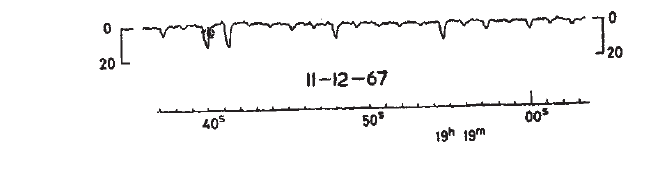
\includegraphics[width=0.8\textwidth]{pics/intro/pulses.png}
  \caption[A record of pulsating radio source]{A record of the pulsating radio
    source discovered in 1967 \citep{1969Natur.224..472H}}
  \label{fig:pulse}
\end{figure}
%

As more pulsars were discovered, slowing down of pulsar rotations were also discovered that enabled the estimation of spin-down luminosity from their angular velocity $\Omega$ and angular acceleration $\dot{\Omega}$ or the period $P$ and its derivative $\dot{P}$
%
\begin{equation}\label{eq:spin_down}
	  L_{d} = -I\Omega\dot{\Omega} = 4\pi^2 I\frac{\dot{P}}{P^3}
\end{equation}
%
where $I$ is the moment of inertia of the pulsar.
For the Crab pulsar with period $P=33$~ms and $\dot{P}=4.2\times 10^{-13}$ \citep{1968IAUC.2113....1L}, its spin-down luminosity is $10^{39}$~erg/s which agreed with the observed luminosity.

Our current knowledge attributes the spin-down of the pulsars to their magnetic field. For the simplest case, the pulsar magnetic can be modeled as a magnetic dipole with strength $\mu$.
As the giant magnetic dipole of pulsar is rotating, it is radiating away its rotational energy at the luminosity
%
\begin{equation}\label{eq:dipole_rad}
	L_{d} = \frac{2}{3}\frac{\mu^2\Omega^4}{c^3}.
\end{equation}
%
Equating Equation~\ref{eq:spin_down}  and Equation~\ref{eq:dipole_rad} can lead to an estimation of magnetic field at the surface of the neutron star
%
\begin{equation}
		B_0 = 3.2\times 10^{19}\sqrt{P \dot{P}}\,\mathrm{G}.
\end{equation}
%
For normal pulsars parameters, the resulting surface magnetic fields are of order $10^{12}$~G.
Such high magnetic fields also eliminate the possibility that radio pulsars being white dwarfs and establish rotating neutron stars as the standard theoretical explanation of pulsars.

Apart from radio emission, neutron stars are also visible in X-ray and $\gamma$-ray bands. Several neutron stars including the Crab \citep{1974Natur.251..397K} and Vela \citep{1975ApJ...200L..79T} were discovered to have pulsed $\gamma$-ray emissions at the period as the radio pulses. 
Geminga pulsar, on the other hand, was a radio-quiet $\gamma$-ray source with soft X-ray pulses \citep{1992Natur.357..222H} suggesting the $\gamma$-ray and radio emissions origin from different regions.
The {\it Fermi} satellite discovered over 130 $\gamma$-ray pulsars \citep{2010ApJS..188..405A}.
These $\gamma$-ray pulsars can be classified into three groups: millisecond pulsars, young radio-loud pulsars and young radio-quiet sources.
 Many neutron stars are also X-ray sources. Their X-ray radiation is usually made up of two components: a thermal component from the surface cooling and a non-thermal component from the magnetospheric emission \citep{2006csxs.book..279K}.
 
 \subsection{Structure of neutron stars}
 \label{sec:intro-structure}
 
The structure of a non-rotating unmagnetized neutron star is governed by Equation~\ref{eq:TOV} together with the equations of state.
The equation of state must be determined from the underlying physics that describes the interaction of the neutron-rich nuclear matter.
Depending on the density, the structure of a neutron star can be divided into two regions: the core and the crust. 
The core of a neutron star refers to the region where $\rho>\rho_{\rm nuc}$ with $\rho_{\rm nuc}=2.8\times 10^{14}$g/cm$^3$ being the density of nuclear saturation which accounts for $\sim 99\%$ of the total mass of the star.
The outer layer where $\rho<\rho_{\rm nuc}$ is the neutron star crust.
%
\begin{figure}[h]
  \centering
  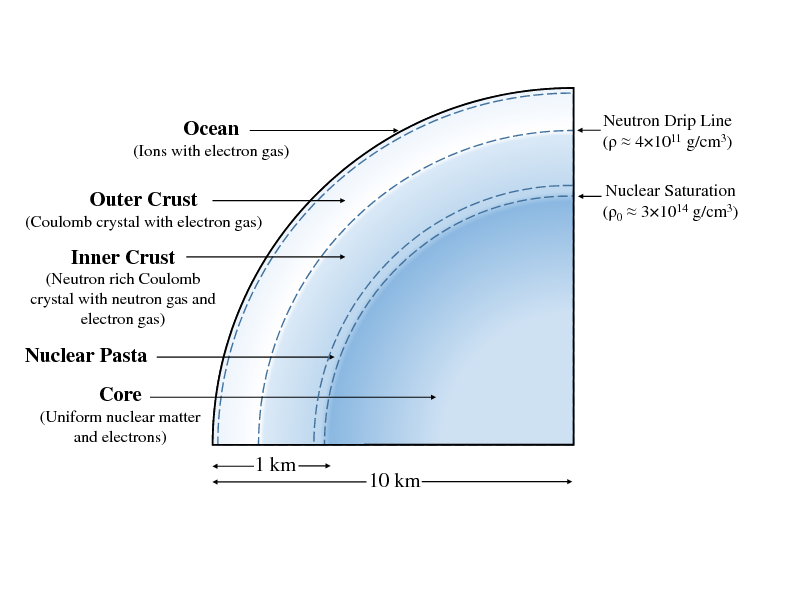
\includegraphics[width=0.8\textwidth]{pics/intro/NS_structure.png}
  \caption[A cartoon illustrates the structure of a neutron star] {A cartoon illustrates the structure of a neutron star \citep{2017RvMP...89d1002C}}
  \label{fig:NS-structure}
\end{figure}
%
\subsubsection{Core}
The neutron star core is composed of a mixture of neutrons, protons and electrons and possibly muons.
All constituents are highly degenerate and interact through nuclear force to form a strongly non-ideal liquid.
Calculation for the equation of state and the composition of highly degenerate nuclear matter from nuclear physics is very uncertain especially at high density $\rho>2\rho_{\rm nuc}$.
Exotic forms of matter like hyperionic matter ($\Sigma^-$ and $\Lambda$ hyperons), pion condensate, kaon condensate and quark matter might exist at such a high density.  
\citet{1959NucPh..13..655M} predicted that neutron in neutron stars can become superfluid.
The neutron gas can form superfluid through the singlet-state ($^1 S_0$) Cooper paring [see \citet{2003RvMP...75..607D} for a review].
The critical temperature $T_{\rm crit}$ below which the crustal neutrons become superfluid is sensitive to uncertainties in modeling many-body strong interactions. The characteristic value is $T_{\rm crit} \lesssim 10^{10}$~K [e.g. \citet{1999PhyU...42..737Y,2001LNP...578...30L}], with significant uncertainties \citep{2004ARA&A..42..169Y, 2009ApJ...707.1131P,2012MNRAS.422.2632H,2015PhRvC..91a5806H}.

%
\begin{figure}[h]
  \centering
  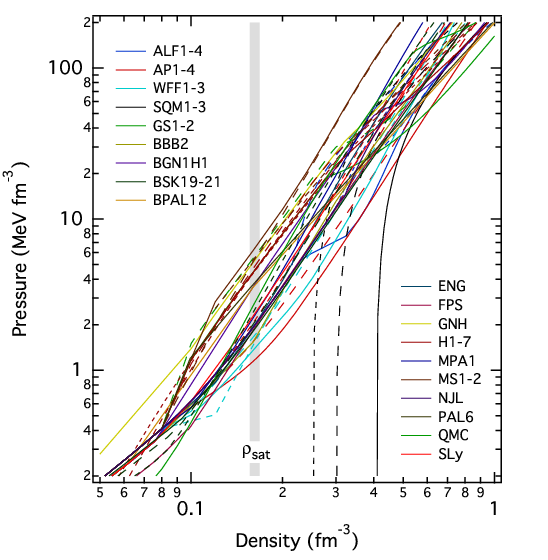
\includegraphics[height=0.4\textwidth]{pics/intro/eos.png}
  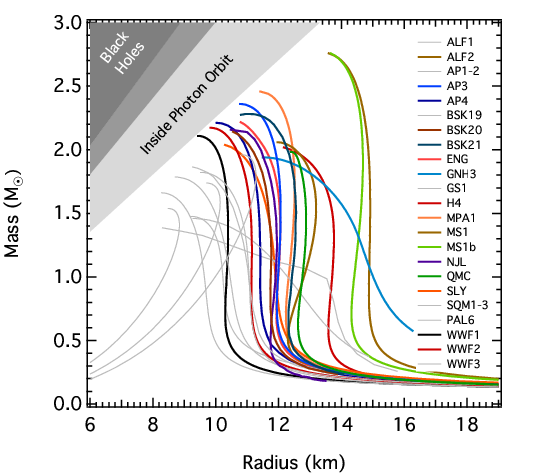
\includegraphics[height=0.4\textwidth]{pics/intro/mass-radius.png}
  \caption[Equation of state and mass-radius relation for neutron stars] {{\it Left:} Pressure as a function of density for various theoretical models. {\it Right:} Mass-radius relation for various neutron star equation of state \citep{2016ARA&A..54..401O}}
  \label{fig:NS-eos}
\end{figure}
%

The left panel of Figure~\ref{fig:NS-eos} shows different neutron star equations of state from various theoretical models and the right panel shows the resulting mass-radius relation from the corresponding equation of state.
Observational constraints of the neutron star equation of state mainly come from the measurements of mass and radius of neutron stars.
The determination of J1614-2230 to have mass $2M_\odot$ \citep{2010Natur.467.1081D} can eliminate all theoretical models with maximum mass smaller than it.

Neutrino emission is also generated through various channels in the neutron star and affects the cooling of neutron stars and the emissivity is very sensitive to the temperature $T$.
In the center of the core, Direct urca cooling (hereafter Durca) is the fastest neutrino emission mechanism
%
\begin{equation}
	   \dot{q}_\nu^D\sim 10^{27}\,T_9^6\, \mathcal{R}_D {\rm~erg~s}^{-1}{\rm cm}^{-3} \:\:\: (\rho\gtrsim 10^{15} {\rm~g~cm}^{-3}),
\end{equation}
%
where $\mathcal{R}_D\leq 1$ is a suppression factor that appears in the presence of 
superfluidity \citep{2001PhR...354....1Y}.  
However, it is activated only if the separation between the Fermi levels of protons and neutrons is sufficiently small, which occurs
at $\rho\gtrsim 10^{15}$~g~cm$^{-3}$.
Such high densities are only found in neutron stars with masses  $M \gtrsim 1.4 M_\odot$ \citep{1991PhRvL..66.2701L}.

Neutron stars with masses $M\lesssim 1.4M_\odot$ do not activate Durca, and the cooling occurs with a lower rate due to the modified urca reactions (hereafter Murca), which involve a spectator nucleon taking the excess momentum.
Murca occurs everywhere in the core with the cooling rate given by 
(\citealp{1979ApJ...232..541F}),
%
\begin{equation}
	\label{eq:Murca}
  \dot{q}_{\nu}^M\sim  7\times 10^{20}
  \,T_9^8 \left(\frac{\rho}{\rho_{\rm nuc}}\right)^{2/3} \mathcal{R}_M
    {\rm ~erg~s}^{-1}{\rm ~cm}^{-3},
\end{equation}
%
where $\rho_{\rm nuc}=2.8\times 10^{14}$~g~cm$^{-3}$ is the nuclear saturation density.
With the onset of proton or neutron superfluidity the Murca rate is suppressed by the 
factor $\mathcal{R}_M<1$, and the main cooling process becomes``Cooper pair cooling'' ---  
neutrino emission that accompanies the formation and breaking of Cooper 
pairs \citep{1976ApJ...205..541F,2009ApJ...707.1131P}. Its rate is given by
%
\begin{equation}
   \dot{q}_\nu^{CP}\sim 10^{21} \left(\frac{\rho}{\rho_{\rm nuc}}\right)^{1/3} T_9^7 
    \; f\left(\frac{T_{\rm core}}{T_{\rm crit}}\right) {\rm ~erg~s}^{-1}{\rm ~cm}^{-3}, 
\end{equation}
%
where the numerical factor $f(T_{\rm core}/T_{\rm crit})$ describes the temperature dependence of the Cooper pair cooling; $f=0$ at $T_{\rm core}>T_{\rm crit}$, $f$ steeply reaches a maximum at $T_{\rm core}\approx 0.8 T_{\rm crit}$ and steeply declines at $T_{\rm core}<0.5 T_{\rm crit}$.
%
\begin{figure}[h]
  \centering
  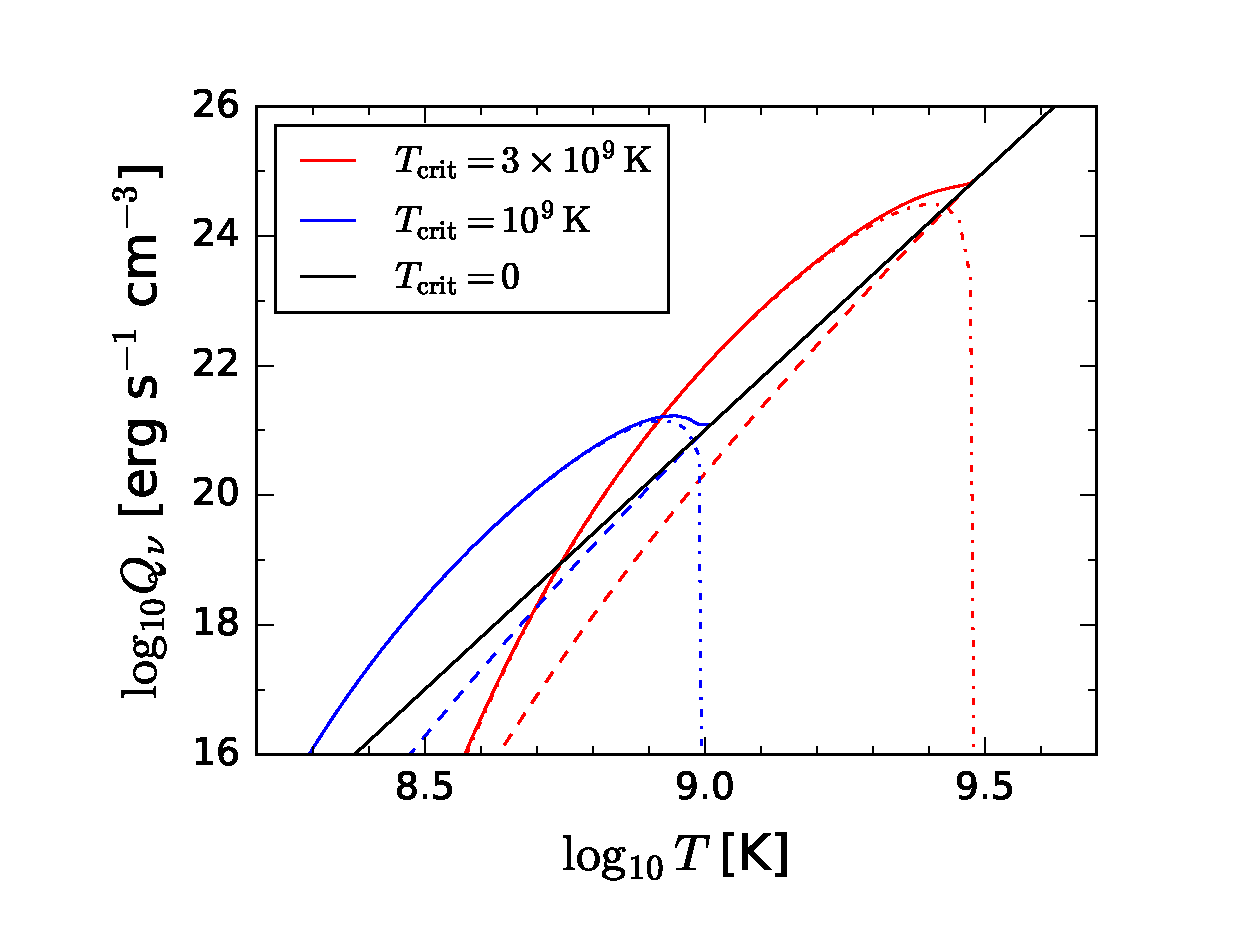
\includegraphics[height=0.6\textwidth]{pics/intro/qv.eps}
  \caption[Neutrino cooling rate in the core of neutron stars] {Neutrino cooling rate as a function of temperature in the core matter at density $\rho_{\rm nuc}=2.8\times 10^{14}$~g~cm$^{-3}$. Black curve shows Murca cooling assuming no superfluidity ($T_{\rm crit}<10^8$~K). Colored curves show the cooling of matter with non-superfluid protons and superfluid neutrons, for two cases: $T_{\rm crit}=10^9$~K (blue curves) and $T_{\rm crit}=3\times 10^9$~K (red curves). Dashed curve shows the Murca contribution and dash-dotted curve shows the Cooper pair contribution; the net cooling rate is shown by the solid curve.
The triplet-state neutron pairing is assumed (model B in \citealp{2001PhR...354....1Y})}
  \label{fig:NS-qv}
\end{figure}
%

\subsubsection{Crust}

The neutron star crust is elastic solid composed of Coulomb lattice of nuclei with degenerate electrons and neutrons.
The degenerate electrons are ultra-relativistic and the electron capture process $e^-+p\rightarrow n + \nu_e$ becomes more effective with increasing density which makes the matter more neutron-rich.
In the outer crust where density is lower than the neutron drip density $\rho_0=4\times 10^{11}$~g/cm$^3$, the pressure is dominated by the degenerate electron gas.
In the inner crust $\rho>\rho_0$,  neutrons start to drip out of the nuclei and form a free fermionic gas. Heavy nuclei, degenerate electrons, degenerate neutrons and free neutrons coexist and the pressure is dominated by the free neutrons.
Close to the core-crust interface, nuclei are more energetically favorable to have anisotropic shapes \citep{1983NuPhA.407..571R}. 
These new phases of nuclear matter are named as nuclear pasta phases. They are the transitive states to the uniform nuclear matter in the core and can have observational signature on the transport properties of neutron stars  \citep{2017RvMP...89d1002C}. 
The outermost $\sim 100$~m of the crust, called envelope or ocean, is low-density ($\rho<10^9$~g/cm$^3$) liquid.
Their chemical composition can be heavy nuclear like iron or light element if the neutron star accretes matter from its companion in a binary system.

Even though the crust only accounts for a small fraction of the mass of the neutron star, it is crucial for many astrophysical phenomena of the neutron stars.
The core of the neutron has high thermal conductivity and remain isothermal, and it is the thermal properties of the crust that govern the heat transport rate and therefore the surface temperature of the neutron star.
The specific heat of the crust are dominated by degenerate electrons and ions \citep{2015SSRv..191..239P}. Neutrons also contribute to the specific heat above the neutron drip point, however, their contributions will be greatly reduced once neutrons become superfluid.
The thermal conductivity is governed by the degenerate electron gas and increases with density. A static temperature profile in the crust will exhibit a constant temperature in most part of the crust with a sharp temperature gradient sustained in the envelope that governs the surface temperature of the neutron star.   
With the presence of strong magnetic fields, it is more energetically favorable for the degenerate electrons to stay in the lowest Landau level. 
Especially, when the energy of the lowest Landau level $\hbar e B/m_e c$ is larger than the rest mass energy $m_e c^2$ (i.e. $B>B_{\rm QED}\equiv m_e^2 c^3/\hbar e=4.4\times 10^{13}$~G), all electrons are confined in the lowest Landau level.
Therefore, thermal conductivity is enhanced in the direction parallel to the magnetic fields and reduced in the perpendicular direction \citep{1996A&A...306..999P,1996A&A...314..341P}.

Neutrino emissions in the crust become efficient cooling mechanism once internal or external heating increase the temperature above $10^9$~K. 
The main channels for neutrino emission in the crust are plasmon decay, electron-nucleus bremsstrahlung, electron-positron annihilation and electron synchrotron radiation if strong magnetic fields are present \citep{2001PhR...354....1Y}.

\section{Magnetars}
\label{sec:intro-magnetars}

% TODO: Introduce magnetars, and open up the historical observation discussions
Magnetars are a class of neutron stars with ultra-strong magnetic fields. 
They exhibit giant flares, bursts and outbursts in the band of hard X-ray to soft $\gamma$-rays. 
Unlike normal pulsars which are powered by the rotational energy, magnetar activities typically have radiation luminosity much larger than their spin-down power.
The ultimate energy source of their violent radiative activities is the strong magnetic field inside and outside the neutron stars.

\subsection{Discovery}
\label{sec:intro-magnetar-discovery}

In 1979, the interplanetary probes Venera 11 and 12 reported repeated bursts in the band of hard X-ray and soft $\gamma$-ray \citep{1979SvAL....5...87M}.
At first, these events were first classified as classical Gamma Ray Bursts (GRBs), but the repeated bursts in the star-forming Dorado region in the Large Magellanic Cloud including a giant flare \citep{1979Natur.282..587M} suggested they were a new class of high energy radiative events. 
The bursts exhibited strong evidence that they came from neutron stars.
They had very short rise time $\sim 15$~ms, implying the a relativistic motion over the distance of the size of a neutron star.
A $8$~s pulsating period was also observed in the tail of the light curve is consistent with the rotational period of a neutron star, though much slower than other young neutron stars like the $33$~ms Crab pulsar.
As more repeated bursts were subsequently discovered including SGR 1806-20 \citep{1987ApJ...322L..21K,1987ApJ...320L.111L} which showed around $100$ bursts between 1978 and 1986, these sources were finally recognized as a new class of high energy radiative events, Soft Gamma Ray Repeaters (SGRs).

Meanwhile, another mysterious class of objects, Anomalous X-ray Pulsars (AXPs) were also discovered whose strong X-ray luminosity exceeded the spin-down power.
The first object was discovered in the supernova remnant CTB 109 using the Einstein observatory \citep{1980Natur.287..805G}, with a spin period of $3.5$~s \citep{1981Natur.293..202F}.
Later, two other sources were discovered, 1E 1048.1-5937 \citep{1986ApJ...305..814S} and 4U 0142+61 \citep{1994MNRAS.267..490H,1994ApJ...433L..25I}. They all showed unusually soft X-ray spectra, making AXPs a new class of objects.

\citet{1995MNRAS.275..255T,1996ApJ...473..322T} suggested that SGRs are actually neutron stars with ultra-strong magnetic fields $10^{14}-10^{15}$~G, the magnetars.
In their model, repeated bursts are powered by the decay of magnetic energy from the ultra-strong magnetic field.
\alfven waves launched from the interior of the magnetar dissipate their energy in the magnetosphere creating an optically thick pair plasma fireball that gives rise to the soft-ray emission.
\citet{1996ApJ...473..322T} also suggested that AXPs are also magnetars and should exhibit repeated bursts.

In 1998, the first SGR spin-down rate was measured for SGR 1806-20 \citep{1998Natur.393..235K}, reporting a surface dipole magnetic field $8\times 10^{14}$~G. The same measurement for SGR 1900+14 were followed shortly \citep{1999ApJ...510L.115K} with magnetic field $2-8\times 10^{14}$~G.
The identification of SGRs as magnetars were confirmed by the two measurements.
SGR-like bursts were also discovered for AXPs later \citep{2002Natur.419..142G,2003ApJ...596L..71K}, and bursts are known to be a characteristic property of AXPs.
Eventually, the astrophysical community accepted magnetars as the standard explanation for SGRs and AXPs.

Up to now, there are 29 magnetars discovered, including 15 SGRs and 14 AXPs [cf. McGill Online Magnetar Catalog at http://www.physics.mcgill.ca/~pulsar/magnetar/main.html \citep{2014ApJS..212....6O}].
Figure~\ref{fig:ppdot} shows the relation between period $P$ and its time derivative $\dot{P}$ for various pulsars and magnetars.
Due to their high dipole magnetic fields, magnetars have higher spin-down rate and larger periods, and they all sit on the top-right corner of the figure.
%
\begin{figure}[h]
  \centering
  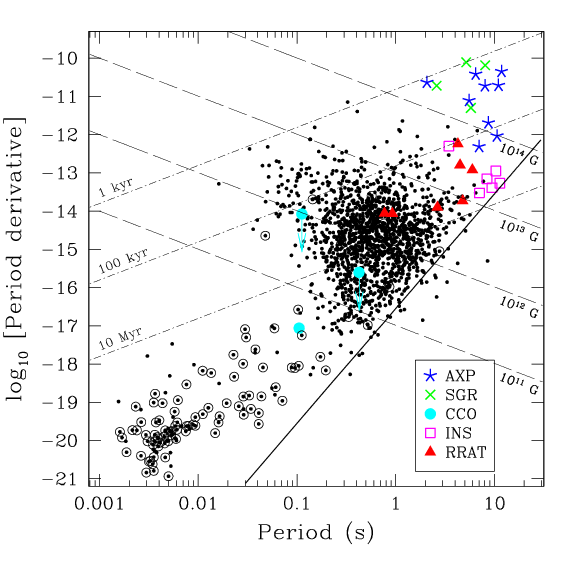
\includegraphics[width=0.6\textwidth]{pics/intro/ppdot.png}
  \caption[$P-\dot{P}$ diagram for pulsars and magnetars]{$P-\dot{P}$ diagram for pulsars and magnetars \citep{2010PNAS..107.7147K}.}
  \label{fig:ppdot}
\end{figure}
%
\subsection{Magnetar Activities}
\label{sec:magnetar-activities}

Magnetars exhibit both transient and persistent high energy radiations in forms of hard X-ray and soft $\gamma$-ray.
The transient events including soft $\gamma$-ray bursts, giant flares and outbursts.
The term burst refers to short millisecond events and giant flare refer to those violent bursts releasing energy higher than $10^44$~erg.
Outburst, on the other hand, refer to longer events with an exponential decaying afterglow on the timescale of months to years.

\subsubsection{Bursts}
Soft $\gamma$-ray bursts are the the most common transient events for magnetars. Both SGRs and AXPs exhibit bursts with a full spectrum of burst rate.
Some extremely active sources like SGR 0526-66 can become inactive for the subsequent decades \citep{2003ApJ...585..948K,2009MNRAS.399L..74T} while some quiet source like 1E 2259+586 can suddenly enter an active phase with hundreds of bursts  \citep{2003ApJ...588L..93K}.

The bursts have peak luminosity ranging $10^{36}$ to $10^{43}$~erg/s and sharp rise time from millisecond to second, with a log normal distribution peaking near $100$~ms.
The repeated bursts have power-law distribution, positive correlation between waiting times of successive events, log-normal waiting time distribution and no correlation between waiting times and intensities \citep{1996Natur.382..518C}.

\subsubsection{Giant Flares}
Giant flares are the most catastrophic radiative events of magnetars. 
There have been three events recorded up to now, all come from different sources: SGR 0526-66 on March 5, 1979 \citep{1980ApJ...237L...7E}, SGR 1900+14 on August 27, 1998 \citep{1999Natur.397...41H} and SGR 1806-20 on December 27, 2004 \citep{2005Natur.434.1098H,2005ApJ...624L.105M,2007ApJ...661..458B}.
The peak luminosity of giant flares range from $10^{44}$ to $10^{47}$~erg/s.
Figure~\ref{fig:gf-light-curve} shows the light curve for the 2004 giant flare SGR 1806-20. 
The light curve consists of two parts: an initial spike $\sim 0.2$~s followed by a long decaying tail lasting for $\sim 400$~s modulated by the rotational period of $7.56$~s.
Most energy (over $10^{46}$~erg) is released during the initial peak while the tail only radiates $10^{44}$~erg of energy.
%
\begin{figure}[h]
  \centering
  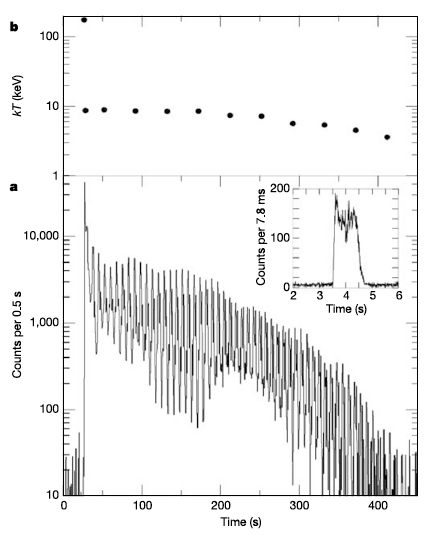
\includegraphics[width=0.5\textwidth]{pics/intro/gf.png}
  \caption[Light curve for the 2004 giant flare SGR 1806-20]{Light curve for the 2004 giant flare SGR 1806-20 \citep{2005Natur.434.1098H}.}
  \label{fig:gf-light-curve}
\end{figure}
%

\subsubsection{Outbursts}

Magnetar outbursts are characterized a sudden increase of X-ray luminosity up to $10^{36}$~erg/s, 10-1000 times of the quiescent level of radiations \citep{2004ApJ...609L..21I,2004ApJ...605..368G,2008A&ARv..15..225M,2011ASSP...21..247R}.
The outbursts are generally associated with radiative and timing anomalies such as spectral hardening, change in pulsed fraction and pulse profiles, multiple short X-ray bursts and glitches.
The light curves of outbursts usually show a long exponential decay following the bursts on the time scale of months to years. 
Figure~\ref{fig:outburst-light-curve} plots the light curves for eight different outbursts.
%
\begin{figure}[h]
  \centering
  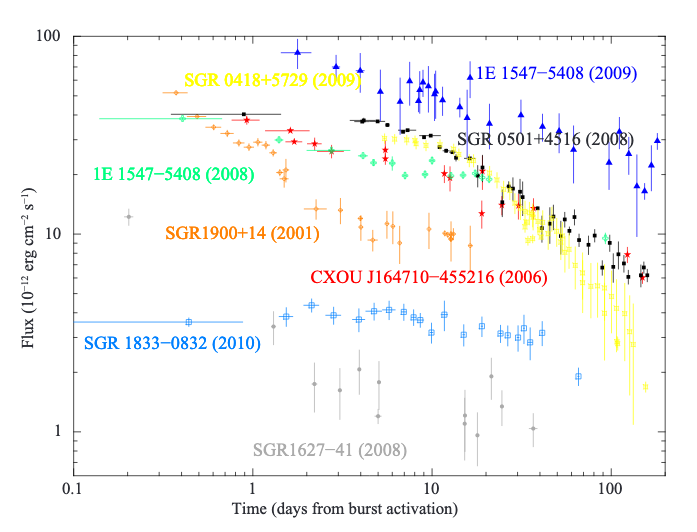
\includegraphics[width=0.6\textwidth]{pics/intro/outbursts.png}
  \caption[Light curves of eight magnetar outbursts]{Light curves of eight magnetar outbursts \citep{2011ASSP...21..247R}.}
  \label{fig:outburst-light-curve}
\end{figure}
%

Some magnetars have very low quiescent luminosities $<10^{33}$~erg/s and are discovered only when their X-ray luminosity increases by a factor of $100-1000$ during the outburst.
These magnetars are named as transient magnetars, and the first transient magnetar was discovered is XTE J1810-197 \citep{2004ApJ...609L..21I} whose flux decayed on the time scale of a year \citep{2007Ap&SS.308...79G}.

\subsubsection{Persistent emissions}

In the quiescent phase, magnetars can be divided into two different classes: the persistent magnetars and the transient magnetars.
The persistent magnetars like 1E 2259+586 or 4U 0142+61 have high quiescent luminosity $>10^{33}$~erg/s while the transient magnetars like XTE J1810-197 or SGR J1745-2900  have low quiescent luminosity.
The X-ray spectra of transient magnetars can be well modeled by a single blackbody component with temperature $k_B T\sim 0.15-0.3$~keV while persistent magnetars usually show a power-law component in addition to the blackbody component with $k_B T\sim 0.3-0.5$~keV \citep{2014ApJS..212....6O}.
The surface luminosity of persistent magnetars show a narrow range around $10^{35}$~erg/s \citep{2006ApJ...650.1070D} corresponding to the surface temperature of $0.3-0.5$~keV consistent with their X-ray spectra.
For a thousand-year-old neutron star usually have core temperature $T_{\rm core}\sim 10^8$~K and surface temperature $T_{\rm surf}\sim 10^6$~K \citep{2004ARA&A..42..169Y}, corresponding to the thermal luminosity of $10^{33}$~erg/s.
The surface temperatures of persistent magnetars are significantly higher than the surface temperature of normal neutron stars.
It is proposed that the high temperatures are sustained by the magnetic energy stored in the magnetars \citep{1992ApJ...392L...9D,1992AcA....42..145P} .

\subsection{Theoretical Models}
\subsubsection{Internal dynamics and crustal failures}
A young magnetar can have a strong toroidal magnetic component as a result of magnetohydrodynamical relaxation after its birth \citep{2009MNRAS.397..763B}.
Since the interior of a neutron star is a perfect, magnetic fields are frozen into the electron fluid and magnetic fields can move mainly through the drift of electrons with respect to the neutrons and ions.
Therefore the evolution of magnetic fields is slow in the magnetar, and main through the two process: ambipolar diffusion and Hall drift \citep{1992ApJ...395..250G}.

Ambipolar diffusion results from the motion of electron-proton plasma through the neutron fluid. 
Due to the difference of proton and electron mass, protons feel the frictional force from the collision with neutrons while electrons almost move freely.
In the core, the ambipolar diffusion  develops on the timescale $t_{\rm amb}\sim 10^3 (T_9/k_{-5}B_{16})^2$ \citep{2016ApJ...833..261B} where $T$ is the core temperature and the wave number $k\sim 10^{-5}$~cm$^{-1}$ characterizes the length scale of magnetic field variation $\pi/k$.
Pressure gradient is generated by the ambipolar diffusion but will be erased by weak interactions $e+p\rightarrow n$ \citep{1992ApJ...395..250G,2016ApJ...833..261B}.
The ambipolar diffusion tends to dissipate magnetic energy and heat up the magnetar, and the process stalls as the core temperature stalls.

Hall drift is a result of electron motion relative to ions with the velocity $\boldsymbol{v}_H = -\boldsymbol{j}/en_e$ where $\boldsymbol{j}$ is the current and $n_e\sim 10^{37}$~cm$^{-3}$ is the electron number density.
Even though Hall drift conserves energy, it can cascade energy to smaller scales and dissipate the energy through the Ohmic dissipation \citep{1992ApJ...395..250G}.
Numerical simulations of Hall evolutions in the neutron star in 2D and 3D have been studied by \citep{2009A&A...496..207P, 2016PNAS..113.3944G,2018MNRAS.473.2771B}.

Magnetar crust, like the neutron star crust, is made up of nuclear Coulomb lattices.
The magnetar crust is incompressible and immune to cracks and slips due to the huge hydrostatic pressure \citep{2003ApJ...595..342J} and magnetic fields \citep{2012MNRAS.427.1574L}.
However, the Coulomb lattice can yield to shear stresses and give rise to plastic failures.
Molecular dynamics simulations by \citet{2009PhRvL.102s1102H} and \citet{2010MNRAS.407L..54C} that plastic failures are triggered when the elastic strain exceeds the critical value $s_{\rm cr}\approx 0.1$ as shown in Figure~\ref{fig:plastic-md}.
Shear magnetic stress can be generated and accumulated in the crust through the ambipolar diffusion and the Hall drift \citep{1996ApJ...473..322T,2011ApJ...727L..51P}, and trigger the failures when it reaches $s_{\rm cr}\mu$ where $\mu$ is the shear modulus of the crustal material.
The crustal failures will give rise to surface motions of magnetic fields which can release magnetic energy into the magnetosphere.
%
\begin{figure}[h]
  \centering
  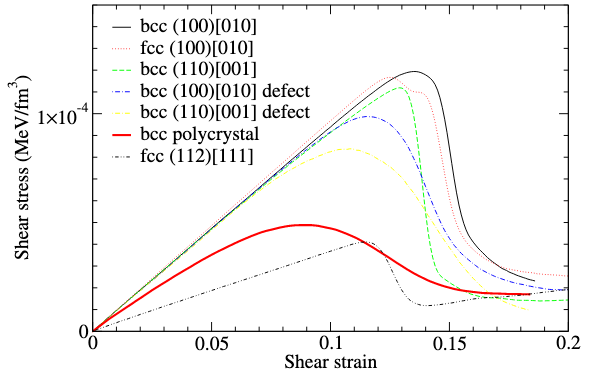
\includegraphics[width=0.6\textwidth]{pics/intro/plastic.png}
  \caption[Relation between shear stress and strain of materials in the neutron star crust]{Relation between shear stress and strain of materials in the neutron star crust for different crystal structure from the molecular dynamics simulations by \citet{2009PhRvL.102s1102H}.
  Plastic failures are triggered and release the shear stress when strain is above $\gtrsim 0.1$.}
  \label{fig:plastic-md}
\end{figure}
%

When the plastic flow is triggered, plasma viscosity will reduce the magnetic stress as well as dissipate magnetic to heat.
In response, the heated crustal material will be softened with $s_{\rm cr}$ reduced \citep{2010MNRAS.407L..54C}.
The interplay between the thermal and mechanical effects leads to the idea of thermoplastic instabilities \citep{2014ApJ...794L..24B}.
Thermoplastic waves are launched when heat released from a seed failure site diffuses to the neighboring materials and soften its critical stress below the existing shear magnetic stress.
A front of plastic failures therefore propagate in the crust, resembling the deflagration front.
The wave front propagates at the $v\sim (\chi B^2/4\pi\eta)^{1/2}$, where $\chi \sim 10$cm$^2$/s is the heat diffusion coefficient and $\eta$ is the viscosity.
Figure~\ref{fig:tpw} show the structure of the thermoplastic wave front, with $b$ being the scale magnetic, $U_{\rm th}$ being the thermal energy and $\mu_B=B^2/4\pi$.
%
\begin{figure}[h]
  \centering
  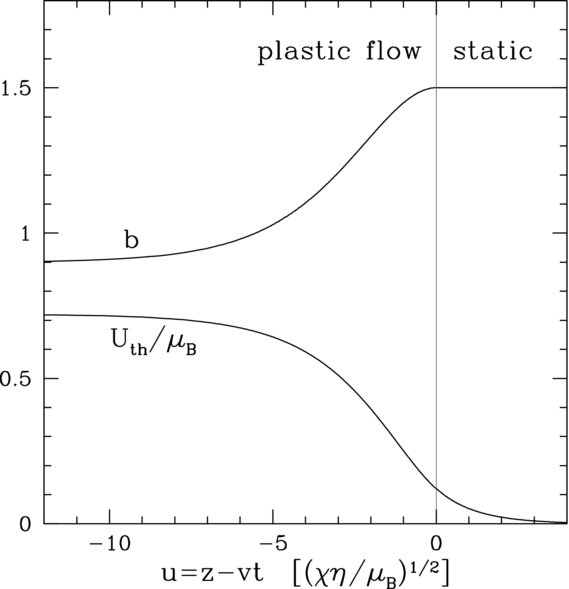
\includegraphics[width=0.6\textwidth]{pics/intro/tpw.jpg}
  \caption[Structure of the thermoplastic wave front]{structure of the thermoplastic wave front \citep{2014ApJ...794L..24B}.
  $b$ being the scale magnetic, $U_{\rm th}$ being the thermal energy and $\mu_B=B^2/4\pi$.}
  \label{fig:tpw}
\end{figure}
%

\subsubsection{Transient events}
The hard X-ray produced during giant flares and bursts must be produced outside the magnetars. 
Therefore magnetic energy must be ejected from the interior of the star to power the emission.
In the original proposal by \citet{1995MNRAS.275..255T,1996ApJ...473..322T}, magnetic energy is ejected from the interior into the magnetosphere in the form of \alfven waves.
The triggering mechanism could be the MHD instability in the liquid core or a sudden failure of the solid crust at the core-crust interface due to the build up of magnetic stress \citep{1995MNRAS.275..255T,2001ApJ...561..980T}.
Excitation of core motions with displacement $\xi$ will release energy up to $\sim E_{\rm mag}(\xi/R)^2$ where $E_{\rm mag}\sim 10^{48}$~erg is the magnetic energy in the core and $R$ is the radius of the magnetar.
The magnetic energy carried by \alfven waves are fast dissipated through turbulent cascade or magnetic reconnection.
An alternative mechanism that can trigger the release of magnetic energy into the magnetosphere is through a gradual deformation of the magnetosphere followed by a sudden of the free magnetic energy built up in the magnetosphere \citep{2003MNRAS.346..540L,2010MNRAS.407.1926G, 2013ApJ...774...92P}.
The twist of magnetosphere can be a result of crustal motions, especially plastic failures that occurs in the crust.
Strongly deformed magnetospheres can undergo global instabilities \citep{2002ApJ...572..432U}.
Numerical simulations by \citep{2013ApJ...774...92P} have demonstrated that the magnetosphere becomes unstable once the twist angle exceeds a critical value.
The free magnetic energy is released suddenly to power a flare.
This process also involves the formation of a current at the equator of the magnetosphere as shown in Figure~\ref{fig:overtwisted-magnetar}.
The current is tearing unstable and magnetic reconnection takes place which fast dissipates the magnetic energy and ejects plasmoids.
%
\begin{figure}[h]
  \centering
  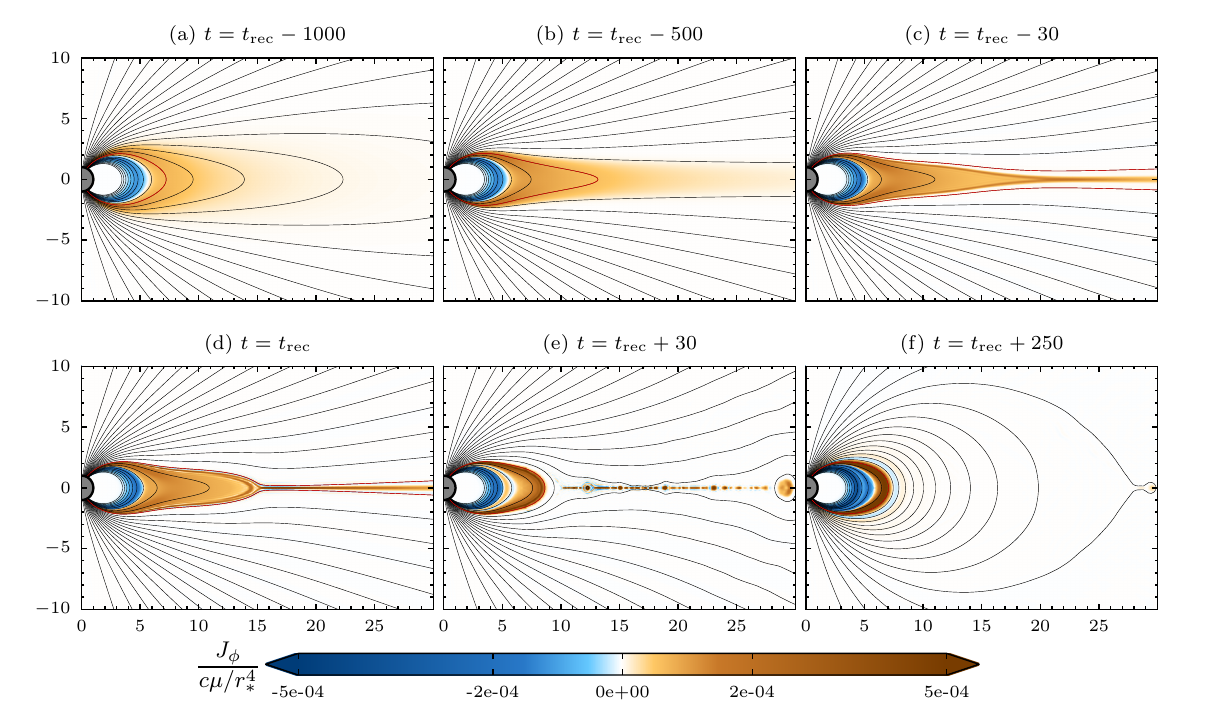
\includegraphics[width=\textwidth]{pics/intro/ffe-giant-flare.png}
  \caption[Formation of the equatorial current sheet in an over-twisted magnetar
    magnetosphere.]{Formation of the equatorial current sheet in over twisted magnetar
    magnetosphere. Color shows toroidal current density. Time is indicated in
    units of light crossing time of the star. \citep{2013ApJ...774...92P}}
  \label{fig:overtwisted-magnetar}
\end{figure}
%
The energy released during the initial spikes of giant flares are immediately thermalized, creating a fireball consisting of optically thick $e^\pm$ pair plasmas.
The evaporation of such pair plasma fireball produces the pulsating tail of the flare  \citep{1995MNRAS.275..255T,1996ApJ...473..322T}.
Besides, \alfven waves are also generated during the reconnection process.
Theses waves are trapped on the closed fields and dissipate either through nonlinear interactions \citep{1998PhRvD..57.3219T} or inside the magnetar \citep{2015ApJ...815...25L}.

\citet{2002ApJ...580L..69L} modeled the afterglow of the 1998 giant flare SGR 1900+14 by a sudden heating event in the crust.
In order to fit the observations, enormous amount of heat per unit mass is required in the outermost layer of the crust. 
How magnetic energy can heat the crust the crust to such a high level is still unclear. However, this phenomenological model has been applied to several transient magnetars to reproduce the observed light curve \citep{2013ApJ...770...65R,2014ApJ...786...62S}.

Less energetic magnetar outbursts are also considered to be trigger by the crustal motions.
Following the original ideas of \citet{1996ApJ...473..322T}, \citet{2011ApJ...727L..51P} argued that the outbursts are powered by localized releases of elastic energy in the crust  due to mechanical failures in the crystal lattice (the ``starquakes"). 
They modeled the build up of the elastic energy before each release as a result of the changing magnetic stresses, and have produced a phenomenological numerical model for the frequency of the outbursts and the magnitude of their energy release.  \citet{2012ApJ...750L...6P} have modeled the outbursts by computing the thermal flux emerging from the neutron star surface from an impulsive energy release in the crust. 


\subsubsection{Gradual untwisting of the magnetosphere}

Apart from releasing magnetic energy within a very short period of time, a twisted magnetosphere can also produce more persistent X-ray emissions through a gradual untwisting process \citep{2002ApJ...574..332T, 2009ApJ...703.1044B}.
\citet{2009ApJ...703.1044B} studied the dynamics of the twisted magnetosphere.
The nonzero $\nabla\times \boldsymbol{B}$ implies the existence of current in the magnetosphere, and the Ohmic dissipation will slowly untwist the magnetosphere.
Parallel electrical fields exist along the direction of $\boldsymbol{B}$ and lead to a longitudinal discharge voltage $\Phi_{\parallel}\sim 10^{10}$~V.
When $\Phi_{\parallel}$ is larger than a threshold value, creation of electron-positron pairs will occur and screen the parallel electrical field and therefore regulate the discharge voltage \citep{2007ApJ...657..967B}.
The main channel for pair production is through the resonant scattering of background photons.
Soft X-ray photons of a few keV from the thermal radiation of magnetars will be boosted by the electron Lorentz factor of $\gamma$ in the rest frame of electrons.
Electrons can then absorb and re-emit the photon if resonant conditions are satisfied, and the re-emitted photons have an energy boost $\sim \gamma^2$ which will produce more pairs in the magnetic field.
This process was demonstrated by the Particle-In-Cell (PIC) simulation by \citet{2017ApJ...844..133C}.

The untwisting of the magnetosphere proceeds in the following manner.
In the inner magnetosphere, a cavity with $\boldsymbol{j}=0$ is first developed which then expands and remove the current in the ``j-buldle'', the current carried by the twisted magnetosphere.
The footpoints of the j-bundle is considered to be hotter than the rest part of the magnetar surface since relativistic particles produced by the electron-positron discharge can bombard the footpoints.
As the j-bundle shrinks, the hotspot area $A$ should also shrink as well as the luminosity $L$ which gives rise to observational signatures.
Theoretical relation between $A$ and $L$ is given by$L\sim 1.33\times 10^{13} K A_{11}^2$~erg/s where $K = B_{14}\Phi_{\parallel 9}\psi$ where $\psi$ is the twisting angle.
Figure~\ref{fig:hot-spot} shows the evolution of hotspots observed for seven transient magnetars following their outbursts.
All the data points agree reasonably well with the theoretical $A-L$ relation.
%
\begin{figure}[h]
  \centering
  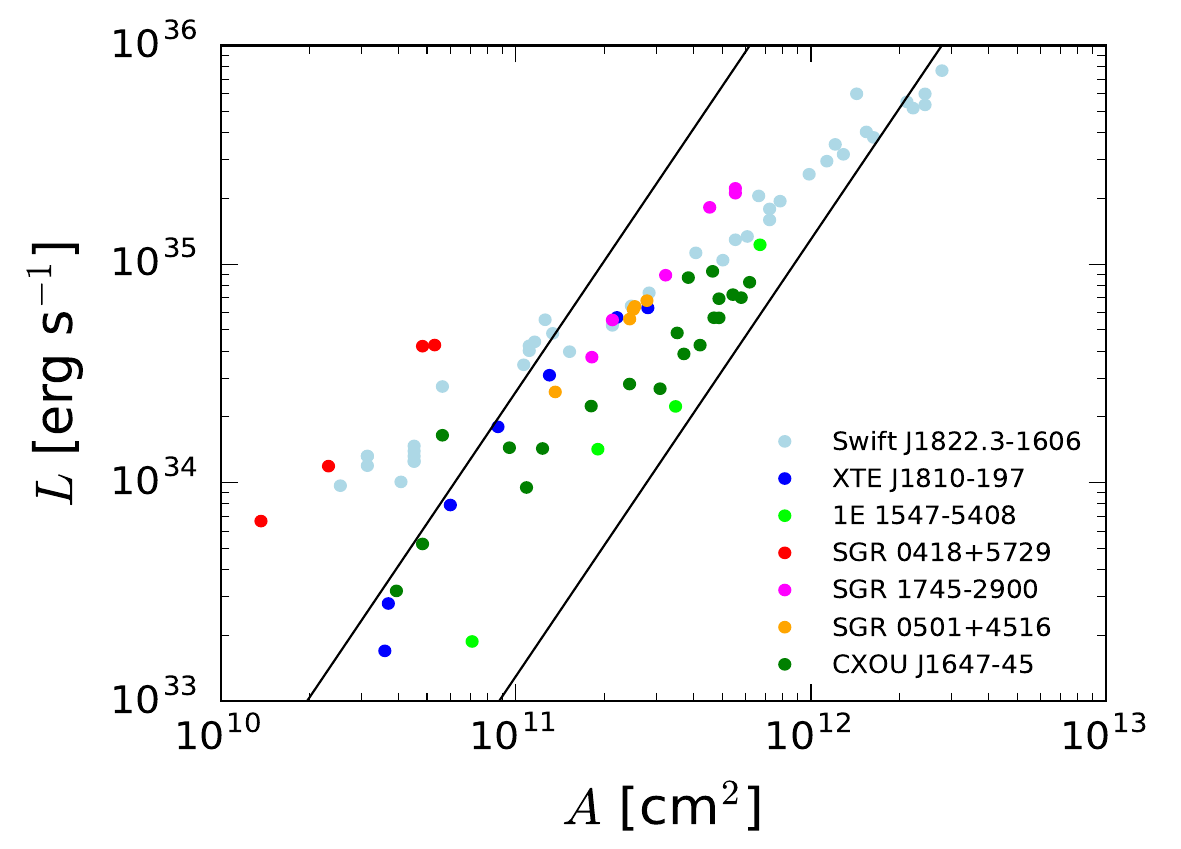
\includegraphics[width=0.6\textwidth]{pics/intro/hot-spot.png}
  \caption[The evolution of hotspots observed on transient magnetars following their outbursts]{The evolution of hotspots observed on transient magnetars following their outbursts. 
The theoretical prediction is shown by the strip between the two lines, 
$L \sim 1.3 \times 10^{33} K\,A_{11}^2$~erg~s$^{-1}$, where $K=B_{14} \Phi_9 \psi$.
The strip shown in the figure corresponds to $1<K<20$. Data for SGR 1745-2900 are 
from \citet{2015MNRAS.449.2685C};
CXOU J1647-45 from \citet{2011ApJ...726...37W} and \citet{2013ApJ...763...82A};
Swift J1822.3-1606 from \citet{2012ApJ...754...27R};
SGR 0418+5729 from \citet{2010MNRAS.405.1787E};
SGR 0501+4516 from \citet{2009MNRAS.396.2419R};
XTE J1810-197 from \citet{2007Ap&SS.308...79G};
1E 1547-5408 from \citet{2008ApJ...676.1178H} and \citet{2010PASJ...62..475E}.
The distance to 1E~1547-5408 was changed to 4~kpc following  
\citet{2010ApJ...710..227T} and \citet{2007ApJ...667.1111G}.
}
  \label{fig:hot-spot}
\end{figure}
%

Hard X-ray emissions are also produced through the resonant scattering process \citep{2013ApJ...762...13B}.
This process is sketched in Figure~\ref{fig:magnetar-loop}.
In the high magnetic field region $B>10^{13}$~G, upscattered photons are converted electron-pairs with $\gamma\approx 100(B/B_{\rm QED}$ where $B_{\rm QED}=4.4\times 10^{13}$~G.
The electron-positrons pairs form an outflow which is influenced by the radiative loss through the resonant scattering.
When the outflow of pairs reaches the region with low magnetic fields $B<10^{13}$~G, they have $\gamma\sim 1$, and upscattered photons are then able to escape leading to the hard X-ray radiation observed.
This picture provides good fit for the phase-resolved hard X-ray spectra of several magnetars \citep{2014ApJ...786L...1H,2014ApJ...789...75V,2015ApJ...807...93A}.
%
\begin{figure}[h]
  \centering
  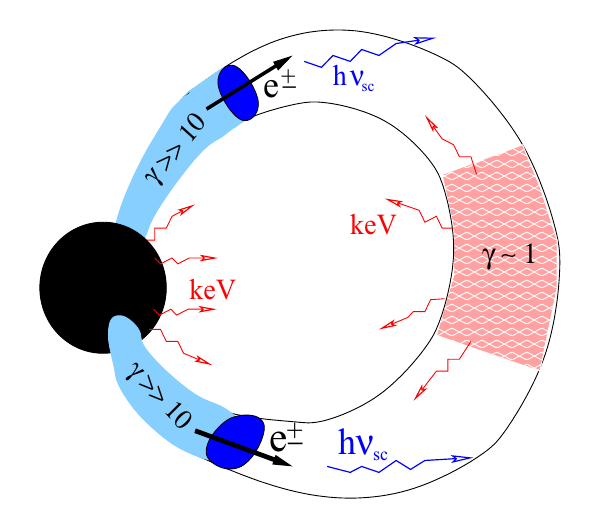
\includegraphics[width=0.5\textwidth]{pics/intro/magnetar-loop.png}
  \caption[Sketch of a twist magnetic loop.]{Sketch of a twist magnetic loop.
    Particles are accelerated in the blue region and resonantly scatter photons
    reflected from the pink region. The upscattered photons convert to pairs
    near the star, but can escape in the white region to form the observed X-ray
    spectrum \citep{2013ApJ...762...13B}.}
  \label{fig:magnetar-loop}
\end{figure}
%

\subsubsection{Magnetar heating}

The surface luminosity $10^{35}$~erg/s corresponds to the surface temperature of $T_s\approx 4\times 10^6$~K for a magnetar of radius $10-13$~km.
Typical neutron stars relax to a steady state temperature profile with constant heat flux on the conduction time $1-10$~yr after their birth.
The steady state temperature profile is isothermal at $T_{\rm core}$ in the core and most part of the crust with the temperature dropping smoothly to $T_s$ only in the outermost ``blanket'' layer $\rho<10^9$~K.
The relation of $T_{\rm core}$ and $T_s$ was established \citep{2003ApJ...594..404P} depending on the magnetic field strength and chemical composition in the blanket.
A core temperature $T_{\rm core}\gtrsim 10^9$~K is inferred from the surface luminosity of $10^{35}$~erg/s.
It is not clear how the core can sustain such a high temperature for $1-10$~kyr since neutrino emmision due to Murca process is effective in cooling the neutron star.
Heating of the core through the ambipolar diffusion may sustain the surface luminosity of $10^{35}$~erg/s. However, it requires extremely strong magnetic fields $B>10^{16}$~G and can only last for less than $1$~kyr \citep{2016ApJ...833..261B}.

Crustal heating has also been studied to explain the high surface temperature \citep{2014MNRAS.442.3484K}.
However, mechanical and ohmic heating in the crust are both limited.
Mechanical heating can only take place in the solid phase of the crust and its rate is constrained below $\sim\mu\dot{s}$ where $\mu$ is the shear modulus and $\dot{s}$ is the strain rate of deformation.
The maximum value of mechanical heating rate still falls short of the observed thermal luminosity.
The Ohmic heating rate reads $j^2/\sigma_{\rm el}$ where the conductivity $\sigma_{\rm el}\sim 10^{22}$~s$^{-1}$ for the relevant range of temperature and density in the crust \citep{2015SSRv..191..239P} and the current can be estimated through $j\sim \nabla\times B\sim \delta B/l$ as the variation of magnetic field $\delta B$ over the length scale $l$.
In order to match the observations, strong magnetic fields $\delta B>10^{16}$~G is required to vary on $l\sim 10^{4}$~cm which is not physical in the magnetar crust \citep{2016ApJ...833..261B}.

\section{This Dissertation}
\label{sec:intro-outline}

In this dissertation we will attempt to study some problems involving the dynamics of magnetic fields from the interior to the exterior of magnetars trying to answer the problem of how magnetar activities can be triggered in the crust and how magnetic energy can be dissipated to power radiations.

Chapter \ref{chap:mhd} will be a brief review of magnetohydrodynamics, its approximation in the magnetic dominated plasma -- Force-Free Electrodynamics as well as non-ideal corrections to magnetohydrodynamics.

Chapter \ref{chap:hall} will be devoted to the Hall evolution in the magnetar crust coupled with the mechanical response of the crustal material. We will propose a model for magnetar outbursts as a result of plastic crustal failures triggered by thermoplastic waves and Hall-mediated avalanches in the crust.

Chapter \ref{chap:plastic-damping} will study the interplay of magnetic evolution and crustal failures in a different setting. We will explore the fate of \alfven waves penetrating into the magnetar crust. The \alfven waves can dissipate their magnetic through triggering plastic failures which heat up the crust and power the afterglow.

Chapter \ref{chap:magnetosphere-dissipation} will focus on a competing process of \alfven wave dissipation in the magnetosphere, the turbulent cascade through the nonlinear interaction between waves. Compared with the dissipation inside the magnetar crust, turbulent dissipation is found to be slow unless the wave amplitude is much larger than the background magnetic field.

The work presented in this dissertation can be found in the following publications:
\begin{itemize}
	
\item \textit{Magnetar Outbursts from Avalanches of Hall Waves and Crustal Failures} 

Xinyu Li,  Yuri Levin and Andrei M. Beloborodov, The Astrophysical Journal, 189, 12, (2016), arXiv: 1606.04895

\item \textit{Plastic Damping of \alfven Waves in Magnetar Flares and Delayed Afterglow Emission}
 
Xinyu Li and Andrei Beloborodov, The Astrophysical Journal, 815, 25, (2015), arXiv: 1505.03465

\item \textit{Dissipation of \alfven Waves in Relativistic Magnetospheres of Magnetars}
 
Xinyu Li, Jonathan Zrake and Andrei Beloborodov, submitted to The Astrophysical Journal, arXiv: 1810.10493

\item \textit{Magnetar Heating}

Andrei Beloborodov and Xinyu Li, The Astrophysical Journal, 261, 20, (2016), arXiv: 1605.09077

\end{itemize}





% Local Variables:
% TeX-master: "../thesis"
% zotero-collection: #("16" 0 2 (name "Thesis"))
% End:

\zotelo{../thesis.bib}

\chapter{Magnetohydrodynamics (MHD)}
\label{chap:mhd}

\section{Ideal MHD}
\label{sec:ideal}

\subsection{Nonrelativistic ideal MHD}
Just like the dynamics of a system of particles on the scale much larger than their mean free path can be well described by hydrodynamics, magnetohydrodynamics (MHD) provides a description of the dynamics of current-carrying particle systems in the electromagnetic fields where the characteristic length scale of interest is much larger than the mean free path as well as the gyroradius of the charged particles.
In addition to the continuity equation
\begin{eqnarray}\label{eq:mhd-continuity}
	\frac{\partial \rho}{\partial t} + \nabla \cdot (\rho \boldsymbol{v})=0,
\end{eqnarray}
the momentum equation of the fluid in MHD is modified with the Lorentz force $\boldsymbol{j}\times \boldsymbol{B}/c$
\begin{eqnarray}\label{eq:mhd-vel}
	\rho \left(\frac{\partial \boldsymbol{v}}{\partial t} + \boldsymbol{v}\cdot \nabla \boldsymbol{v}\right) = -\nabla P +\frac{ \boldsymbol{j}\times \boldsymbol{B}}{c}.
\end{eqnarray}
The current $\boldsymbol{j}$ can be determined from the electrical field $\boldsymbol{E'}$ in the rest frame of the fluid through Ohm's law
\begin{eqnarray}\label{eq:ohm-fluid}
	\boldsymbol{j} = \sigma_{\rm el} \boldsymbol{E'}
\end{eqnarray}
where $\sigma_{\rm el}$ is the electrical conductivity.
For nonrelativistic fluid $v\ll c$, the Lorentz transformation of the electromagnetic field is $\boldsymbol{E'} \approx \boldsymbol{E} + \boldsymbol{v}\times \boldsymbol{B}/c$, and Equation~\ref{eq:ohm-fluid} can be written as 
\begin{eqnarray}\label{eq:mhd-j}
	\frac{\boldsymbol{j}}{\sigma_{\rm el}} = \boldsymbol{E} +\frac{ \boldsymbol{v}}{c}\times \boldsymbol{B}.
\end{eqnarray}
The ideal MHD limit applies when the fluid has perfect conductivity $\sigma_{\rm el}\rightarrow\infty$, and therefore 
\begin{eqnarray}\label{eq:mhd-vanshing-e}
	\boldsymbol{E}=-\frac{\boldsymbol{v}}{c}\times\boldsymbol{B}.
\end{eqnarray}
Magnetic fields are evolved according to Faraday's law
\begin{eqnarray}\label{eq:mhd-induction}
	\frac{\partial \boldsymbol{B}}{\partial t} = -c\nabla\times\boldsymbol{E} = \nabla\times(\boldsymbol{v}\times\boldsymbol{B}).
\end{eqnarray}
And the electrical field produced by the displacement current  is suppressed by a factor of $(v/c)^2$ for nonrelativistic fluid and therefore can be neglected.
Hence, Ampere's law implies
\begin{eqnarray}
	\boldsymbol{j}=\frac{c}{4\pi}\nabla\times \boldsymbol{B}.
\end{eqnarray}
The momentum equation (Equation~\ref{eq:mhd-vel}) now becomes
\begin{eqnarray}\label{eq:mhd-momentum}
	\rho \left(\frac{\partial \boldsymbol{v}}{\partial t} + \boldsymbol{v}\cdot \nabla \boldsymbol{v}\right) = -\nabla P + \frac{(\nabla\times \boldsymbol{B})\times\boldsymbol{B}}{4\pi} = -\nabla\left( P + \frac{B^2}{4\pi} \right) + \frac{\boldsymbol{B}\cdot\nabla\boldsymbol{B}}{4\pi}.
\end{eqnarray}
Equation~\ref{eq:mhd-continuity}, \ref{eq:mhd-momentum}, \ref{eq:mhd-induction} together with the equation of state for the fluid $P(\rho)$ and the divergence constraint of magnetic fields $\nabla\cdot\boldsymbol{B}=0$ form the full set of ideal nonrelativistic MHD equations.

\subsection{Waves in nonrelativistic ideal MHD}
Linearization of MHD equations for small perturbations using $\delta P = c_s^2\delta \rho$ where $c_s$ is the sound speed of the fluid leads to three modes of waves supported by MHD.
The first one is a purely shear transverse wave with perturbed magnetic field perpendicular to the background field.
This mode is called the \alfven wave with the dispersion relation 
\begin{eqnarray}
	\omega^2 = v_A^2 k_{\parallel}^2
\end{eqnarray}
where $k_{\parallel}$ is the wavevector component parallel to the background magnetic field.
$v_A\equiv B/\sqrt{4\pi\rho}$ is called the \alfven speed.
\alfven waves have group velocity along the background field and can therefore only transport energy in that direction.
The other two wave modes have dispersion relations
\begin{eqnarray}\label{eq:magnetosonic}
	\omega^2 = \frac{k^2}{2}\left[ c_s^2 + v_A^2 \pm\sqrt{(c_s^2-v_A^2)^2+4 c_s^2 v_A^2k_\perp^2/k^2}  \right]
\end{eqnarray}
where $k_\perp$ is the wavevector component perpendicular to the background magnetic field.
These two waves are called fast (with $+$ in Equation~\ref{eq:magnetosonic}) and slow (with $-$ in Equation~\ref{eq:magnetosonic}) magnetosonic waves. Compression of the fluid is involved in exciting these waves.

In MHD, nonlinear interactions between waves govern the chaotic behavior of turbulence.
This type of turbulence is called wave turbulence which is different from hydrodynamical turbulence in which interaction between vortices dominates.
The basic formulation of wave turbulence is reviewed in Appendix \ref{app:wave-turbulence} and more details can be found in \citet{2011LNP...825.....N}.

\subsection{Relativistic MHD (RMHD)}
For relativistic fluids, the ideal MHD equations can be more easily written down using the covariant equations of conservative quantities.
\begin{eqnarray}\label{eq:rmhd-covariant}
	\nabla_\mu (\rho u^\mu) &=& 0, \\
	\nabla_\mu T^{\mu\nu} &=& 0,\\
	\nabla_\mu F^{*\mu\nu}&=& 0.
\end{eqnarray}
Here $u^\mu$ is the 4-velocity field of the fluid, $F^{*\mu\nu}$ is the dual of the electromagnetic tensor $F^{\mu\nu}$ and $T^{\mu\nu}$ is the stress-energy tensor
\begin{eqnarray}
	T^{\mu\nu} = \left(\rho h + \frac{b^2}{4\pi}\right)u^\mu u^\nu + \left(P^2 + \frac{b^2}{8\pi}\right) g^{\mu\nu} - \frac{b^\mu b^\nu}{4\pi}
\end{eqnarray}
where $h= 1+\epsilon +P/\rho$ is the specific enthalpy with specific internal energy $\epsilon$, $b^\mu=u_\mu F^{*\mu\nu}$ is the magnetic field in the fluid frame and $g^{\mu\nu}$ is the metric tensor.
The ideal MHD condition of vanishing electrical in the fluid frame (Equation~\ref{eq:mhd-vanshing-e}) translates to $u_\mu F^{\mu\nu}=0$, which implies $E<B$ in the lab frame for both nonrelativistic and relativistic MHD.

\section{Force-Free Electrodynamics (FFE)}
\label{sec:ffe}

In a magnetic dominated relativistic plasma, where the magnetic energy density is much larger than the rest mass energy density $B^2/4\pi\gg \rho c^2$, a simple approximation of relativistic MHD can be applied where the plasma inertia is neglected.
This approximation is called Force-Free Electrodynamics (FFE).
In this section, we utilize units in which speeds are measured in units of the speed of light $c$, and electric ($\boldsymbol{E}$) and magnetic ($\boldsymbol{B}$) field values are normalized by $\sqrt{4 \pi}$. 

The dynamical equations are given by Maxwell's equations,
%
\begin{eqnarray}\label{eq:Maxwell}
	\frac{\partial\boldsymbol{B}}{\partial t}+\nabla\times \boldsymbol{E} = 0,
    \qquad
	\frac{\partial\boldsymbol{E}}{\partial t}-\nabla\times \boldsymbol{B} &=& -\boldsymbol{J} \, ,
\end{eqnarray}
%
together with 
the vanishing force condition
%
\begin{equation}\label{ffe_condition}
	\rho_e \boldsymbol{E}+\boldsymbol{J}\times \boldsymbol{B} = 0 \, ,
\end{equation}
%
where $\rho_e=\nabla\cdot\be$ is the charge density. The force-free condition, Equation~\ref{ffe_condition}, requires $\be \cdot \bb = 0$ and $E < B$.
Equation~\ref{ffe_condition} and $\partial_t(\be \cdot \bb) = 0$ together yield the the following expression for the electric current density (e.g. \citet{2002MNRAS.336..759K}),
%
\begin{equation}\label{current}
	\bj=\boldsymbol{J}_{\rm FFE} \equiv \rho_e \frac{\boldsymbol{E}\times\boldsymbol{B}}{B^2}+\frac{\boldsymbol{B}\cdot\nabla\times\boldsymbol{B}-\boldsymbol{E}\cdot\nabla\times\boldsymbol{E}}{B^2}\boldsymbol{B} \, .
\end{equation}
%
$\bj_{\rm FFE}$ introduces nonlinearity into the Maxwell equations.
Since FFE neglects the plasma energy, the total energy of the system is given by
%
\begin{equation}
	U_{\rm tot} = \int\md V\;\frac{1}{2}(B^2+E^2) \, .
\end{equation}
%
This energy is formally conserved because Equation~\ref{ffe_condition} guarantees $\be \cdot \bj = 0$.

\subsection{Wave solutions}
%
We will use the temporal gauge where the electric scalar potential $\varphi$ is set to zero, and the vector potential $\bA$ fully specifies the electromagnetic field,
%
\begin{eqnarray}\label{potential}
	\boldsymbol{B} = \nabla\times \bA, \qquad \boldsymbol{E} = - \frac{\partial \bA}{\partial t} \, .
\end{eqnarray}
%
The Maxwell equations then reduce to 
%
\begin{equation}\label{reducedMax}
	\frac{\partial^2\bA}{\partial t^2} + \nabla\times \nabla\times\bA = \bj \, .
\end{equation}
%

We approximate the steady background magnetic field $\bb^{(0)}$ as uniform (i.e. limit our consideration to waves much shorter than the variation scale of the background field), and choose the $z$-axis along $\bb^{(0)}$ and the $y$-axis along $\bA^{(0)}$,
%
\begin{equation}
  \bA^{(0)}=B_{0}x\,\hat{\boldsymbol{y}}, \qquad 
 \bb^{(0)} = B_{0}\, \hat{\boldsymbol{z}},   \qquad \boldsymbol{E}^{(0)}=0.
\end{equation} 
%
$A^{(0)}$ has no time dependence, and so there is no background electric field.
Approximate solutions for waves and their interactions may be obtained by use of a perturbative expansion,
%
\begin{eqnarray}\label{pert}
	\bA = \bA^{(0)}
    +\epsilon \bA^{(1)}+\epsilon^2\bA^{(2)}+\cdots,
\end{eqnarray}
%
where $\epsilon\ll 1$.
We seek solutions for the perturbed quantities of the form 
%
\begin{equation}
\label{Fourier}
\bA^{(n)}(t,\boldsymbol{r}) \propto \exp[i(\boldsymbol{k}^{(n)} \cdot \boldsymbol{r} - \omega^{(n)} t)]\, ,
 \qquad n\geq 1,
\end{equation}
%
where $\boldsymbol{r}=(x,y,z)$ is the position vector.

Inserting Equation~(\ref{potential}) into the expression for $\bj$ (Equation~\ref{current}), substituting the result into Equation~\ref{reducedMax}, and keeping only terms up to the first order in $\epsilon$ yields the  linear equation for $\bA^{(1)}$ of the form
%
\begin{equation}\label{Maxwell1}
   \mathcal{L}[\bA^{(1)}]=0,
\end{equation} 
%
where 
%
\begin{equation}
  \mathcal{L}\equiv \frac{\partial^2}{\partial t^2} + (\nabla\times \nabla\times)_\perp
\end{equation}
%
is a linear differential operator. The operator becomes algebraic when it is applied to the Fourier modes (Equation~\ref{Fourier}), and the wave equation becomes $L\bA^{(1)}=0$, where $L(\omega,\boldsymbol{k})$ is a matrix. The condition $\det L=0$ for the existence of solutions $\bA^{(1)}\neq 0$ gives two pairs of roots $\omega(\boldsymbol{k})$, which describe the dispersion relations of the propagating eigenmodes. The corresponding eigenvectors $\boldsymbol{e}_m$ represent the wave polarization, and each eigenmode may be written in the form
%
\begin{equation}
  \bA^{(1)}_m=\Lambda_m\,\boldsymbol{e}_m,
\end{equation}
%
where $\Lambda_m$ represents the wave amplitude.

For any Fourier mode the induction equation $\partial \bb/\partial t=-\nabla\times\be$ implies $\omega\bb=\boldsymbol{k}\times\be$, and hence the condition $\be\cdot\bb=0$ is automatically satisfied. In our setting, the first-order expansion of $\be\cdot\bb =\be^{(0)}\cdot\bb^{(1)}+\be^{(1)}\cdot\bb^{(0)}\propto \bA^{(1)}\cdot\bb^{(0)}$ implies
\begin{equation}
\label{eq:Az}
  A^{(1)}_z=0,
\end{equation}
i.e. the polarization vectors $\boldsymbol{e}_m$ must be perpendicular to the background magnetic field. 

A straightforward calculation shows that two distinct modes are supported by FFE:
%
\begin{enumerate}
	\item \alfven wave ---
	This mode has the dispersion relation $\omega(\boldsymbol{k})=\pm k_z$ and the polarization vector
    %
	\begin{equation} \label{polA}
		\boldsymbol{e}_\mathcal{A} = \frac{\boldsymbol{k}_\perp}{\sqrt{\omega}|\boldsymbol{k}_\perp|}\,,
	\end{equation}
	%
	where $\boldsymbol{k}_\perp$ is the component of wave vector perpendicular to the background field $\bb^{(0)}$.
	The electric field in the wave $\be^{(1)}=-i\omega\bA^{(1)}$ is along $\boldsymbol{k}_\perp$, and the magnetic field $\bb^{(1)}=i\boldsymbol{k}\times\bA^{(1)}$ is along $\hat{\boldsymbol{z}}\times\boldsymbol{k}_\perp$.
	\alfven waves have group velocity along $\pm \hat{\boldsymbol{z}}$, and therefore can only transport energy parallel (or anti-parallel) to the background field. The sign in the dispersion relation indicates the direction of the wave. The current associated with \alfven waves is
    $\bj_{\mathcal{A}} \propto
    k_\perp \sqrt{\omega} \hat{\boldsymbol{z}}$, which is non-zero for $k_\perp \ne 0$.

	\item Fast wave ---
	The dispersion relation is $\omega(\boldsymbol{k})=\pm |\boldsymbol{k}|$ with the polarization vector
    %
    \begin{equation} \label{polF}
	\boldsymbol{e}_\mathcal{F} = \frac{\boldsymbol{k}_\perp\times\hat{\boldsymbol{z}}}{\sqrt{\omega}|\boldsymbol{k}_\perp|} \, .
	\end{equation}
    %
    Then $\be^{(1)}$ is along $\boldsymbol{k}_\perp\times\hat{\boldsymbol{z}}$, and $\bb^{(1)}=(\boldsymbol{k}\times\be^{(1)})/\omega$ is in the $\boldsymbol{k}_\perp$-$\hat{\boldsymbol{z}}$ plane and perpendicular to $\boldsymbol{k}$.
	Fast waves in FFE create no charge density $\rho_e=\nabla\cdot \be^{(1)}=i\boldsymbol{k}\cdot \be^{(1)}=0$, and also no current density, $\bj_{\mathcal{F}}=0$.
    Therefore, the fast waves propagate as vacuum electromagnetic waves.
\end{enumerate}

When $k_\perp=0$, the two wave modes become degenerate. Notably, while these wave solutions have been derived from the linearized equations, they are in fact exact nonlinear solutions to the FFE equations.

The polarization vectors $\boldsymbol{e}_{\mathcal{A},\mathcal{F}}$ in Equations \ref{polA} and \ref{polF} are normalized so that the energy of an ensemble of fast and \alfven waves takes the form
%
\begin{equation}
	U =\sum\limits_{m=\mathcal{A},\mathcal{F}} \sum\limits_{\boldsymbol{k}}\omega_m
\Lambda_m^\star(\boldsymbol{k})
\Lambda_m(\boldsymbol{k}).
\end{equation}
%

\subsection{Wave-wave interactions}
%
Nonlinear interactions between waves arise from the current density $\bj$.
The lowest order interaction involves three waves, where two waves generate a third. These three-wave interactions are identified by inserting the expansion for two modes, $\bA^{(1)} = \bA^{(1)}_1 + \bA^{(1)}_2$, into Maxwell's equations, and equating the second order terms,
%
\begin{eqnarray}\label{Maxwell2}
	\mathcal{L}[\bA^{(2)}] =  \bj^{(2)}_{\rm nl} \, ,
\end{eqnarray}
The second order term $\bj^{(2)}_{\rm nl}$ in the-force free current is cumbersome and presented in Appendix \ref{app:wave-interaction}. It is instructive to consider the following variants of the incoming waves $\bA^{(1)}_1+\bA^{(1)}_2$.

For two incoming fast modes one finds that $\boldsymbol{J}_{\rm nl}^{(2)}\neq 0$ is possible (in contrast to their $\boldsymbol{J}^{(1)}=0$). However in this case, $\boldsymbol{J}_{\rm nl}^{(2)}$ is parallel to the guide field $\bb^{(0)}$, and  sources $\bA^{(2)}$ along $\hat {\boldsymbol{z}}$. 
There are no propagating modes with $A_z\neq 0$ (see Equation~(\ref{eq:Az})), and so the three-wave interaction with two incoming fast modes is suppressed. 

For two incoming \alfven waves propagating in the same direction along the guide field ($k^{(1)}_{1,z}$ has the same sign as $k^{(1)}_{2,z}$), one finds that $\bj^{(2)}_{\rm nl}$ vanishes. Therefore, only counter-propagating \alfven waves can generate new waves through 3-wave interaction.
The generated wave has wavevector $\boldsymbol{k}^{(2)} = \boldsymbol{k}^{(1)}_1+ \boldsymbol{k}^{(1)}_2$ and frequency $\omega^{(2)} = \omega^{(1)}_1+\omega^{(1)}_2$. 
The excitation of the second-order wave is enhanced for the resonant three-wave interaction, meaning that $\bA^{(2)}$ is also a linear eigenmode. One can show that $\boldsymbol{k}^{(2)}$ and $\omega^{(2)}$ may satisfy the dispersion relation of \alfven waves only if
one of the incoming waves has $k_z = 0$, and such modes do not propagate, as they have $\omega=0$ according to the dispersion relation $\omega=\pm k_z$.
Therefore, two counter-propagating \alfven waves can only participate in resonant interactions where the outgoing wave is a fast mode ($\mathcal{A}+\mathcal{A}\rightarrow \mathcal{F}$).
Resonant three-wave interactions are also possible between an incoming \alfven wave and an incoming fast wave, and the outgoing wave can be either a fast wave or an \alfven wave ($\mathcal{A}+\mathcal{F}\rightarrow \mathcal{A/F}$).

In the absence of fast waves, the dominant resonant interactions for \alfven waves are four-wave interactions \citep{1994ApJ...432..612S}. 
They satisfy the relations $\boldsymbol{k}_1+ \boldsymbol{k}_2 = \boldsymbol{k}^\prime_1+ \boldsymbol{k}^\prime_2$ and $\omega_1+\omega_2 = \omega^\prime_1+\omega^\prime_2$ 
where quantities with and without primes correspond to the incoming and outgoing \alfven waves, respectively. Together with the dispersion relation $\omega(\boldsymbol{k})=|k_z|$, the resonant conditions imply $k^\prime_{1z}=k_{1z}$ and $k^\prime_{2z}=k_{2z}$. 
Then energy can only cascade to waves with increasing $\boldsymbol{k}_\perp$, perpendicular to the background magnetic field.
Fast mode excitation will allow some cascade in $k_z$, however it will be weaker than the cascade in $\boldsymbol{k}_\perp$.

\section{Non-ideal corrections}
\label{sec:nonideal}

When the plasma fluid has finite conductivity $\sigma_{\rm el}$, Equation \ref{eq:mhd-induction} should be fed with the full expression of Equation \ref{eq:mhd-j} to account for the non-ideal effects
\begin{eqnarray}\label{eq:mhd-induction-nonideal}
	\frac{\partial \boldsymbol{B}}{\partial t} = -c\nabla\times\boldsymbol{E} = \nabla\times\left(\boldsymbol{v}\times\boldsymbol{B}-\frac{c\bj}{\sigma_{\rm el}}\right).
\end{eqnarray}
Alternatively, the non-ideal corrections can be understood in the picture of the multi-component plasma fluid which will be discussed below.

A physically charged neutral plasma should contain at least three components: electrons, ions and the neutral elements, each with mass $m_s$, charge $q_s$, number density $n_s$ and velocity $\boldsymbol{v}_s$ where $s=e,i,n$ denotes the species (note $q_n=0$ and $q_e=-e$).
The number density $n_s$ for each component is individually conserved
\begin{eqnarray}
	\frac{\partial n_s}{\partial t} + \nabla\cdot (n_s \boldsymbol{v}_s) = 0.
\end{eqnarray}
And their velocity evolves according to
\begin{eqnarray}\label{eq:vel}
		m_s n_s \left(\frac{\partial \boldsymbol{v}_s}{\partial t} + \boldsymbol{v}_s\cdot \nabla \boldsymbol{v}_s\right) = -\nabla P_s +q_s n_s \left(\boldsymbol{E} + \frac{ \boldsymbol{v}_s\times \boldsymbol{B}}{c}\right) + \sum\limits_{s'\neq s}\boldsymbol{F}_{s s'}
\end{eqnarray}
where $\boldsymbol{F}_{s s'}$ is the collisional friction force on $s$ due to $s'$.
For electrons and ions, the inertia term on the left hand side can be neglected since the relevant length scale of fluid motion is much larger than the gyroradius, therefore the collisional friction they feel is balanced by the Lorentz force.
Adding the equations together for electrons and ions we have
\begin{eqnarray}\label{eq:lorentz-force}
	\frac{\boldsymbol{j}\times\boldsymbol{B}}{c} + \sum\limits_s\boldsymbol{F}_{sn} = 0.
\end{eqnarray}
The velocity $\boldsymbol{v}$ in Equation \ref{eq:mhd-induction} should be understood as the velocity of the fluid which is essentially the center of mass velocity of the multi-component fluid element
\begin{eqnarray}
	\boldsymbol{v} = \frac{\sum\limits_s n_s m_s \boldsymbol{v}_s}{\sum\limits_s n_s m_s}.
\end{eqnarray}
Add Equation \ref{eq:vel} for the neutral element to Equation \ref{eq:lorentz-force}, and using $\rho = \sum\limits_s n_s m_s$, $\boldsymbol{j} = \sum\limits_s n_s q_s\boldsymbol{v}_s$, charge neutrality $\sum\limits_s n_s q_s = 0$ and Newton's third law $\boldsymbol{F}_{s s'}=-\boldsymbol{F}_{s' s}$, we can derive the equation for the evolution of $\boldsymbol{v}$
\begin{eqnarray}
	\rho \left(\frac{\partial \boldsymbol{v}}{\partial t} + \boldsymbol{v}\cdot \nabla \boldsymbol{v}\right) = -\nabla P +\frac{ \boldsymbol{j}\times \boldsymbol{B}}{c} 
\end{eqnarray}
which is the momentum equation of ideal MHD (Equation \ref{eq:mhd-momentum}).

In case the ionization level of the plasma is low, we have $\boldsymbol{v}\approx \boldsymbol{v}_n$, and Equation \ref{eq:mhd-induction} also remains the same.
To see the effect of $\boldsymbol{v}_s$ on Equation \ref{eq:mhd-induction}., we rewrite the equation as
\begin{eqnarray}\label{eq:mhd-induction-multifluid}
	\frac{\partial \boldsymbol{B}}{\partial t} = \nabla\times\left[(\boldsymbol{v}-\boldsymbol{v}_e)\times \boldsymbol{B} + (\boldsymbol{v}_e-\boldsymbol{v}_i)\times \boldsymbol{B} + (\boldsymbol{v}_i-\boldsymbol{v}_n)\times \boldsymbol{B} + \boldsymbol{v}_n\times\boldsymbol{B}\right].
\end{eqnarray}
Let us examine the terms on the right hand side of Equation \ref{eq:mhd-induction-multifluid} separately.
\begin{itemize}
	\item $\boldsymbol{v}-\boldsymbol{v}_e$ corresponds to the Ohmic dissipation and is usually expressed as 
\begin{eqnarray}
	(\boldsymbol{v}-\boldsymbol{v}_e)\times \boldsymbol{B} = -\frac{c^2}{4\pi\sigma_{\rm el}}\nabla\times \boldsymbol{B}.
\end{eqnarray}
	
	\item $\boldsymbol{v}_e-\boldsymbol{v}_i = -\frac{\boldsymbol{j}}{e n_e}$ is the Hall effect
	\begin{eqnarray}
		(\boldsymbol{v}_e-\boldsymbol{v}_i)\times \boldsymbol{B} = -\frac{c}{4\pi e n_e}(\nabla\times\boldsymbol{B})\times \boldsymbol{B}.
	\end{eqnarray}
	
	\item $\boldsymbol{v}_i-\boldsymbol{v}_n$ corresponds to the velocity of ions due to the the collisions of ions off the neutral particles.
	Equation \ref{eq:lorentz-force} gives
	\begin{eqnarray}
		\frac{\boldsymbol{j}\times\boldsymbol{B}}{c} = \boldsymbol{F}_{ni} + \boldsymbol{F}_{ne} = \frac{m_n n_n}{\tau_{ni}}(\boldsymbol{v}_i-\boldsymbol{v}_n) + \frac{m_n n_n}{\tau_{ne}}(\boldsymbol{v}_e-\boldsymbol{v}_n) 
	\end{eqnarray}
	where $\tau_{ss'}$ is the relaxation time for collisions between particles.
	Since the electron mass is much smaller than the ion mass $\tau_{ne}\ll\tau_{ni}$, and we have 
	\begin{eqnarray}
		(\boldsymbol{v}_i-\boldsymbol{v}_n)\times \boldsymbol{B} = \frac{\tau_{ni}}{m_n n_n c}(\boldsymbol{j}\times\boldsymbol{B})\times\boldsymbol{B} = \frac{\tau_{ni}}{4\pi m_n n_n}\left[(\nabla\times\boldsymbol{B})\times\boldsymbol{B}\right]\times\boldsymbol{B}.
	\end{eqnarray}
	This term is called ambipolar diffusion, since electrons and ions with different changes behave differently when they are scattering off the neutral particles.

\end{itemize}




% Local Variables:
% TeX-master: "../thesis"
% zotero-collection: #("16" 0 2 (name "Thesis"))
% End:

\zotelo{../thesis.bib}
\def\T{{\mathcal T}}
\def\scr{s_{\rm cr}}
\def\Ts{T_{\rm s}}
\def\Tm{T_{\rm melt}}
\def\zmelt{z_{\rm melt}}
\def\beq{\begin{equation}}
\def\eeq{\end{equation}}
\def\sel{s_{\rm el}}
\def\spl{s_{\rm pl}}
\def\dspl{\dot{s}_{\rm pl}}
\def\sigcr{\sigma_{\rm cr}}
\def\Um{U_{\rm melt}}
\def\Uth{U_{\rm th}}
\def\Eq{Equation}
\def\Eqs{Equations}
\def\Ekin{E_{\rm kin}}
\def\Emag{E_{\rm mag}}
\def\Eel{E_{\rm el}}
\def\zd{z_{\rm damp}}
\def\Eaft{E_{\rm aft}}
\def\tc{t_{\rm cond}}
\def\LL{L}
\def\lw{l}
\def\Lum{\mathscr L}
\def\sigcr{\sigma_{\rm cr}}
\def\Bcr{B_{\rm cr}}

\chapter[Magnetar Outbursts from Avalanche of Hall Waves]{Magnetar Outbursts from Avalanche of Hall Waves}
\label{chap:hall}
The magnetic field in the crust evolves due to a combined action of the Hall drift and ohmic dissipation \citep{1992ApJ...395..250G, 2004MNRAS.347.1273H,2013MNRAS.434..123V}. 
The multi-dimensional dynamics of the Hall drift in the neutron-star crust is complex and not fully understood, although significant new insights have come from recent numerical experiments \citep{2012MNRAS.421.2722K, 2013MNRAS.434.2480G,2014MNRAS.438.1618G,2015MNRAS.446.1121G, 2015PhRvL.114s1101W}. It is generally thought to proceed on long timescales of $\sim 10^3$ years in the deep crust.

The gradual evolution of the magnetic field due to Hall drift is punctuated by shearing motions of the crust that relieve magnetic stresses. 
\citet{2014ApJ...794L..24B} proposed that these yielding motions occur through transient thermoplastic waves, which resemble deflagration fronts burning magnetic energy. 
These fronts leave sharp gradients in the crustal magnetic fields, which must feedback on the field evolution through Hall drift.
The goal of the this chapter is to explore the interaction between the Hall evolution and the mechanical failures that such evolution induces. 
We show that each failure produces a burst of short Hall waves which speed up the evolution. 
The short Hall waves propagate to different parts of the crust and cause new mechanical failures, thus producing an avalanche. 
We propose that these avalanches are the mechanism of outbursts in transient magnetars.
 
We build a detailed one-dimensional model which follows the following processes:
\begin{enumerate}
	\item Rapid plastic motions driven by super-critical magnetic stresses,
and the associated emission of short Hall waves.
	\item Transport of the generated plastic heat and neutrino cooling of the crust. This allows us to find the thermal flux emitted from the stellar surface.
	\item Surface shear resulting from the crustal avalanches, and the associated Poynting flux into the magnetosphere. This flux can feed a magnetospheric activity.

\end{enumerate} 

\section{Hall waves}
\label{dyn}
The magnetic field evolution in the crust is governed by the equation
\beq
\dot{\boldsymbol{B}}=\nabla\times\left(\boldsymbol{v}\times\boldsymbol{B}\right)+
\nabla\times\left(\eta\nabla\times\boldsymbol{B}\right).
\eeq
Hereafter dot above a symbol signifies time derivative $\partial/\partial t$.
The first term on the right-hand side represents advection of the magnetic field by the 
electron fluid, which is moving with 
velocity $\boldsymbol{v}$ in the frame of undeformed crust, 
and the second term represents  
ohmic diffusion, with the diffusivity given by
\begin{equation}
\eta={c^2\over 4\pi \sigma_{\rm el}}, 
\end{equation}
where
$\sigma_{\rm el}$ is the electrical conductivity of the crust. The electron velocity consists of three components: \begin{equation}
\boldsymbol{v}=\boldsymbol{v}_{\rm H}+\dot{\boldsymbol{\xi}}_{\rm ela}+\dot{\boldsymbol{\xi}}_{\rm pl}.
\label{velectron}
\end{equation}
 Here $\boldsymbol{v}_H$ is the Hall drift velocity; it describes the electron motion
 relative to the ions and is related to the 
 electric current density $\boldsymbol{j}$,
\beq
\boldsymbol{v}_{H} = -\frac{\boldsymbol{j}}{n_e e}=-{c\over 4\pi n_e e}\nabla\times\boldsymbol{\mathcal{B}},
\eeq
where $n_e$ is the electron density and 
$-e$ is the electron charge. 
The other two terms on the right-hand side of Equation~(\ref{velectron})
represent the motion of the ions; $\boldsymbol{\xi}_{\rm ela}$ is the elastic deformation 
of the lattice and $\boldsymbol{\xi}_{\rm pl}$ is the plastic deformation.
The ion motion was
neglected in all studies of the Hall evolution of the crustal 
magnetic field except the work of \citet{2004ApJ...609..999C}, who discussed the 
contribution of 
$\boldsymbol{\xi}_{\rm ela}$ to the field dynamics and showed that it 
dramatically changes the dispersion relation of Hall waves in the upper layers of the crust.

Similar to \citet{2004ApJ...609..999C},
we consider a simplified plane-parallel configuration with the vertical $z$ axis pointing
from the core to the surface. 
\footnote{In our simplified 1D model the Hall evolution term is linear; the non-linearity enters into our model through the yielding of the crust to magnetically-induced stresses.}
The ion lattice displacement 
$\boldsymbol{\xi}=\boldsymbol{\xi}_{\rm ela}+\boldsymbol{\xi}_{\rm pl}$ 
is purely horizontal, and the model is one-dimensional in the sense that all variables  
(magnetic field, displacement, temperature, conductivity, etc.) are functions of $z$ and 
time $t$. Then $\boldsymbol{B}(z,t)=(B_x,B_y,B_z)$ has a constant $B_z$ component, and the evolution 
equation for the horizontal field reduces to
\begin{eqnarray}\label{vel}
\dot{B}_a=B_z\partial_z \left[v_{H,a}+\dot{\xi}_a\right]+\partial_z\left(\eta\partial_z B_a\right),
\end{eqnarray}
where 
index $a=x,y$ corresponds to the horizontal components.
It is convenient to define a complex-valued magnetic field $B\equiv B_x+i B_y$, displacement $\xi\equiv\xi_x+i\xi_y$, etc. 
Then
\beq
v_H\equiv v_{H,x}+i v_{H,y} = -i\frac{c}{4\pi n_e e}\partial_z B,
\eeq
and the evolution equations reads
\beq
\label{hall}
\dot{B}= -i\partial_z\left(D\partial_z B \right)+B_z\partial_z\dot{\xi}.
\eeq
Here $D=D_H+i\eta$, 
and the Hall diffusion coefficient is
\begin{equation}
 D_{H}=\frac{B_z c}{4\pi n_e e}.
\end{equation}
 
\subsection{Generation of Hall waves}\label{generation}
In this section we will explore two processes that can produce Hall waves in the crust. 
First, \citet{1996ApJ...473..322T} argued that a sudden rearrangement of magnetic field 
lines in the core can launch Hall waves from the core-crust interface into the crust. 
Fast magnetic rearrangement due to hydromagnetic instability during 
the early life of the
magnetar or rapid ambipolar diffusion in the hot magnetar core 
\citep{1992ApJ...395..250G,2016ApJ...833..261B} 
can create a current sheet at the core-crust interface. 
Configurations with the current sheet at the interface was considered by \citet{2013PhRvL.110g1101L,2015MNRAS.453..671G} in the context of superconducting stars, and also appeared in some simulations of the core field expulsion \citep{2016MNRAS.456.4461E}.
This localized horizontal current drags the field lines and launches 
a train of Hall waves that propagate toward the top of the crust.
More importantly, local sudden mechanical failures in the crust can induce a
local change in the horizontal magnetic field. This change generates horizontal currents 
that drag the field lines and launch Hall waves which propagate both upward and downward
from the failure.

It is instructive to consider first a simple analytical example of how a burst of Hall waves is 
generated; this example was studied by \citet{2015MNRAS.447.1407L} in a different context. 
In this example the crust is a homogeneous, infinitely rigid, ideal conductor 
(these assumptions will be relaxed below). The field evolution equation then becomes
\begin{equation}
\label{eq:Hw}
\dot{B} +iD_H\partial_z^2 B=0.	
\end{equation}
This equation admits simple wave solutions with the dispersion 
relation $\omega=D_H k^2$. Note that shorter waves (large wavenumbers $k$) 
have higher phase speeds $\omega/k$ and group speeds $2\omega/k$.
The Green's function $G(z,z';t)$ for Equation~(\ref{eq:Hw}) is given by
\begin{equation}
G(z,z';t) = 
\frac{1}{\sqrt{-4\pi i D_H t}}\exp\left[-i\frac{(z-z')^2}{4 D_H t}\right].	
\end{equation}
Given an initial condition $B(z,0)$ one can find the solution,
\begin{equation}
	B(z,t) = \int\md z'\: G(z,z';t)B(z',0).
\end{equation}

%%%%%%%%%%%%%%%%%%%%%%%%%%
\begin{figure}[h]
\centering
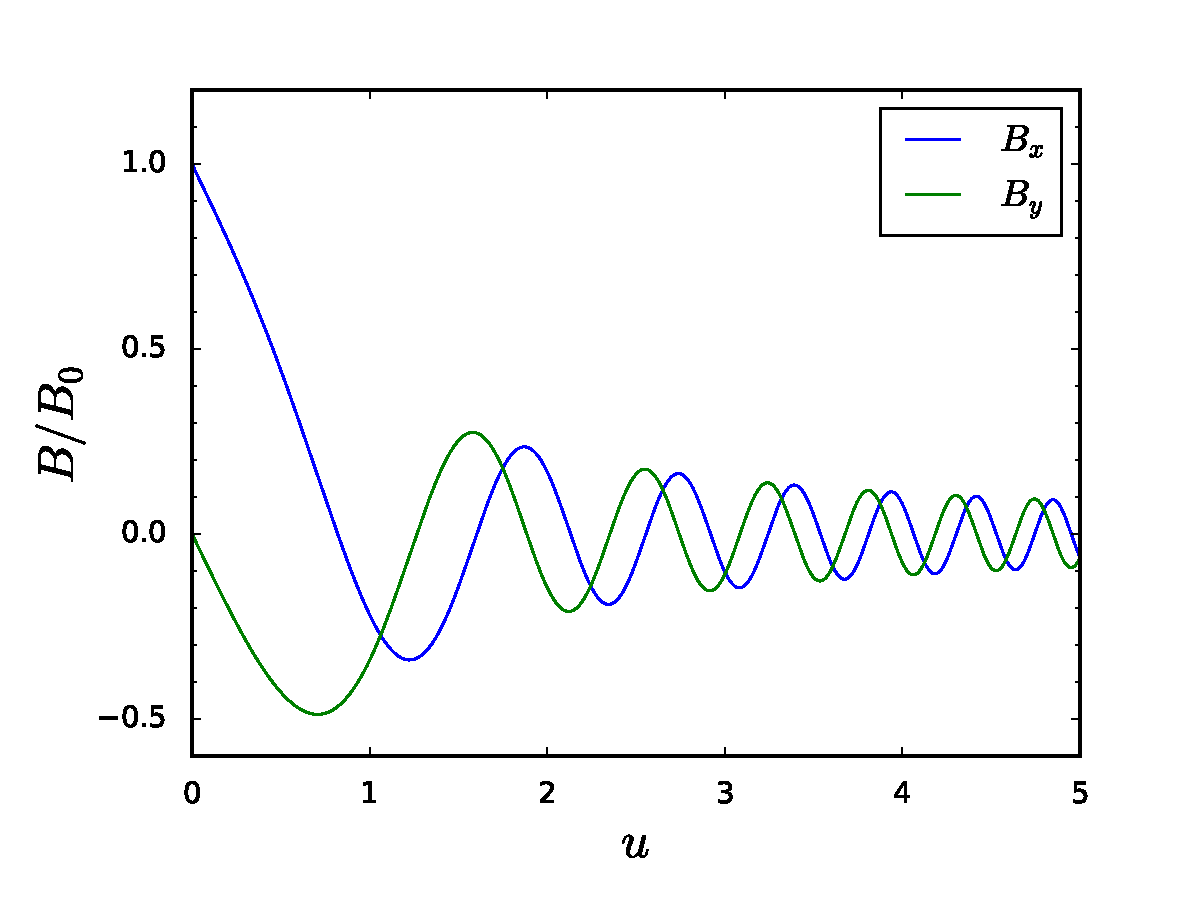
\includegraphics[width=0.6\textwidth]{pics/chap2/fresnel.pdf} 
\caption[Components of magnetic field in the self-similar solution of Hall waves]{
Self-similar wave $B_x(u)$, $B_y(u)$ (where $u = z/\sqrt{2D_H t}$) in a 
homogeneous crust of infinite conductivity with the initial $B=B_x+iB_y=0$. 
The wave is launched at $t=0$ and $z=0$ by the 
jump of $B_x$ from 0 to $B_0$.
$B_x=B_0$ is kept fixed at the boundary $z=0$ while the Hall evolution of 
$B(z,t)$ washes out the jump with time. The constant profile $B(u)$
implies the self-similar stretching of $B(z)$ as $z\propto t^{1/2}$, from initially
infinitesimal to arbitrary large widths.
}
\label{fresnel1}
\end{figure}
%%%%%%%%%%%%%%%%%%%%%%%%%%

Let us consider the initial condition $B(z,0)=0$ everywhere in the crust except
its boundary with the core, where the field jumps to $B_0\neq 0$. The boundary 
condition is fixed at $B_0$ throughout the evolution. Then the solution is given by
\begin{equation}\label{fre1}
  \frac{B(z,t)}{B_0} = 1-\sqrt{\frac{2}{\pi}}\frac{2}{1-i}\left[\mathcal{C}(u)-i\mathcal{S}(u)\right],
\end{equation}
where $u = z/\sqrt{4D_H t}$; $\mathcal{S}$ and $\mathcal{C}$ are Fresnel integrals,
\beq
	\mathcal{S}(u) = \int_0^u \sin(s^2)\:\md s,  \quad
	\mathcal{C}(u) = \int_0^u \cos(s^2)\:\md s.
\eeq
The solution is self-similar; its dependence on $u$ is shown in Figure~\ref{fresnel1}.
It demonstrates how the horizontal current sheet at the boundary generates a broad 
spectrum of Hall waves. The fast short waves lead the longer waves.

%%%%%%%%%%%%%%%%%%%%%%%%%%
\begin{figure*}[h]
\centering
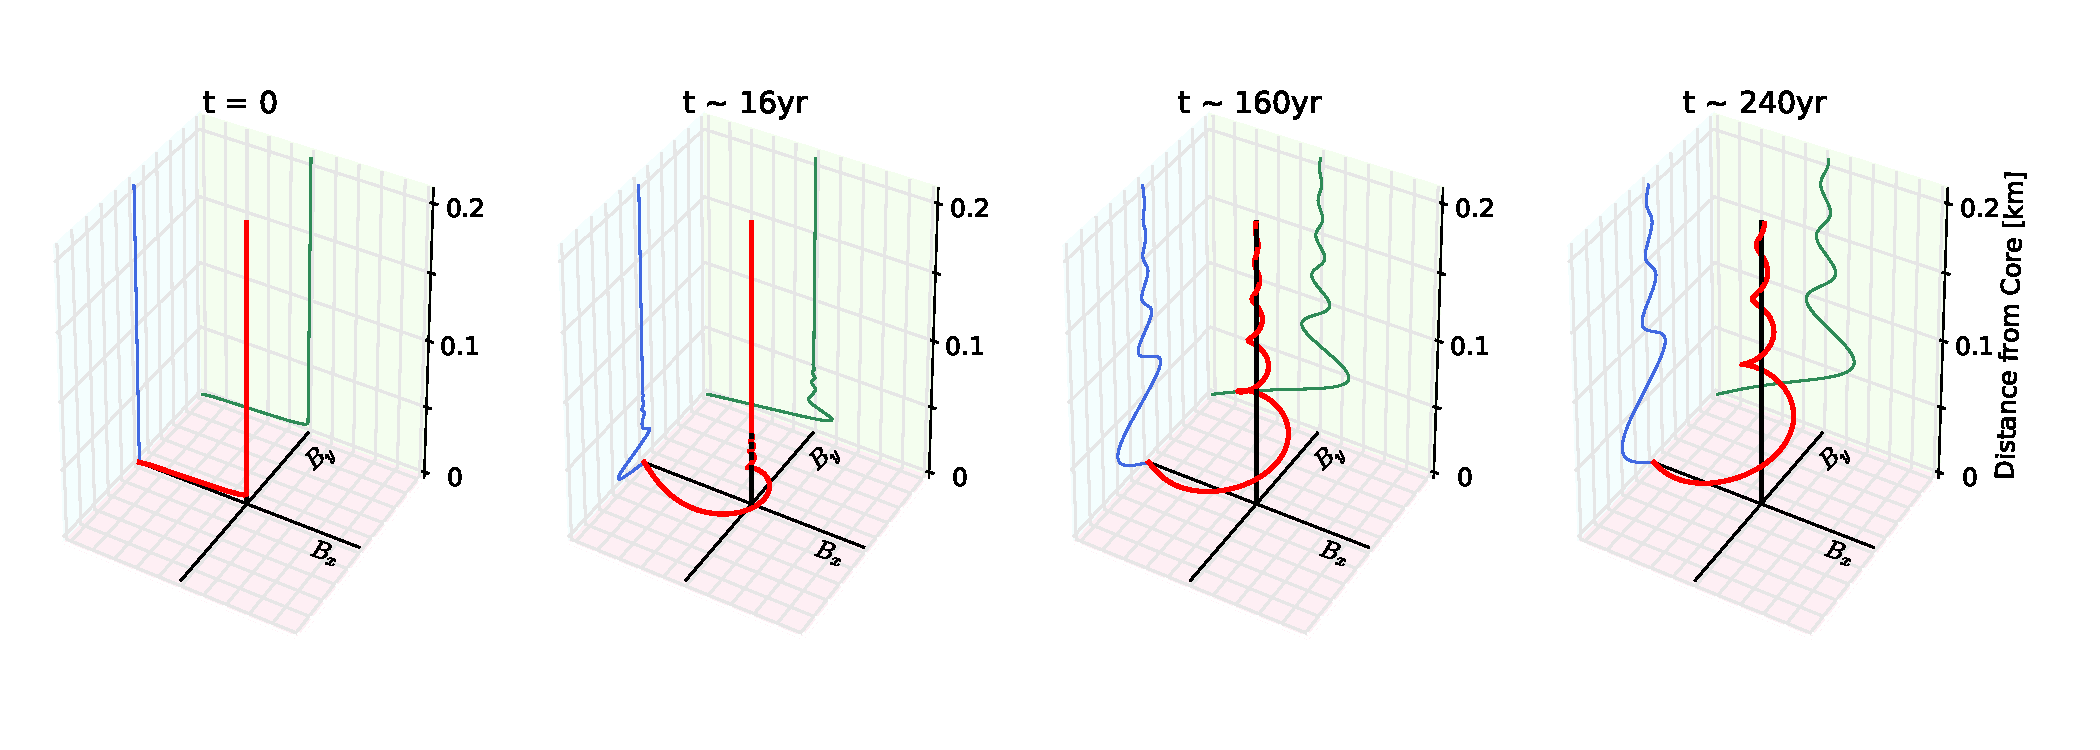
\includegraphics[width=1.0\textwidth]{pics/chap2/hall.pdf} 
\caption[Generation of Hall waves in the magnetar crust]{
Generation of Hall waves by a jump of $B_x$ from $B_x=0$ at $z\gtrsim 10$~m to 
$B_x=B_0=6\times 10^{15}$~G at $z=0$ (the core-crust interface). The four snapshots show 
the evolution of $B_x$ and $B_y$; vertical field $B_z=3\times 10^{14}$~G remains constant. 
The evolution is calculated using a realistic density profile $\rho(z)$ and conductivity 
$\sigma_{\rm el}(z)$ of the crust. The black lines indicate the $x,y,z$ axes.  The red curve traces 
the end of the horizontal vector $(B_x,B_y)$, which is a function of the vertical position $z$.
The green and blue projections show $B_x(z)$ and $B_y(z)$; they resemble the 
self-similar solution shown in Figure~\ref{fresnel1}.
}
\label{cartoon}
\end{figure*}
%%%%%%%%%%%%%%%%%%%%%%%%%%


The same problem with a realistic density profile $\rho(z)$ and electric conductivity 
$\gamma(z)$ can be solved numerically using \Eq~(\ref{hall}) (neglecting crustal 
deformation $\xi$). The finite resistivity leads to efficient damping of the fast Hall waves with 
high wavenumbers, limiting the speed of the wavefront launched by the jump of $B_x$.
Figure~\ref{cartoon} 
shows four snapshots of the resulting evolution of the magnetic field.

Similar waves will be launched by a plastic flow that has created a jump in $B$ at 
some $z_0>0$ inside the crust, as will be discussed below. In this case, one will need to 
trace the crustal Hall waves excited at $z<z_0$ and $z>z_0$.

\section{Plastic failures}\label{plastic}

\subsection{Stress balance}

Hall evolution can generate strong shear stresses $BB_z/4\pi$, where 
$B$ is the horizontal magnetic field.
As long as the external $B=0$ at the top of the crust (this assumption will be relaxed in 
Section \ref{twist}) the stress balance is only possible 
if the entire stress $BB_z/4\pi$ is offset by the elastic stress of the ion lattice,
\beq
\label{eq:stress}
   \frac{B B_z}{4\pi}=-\mu\,\partial_z \xi_{\rm ela}=\sigma,
\eeq
where $\mu$ is the shear modulus of the lattice. We expect the stress balance 
to be satisfied to a high precision at all times, even during a crustal failure when a plastic flow occurs \citep{2014ApJ...794L..24B}, provided that the plastic flow is slow compared with the relaxation to stress balance. The latter occurs on the shear-sound-crossing timescale $<$0.1~s. 

Taking the time derivative on both sides 
of \Eq~(\ref{eq:stress}) and substituting
into \Eq~(\ref{hall}), we get
 
\beq
\label{eq:evol}
\left(1+\frac{\mu_B}{\mu}\right)\dot{B}= -i\partial_z \left(D {\partial_z B} \right)+B_z\partial_z\dot{\xi}_{\rm pl},
\eeq
where $\mu_B\equiv B_z^2/4\pi$.
The above equation,
but without the plastic deformation term on the right-hand side, was derived 
and used to obtain the dispersion relation of  
Hall waves in \citet{2004ApJ...609..999C}. The elastic deformation of the crust strongly affects the Hall-wave propagation when $\mu<\mu_B$.

\subsection{Mechanical failure}\label{mechanical}


When the shear stress in the crust reaches a critical value 
\beq
\sigma_{\rm cr}\sim 0.1\mu,
\eeq
the crust must yield inelastically, as demonstrated in numerical experiments by 
\citet{2009PhRvL.102s1102H} and 
\citet{2010MNRAS.407L..54C}.
They propose that $\sigcr$ depends on temperature as
\beq\label{shearstress}
\sigma_{\rm cr}(T) = \sigma_{\rm cr}(0)\left(1-\frac{65.128}{\Gamma-71}\right), 
\eeq
where $\Gamma=Z^2 e^2/akT$ is the Coulomb coupling parameter for ions with charge
number $Z$ and separation $a=(3/4\pi n_{\rm i})^{1/3}$ ($n_{\rm i}$ is the ion number density.)
These authors studied rapidly shearing boxes of $\sim 100\times100\times 100$ lattice sites, 
and found that after the shear stress reaches $\sim 0.1\mu$ the failure develops with the 
stress reduced by an order of magnitude.
When the shear ends, the crystal strength must eventually heal.
Our model below will assume a similar behavior of the elastic stress in macroscopic
failure events, although the extrapolation of the small-scale rapid-shear experiments 
to slowly fostered macroscopic failures may not be reliable.
Note also that two-dimensional shear failures, common in the earth crust as sources of 
earthquakes, are strongly suppressed in a magnetar by magnetic tension 
\citep{2012MNRAS.427.1574L}. The failure may be described as 
a plastic flow \citep{2014ApJ...794L..24B}, see also \citet{2003ApJ...595..342J}.

The critical stress $\sigcr$ defines the critical magnetic field $\Bcr$,
\beq
  \frac{\Bcr B_z}{4\pi}=\sigcr.
\eeq
Motivated by the results of \citet{2009PhRvL.102s1102H}
we will
assume that once the failure
is initiated the critical stress  drops
to $\sigma_{\rm cr}^{\rm new}=0.1\sigma_{\rm cr}$. 
Correspondingly, $\Bcr^{\rm new}=0.1\Bcr$ during the plastic flow.
This prescription makes sure that the horizontal magnetic field evolves to the lower value $\Bcr^{\rm new}$ in a visco-elastic manner. Once the elastic stress reaches $\sigma_{\rm cr}^{\rm new}$ we assume that the lattice reforms and the visco-elastic evolution stops.
Our results are not sensitive to the exact choice of $\sigma_{\rm cr}$.

Finally, we specify the plastic flow rate (the last term in 
\Eq~(\ref{eq:evol})) using
a simple viscoelastic model,
\beq
B_z\partial_z \dot{\xi}_{\rm pl}=-\alpha B\left(1-\frac{B_{\rm cr}^{\rm new}}{|B|}\right)\Theta\left(|B|-B_{\rm cr}^{\rm new}\right).
\label{plasticprescription}
\eeq
Here $\Theta(...)$ is the Heaviside step function, so the plastic flow occurs as long as
$|B|>B_{\rm cr}^{\rm new}$. \Eq~(\ref{plasticprescription}) describes a shear failure motion 
that relaxes the local magnetic stress by driving the field $B$ from $\Bcr$ to $\Bcr^{\rm new}$.
The parameter $\alpha$ has the dimension of $s^{-1}$ and determines the relaxation rate.
After time $\tau\gg \alpha^{-1}$ from the beginning of the plastic failure, $B$ 
becomes exponentially close to $\Bcr^{\rm new}$ and the crystal should heal, i.e. the critical 
stress 
should increase
back to $\sigma_{\rm cr}\sim 0.1\mu$, ending the plastic flow. 
The qualitative results of this chapter were found to be weakly affected by the choice of rate 
$\alpha$ and healing time $\tau$ for reasonably fast plastic flow rates.
In the simulations presented below we use $\alpha=10^{-4}$~s$^{-1}$
and $\tau = 1$~yr.
 

\subsection{Heat transfer and thermoplastic waves}

The energy density that can be dissipated through plastic failures is 
the sum of magnetic and elastic energies,
\beq
 U = \frac{|B|^2}{8\pi}+\frac{1}{2}\mu |\partial_z \xi_{\rm ela}|^2 
 = \left(1+\frac{\mu_B}{\mu}\right)\frac{|B|^2}{8\pi}.
\eeq 
The dissipation rate due to plastic flow is given by
\begin{equation}
   q_{\rm pl}={B_z\left|B\partial_z \dot{\xi}_{\rm pl}\right|\over 4\pi},
\label{qpl}
\end{equation}
where $|B|=(B_x^2+B_y^2)^{1/2}$.

\citet{2014ApJ...794L..24B} showed that the temperature-softening effect,
i.e. the reduction of $\sigcr(T)$ with increasing $T$, allows the plastic failure to propagate through heat diffusion.
The resulting thermoplastic wave (TPW) resembles a deflagration front, and its speed is 
\beq
\label{eq:vTPW}
  v\sim(\alpha\chi)^{1/2},  
\eeq
where $\chi=\kappa/C_V\sim 10-100$~cm$^2$~s$^{-1}$
is the heat diffusion coefficient, 
with $C_V$ and $\kappa$ being the heat capacity and thermal conductivity of
the crustal
material.
The TPWs are much faster than the Hall waves, 
so the Hall evolution is negligible during the crustal failure through a TPW.

The TPW
propagation requires that
the magnetic field ahead of the wave $B_0$ 
be sufficiently close to $\Bcr$, so that heat diffusion from the plastic flow 
is capable of reducing
$\Bcr(T)$
below $B_0$. A simple propagating solution $B(z-vt)$ is obtained from 
\Eq~(\ref{plasticprescription}) assuming a uniform medium ahead of the wave with 
a uniform field $B_0$. Suppose the wave was launched at $z_\star$ at time $t_\star$.
In the plastically flowing region $z-vt<z_\star-vt_\star$,
\Eq~(\ref{plasticprescription}) gives
\beq
-v \frac{dB}{dw} = -\alpha B\left(1-\frac{\Bcr^{\rm new}}{|B|}\right), 
\qquad w=z-vt.
\eeq
Then one finds the solution,
\beq\label{tpw}
B = (B_0-B_1)\exp\left[\frac{\alpha}{v}(w-w_\star)\right]+B_0,  \quad w<w_\star,
\eeq 
which describes the plastic relaxation of $B_0$ to a weaker field $|B_1|=\Bcr^{\rm new}$.
One can see that the characteristic thickness of the wave front is $v/\alpha$.

A TPW launched in a non-uniform background will eventually extinguish, leaving 
a jump of the magnetic field $B_0\rightarrow B_1$ of width $\sim v/\alpha$. This jump affects the subsequent Hall evolution of the magnetic field.

\section{Hall-mediated avalanche}\label{avalanche}

The jumps of the horizontal magnetic field as a result of plastic failures generate Hall waves.
This can be illustrated by an idealized model of a homogeneous crust with an initially uniform field $B_0$ that was suddenly changed to $B_1=0.1B_0$ at $z<z_0$. 
$|B_1|=\Bcr^{\rm new}$ carries the same meaning as in Equation (\ref{tpw}).
The problem is similar to that considered in Section~\ref{dyn} except that now $B$ jumps from $B_0$ to $B_1$ at $z_0$ instead of jumping from $B_0$ to $0$ at $z=0$.

The analytical solution for the Hall evolution caused by the jump is given by
\begin{equation}\label{fre2}
B(z,t)=B_1+ \frac{(8/\pi)^{1/2}}{1-i}\left[\mathcal{C}(u)-i\mathcal{S}(u)\right](B_0-B_1),
\end{equation}
where $u = (z-z_0)/\sqrt{4D_H (t-t_0)}$ and $t_0$ is the initial time at which the jump was created. 
Snapshots of this solution at $z>z_0$ are shown in Figure~\ref{fresnel2}.
This solution is similar to Equation (\ref{fre1}), but with different boundary conditions.
The peaks of the oscillating profile are moving from left to right and their widths increase with time as $t^{1/2}$. 
In the idealized problem, where the infinitely sharp jump is created instantaneously, the peaks start out infinitesimally narrow.
More realistically, the jump is implanted at the end of a plastic failure in a finite time $\delta t\sim \alpha^{-1}$. This timescale determines the characteristic peak width at the beginning of the evolution. 
At times $t-t_0\gg\delta t$ the evolution becomes self-similar and accurately described by \Eq~(\ref{fre2}).

%%%%%%%%%%%%%%%%%%%%%%%%%%
\begin{figure}[h]
\centering
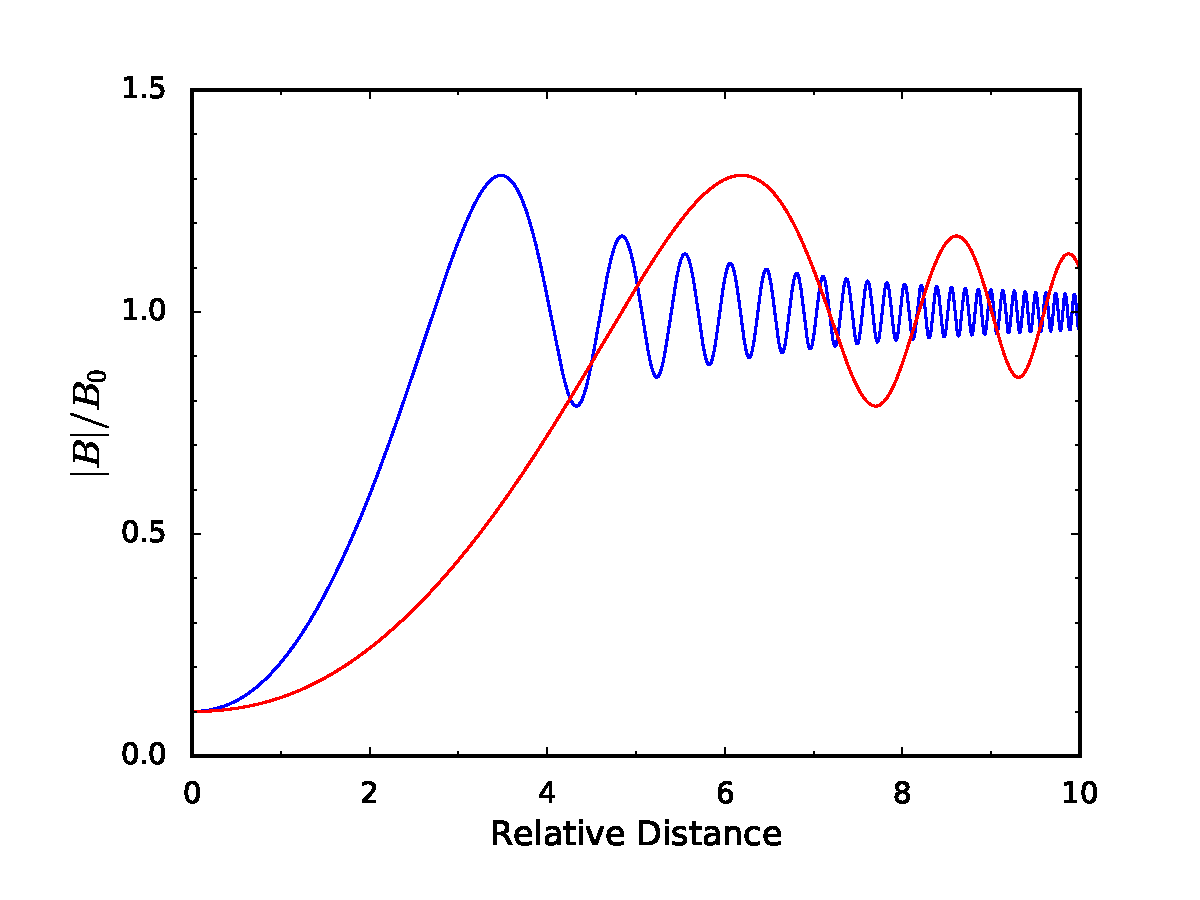
\includegraphics[width=0.6\textwidth]{pics/chap2/fresnel2.pdf} 
\caption[Profile of the horizontal magnetic field]{Profile of the horizontal magnetic field $|B|$ at two different times,
according to the self-similar solution given by \Eq~(\ref{fre2}). The peaks are
moving from left to right.}
\label{fresnel2}
\end{figure}
%%%%%%%%%%%%%%%%%%%%%%%%%%

A key feature is that {\it the peaks of the launched Hall waves significantly exceed 
the background field $B_0$}. 
The highest peak is $1.3B_0$. This implies that the Hall waves 
are capable of breaking the crust and inducing new plastic flows, leading to an avalanche
of plastic failures.
\footnote{While we believe that this effect will also be present in multi-dimensional configurations, geometry and non-linearities present in multi-dimension can change it quantitatively}

The avalanche development can be demonstrated by the following numerical experiment.
Consider a uniform crust with electron density $n_e = 10^{35}$~cm$^{-3}$ and 
$B_z=3\times 10^{14}$~G; this gives the Hall diffusion coefficient 
$D_H \approx 0.015$~cm$^2$~s$^{-1}$.
To isolate the effect of interest we turn off heat diffusion, so there will be no TPWs, 
and new plastic flows can only be induced by Hall waves. As an initial condition at $t=0$ 
we take a uniform field $|B_0|=2.7\times 10^{14}$~G. We set 
$\Bcr= 3\times 10^{14}$~G everywhere except a small region $|z-z_0|<2$~m. 
In this region, we trigger the plastic flow by setting $\Bcr^{\rm new}=0.1\Bcr$. 
This setup is designed to produce an initially localized plastic flow, which 
reduces the field in the small region and launches Hall waves. Our experiment follows the evolution
by solving the Hall equation (\ref{eq:evol})  and simulating any new plastic flows, which must be
triggered wherever $|B|$ exceeds $\Bcr$.

%%%%%%%%%%%%%%%%%%%%%%%%%%
\begin{figure}[h]
\centering
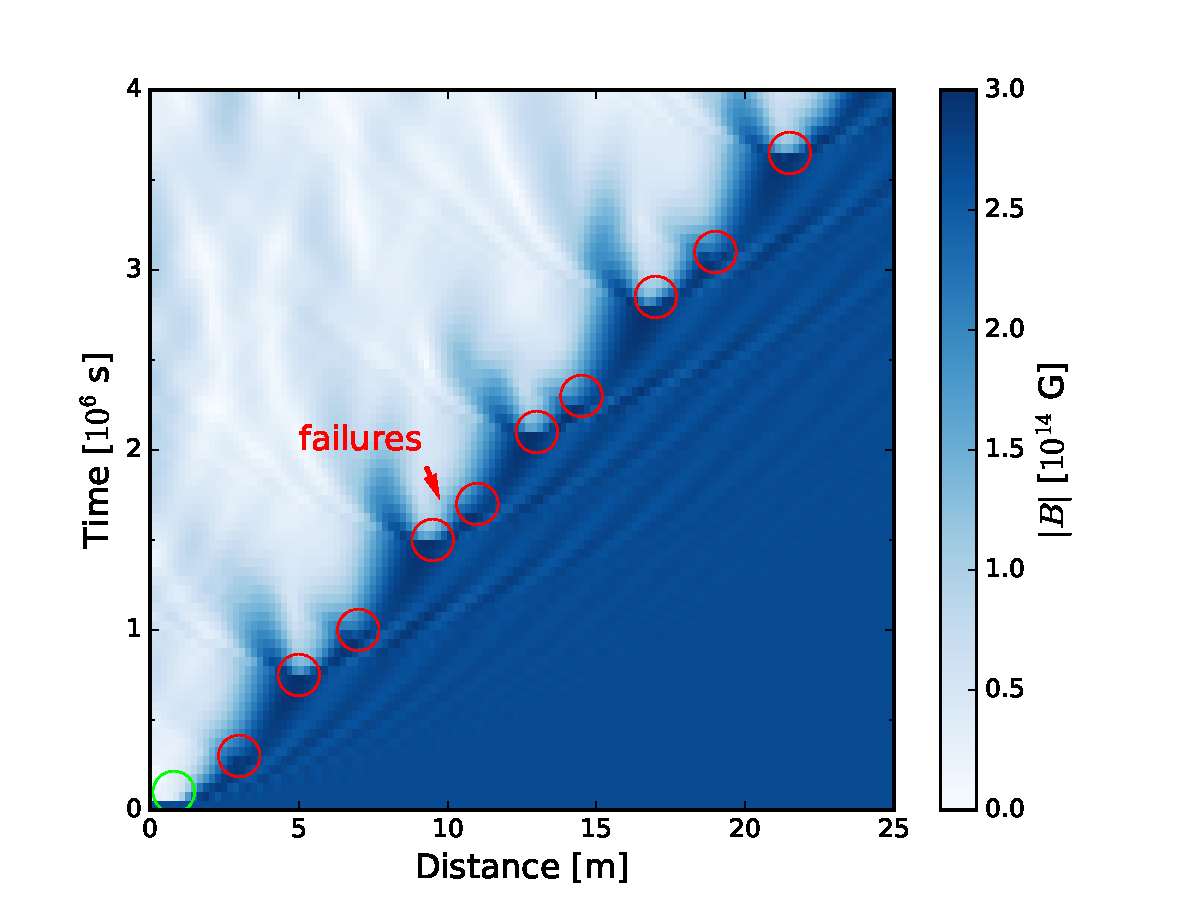
\includegraphics[width=0.6\textwidth]{pics/chap2/failure.pdf} 
\caption[Numerical simulation demonstrating the Hall-mediated failure of the crust]{
Numerical simulation demonstrating the Hall-mediated failure of the crust
(see text). A seed plastic failure
is initiated at $t=0$ and $z<2$~m; it is indicated by the green circle on the spacetime 
diagram. Magnetic field $|B|$ is quickly reduced in the failed region, so it becomes 
white (weak field) according to the color code indicated next to the diagram. 
The failed region is expanding due to the short Hall waves launched
by the plastic flows into the intact region, 
where the waves trigger new plastic flows.
}
\label{failure}
\end{figure}
%%%%%%%%%%%%%%%%%%%%%%%%%%

The result is convenient to view on the spacetime digram (Figure~\ref{failure}) that shows the 
evolution of $|B|$ in the region $z>z_0$. As expected, the peaks of launched Hall waves 
break the crust, creating new plastic flows. These flows generate new jumps in $B$, which 
create new Hall waves etc., expanding the region where the crust has failed. 
The average speed of the failed region expansion is determined by the slope 
of the boundary $z_{\rm front}\approx vt$ observed on the diagram. The magnetic field 
$|B|$ has been reduced (and magnetic energy has been dissipated) in the region 
$z<z_{\rm front}$. In contrast, in the region $z>z_{\rm front}$, the field is only perturbed by the faster and weaker 
Hall waves, which are seen as the propagating oscillations. 
The front speed is $v\approx 5.5\times 10^{-4}$~cm/s, about half of 
$(\alpha D_H)^{1/2}=1.2\times 10^{-3}$~cm/s --- the characteristic speed of
Hall waves launched by plastic flows. As a rough estimate one can use
\beq
\label{eq:vH}
  v\sim (\alpha D_H)^{1/2}.
\eeq
In essence, we observe a {\it Hall-mediated mode of crustal failure} (HMF). 
It is much slower than the heat-mediated TPW, however it can operate where 
TPWs do not propagate.

The HMF expansion occurs with 
no clean separation of the timescales of Hall and 
plastic evolution --- the frequencies of excited Hall waves are comparable to $\alpha^{-1}$.
Therefore, the details of failure propagation are complicated. In particular, we 
observe a curious limit-cycle behavior:
a fast reduction of $|B|$ on the timescale $\alpha^{-1}$ is followed by a failure
event with a slower reduction of $|B|$ in a smaller region; then it takes a long 
time to trigger a new failure which again turns out fast and strong, closing the cycle.

The cycle is explained as follows. A fast failure launches a Hall wave with
a narrow peak, $\delta z\sim (D_H/\alpha)^{1/2}$, and therefore the next plastic 
flow triggered by this peak occurs promptly and in a narrow region.\footnote{Plastic 
     flow is initiated where the growing peak touches $\Bcr$, and the width of the induced 
     failure is controlled by the curvature of $|B(z)|$ at the peak.
     In a complete model, with heat diffusion,
     a local TPW is produced, which quickly extinguishes as it propagates
     away from the peak. The model with switched off heat diffusion does not generate TPWs; 
     instead, it generates a cascade of very thin plastic flows (limited by the grid resolution of
     $2$~cm), which merge with time. Thus, the behavior on the smallest scales cannot be 
     resolved in the simulation presented in Figure~4. However, the small-scale details weakly 
     affect the behavior
     of the front on scales well above the grid scale --- it turns out similar to 
     a more complete simulation with included heat diffusion.
     }    
The relaxation of $|B|$ to $\Bcr^{\rm new}=0.1\Bcr$ in the narrow plastic region
is hindered by the Hall-wave transport of magnetic energy
--- the locally dissipated magnetic energy is replenished 
by the Poynting flux 
\begin{eqnarray}
F_p&=&\frac{1}{8\pi} i D_H(B^*\partial_z B-B\partial_z B^*) \nonumber\\
 &=&\frac{1}{4\pi}D_H(B_y\partial_z B_x-B_x\partial_z B_y)
\end{eqnarray}
into the plastic region, which resists the development of a localized
sharp drop in $|B|$.
The delay in the drop of $|B|$ causes a delay in the launching of a new super-critical 
Hall wave into the intact region ahead of $z_{\rm front}$.
As a result the next failure event at $z>z_{\rm front}$ is 
delayed. When it finally occurs the wave peak is broad and triggers a plastic flow in a 
relatively broad region.  The relaxation $|B|\rightarrow \Bcr^{\rm new}$ in the broad 
region is not hindered by the Poynting flux and occurs promptly, on the timescale of 
$\sim \alpha^{-1}$.

The limit cycle can be clearly seen in
Figure~\ref{failure} as the repeating appearance of ``fingers'' and fast failures.
A ``finger'' pattern (e.g. one near distance $4$~m and time $10^6$~s) contains narrow failures separated by intact regions. 
Magnetic energy is only dissipated at narrow failure sites,
and the Poynting flux from intact regions 
replenishes the energy there.
It takes longer for $|B|$ to drop below $B_{\rm cr}^{\rm new}$ in the ``finger'' compared to fast failures to the right.
After a fast failure in a broad region, new narrow failures are reproduced. Therefore the ``finger'' appears again.

We also performed simulations similar to that shown in Figure~\ref{failure} that included 
heat diffusion and ohmic dissipation with a realistic $\eta\sim D_H/20$. 
We observed a similar propagation of the failure front, but with gradually damped peaks of the Hall waves. 
We also varied $|B_0|/\Bcr$ and found that when this ratio is closer to unity, the TPW becomes the dominant mode of failure propagation. 
It propagates much faster, with the velocity $v_{\rm TPW}\sim (\alpha\chi)^{1/2}$ well above the velocity of the Hall-mediated failure $v_{\rm HMF} \sim(\alpha D_H)^{1/2}$.
Both failure modes will be seen to occur in the magnetar crust simulated in Section~\ref{sim}.

\section{Twisted external field}
\label{twist}

The crustal motions must twist the external magnetosphere attached to the crust. 
Such external twists are observed in persistent magnetars through their hard X-ray emission \citep{2013ApJ...762...13B, 2014ApJ...786L...1H}.
In transient magnetars, evidence for magnetospheric twists is provided by shrinking hot spots on the stellar surface \citep{2009ApJ...703.1044B}.

The external twist implies a non-zero horizontal magnetic field at the stellar surface $B_s\neq 0$. 
This changes the stress balance inside the crust, which now reads
\beq
   \frac{\tilde{B} B_z}{4\pi}=-\mu\partial_z \xi_{\rm ela}, \qquad \tilde{B}=B-B_s.
\eeq
It leads to a modified version of \Eq~(\ref{eq:evol}) for the magnetic field evolution, 
\beq\label{fulleqn}
\left(1+\frac{\mu_B}{\mu}\right)\dot{B}= -i\partial_z\left(D\partial_z B \right)+\frac{B_z^2}{4\pi\mu}\dot{B_s}+B_z\partial_z\dot{\xi}_{\rm pl}.
\eeq
Plastic flows are triggered where $\tilde{B}$ exceeds $\Bcr$, and $\tilde{B}$ should replace $B$ in the equation of plastic flow dynamics. 
Therefore, \Eq~(\ref{plasticprescription}) is replaced by
\beq
B_z\partial_z \dot{\xi}_{\rm pl}=-\alpha \tilde{B}\left(1-\frac{B_{\rm cr}^{\rm new}}{|\tilde{B}|}\right)\Theta\left(|\tilde{B}|-B_{\rm cr}^{\rm new}\right).
\label{plasticprescription1}
\eeq

To close the set of equations describing the system, one must specify the evolution of $B_s$. 
It is controlled by two factors: 
(1) $B_s$ is pumped by the crustal motions.
(2) The external twist has a finite lifetime, because it requires a magnetospheric current ${\mathbf j}=(c/4\pi)\nabla\times{\mathbf B}\neq 0$. 
For instance, in the axisymmetric geometry $B_s\neq 0$ would be a toroidal field which requires a poloidal magnetospheric current \citep{2002ApJ...574..332T}. 
The current is sustained through $e^\pm$ discharge with a threshold voltage that regulates the damping time of the external twist to $\sim 1$~yr \citep{2007ApJ...657..967B}.

The pumping of $B_s$ by crustal motions can be implemented in our one-dimensional model as shown in Figure \ref{fig1}.
We consider a magnetosphere with a constant vertical magnetic field $B_z$ and a constant horizontal field $B_s$ that serves as a proxy for the twist component in three dimensions.
The pumping of $B_s$ is caused by the motion of magnetic field lines at the crust surface. 
This motion can be related to the evolution of $B(z,t)$ inside the crust by integrating \Eq~(\ref{vel}) from the bottom to the top of the crust,

\beq
\int\limits_{\rm bottom}^{\rm surface}\md z\,\left.\frac{\dot{B}}{B_z}=(v+\eta\partial_z B)\right|_{\rm bottom}^{\rm surface},
\eeq
where $v(z,t)=v_H+\dot{\xi}=v_x+iv_y$ is the velocity vector of the electron fluid. 
Neglecting the lattice deformation at the base of the crust, 
$\dot{\xi}_{\rm bottom}=0$, we get the surface velocity of the magnetic field lines,
\beq
v_s=\int\limits_{\rm bottom}^{\rm surface}\md z\,\frac{\dot{B}}{B_z}
+\left(v_H+\eta\partial_z B\right)_{\rm bottom}.
\label{vsurf}
\eeq
Here we kept the resistive term $\eta\partial_z B$ at the bottom (because the typical setup of our simulations has a strong current sheet at the bottom), and neglected $\eta\partial_z B$ at the surface, as its effect on the evolution of $B_s$ will be small compared to ohmic dissipation in the magnetosphere.
The magnetic field at the surface follows the motion of the electron fluid with velocity $v_s$.

The rate of pumping $B_s$ is proportional to $v_s$, and the evolution equation for $B_s$ may be written in the form,
\beq\label{bs}
\dot{B}_s=-B_z\frac{v_s}{L}-\frac{B_s}{\tau_{\rm damp}}.
\eeq
Here $L$ represents the length of the magnetospheric field lines (Figure~\ref{fig1}) and $\tau_{\rm damp}$ is the damping timescale. 
In a complete model, the value of $\tau_{\rm damp}$ would depend on the voltage of $e^\pm$ discharge in the magnetosphere and the geometry of the twisted bundle of field lines \citep{2009ApJ...703.1044B}.  
In our simplified model we fix $\tau_{\rm damp}=1$~yr.

The Hall evolution at the bottom boundary is slow and not capable of pumping 
$B_s$ against the twist damping in the magnetosphere. 
However, significant external twists can 
be created as a result of the large $\dot{B}$ in the regions of plastic 
failures \citep{2014ApJ...794L..24B}. 

%%%%%%%%%%%%%%%%%%%%%%%%%%
\begin{figure}[t]
\centering
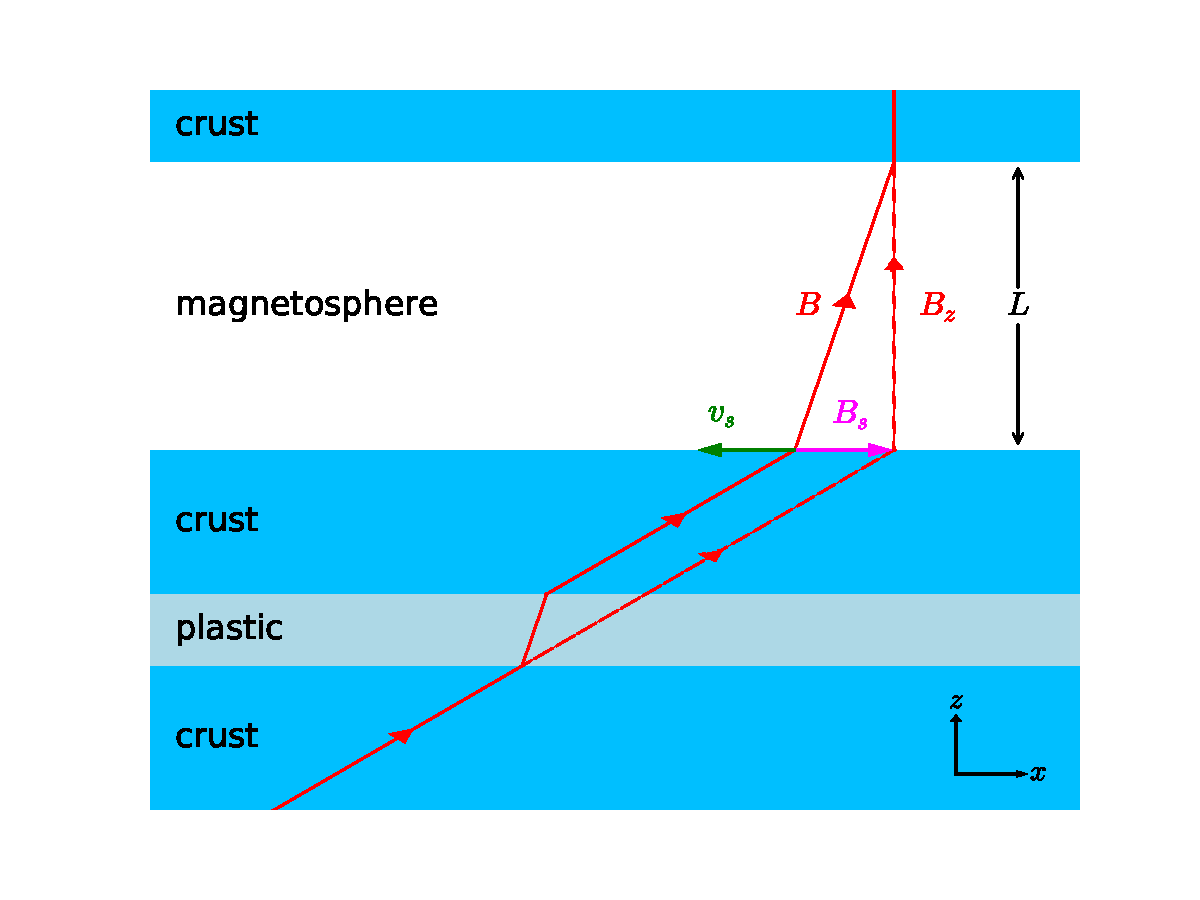
\includegraphics[width=0.6\textwidth]{pics/chap2/twist.pdf} 
\caption[Illustration for the magnetic field lines in the crust and in the 
magnetosphere]{Illustration for the magnetic field lines in the crust (blue region) and in the 
magnetosphere (white region). 
A closed magnetic field line is anchored between two footpoints in the crust. The plot is projected in the direction of magnetic field line.
Plastic flow 
occurs
in the light blue region and 
results in a crustal surface motion
with velocity $v_s$. This motion shears the magnetosphere 
and creates $B_s$.
Red dashed and solid lines are the magnetic field line before and after 
the plastic deformation. 
}
\label{fig1}
\end{figure}
%%%%%%%%%%%%%%%%%%%%%%%%%%

\section{Global Simulation}
\label{sim}

\subsection{Setup}

We now collect all the ingredients described in the previous sections into a 
global simulation of the magnetic field evolution in a magnetar crust over $10$~kyr.
The crust will now have a realistic density profile $\rho(z)$. Its temperature profile $T(z)$ is calculated self-consistently by evolving the time-dependent equation for heat transfer,
\beq\label{heat}
 C_V\dot{T}=\partial_z\left(\kappa \partial_z T\right)+q_{\rm pl}+q_{\rm ohm}-q_{\nu}.
 \eeq
It takes into account the plastic heating (\Eq~\ref{qpl}), the ohmic heating $q_{\rm ohm}=(\eta/4\pi)|\partial_zB|^2$, and the energy losses due to neutrino emission $q_\nu$.

The coupled evolution of $B(z,t)$ and $T(z,t)$ in the crust, and $B_s(t)$ at the surface, is followed by solving Equations~(\ref{fulleqn}), (\ref{heat}), (\ref{vsurf}), and (\ref{bs}); \Eq~(\ref{plasticprescription1}) is used where plastic flows occur.

While our one-dimensional model can only approximate the behaviour of a real magnetar, it allows one to use a realistic vertical profile for all of the important physical parameters of the crust.
We use the BSK20 model provided by \citet{2013A&A...560A..48P} to compute the density $\rho$, electron number density $n_e$, nuclear charge $Z$ and mass $A$ as a function of depth $z$. 
The mass  of the neutron star is chosen to be $1.4M_{\odot}$, for which the model predicts the radius of  11.7~km.
The shear modulus $\mu$ is calculated using the fitting formula provided by \citet{2005ApJ...634L.153P} and \citet{2007MNRAS.375..261S} for low and high densities. 
To accelerate the computations, in most of our runs the ohmic diffusivity  is set to $\eta = |D_H|/20$, the value which is characteristic for the inner crust. We have separately checked that the details of ohmic dissipation do not affect our results, as most of the energy is dissipated in the plastic flow regions.  
Our fiducial value for the vertical magnetic field is $B_z = 3\times 10^{14}$~G, which is a typical poloidal field of magnetars inferred from their spindown rates.

We choose the upper boundary of our simulation domain at $z=z_b$ where $\rho_b\equiv\rho(z_b)=10^{9}$~g/cm$^3$. 
Our results are not sensitive to this choice so long as 
(1) the crustal shear modulus at the boundary is sufficiently weak, $\mu(\rho_b)\ll B_z^2/4\pi$, and (2) the timescale of heat conduction from the boundary to the stellar surface $t_c(\rho_b)$ is much shorter than the typical conduction time across the crust, which is comparable to one year. 
The choice of $\rho_b=10^9$~g/cm$^3$ gives $4\pi\mu(\rho_b)/B_z^2\sim 10^{-4}$ and $t_c(\rho_b)\sim 10^6$~s for typical magnetar temperatures. 
Our computational box includes the entire crust at $\rho>\rho_b$, which has a
thickness of about 1~km. 
We use $30,000$ evenly spaced grid points; this gives enough resolution for capturing small-scale Hall waves.

We employ the Crank-Nicolson scheme \citep{press2007numerical} to solve both the Hall wave propagation and the thermal evolution.
In our fiducial run, we keep a constant horizontal magnetic field $B_{\rm core}=6\times 10^{15}$~G at the lower crust boundary $z_{\rm core}$. The horizontal field at the upper boundary $B_s$ evolves dynamically according to \Eq~(\ref{bs}), which provides a time-dependent boundary condition at $\rho_b$. 
The initial condition for the horizontal field $B$ is chosen to be
\beq
B(z)=B_{\rm core}\exp\left[-\frac{(z-z_{\rm core})^2}{l^2} \right],
\qquad z_b<z<z_{\rm core},
\eeq
with $l=10$~m. 
Thus, initially the crust has practically no horizontal field, and the presence of a strong horizontal field at the boundary launches Hall waves into the crust as 
described in Section~\ref{generation}.
The exact value of $l\ll 100$~m has no impact on the model's long-term behavior. 
We envisage that this type of initial configuration may result from a quick rearrangement of the core magnetic field.

It is important for our purposes to accurately track the thermal evolution of the crust. 
We choose the initial surface temperature to be $T_{s0}=2\times 10^6$~K which is typical for transient magnetars in quiescence.
The initial temperature profile below the surface sustains the steady heat flux $F=-\kappa\partial_z T=\sigma_{\rm SB} T_{s0}^4$ conducted from the core. 
The corresponding temperature of the core and the lower crust is $\sim 3\times 10^8$~K.
Neutrino cooling is negligible at such temperatures, however it becomes important later when the crust is heated by the avalanches of Hall waves and thermoplastic waves. 
For simplicity, the core temperature is kept constant throughout the simulation.
This may be reasonable due to the high heat capacity of the core, and this also
assumes that the main phase of its intrinsic thermal evolution occurred at 
earlier times, see \citet{2016ApJ...833..261B}.
The temperature profile of the heated crust is evolved by solving the time-dependent heat transfer equation as described in \citet{2015ApJ...815...25L}.
We use the code provided by \citet{1999A&A...351..787P} to calculate $C_V$ and $\kappa$ in the strong magnetic field. 
At high temperatures, the crust is efficiently cooled by neutrino emission.
Several processes contribute to the neutrino emissivity $q_\nu$; our simulations include the effects of annihilation of electron-positron pairs, plasmon decay, neutrino bremsstrahlung, and neutrino synchrotron emission. We use the formulae provided in \citet{2001PhR...354....1Y} to calculate $q_\nu$ from all these channels. 

The Hall wave propagation is typically slow compared to plastic instabilities and heat propagation. 
Therefore, the timestep in our simulations is adaptive and chosen to resolve the fastest processes when they happen --- the plastic flows, neutrino cooling, and twisting of the external magnetosphere. 
We require that the local temperature change due to plastic heating or neutrino emission in one timestep does not exceed $10^7$~K and the change in $B_s$ is smaller than $10^{9}$~G. 
To speed up the calculation, we track the thermal evolution only when there is an episode of plastic heating until the temperature profile has relaxed back to the steady heat flow from the core (i.e. when the temperature profile is everywhere close to the initial state, with deviations smaller than $10^7$~K). 
When the thermal evolution is turned off, the timestep is set at $5\times 10^4$~s. 
We have tested that it is short enough to resolve the Hall wave propagation in the absence of plastic failures. 
We use $\alpha= 10^{-4}$~s$^{-1}$ and run our simulation to 10~kyr. 
The energy conservation is better than 1\% during the whole simulation for Hall wave evolution and 5\% for thermal evolution.


When no plastic failure is triggered, the crust is only heated by ohmic dissipation.
Its effect on temperature is however small, $\Delta T<10^7$~K. When a plastic failure occurs, the local plastic heating greatly exceeds the ohmic heating. 
Therefore, we neglect the contribution of ohmic heating in the thermal evolution equation at all times. 
However, ohmic damping is taken into account in the Hall evolution equation for the magnetic field, where its effect is more significant.

As explained in Section~\ref{plastic}, an important element of our model is the dependence of the critical shear stress on temperature (the thermal softening of the crust). 
We use the expression given in \Eq~(\ref{shearstress}) as long as there is no plastic failure. When the plastic flow is initiated, at failed sites the maximal shear stress supported by the crust drops to $\sigcr^{\rm new}$, 10\% of its original value at zero temperature; this corresponds to the reduction of $\Bcr$ by a factor of 10 (see Section~\ref{mechanical}).
The crustal lattice heals when $|B-B_s|B_z/4\pi$ approaches $\sigcr^{\rm new}$, which occurs on the timescale of $3000/\alpha\sim 1$~year. At this point, the critical shear stress is increased back to the value given by \Eq~(\ref{shearstress}).
If the strong local heating melts the crust, then $\sigcr$ vanishes and the local $B$ must immediately relax to $B_s$, releasing magnetic energy. 
The dynamics of this fast process is not resolved in our simulations, instead we simply allow $B-B_s$ to be exponentially reduced on the timescale $\alpha^{-1}$ and convert the released magnetic energy to heat.

%%%%%%%%%%%%%%%%%%%%%%%%%%
\begin{figure}[htbp]
\centering
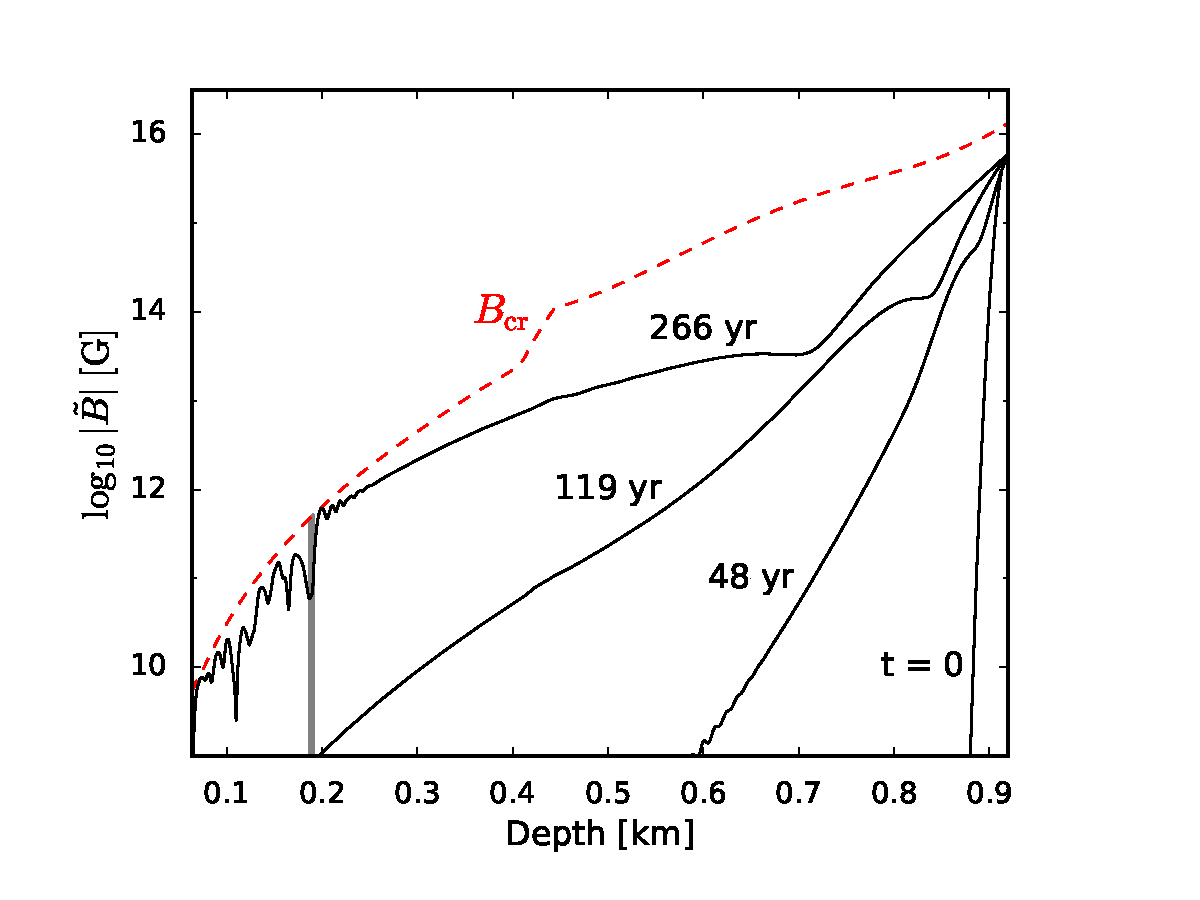
\includegraphics[width=0.6\textwidth]{pics/chap2/fig2.pdf} 
\caption[Snapshots of
the magnetic field evolution]{Snapshots of the magnetic field evolution, showing how the horizontal magnetic field $B$ gradually fills the crust from its lower boundary at $z\approx 1$~km. 
$\Bcr$ is calculated at the steady-state temperature profile that corresponds to the surface temperature of $2\times 10^{6}$~K.}
\label{fig2}
\end{figure}
%%%%%%%%%%%%%%%%%%%%%%%%%%

\subsection{Results}


Figure~\ref{fig2} shows the initial Hall evolution, which gradually fills the crust with a horizontal magnetic field. 
The horizontal axis shows the depth of the crust. The neutron star surface is to the left and core-crust interface is on the right where Hall waves are launched.
Solid curves show $|\tilde{B}|=|B-B_s|$ vs. depth $z$. 
$B_s\neq 0$ corresponds to the external magnetospheric twist; it is negligible at most times, except when the magnetosphere is quickly twisted by the plastic 
instabilities of the crust. 
Such motions are triggered when $\tilde{B}$ approaches $\Bcr$ (shown by the dashed red curve). 
This is seen to happen in the snapshot at $t=266$~yr; the plastically flowing region at $z\sim 0.2$~km is indicated by the vertical grey strip.
New Hall waves are launched from the plastic failures, and then the evolution continues in a chaotic manner, with repeating thermoplastic waves and Hall-mediated avalanches at various locations in the crust.

%%%%%%%%%%%%%%%%%%%%%%%%%%
\begin{figure*}[htbp]
\centering
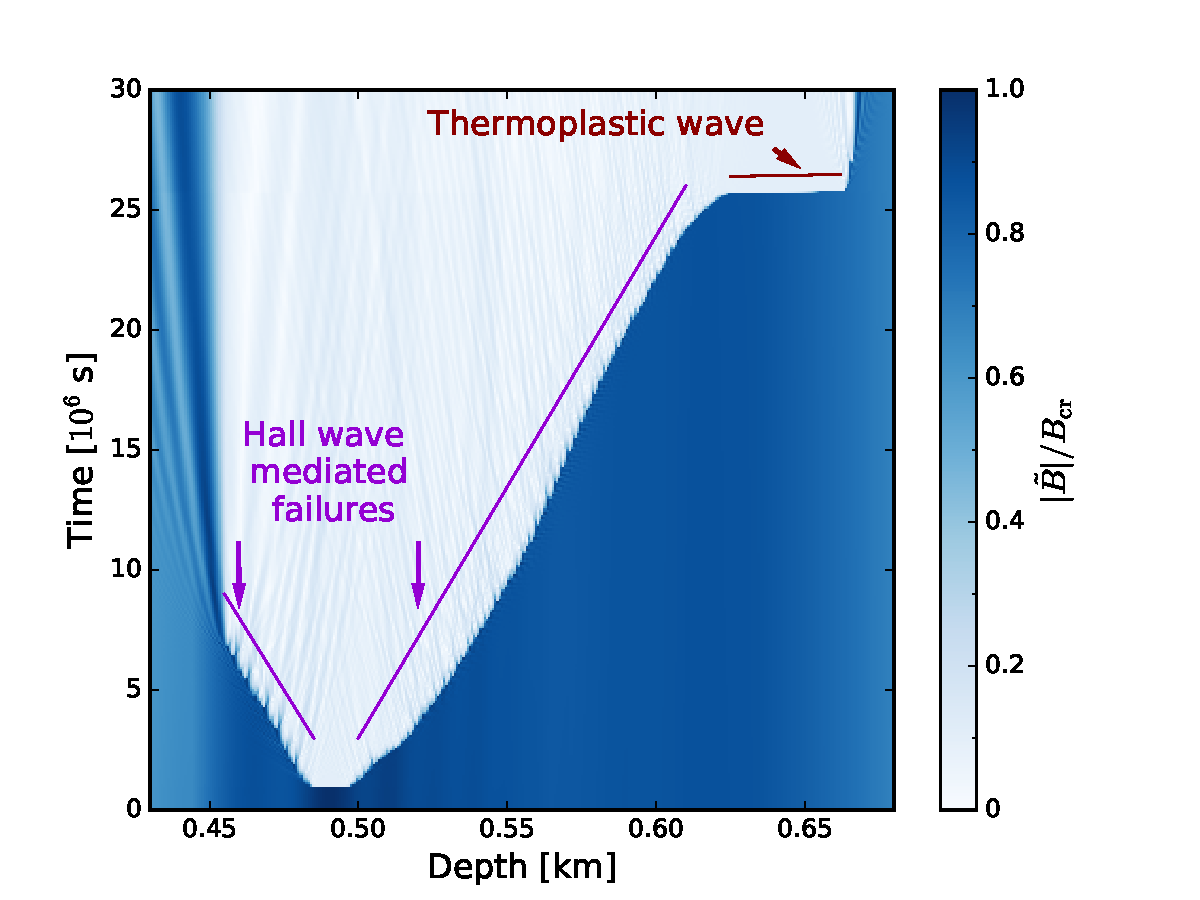
\includegraphics[width=0.48\textwidth]{pics/chap2/sp2.pdf}
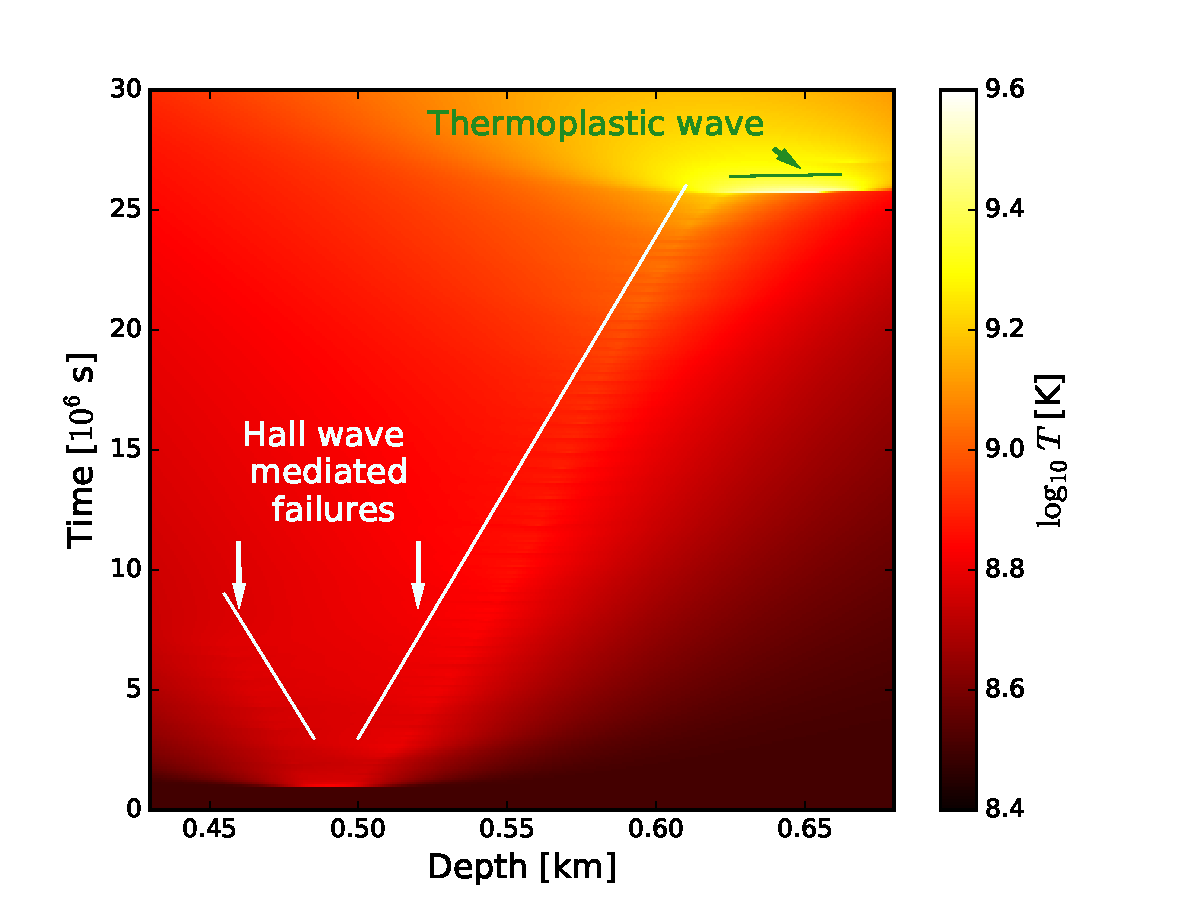
\includegraphics[width=0.48\textwidth]{pics/chap2/sp2_1.pdf} 

\caption[Spacetime diagram for failure generation and propagation in the crust]{Spacetime diagram for failure generation and propagation in the crust. 
\textbf{Left panel:} evolution of $|\tilde{B}|/B_{\rm cr}$.
At the failure sites, the value of $|\tilde{B}|/B_{\rm cr}$ drops to 0.1 which 
corresponds to the pale blue color.
The magnetic stresses in the neighborhood of the first failures (which are about 20~m thick) are not able to launch large thermoplastic waves. Instead, propagation of the initial failures is assisted by short Hall waves.
When the Hall-mediated avalanche reaches the depth of 0.6~km, a strong thermoplastic wave is launched, which propagates much faster and quickly reaches $z\approx 0.67$~km, where the wave extinguishes.
\textbf{Right panel}: 
Temperature evolution. Before the failure is triggered 
the temperature is kept near the initial steady state. 
As the failure develops, plastic heating increases the temperature. The heating is particularly strong in the thermoplastic wave developing at $z\approx 0.6$~km.
}
\label{sp2}
\end{figure*}
%%%%%%%%%%%%%%%%%%%%%%%%%%

The spacetime diagram in Figure~\ref{sp2} shows failure development during a major 
Hall-mediated avalanche at $z\approx 0.5$~km, which propagates into the deeper crust and concludes with a strong thermoplastic wave at $z=0.6-0.67$~km.
The duration of the avalanche is about one year.
A significant magnetic and elastic energy is dissipated during this time through the friction in the plastic flow (crustal ohmic heating makes a negligible contribution). 
The evolution of heating and neutrino cooling (integrated over depth $z$) is shown in the lower panel of Figure~\ref{figz2}. 
A fraction of the produced heat is conducted to the stellar surface, increasing its luminosity. 
The evolution of the surface radiation flux is shown in the upper panel of Figure~\ref{figz2}; it is rather smooth, because the characteristic timescale for heat conduction is comparable to one year.

%%%%%%%%%%%%%%%%%%%%%%%%%%
\begin{figure}[htbp]
\centering
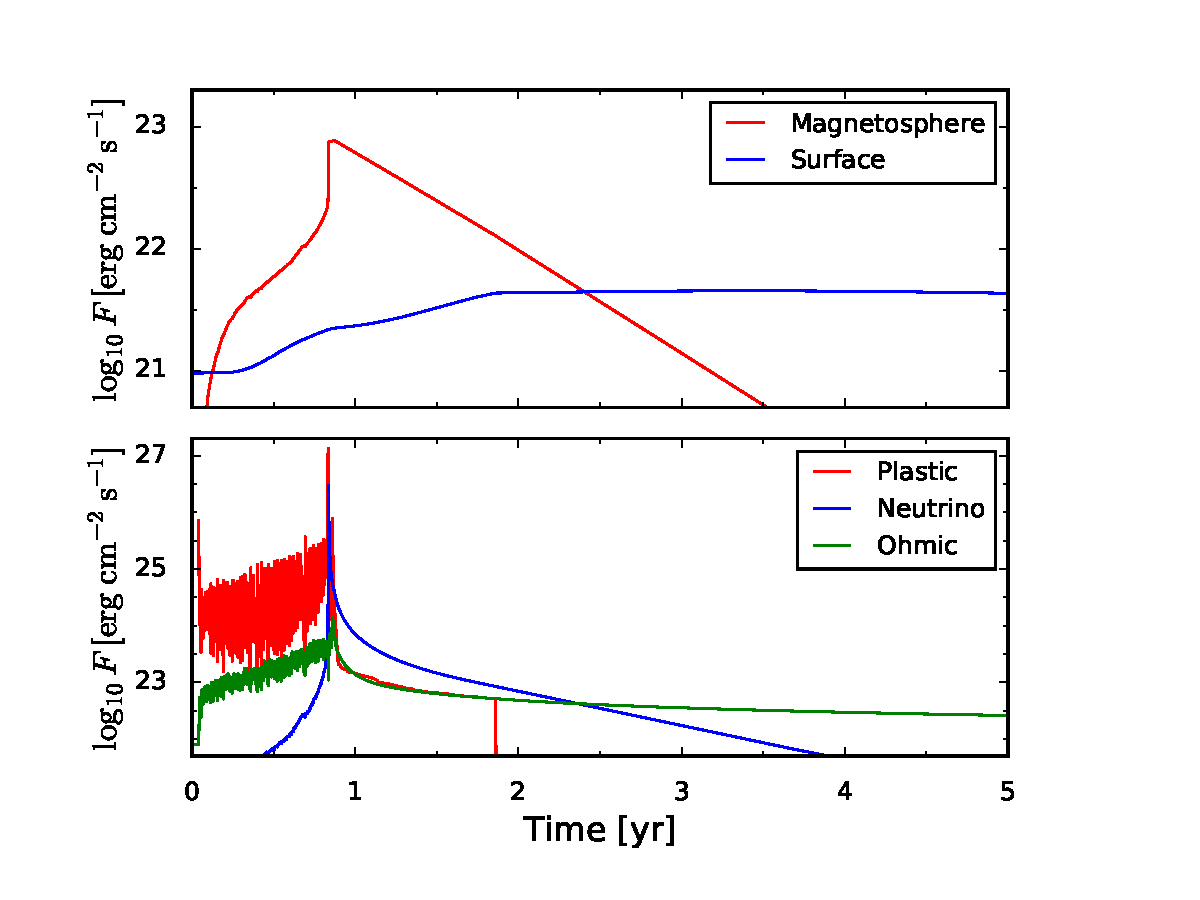
\includegraphics[width=0.6\textwidth]{pics/chap2/figz2.pdf} 
\caption[Radiation flux from the outburst simulation]{
\textbf{Upper panel:} radiation flux from the stellar surface (blue) and dissipation rate in the 
magnetosphere per unit area of the crust (red).
\textbf{Lower panel:} vertically integrated rates of plastic heating (red), ohmic heating 
(green), and neutrino cooling (blue), during and after the failure avalanche shown in 
Figure~\ref{sp2}.
}
\label{figz2}
\end{figure}
%%%%%%%%%%%%%%%%%%%%%%%%%%

The developing avalanche shears the stellar surface and pumps magnetic energy into the magnetosphere. 
This energy is gradually dissipated through the continual $e^\pm$ discharge in the magnetosphere, producing radiation that is also shown in the upper panel of Figure~\ref{figz2}.
The magnetospheric activity rises slowly  during the Hall-mediated phase, and jumps upward when the strong thermoplastic wave occurs in the end of the avalanche.
This last event is quick and suddenly implants a significant twist into the magnetosphere.
After that, the magnetospheric emission decays resistively on the timescale of a year. 
Neutrino emission also peaks during the strong thermoplastic wave, because the temperature is highest at this stage, and neutrino emission is extremely sensitive to temperature.

%%%%%%%%%%%%%%%%%%%%%%%%%%
\begin{figure*}[htbp]
\centering
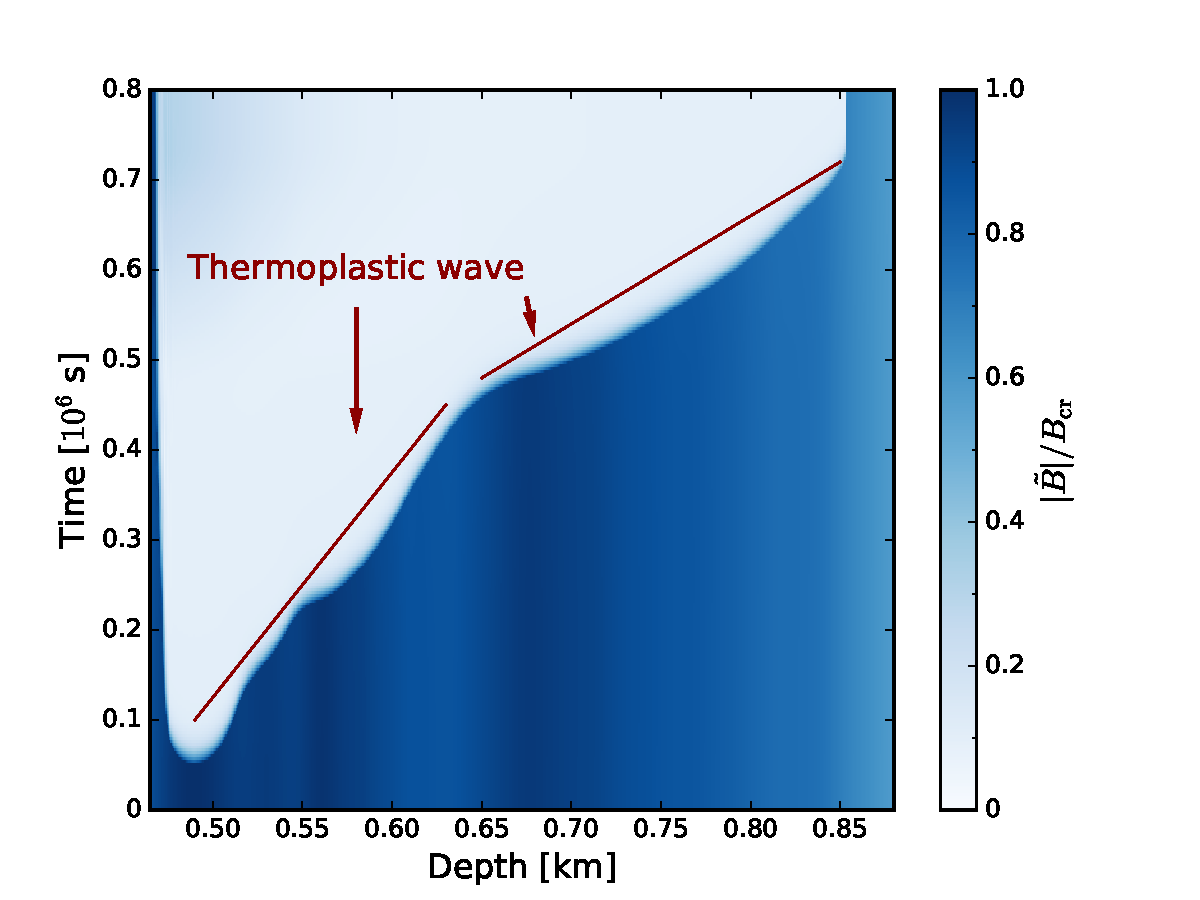
\includegraphics[width=0.48\textwidth]{pics/chap2/sp1.pdf} 
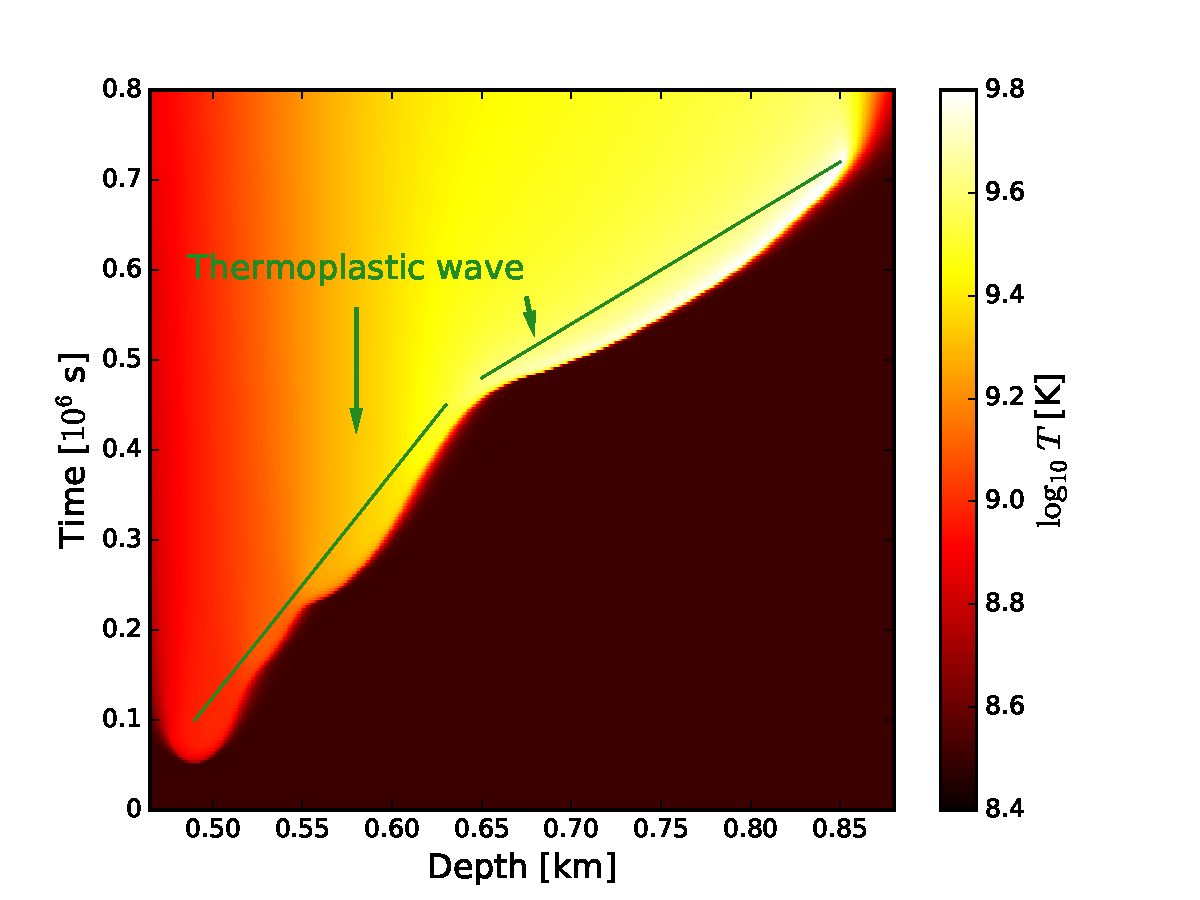
\includegraphics[width=0.48\textwidth]{pics/chap2/sp1_1.pdf} 
\caption[Spacetime diagram for a giant thermoplastic wave]{Spacetime diagram for a giant thermoplastic wave observed in the simulation at $t\approx 3.2$~kyr.
\textbf{Left panel:} evolution of $\tilde{B}/B_{\rm cr}$. 
Note the smaller scale on the time axis compared with Figure~\ref{sp2}; the thermoplastic wave is much faster than the Hall-mediated avalanche. \textbf{Right panel:} temperature evolution. 
Compared to Figure~\ref{sp2}, the heating is stronger and occurs deeper in the crust.
There is also a strong temperature gradient across the wave front. 
}
\label{sp1}
\end{figure*}
%%%%%%%%%%%%%%%%%%%%%%%%%%

%%%%%%%%%%%%%%%%%%%%%%%%%%
\begin{figure}[h]
\centering
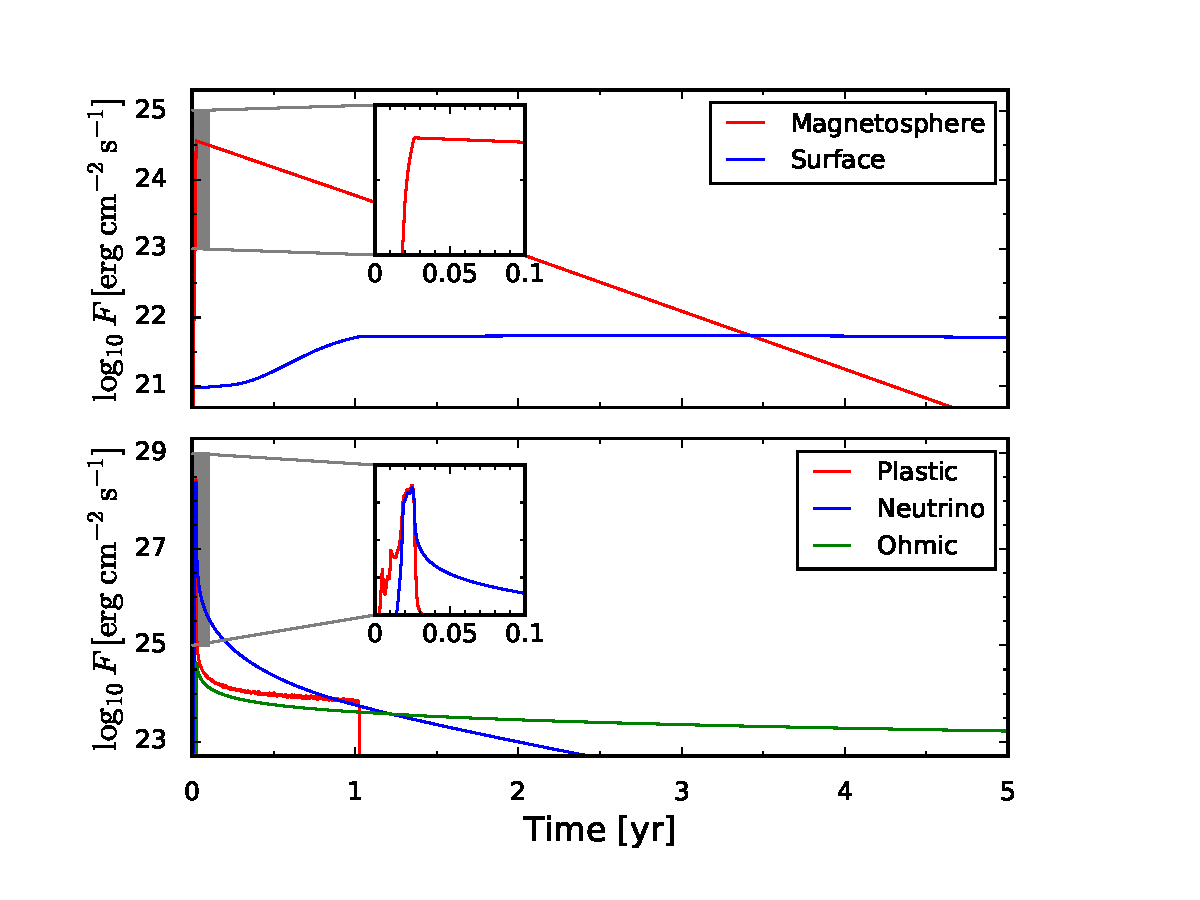
\includegraphics[width=0.6\textwidth]{pics/chap2/figz1.pdf} 
\caption[Radiation flux from the outburst simulation for a giant thermoplastic wave]{
\textbf{Upper panel:} radiation flux from the stellar surface (blue) and dissipation rate in the 
magnetosphere per unit area of the crust (red). The insets  zoom into the initial 
spike at the time of the thermoplastic wave.
\textbf{Lower panel:} vertically integrated rates of plastic heating (red), ohmic heating (green), and neutrino cooling (blue), during and after the thermoplastic wave shown in Figure~\ref{sp1}.
}
\label{figz1}
\end{figure}
%%%%%%%%%%%%%%%%%%%%%%%%%%

Figure~\ref{sp1} shows another failure at $z\sim 0.5$~km at a later time during the evolution. 
This time, $\tilde{B}$ closely approached $\Bcr$ in a broader range of depths, and the failure immediately triggers a giant thermoplastic wave, which propagates from $z\approx 0.5$~km to 0.85~km. 
It travels much faster and a longer distance compared with the Hall-mediated avalanche in Figure~\ref{sp2}. 
The temperature is higher and there is a strong temperature gradient across the wave front, which sustains its propagation.

Thermoplastic wave is a fast mode of failure propagation compared with the Hall-mediated avalanche; in this example its duration is only 0.02 year ($7\times 10^5$~s). 
It produces fast and strong heating of the crust and twisting of the external magnetosphere (Figure~\ref{figz1}). 
However, the resulting radiation flux from the stellar surface is not much higher than in Figure~\ref{figz2}.
This is because heat is deposited deeper in the crust, and a larger fraction of the heat is conducted into the core and lost to neutrinos.
This is in agreement with the behavior seen in \citet{2006MNRAS.371..477K,2014MNRAS.442.3484K}, see \citet{2016ApJ...833..261B} for a discussion of the surface heating efficiency.

%%%%%%%%%%%%%%%%%%%%%%%%%%
\begin{figure}[h]
\centering
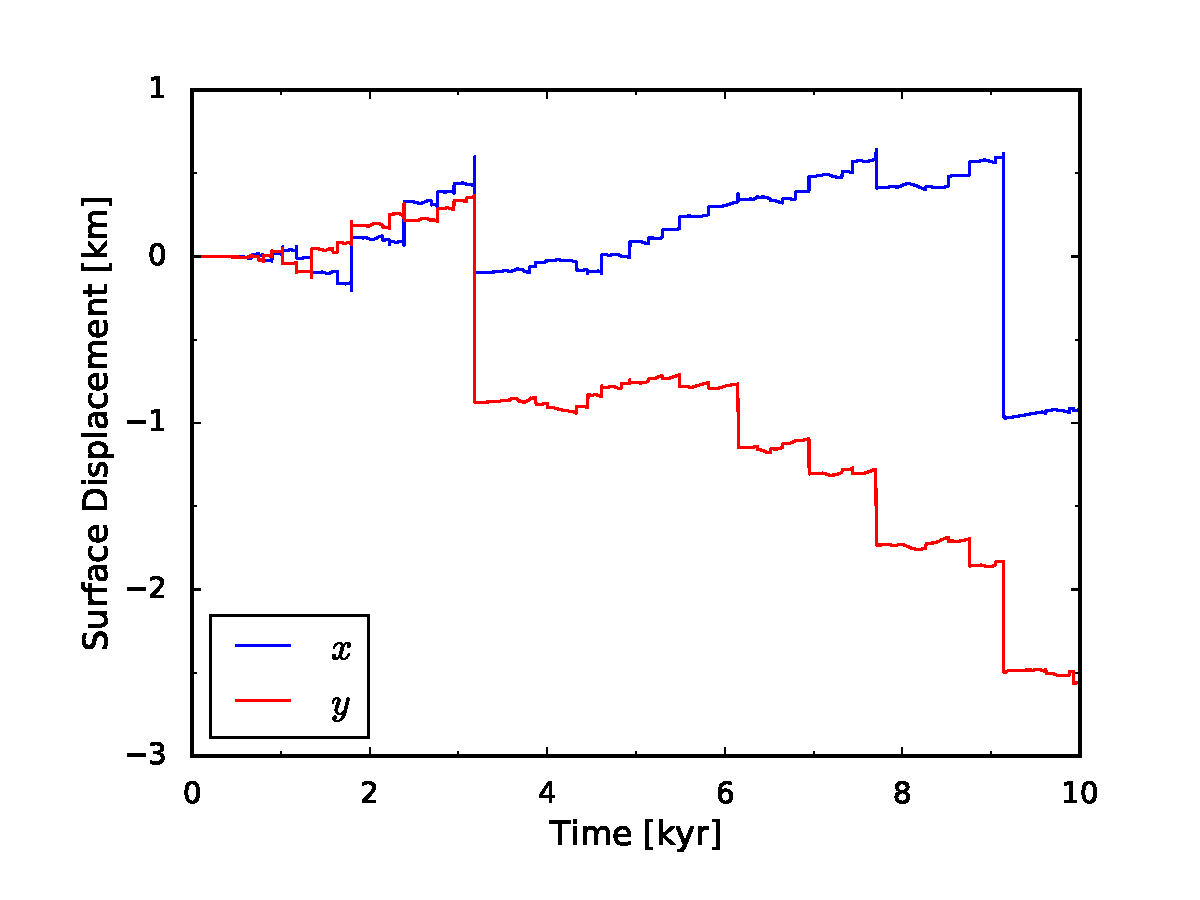
\includegraphics[width=0.6\textwidth]{pics/chap2/dis.pdf} 
\caption[Evolution of surface displacement]{Evolution of surface displacement in the horizontal $x$ and $y$ directions during the entire 10~kyr simulation.}
\label{dis}
\end{figure}
%%%%%%%%%%%%%%%%%%%%%%%%%% 

Figure~\ref{dis} shows the evolution of surface displacement in the $x$ and $y$ directions during our entire simulation. 
The displacement is zero at the beginning, before the Hall wave launched at the crust-core interface reaches the surface. 
Each failure event causes the displacement to change abruptly. The large abrupt jump in the displacement near $3$~kyr is the result of the giant thermoplastic wave shown in Figure~\ref{sp1}. 
The smaller jump near $7$~kyr corresponds to the event shown in Figure~\ref{sp2}. 
There is another large jump of $1.5$~km caused by the thermoplastic wave at $t\approx 9$~kyr.

%%%%%%%%%%%%%%%%%%%%%%%%%%
\begin{figure}[h]
\centering
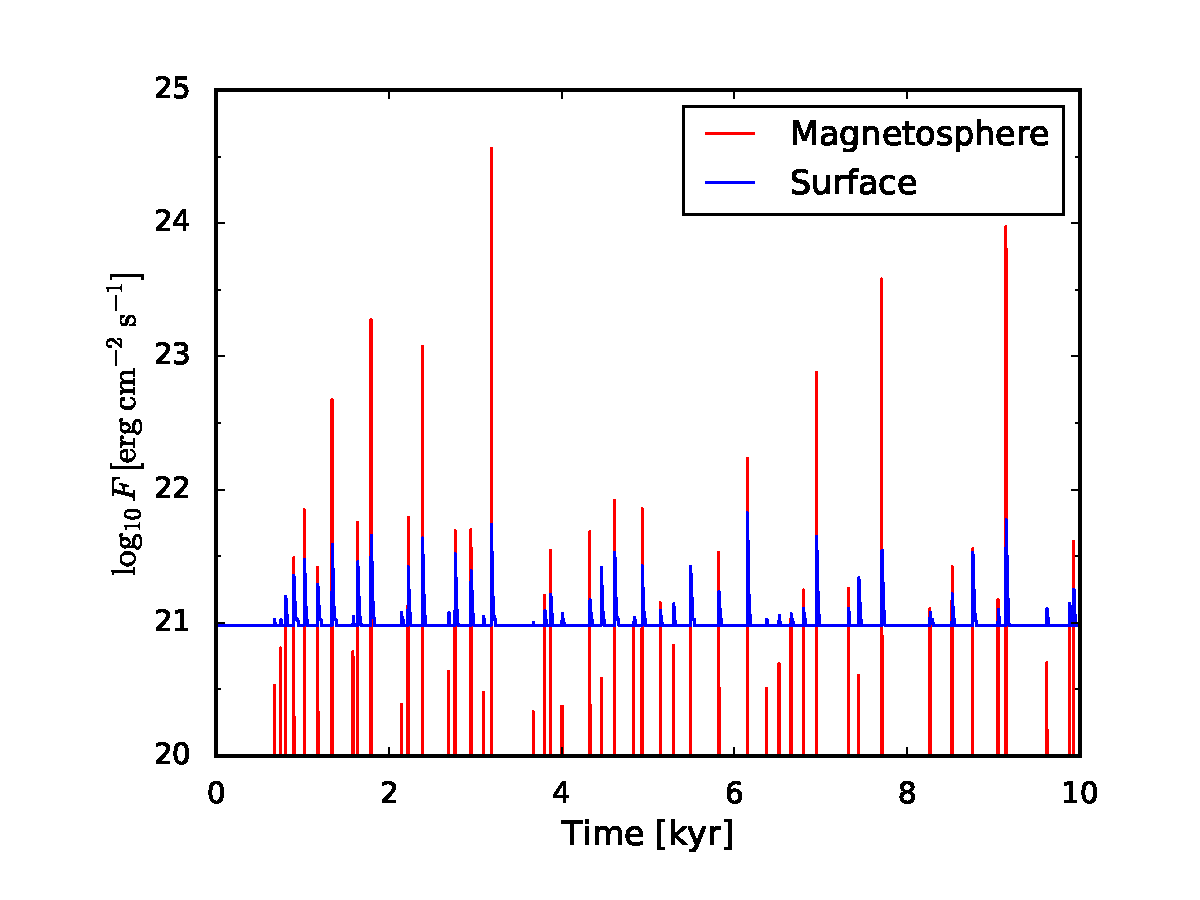
\includegraphics[width=0.6\textwidth]{pics/chap2/lum.pdf} 
\caption[Evolution of the radiation flux]{Evolution of the radiation flux from the stellar surface (blue) and dissipation rate in the magnetosphere per unit area of the crust (red) during the entire 10~kyr simulation.
}
\label{lum}
\end{figure}
%%%%%%%%%%%%%%%%%%%%%%%%%% 

Figure~\ref{lum} shows the evolution of observable radiation, from the surface and the magnetosphere, during the entire simulation. 
Both magnetospheric and surface emissions occur in sporadic spikes. 
There seems to be no obvious pattern for the spikes.
Each spike is an outburst caused by thermoplastic waves or Hall-mediated failures or a combination of both. 
The two large thermoplastic waves at $3$~kyr and $9$~kyr produce the strongest magnetospheric emission. 

%%%%%%%%%%%%%%%%%%%%%%%%%%
\begin{figure}[h]
\centering
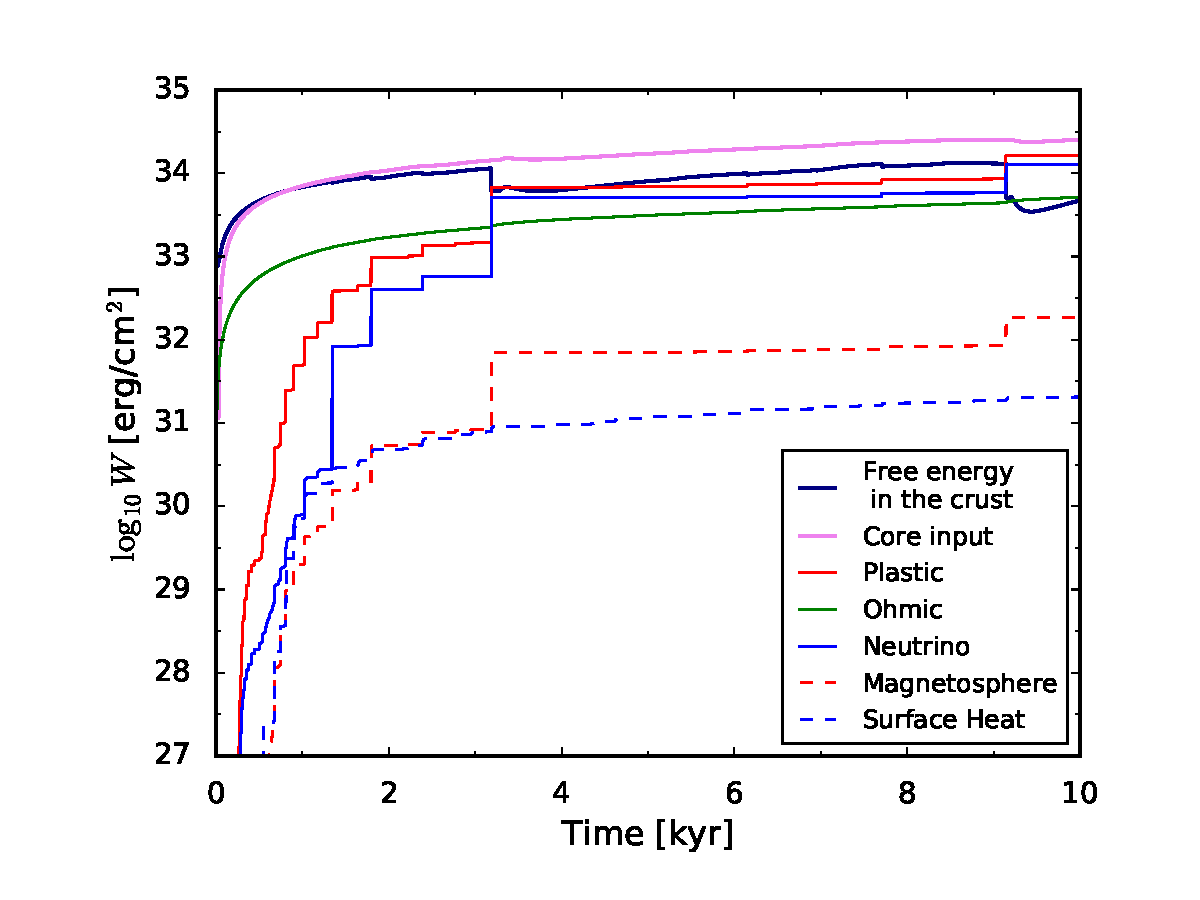
\includegraphics[width=0.8\textwidth]{pics/chap2/energy.pdf} 
\caption[Evolution of the free energy]{Evolution of the free energy stored in the crust and the contributions to its changes (see text).
}
\label{energy}
\end{figure}
%%%%%%%%%%%%%%%%%%%%%%%%%% 

Figure~\ref{energy} shows the evolution of the column density of ``free'' energy $W$ (density integrated over $z$) stored in the crust and available for dissipation; it includes the energy of the horizontal magnetic field and the elastic deformation energy. 
The figure also shows the contributions to the changes in $W$ due to the Poynting flux from the core, plastic and ohmic dissipation, neutrino losses, the Poynting flux into the magnetosphere and heat flux radiated away at the surface above the persistent background.
Whenever there is an outburst, the free energy of the crust drops while the produced (time-integrated) heat, neutrino and radiative losses rapidly increase. 
Plastic and ohmic dissipation are the two main channels by which the crust is heated, with most of the heat lost to neutrinos or conducted into the core. While the plastic heating only happens sporadically, the ohmic heating takes place continuously at a much lower  rate and has a negligible effect on the temperature change and emerging flux during the outburst. 
Only a small part of the dissipated energy (about 1\%) is injected and damped through the magnetospheric twist decay, and an even smaller part reaches the surface through heat diffusion.
It is through these two channels that the outburst produces the observable X-ray luminosity.

\section{Discussion}\label{discussion}


Hall evolution of the magnetic field provides a robust mechanism for growing 
magnetic stress in the solid crust of a magnetar, and yielding to theses stresses results in mechanical heating of the crust. 
\citet{2016ApJ...833..261B} showed that heating from internally fostered crustal failures obeys strong constraints, which prevent it from sustaining the observed high temperatures of persistently luminous magnetars. 
In agreement with these constraints, our results do not show a strong persistent heating of magnetars. 
However, the described mechanism of activity driven by Hall drift can have significant observational implications. 
The intermittent shear motions of the failed crust play a key role for twists of the external magnetosphere and also provide sporadic mechanical heating. 
This may explain outbursts of activity, in particular in the increasing number of so-called transient magnetars.

The model we have studied is one-dimensional, and therefore can only serve as a proxy for the evolution of magnetic fields and crustal deformations of real three-dimensional magnetars. 
However, we expect that the main features of the model, i.e. the avalanches of mechanical failures mediated by short wavelength Hall waves, large-scale thermoplastic waves, and the magnetospheric twists that these  cause, will be present in a more realistic three-dimensional dynamics. 
We note also that multidimensional simulations will likely show the interaction of crustal failures with the non-linear Hall dynamics that is not captured in our 1D model.
Magnetic instabilities in 2D or 3D, e.g. density-shear instability  \citep{2014PhPl...21e2110W,2015MNRAS.453L..93G}, will provide other channels to launch Hall waves by creating current sheets in the crust \citep{2016PNAS..113.3944G}.
In what follows we comment on how the simulated outbursts in our model compare with the observed outbursts.

During an outburst of a transient magnetar the observed X-ray flux increases by a factor of 10-1000 compared to its quiescent level and typically decays on the time scale of months to years. A canonical example is provided by the first discovered  transient magnetar  XTE J1810-197 \citep{2004ApJ...609L..21I}, with the characteristic dipole magnetic field $\sim 3\times 10^{14}$~G. 
It was discovered in January 2003 when its X-ray luminosity was comparable to $10^{35}$~erg~s$^{-1}$, which is a factor of $\sim 100$ above the quiescent level. 
It returned back to the quiescent level in a few years \citep{2007Ap&SS.308...79G}.
However, no data is available for the early phase of this event (from Nov. 2002 to Jan. 2003) and so one cannot observationally study the rise of its light curve. 
The spectral fits of the outburst showed the appearance and subsequent shrinking of a hot spot on the star of size $\lesssim 3$~km, which indicates a localized twist of the external magnetosphere. 
The transient magnetar discovered recently in the Galactic Centre SGR~1745$-$2900 \citep{2013ApJ...770L..24K,2013ApJ...770L..23M} is almost a twin of  XTE~J1810-197. Its outburst showed a similar decay, with a similar shrinking hot spot \citep{2014ApJ...786...84K,2015MNRAS.449.2685C}.
Similar strong outbursts were observed in several other transient magnetars (see \citet{2011ASSP...21..247R} for a review).

Less dramatic outbursts are also observed in ``persistent'' magnetars that show a continuously high level of emission during decades of observations. 
For instance, the long-term observations of 1E 1048.1-5937 captured four outbursts (and resolved their rise times) between 2001 and 2007 \citep{2008ApJ...677..503T}. The 2001-2002 event increased the X-ray luminosity by a factor of $\sim 2$ over $\sim 20$ days and then decayed over
$\sim$100 days \citep{2004ApJ...609L..67G}. 
The rise times of the 2002 and 2004 outbursts were a few weeks. 
The 2007 outburst rose to its peak in less than a week \citep{2008ApJ...677..503T}.

How does this data stack up against our model?  
The model predicts spikes in surface radiation flux of $10^{22}-10^{24}$~erg~s$^{-1}$~cm$^{-2}$. 
Assuming an emission area of about $10^{11}\hbox{cm}^2$ ($3\hbox{~km}\times 3\hbox{~km}$), our simulated peaks of luminosity are $10^{33}-10^{35}$~erg/s. 
The typical decay time of luminosity after the end of the failure event is typically comparable to one year. These values are in good agreement with observations.

In our model, we have three different timescales: the timescale of thermoplastic waves (controlled by parameter $\alpha$), Hall-mediated avalanches, and heat diffusion. 
The heat diffusion timescale is  comparable to one year and independent of the plastic-flow constant $\alpha$. 
It controls both the rise and the decay of surface luminosity due to heat diffusion from the heated interior to the surface. 
The observed rise times in the sources described above are often much shorter, more consistent with the timescale of magnetospheric twisting by thermoplastic waves. 
This suggests that the onset of the outburst is controlled by magnetospheric dissipation induced by the plastic motions of the crust. 
These motions extract energy from the stellar interior (through Poynting flux) much faster than heat diffusion, and with a higher efficiency. 
A significant fraction of energy dissipated in the magnetosphere should be delivered to the surface by accelerated particles and radiated from the surface. 
There is strong observational evidence for this external heating of the magnetar surface, see \citet{2016ApJ...833..261B}.

Our simulation shows that the outburst rise time depends on whether the crustal failure develops through a Hall-mediated avalanche or a large-scale thermoplastic wave.
The rate of crustal failure (and the corresponding surface shear rate) in both cases is proportional to $\alpha^{1/2}$, see \Eqs~(\ref{eq:vTPW}) and (\ref{eq:vH}), and their ratio is independent of $\alpha$. 
The Hall-mediated avalanche is slower by the factor of $(D_{\rm H}/\chi)^{1/2}$, where $D_{\rm H}=(cB_z/4\pi en_e)$ is the Hall diffusion coefficient and $\chi=\kappa/C_V\sim 10-100$~cm$^2$~s$^{-1}$ is the heat diffusion coefficient.
The factor $(D_{\rm H}/\chi)^{1/2}$ is typically around $10^{-2}$. The value of $\alpha$ is unknown, and both failure modes can be fast, giving short outburst rise times.
For the choice of parameters in our simulations, $\alpha=10^{-4}$~s$^{-1}$, the typical outburst light-curve from a  thermoplastic wave rises to its peak in days to weeks.
The decay occurs on the much longer timescales of resistive magnetospheric untwisting and heat diffusion through the crust. Both of these timescales are known to be roughly comparable to one year.

In our simulation, we see a large outburst every several hundred years. 
However, our simple 1D model simulates only a small patch on the magnetar surface --- our simulation box may represent a crustal plate with surface area of a few square kilometers (as the crust thickness is about one kilometer). 
There may be hundreds of such independent patches, each undergoing its own series of outbursts. 
2D or 3D simulations will be required to model the global picture, which can give much more frequent outbursts. 
The outburst rate also increases with increasing $B_{\rm core}$.
Our simulations assumed $B_{\rm core}=6\times 10^{15}$~G, and a higher value would increase the magnetic energy flux from the core into the crust and make it easier to initiate plastic failures in the deeper crust.

In this chapter we concentrated on the relatively slow dynamics of outbursts. 
Therefore our results do not directly apply to the distinct class of magnetar bursts and flares that have much shorter durations, with rise times much shorter than one second. 
\citet{1995MNRAS.275..255T,1996ApJ...473..322T} proposed that the bursts result from sudden ``brittle" failures in the crust. 
It is, however, unclear how the compressed magnetized material with pressure well above the Coulomb lattice energy could be brittle \citep{2003ApJ...595..342J,2012MNRAS.427.1574L,2014ApJ...794L..24B}.
Therefore, it appears more likely that the fast flares result from explosive relaxation of the twisted magnetosphere \citep{1995MNRAS.275..255T,2006MNRAS.367.1594L,2012ApJ...754L..12P,2013ApJ...774...92P}. 
These magnetospheric explosions also produce sudden deformations of the crust 
\citep{2015ApJ...815...25L} which leave strong gradients in the crustal magnetic field and may be followed by accelerated Hall evolution. Both ``internal'' (brittle) and ``external'' (magnetospheric) models could be related to the clusters of ``storm bursts''  \citep{2006A&A...445..313G,2008ApJ...685.1114I,2010MNRAS.408.1387I,2011ApJ...739...94S} if the Hall evolution induced by a burst leads to more bursts.

The avalanches of thermoplastic failures and heating of the crust may affect the rotation rate of the magnetar by changing the rotation of the neutron superfluid in the lower crust. 
The superfluid vortices could become unpinned from the crustal lattice, resulting in timing anomalies --- glitches or anti-glitches associated with outbursts.
We defer the study of this possibility to future work.

% Local Variables:
% TeX-master: "../thesis"
% zotero-collection: #("16" 0 2 (name "Thesis"))
% End:

\zotelo{../thesis.bib}

\def\T{{\mathcal T}}
\def\scr{s_{\rm cr}}
\def\Ts{T_{\rm s}}
\def\Tm{T_{\rm melt}}
\def\zmelt{z_{\rm melt}}
\def\beq{\begin{equation}}
\def\eeq{\end{equation}}
\def\sel{s_{\rm el}}
\def\spl{s_{\rm pl}}
\def\dspl{\dot{s}_{\rm pl}}
\def\sigcr{\sigma_{\rm cr}}
\def\Um{U_{\rm melt}}
\def\Uth{U_{\rm th}}
\def\Eq{Equation}
\def\Eqs{Equations}
\def\Ekin{E_{\rm kin}}
\def\Emag{E_{\rm mag}}
\def\Eel{E_{\rm el}}
\def\zd{z_{\rm damp}}
\def\Eaft{E_{\rm aft}}
\def\tc{t_{\rm cond}}
\def\LL{L}
\def\lw{l}
\def\Lum{\mathcal{L}}

\chapter[Plastic Damping  of Alfv\'en Waves in Magnetar Crusts]{Plastic Damping  of Alfv\'en Waves in Magnetar Crusts}
\label{chap:plastic-damping}
 \alfven waves are generated with a total energy up to $\sim 10^{46}$~erg during the giant flares. 
They are trapped on the closed magnetic field lines, as the group velocity of \alfven waves is parallel to the magnetic field. The fate of their energy is poorly known. 
It was proposed that the \alfven waves can be damped through nonlinear processes 
\citep{1998PhRvD..57.3219T}, which become efficient at very large amplitudes of the waves.

In this chapter, we propose another  mechanism of the \alfven wave dissipation, which 
results from the wave interaction with the star. 
The waves are ducted along the magnetic field lines with nearly speed of light and reach the stellar surface on a millisecond timescale. 
We examine the wave interaction with the star and find that a significant fraction of the wave energy is transmitted into the stellar crust. 
The reflected waves keep bouncing in the magnetosphere, however in a few tens of milliseconds most of their energy is drained and deposited into the crust, in the form of a compressed shear wave packet. 
We show that this packet causes strong plastic heating of the crust. 
We investigate the fate of heat deposited by the plastic damping of \alfven waves. 
In particular, we evaluate the heat flux conducted back to the surface and the resulting surface luminosity, which should emerge long after the flare. 

\section{Wave transmission into the crust}\ref{wave-dyn}

The crust is nearly incompressible and supports shear waves which can be excited by the \alfven waves impinging from the magnetosphere. 
Excitation of two-fluid crustal modes can be neglected, and the recent claim that magnetospheric \alfven waves  transform into crustal Hall waves \citep{2015MNRAS.447.1407L} is incorrect.
Hall waves propagating parallel to the magnetic field ${\mathbf B}$ with frequency $\omega$ in the crust of density $\rho$ have refraction index 
${\cal N}=ck/\omega=\omega_{\mathrm{pe}}/\sqrt{\omega\omega_B}
\approx 10^{9}\, \rho_{11}^{1/2} \omega_5^{-1/2} B_{14}^{-1/2}$. 
%(we use the standard notation $X_m=X/10^m$ for a quantity $X$ in cgs units). 
This implies a huge impedance mismatch with the magnetospheric \alfven waves, which have ${\cal N}\approx 1$, and therefore their transformation to Hall waves is suppressed.
\footnote{Only electrons move in a Hall wave (analogous to whistler in plasma physics) while ions are static.
The velocity of the electron fluid $\mathbf{v}_H=\mathbf{j}/en_e$ is related to electric current $\mathbf{j}=(c/4\pi)\nabla\times {\mathbf B}$, which gives a tiny $v_{\rm H}$ because of the high electron density $n_e$ in the crust. 
Therefore, the ``two-fluid"(electron-ion) description is useful only for slow phenomena in the crust.}
No significant separation between electron and ion velocities can occur on ms timescales, and the response of the crust to the external disturbance is essentially single-fluid.
     
\subsection{Transmission coefficient}

Consider a magnetospheric \alfven wave of frequency $\omega$ impinging on the crust of the neutron star. For simplicity let us assume that the initial (unperturbed) magnetic field $B_z$ is uniform and vertical, so the wave is propagating vertically along the $z$-axis, and the horizontal displacement $\xi(z)$ is along the $y$-axis. 
The plasma-filled magnetosphere and the crust are excellent conductors; therefore the magnetic field is frozen in the medium and the horizontal field $B_y$ is related to the displacement by $B_y/B_z=\partial\xi/\partial z$.
The wave speed in the magnetosphere is close to the speed of light $c$, and the wavelength is $\lambda_0=2\pi c/\omega$. 

The wave propagation is described by the equation,
\begin{equation}
\label{eq:wave}
   \left[\rho(z)+\frac{B_z^2}{4\pi c^2}\right]\frac{\partial^2\xi}{\partial t^2} 
   = \frac{B_z^2}{4\pi}\frac{\partial^2\xi}{\partial z^2} - \frac{\partial\sigma}{\partial z}. 
\end{equation}
Here $\rho(z)$ is the mass density and $\rho+B_z^2/4\pi c^2$ can be thought of as the effective inertial mass density of the magnetized medium.
\footnote{This expression is approximate as it neglects the contribution from the horizontal field component $B_y$. 
In the models presented below, $B_y>B_z$ when the wave propagates into the crust; however, this only occurs in the dense region where $B^2/4\pi\ll \rho c^2$ and the magnetic field inertia anyway may be neglected. 
In the region where $B^2/4\pi\gg \rho c^2$ the wave amplitude $s=B_y/B_z<1$ and it is acceptable to approximate $B^2\approx B_z^2$.}
The first term on the right-hand-side describes the restoring force of magnetic tension, and the last term describes the force due to the shear stress in the medium.

%%%%%%%%%%%%%%%%%%%%%%%%%%
\begin{figure}[h]
\centering
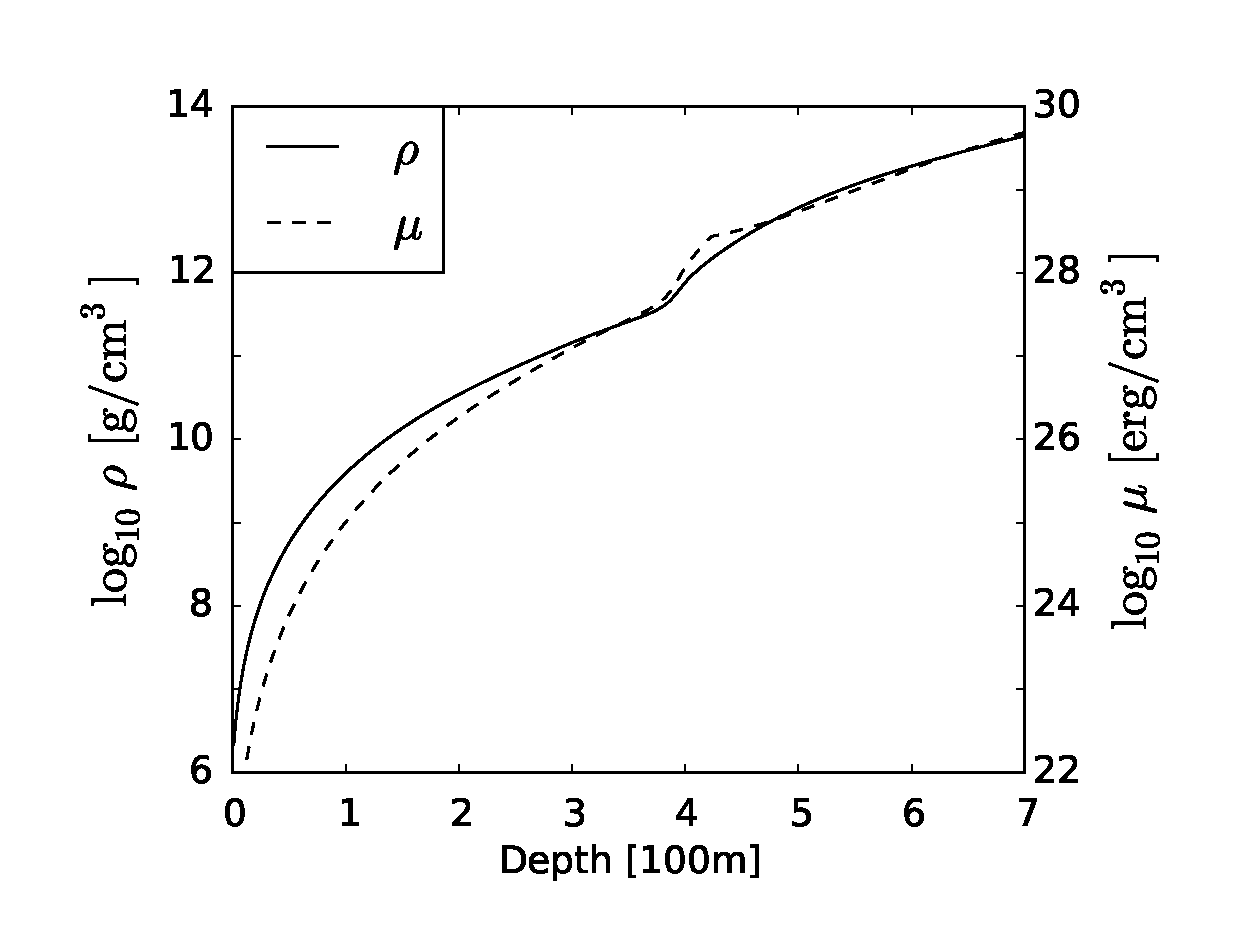
\includegraphics[width=0.6\textwidth]{pics/chap3/fig1.eps} 
\caption[Density $\rho(z)$ and shear modulus $\mu(z)$ of the neutron star crust]{Density $\rho(z)$ and shear modulus $\mu(z)$ of the neutron star crust. 
The star is assumed to have mass $M=1.4 M_{\odot}$ and SLy equation of state.}
\label{fig1}
\end{figure}
%%%%%%%%%%%%%%%%%%%%%%%%%%

In particular, if the medium is elastic with a shear modulus $\mu$ then $\sigma = -\mu s$, where $s=\partial\xi/\partial z$ is the strain of the elastic deformation. 
In this case, Equation~(\ref{eq:wave}) becomes a simple wave equation with the wave speed given by
\begin{equation}
  v^2(z)=\frac{B^2_z/4\pi+\mu(z)}{B^2_z/4\pi c^2+\rho(z)}. 
\end{equation}
In the magnetosphere, we will neglect the mass density $\rho$ and the shear modulus $\mu$, which gives $v=c$. In the crust, we will use the profiles $\rho(z)$ and $\mu(z)$ shown in Figure~\ref{fig1}. 
The density profile is obtained from the relativistic hydrostatic equation using SLy equation of state \citep{2004A&A...428..191H} for a neutron star with mass $M=1.4M_{\odot}$.
\footnote{The ultrastrong magnetic field significantly changes pressure where the electron Fermi energy is below the Landau energy. 
This impacts the density profile $\rho(z)$ at shallow depths. However, at depths of interest in this chapter (where $\rho\gg 10^8$~g~cm$^{-3}$) this effect is small and neglected.}     
The radius of the star is $R=11.7\rm ~km$, and its surface gravitational acceleration is $g = (GM/R^2)(1-r_g/R)^{-1/2}=1.7\times 10^{14}$\, cm~s$^{-2}$ where $r_g=2GM/c^2$.
For the shear modulus $\mu$ we use the fitting formula given by \citet{2005ApJ...634L.153P} and \citet{2007MNRAS.375..261S} for low and high densities. 

As the wave propagates into the deeper crust, its speed is reduced and its wavelength is compressed,
\begin{equation}
   \lambda(z) = \lambda_0 \frac{v(z)}{c},  \qquad \lambda_0=\frac{2\pi c}{\omega}.
\end{equation}

The reflection of the wave occurs in the region where the characteristic scale-height for the change of $v(z)$,
\begin{equation}
   h(z)=\frac{v}{|dv/dz|},
\end{equation} is smaller than the wavelength $\lambda(z)$. Figure~\ref{fig2} shows $\lambda(z)$, $h(z)$, and the depth $z_1$ where they are equal. 
The typical value of $z_1$ is around 200 meters below the surface; its exact value depends on $B_z$.

%%%%%%%%%%%%%%%%%%%%%%
\begin{figure}[h]
\centering
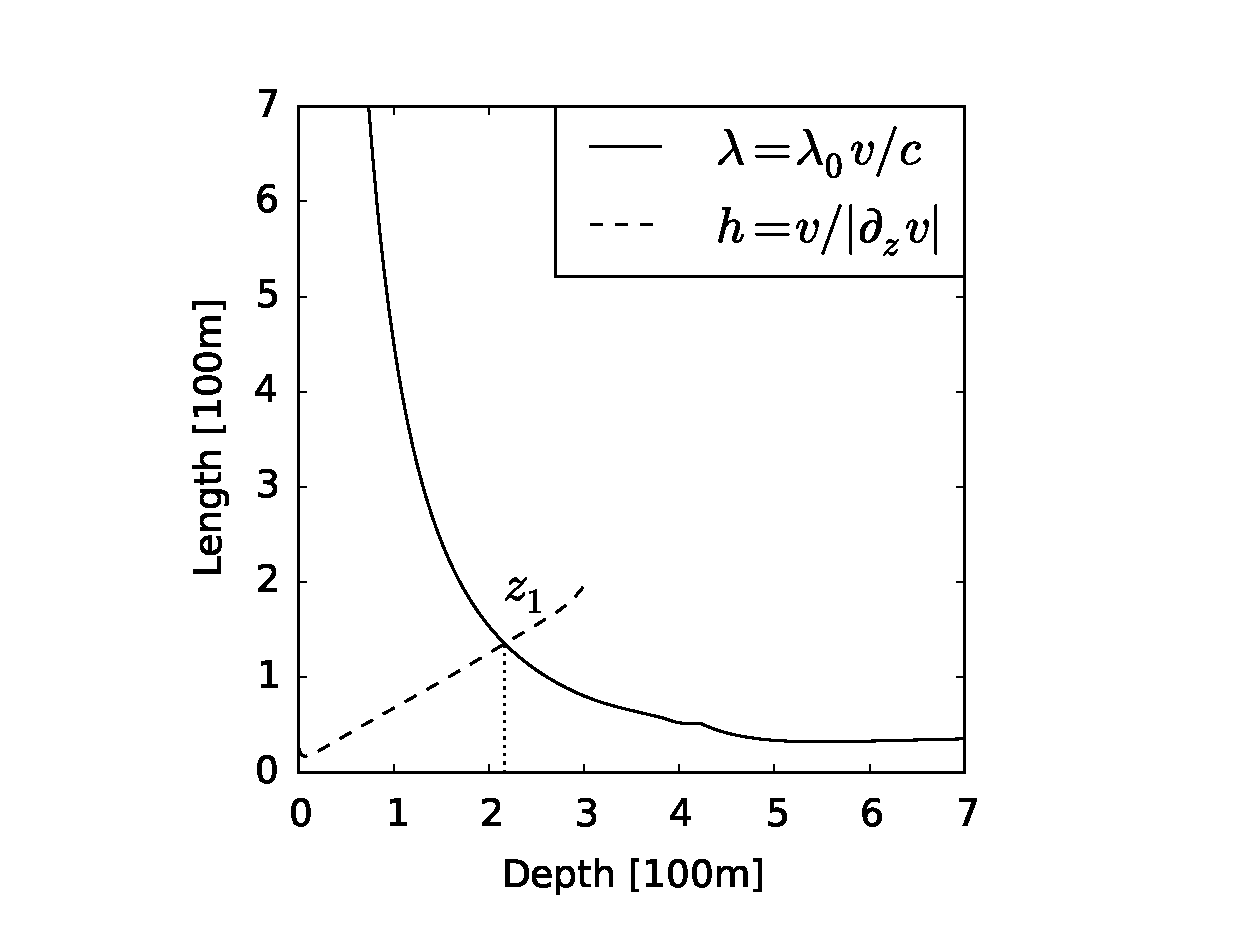
\includegraphics[width=0.6\textwidth]{pics/chap3/fig2.eps} 
\caption[Comparison between wavelength and characteristic scale in the crust]{Solid curve shows the wavelength of the shear wave propagating in the 
magnetized crust, $\lambda = \lambda_0 v/c$, where $\lambda_0=10\,\rm km$ and 
$v$ is the speed of the wave. Dashed curve shows the characteristic scale-height of 
the wave deceleration, $h= v/|\partial_z v|$. A vertical magnetic field 
$B_z = 3\times 10^{14}\,\rm G$ is assumed in this example.}
\label{fig2}
\end{figure}
%%%%%%%%%%%%%%%%%%%%%%

The transmitted wave below $z_1$ has $\lambda\ll h$ and can be described in the WKB approximation. 
Then the wave displacement takes the form (e.g. \citet{f13}),
\begin{equation}
\label{eq:xi}
  \xi(z) = \frac{\rm const}{Z^{1/2}(z)}\cos\left[\omega\left( t-\int_0 ^z \frac{\md z'}{v(z')}\right)\right],
\end{equation}
where $Z(z)$ is the impedance,
\begin{equation}
\label{eq:Z}
  Z(z)=\left[\frac{B_z ^2}{4\pi}+\mu(z)\right]^{1/2}
          \left[\frac{B_z^2}{4\pi c^2}+\rho(z)\right]^{1/2}.
\end{equation}

A simple estimate for the transmission coefficient is obtained using the impedance at $z_1$ \citep{1989ApJ...343..839B},
\begin{equation}
\label{eq:TC}
   \mathcal{T}\sim \frac{4Z(z_1)Z(0)}{\left[Z(z_1)+Z(0)\right]^2} 
   \approx \frac{4v(z_1)}{c}. 
\end{equation}
For instance, for $B_z=3\times 10^{14}\,\rm G$, Equation~(\ref{eq:TC}) gives 
$\mathcal{T}\sim 5\%$. 
A more accurate transmission coefficient is obtained by solving numerically the wave equation, which gives a higher value of $\T=12$\% (the smoothness of the crustal density variation as the wave approaches $z_1$ 
enhances the transmission). 
The numerically calculated $\T(B_z)$ is shown in Figure~\ref{fig3}. It is comparable to 0.1 for typical magnetar fields.
%%%%%%%%%%%%%%%%%%%%%%
\begin{figure}[h]
\centering
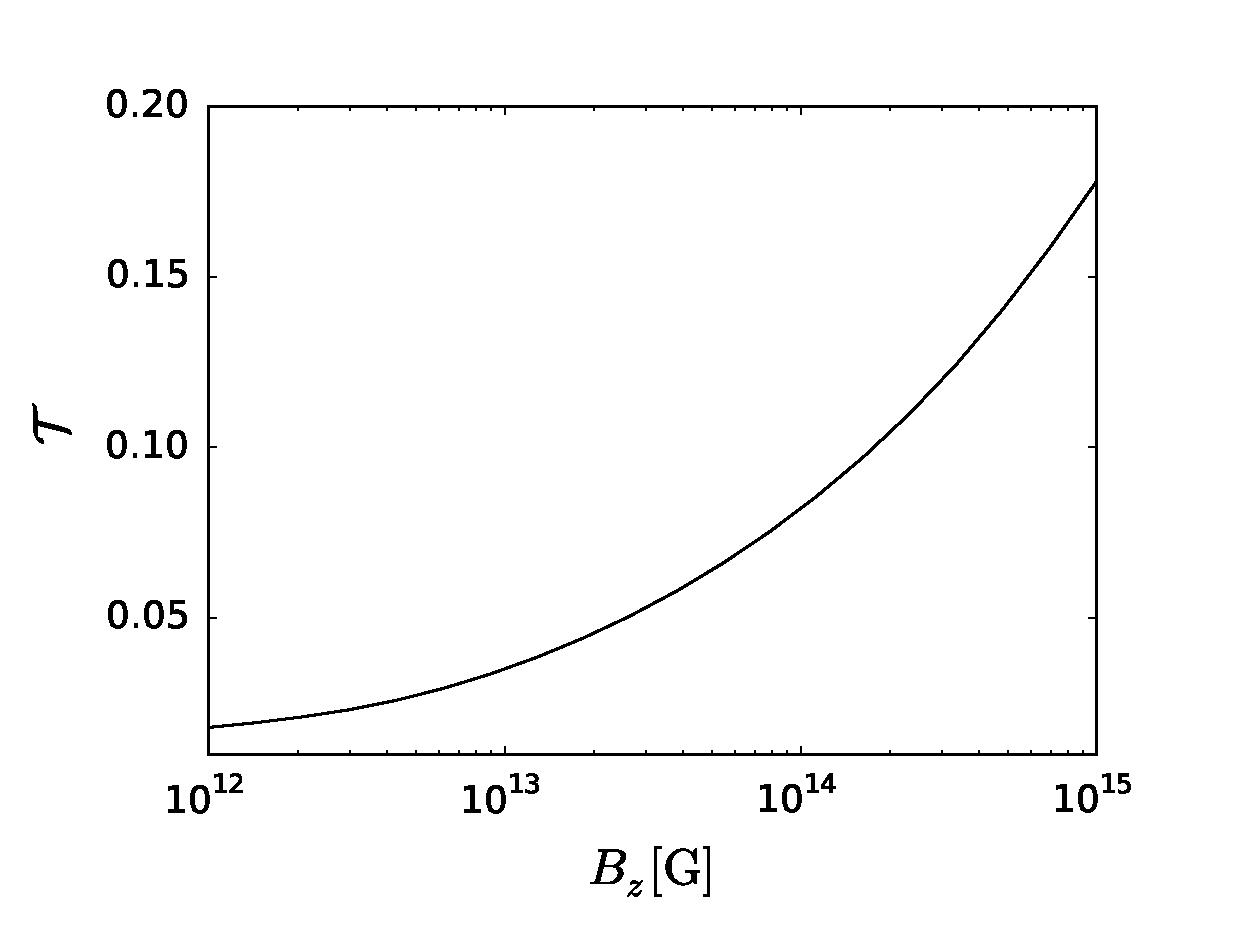
\includegraphics[width=0.6\textwidth]{pics/chap3/fig3.eps} 
\caption[Transmission coefficient $\mathcal{T}$ as a function of vertical magnetic 
field $B_z$]{Transmission coefficient $\mathcal{T}$ as a function of vertical magnetic 
field $B_z$, obtained from the numerical solutions of Equation~(\ref{eq:wave}).}
\label{fig3}
\end{figure}
%%%%%%%%%%%%%%%%%%%%%%

The reflection coefficient ${\mathcal R}=1-\T\sim 0.9$ is large, and the reflected Alfv\'en waves will bounce many times in the magnetosphere. Their amplitudes decrease by $\T\sim 10$\% every time they bounce from the surface. 
The repeated transmission events form a train of compressed waves in the crust. 
This train propagates into the crust with velocity $v\sim 10^{-2}c$.

One can show from Equation~(\ref{eq:xi}) that the strain $s=\partial\xi/\partial z$ in the transmitted wave evolves as $|s|\propto v^{-1}Z^{-1/2}\propto\rho^{1/4}$. It {\it increases} as the wave propagates into the deeper and denser crust. 
This has a simple physical reason: the wave decelerates, and hence its energy density $U_w$ grows as $v^{-1}$ 
(so that the wave continues to carry its energy flux $F_w=U_w v=const$). 
The wave energy oscillates between the kinetic energy and the horizontal field plus elastic energy of the crust. 
Therefore, $U_w$ may be written in two ways: $U_w\sim (\rho+B^2/4\pi c^2)\, \xi^2 \omega^2$ (kinetic) or $U_w\sim s^2 (B_z^2/4\pi+\mu)$ (magnetic+elastic). 
In the region where $\rho c^2>B^2/4\pi$ and $\mu<B_z^2/4\pi$ this requires $\xi^2\propto (\rho v)^{-1}$ and $s^2\propto v^{-1}$. 
Then the relation $s\sim \xi/\lambda\propto \xi/v$ gives 
\beq
 \xi\propto v^{1/2}, \qquad v\propto \rho^{-1/2}, \qquad  s\propto \rho^{1/4}.
\eeq 
In the lower crust where $\mu\gtrsim B_z^2/4\pi$ and $v\approx(\mu/\rho)^{1/2}\approx const \approx 10^8$~cm~s$^{-1}$ one finds $s\propto\rho^{-1/2}$. 
In this region the wave strain significantly decreases. 
This evolution of $s$ with depth (increase and then decrease) may be observed in the numerical simulation presented below.

\subsection{Numerical model}\label{sec:numerical}

To illustrate the transmission process we set up a simple one-dimensional simulation of waves bouncing in the magnetosphere between the footprints of a closed magnetic flux tube.
The \alfven waves are ducted along the magnetic field lines and the problem can be made one-dimensional by pretending that the flux tube is straight, and by placing its two opposite footprints on the $z$-axis, separated by distance $\LL$.
Here $\LL$ represents the length of magnetospheric field lines.
The stellar crust with the density profile $\rho(z)$ is placed symmetrically at the two ends of the computational box. 
The crust thickness $\sim 1$~km is much smaller than $\LL$.

For any initial shear distortion of the field lines, one can calculate the subsequent 
dynamics of the generated \alfven waves by solving numerically Equation~(\ref{eq:wave}). 
In our numerical models, we take the initial distortion of the form, 
\begin{equation}
    \xi_0(z) = A \exp\left[-\frac{(z-z_0)^2}{2\lw^2}\right],
\end{equation}
which is localized in the middle of the box $z_0$, far away from the crust, with 
$\lw< \LL$.
The distortion immediately splits into two waves propagating toward the opposite ends of the box. 
The strain profile of each wave $s(z)=\partial\xi/\partial z$ is determined by the initial distortion. 
An important parameter of the wave is its initial maximum strain,
\beq
   s_0=\frac{1}{2}\,\max |\partial_z \xi_0(z)|=\frac{A}{2\lw}\,e^{-1/2}.
\eeq
The total energy initially stored in the two waves is
\begin{equation}
    E_{0}=\frac{\sqrt{\pi}}{8\pi}\,B_z^2\,\frac{A^2S}{\lw},
\end{equation}
where $S$ is the cross section area of the flux tube.

%%%%%%%%%%%%%%%%%%%%%%
\begin{figure}[h]
\centering
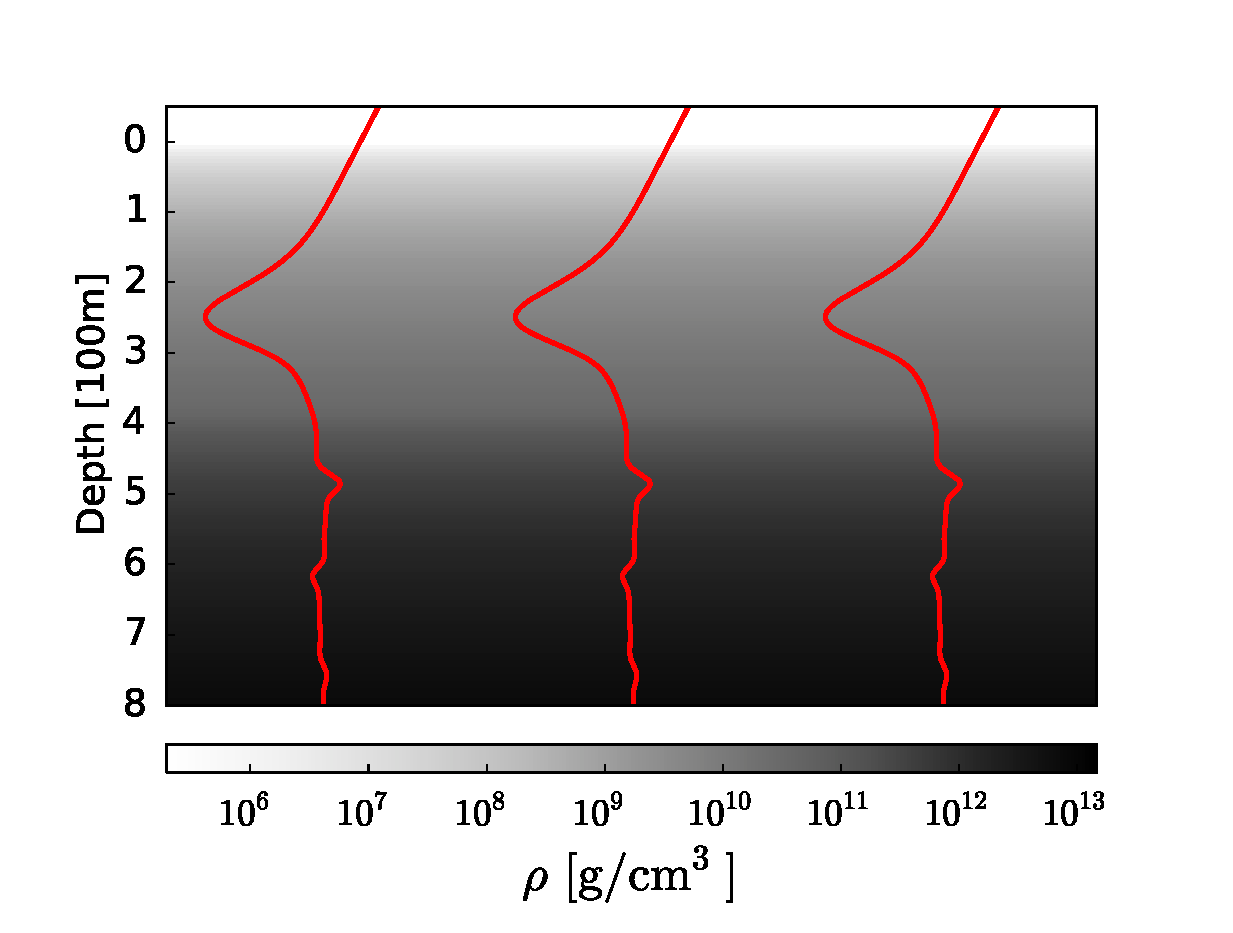
\includegraphics[width=0.6\textwidth]{pics/chap3/fig4.eps} 
\caption[A snapshot of the wave after four reflection/transmission events]{A snapshot of the wave after four reflection/transmission events. 
Solid red curves show the magnetic field lines deformed by the horizontal displacements in the wave; background grey color shows the density of the crust. 
The wave front has reached the depth of 800~m by this time. 
One can see the four oscillations in the transmitted and compressed packet. 
The shape of each oscillation reflects the initial shape of the magnetospheric wave assumed in the simulation.
This simulation included no plastic dissipation and assumed the magnetic field $B_z = 3\times 10^{14}\,\rm G$.}
\label{fig4}
\end{figure}
%%%%%%%%%%%%%%%%%%%%%%

We follow the evolution of the waves and their interaction with the crust until almost all wave energy $E_0$ has been drained from the magnetosphere; this typically takes tens of light-crossing times $\LL/c$. 
The wave equation~(\ref{eq:wave}) is solved on a grid with 1000 points in the magnetosphere (uniformly spaced) and a much finer grid in the crust (one point per meter). 
Convergence tests have been done to ensure that the grid is sufficiently large to resolve the wave dynamics.

The snapshot of the simulation in Figure~\ref{fig4} shows the distortion of the crust at time $t=4.6\LL/c$, when the magnetospheric waves have bounced four times. 
The parameters of this sample model are $\LL=40$~km, $\lw=5/\sqrt{2}$~km, $A=5$~km, and $B_z=3\times 10^{14}$~G. 
The corresponding $s_0=(2e)^{-1/2}\approx 0.43$ and $E_0/S\approx 4.5\times 10^{32}$~erg~cm$^{-2}$.
In the snapshot shown in the figure, about 1/3 of the wave energy $E_0$ has already been transmitted into the crust. 
The transmitted wave has been decelerated to $v\approx 10^8$~cm~s$^{-1}$ and compressed by the factor of $c/v\approx 3\times 10^2$. 
The compression creates a high energy density of the horizontal magnetic field at $z=200-500$~m, $(sB_z)^2/8\pi\sim 10 (s_0B_z)^2/8\pi$, and strain $s\sim 3s_0$.

\section{Plastic Heating}

The description of the wave dynamics in Section~\ref{wave-dyn} is incomplete because it assumes the elastic response $\sigma=-\mu s$ everywhere in the crust.
The more realistic model must take into account two facts:
(1) When the solid crust is deformed by the shear wave beyond a critical stress 
$\sigcr$ its response becomes plastic rather than elastic.
(2) The crustal temperature may be high enough to reduce $\sigcr$ or even melt the crust, leading to $\sigcr\approx 0$.
Therefore, the model should keep track of the crustal temperature.

\subsection{Pre-flare temperature profile}\label{sec:steady-temp}

The typical persistent surface temperature of magnetars is $\Ts\sim (3-4)\times 10^6$~K \citep{2006csxs.book..547W}. 
It corresponds to the radiation energy flux $F=\sigma \Ts^4\sim 10^{22}$~erg~s$^{-1}$, where $\sigma=5.67\times 10^{-5}$~erg~s$^{-1}$~cm$^{-2}$~K$^{-4}$ is the Stefan-Boltzmann constant. 
A usual way to estimate the subsurface temperature profile of neutron stars $T(z)$ assumes that the surface flux $F$ is supplied by quasi-steady diffusion of heat from the crust. Then $T(z)$ is given by the equation,
\begin{equation}
\label{eq:Tin}
   \kappa(T,z) \frac{dT}{dz} =F=\sigma \Ts^4,
\end{equation}
where $\kappa$ is the effective conductivity, which is dominated by degenerate electrons at densities $\rho>10^6$~g~cm$^{-3}$ and by radiation in the low density layers near the surface. 
Note that $\kappa$ depends on the local magnetic field. 
Combining \Eq~(\ref{eq:Tin}) with the hydrostatic equation $dP/dz=\rho g$ gives
\begin{equation}
\label{eq:Tstruct}
   \frac{\md \log T}{\md \log P}=\frac{3}{16}\frac{PK}{g}\frac{\Ts^4}{T^4}.
\end{equation}
Here $P$ is the pressure, $g=(GM/R^2)(1-r_g/R)^{-1/2}$ is the surface gravitational acceleration, and $K=16\sigma T^3 /3\kappa \rho$ is the effective opacity; all quantities are measured in the local rest frame of the crust. The surface luminosity and temperature measured by a distant observer are $\Lum^\infty = (1-r_g/R)\Lum$ and $T_s^{\infty} = (1-r_g/R)^{1/2} T_s$ \citep{1977ApJ...212..825T}.

Equation~(\ref{eq:Tstruct}) assumes that the temperature profile had enough time to relax to the steady state at depths of interest, which typically takes $\sim 1$~yr. 
In a true steady state, the relatively high surface temperature of magnetars requires a steady source of heat in the crust \citep{2006MNRAS.371..477K}
or in the core.
Alternatively, one may view this temperature profile as qausi-steady, slowly cooling after a previous heating episode.

If one accepts this thermal model for the pre-flare state of the crust, one can find $T(z)$ from Equation~(\ref{eq:Tstruct}) and determine the melting depth $\zmelt$ above which the crust is melted. 
We use the code of \citet{1999A&A...351..787P} to calculate the thermal conductivity and the melting point $\Tm(\rho)$ of the crustal material. 
An approximate result is sufficient for the purposes of this chapter and we do not discuss here the poorly known chemical composition of the magnetar crust. 
For simplicity, we assume an iron crust with a small impurity parameter.

We also assume that the pre-flare magnetic field is not far from vertical. 
This is a reasonable assumption for the melted layer ($z\lesssim 100$~m, see below) where the crustal magnetic field should match the force-free magnetosphere. 
A strong toroidal field could be stored in the deeper crust or the core of the neutron star.

Equation~(\ref{eq:Tstruct}) can be solved numerically as described in detail in previous works, which calculated the relation between the surface effective temperature $T_s$ and the internal temperature $T_b$ measured at neutron-drip depth $z_b\approx 400$~m ($\rho_b = 4\times10^{11}\,\rm g$~cm$^{-3}$). 
In particular, \citet{2001A&A...374..213P} provide a fitting formula for $T_b(T_s)$ for various magnetic fields and assuming an iron crust. We use this relation to impose the condition $T=T_b$ at $z=z_b$, and then reconstruct the profile $T(z)$ in the region of interest $\rho>10^8$~g~cm$^{-3}$ (above or below $z_b$) by integrating \Eq~(\ref{eq:Tstruct}) from $z_b$. 
Thus we avoid integration in the shallow surface layers where thermal conductivity is dominated by radiation, and so we only use the electron conductivity in our calculations. 

For a given $\Ts$, this calculation gives the subsurface temperature profile $T(z)$ and the melting depth $\zmelt$. 
The melting temperature is approximately given by 
\beq
  \Tm\approx 2.4\times 10^9\rho_{12}^{1/3} {\rm ~K}.
\eeq 
The exact value of melting depth $\zmelt$ depends on the magnetic field and its orientation relative to the stellar surface. A strong field increases the thermal conductivity along ${\mathbf B}$ and decreases it perpendicular to ${\mathbf B}$. 
Therefore, a vertical field tends to reduce the internal temperature, thus decreasing $\zmelt$. 
A horizontal field would hamper the heat flow in the radial direction and increase $\zmelt$. 
A typical $\zmelt$ in magnetars with non-horizontal surface fields is $\sim 100$~m.

\subsection{Plastic flow}

As the wave packet propagates into the crust below $\zmelt$, it starts to interact with the solid phase (lattice). 
The response of the lattice is elastic as long as its strain is below a critical value $\scr$. 
The maximum $\scr\sim 0.1$ is comparable to the yielding threshold for an ideal crystal \citep{2009PhRvL.102s1102H}. 
The actual strain in the wave $s\sim s_0(\T c/v)^{1/2}$ is much higher than $\scr$, and so the wave initiates a strong plastic flow with the high frequency $\omega$.
In contrast to fluid \alfven wave or elastic shear wave, the plastic flow is dissipative, i.e. it converts wave energy to heat, reducing its amplitude.
Below we include this process in our wave propagation model.

The plastic heating rate per unit volume is 
\beq 
    \frac{d\Uth}{dt}=-\sigma\dspl, 
\eeq
where $\spl=s-\sel$ is the plastic part of the strain, $\sel$ is the elastic part, and $\sigma$ is the shear stress sustained by the plastic flow.
In the plastic regime $|\sigma|>\sigcr$ where $\sigcr=\mu\scr$. 
The simple model of ``viscoplastic solid'' (e.g. \citet{ir08}) gives the stress of the plastic flow in the form,
\beq
   |\sigma|=\sigcr+\eta|\dspl|, 
\eeq
where $\eta$ is a viscosity coefficient.

The crystal becomes ``soft'' (i.e. $\sigcr$ drops) if it is heated to a temperature 
comparable to the melting point $\Tm$. 
The softening effect is responsible for the thermoplastic instability that can release internal magnetic stresses in magnetars \citep{2014ApJ...794L..24B}.
This instability however develops on a timescale much longer than 10~ms and does not affect the dynamics considered in this chapter. 
Here the plastic flow is driven by the strong external magnetic stress from the flare (rather than develops spontaneously inside the crust) and immediately reaches huge strains $|s|\gg\scr$ and high temperatures.
Because $|s|\gg \scr$, the detailed behavior of $\scr(T)$ and $\sigcr(T)$ is not important; our calculation should merely take into account the fact that plastic heating switches off when $T$ approaches $\Tm$.

This effect is included as follows: the stress $\sigma$ of the plastic flow is multiplied by the factor $1-U_{\rm th}/U_{\rm melt}$, where $\Uth(\rho,T)$ is the thermal energy density and $\Um=\Uth(\rho,\Tm)$. 
This prescription enforces $\sigma=0$ when $T=\Tm$.

The stress in the elastic regime $\sigma=-\mu s$ must match the plastic stress at $s=\scr$. 
This condition is automatically satisfied for the cold crystal. 
For a hot crystal the reduction of $\sigcr(T)$ may be interpreted as the reduction of shear modulus $\mu$ or the reduction of $\scr$ (or both). 
These details are not important for our model, because the plastic flow has $|s|\gg \scr$. 
The numerical models presented below assume $\scr(T)=0.1=const$ and use the following prescription for $\sigma$,
\begin{equation}
\label{eq:sigma}
\sigma =
  \left(1-\frac{\Uth}{\Um}\right)  \times
   \left\{
  \begin{array}{ll}
     -\mu s, &  \textrm{elastic}\\
   \left(0.1
    \mu +\eta \dspl\right) {\rm sign}(-s),
    & \textrm{plastic}\\
    0, & \textrm{liquid}
  \end{array}
\right.
\end{equation}
where $\mu$ is the shear modulus at $T\ll\Tm$ shown in Figure~\ref{fig1}, and one may think of $(1-\Uth/\Um)\mu$ as the shear modulus reduced by heating. 
We verified that practically the same results are obtained if we choose a temperature-dependent $\scr=0.1(1-\Uth/\Um)$ with shear modulus unchanged by heating.

Finally, we must choose $\eta$, which is unknown for the crustal material.
The transition between the plastic and elastic regimes is smooth if $\eta$ vanishes when $|s|=\scr$. 
Therefore, we assume $\eta$ of the form $\eta=\alpha\,\mu\,|\,|s|-\scr|$, where $\alpha$ is a constant.
We tried various values of $\alpha$ and found that plastic heating weakly depends on it as long as $\alpha$ is sufficiently large, $\alpha>3\times 10^{-6}$~s. 
Our sample numerical models use $\alpha=3\times 10^{-5}$~s.

The dynamic system described by \Eq~(\ref{eq:wave}) with $\sigma$ given by \Eq~(\ref{eq:sigma}) satisfies the energy conservation law,
\beq
\label{eq:energy}
   \frac{dQ}{dt}= S \int \frac{d\Uth}{dt}\, \md z =-\frac{d}{dt}\left(\Ekin+E_B+\Eel\right),
\eeq
where
\begin{eqnarray}
  \Ekin   &=& S \int \left(\rho+\frac{B_z^2}{4\pi c^2}\right) \frac{\dot{\xi}^2}{2}\, \md z,\\
  E_B &=& S \int \frac{s^2 B_z^2}{8\pi}\, \md z, \\
  \Eel    &=& S \int \frac{\mu\,\sel^2}{2}\, \md z,
\end{eqnarray}
where $|\sel|<\scr$ in the elastic zone and $|\sel|=\scr$ in the plastic zone.

The plastic flow occurs where $|\sigma|$ exceeds $\sigcr$ and continues as long as $d|s|/dt>0$. 
Whenever the local absolute value of the strain stops growing, the plastic flow switches to the elastic regime; at this point $\sel$ and $\sigma$ are reset to zero.

\subsection{Wave damping and post-flare crustal temperature}

We re-run the model described in Section~\ref{sec:numerical} with the new expression for $\sigma$ that takes into account the plastic damping in the crust (\Eq~(\ref{eq:sigma})).
The initial state is assumed to have the surface temperature $T_s=3\times 10^6$~K.
All other parameters are the same as in Section~\ref{sec:numerical}, in particular $B_z=3\times 10^{14}$~G and $s_0=(2e)^{-1/2}\approx 0.43$.
The spacetime diagram of the wave evolution in the crust is presented in Figure~\ref{fig5}.
It shows the wave displacement and strain, and indicates the elastic, plastic, and melted regions.
%%%%%%%%%%%%%%%%%%
\begin{figure}[h]
\centering
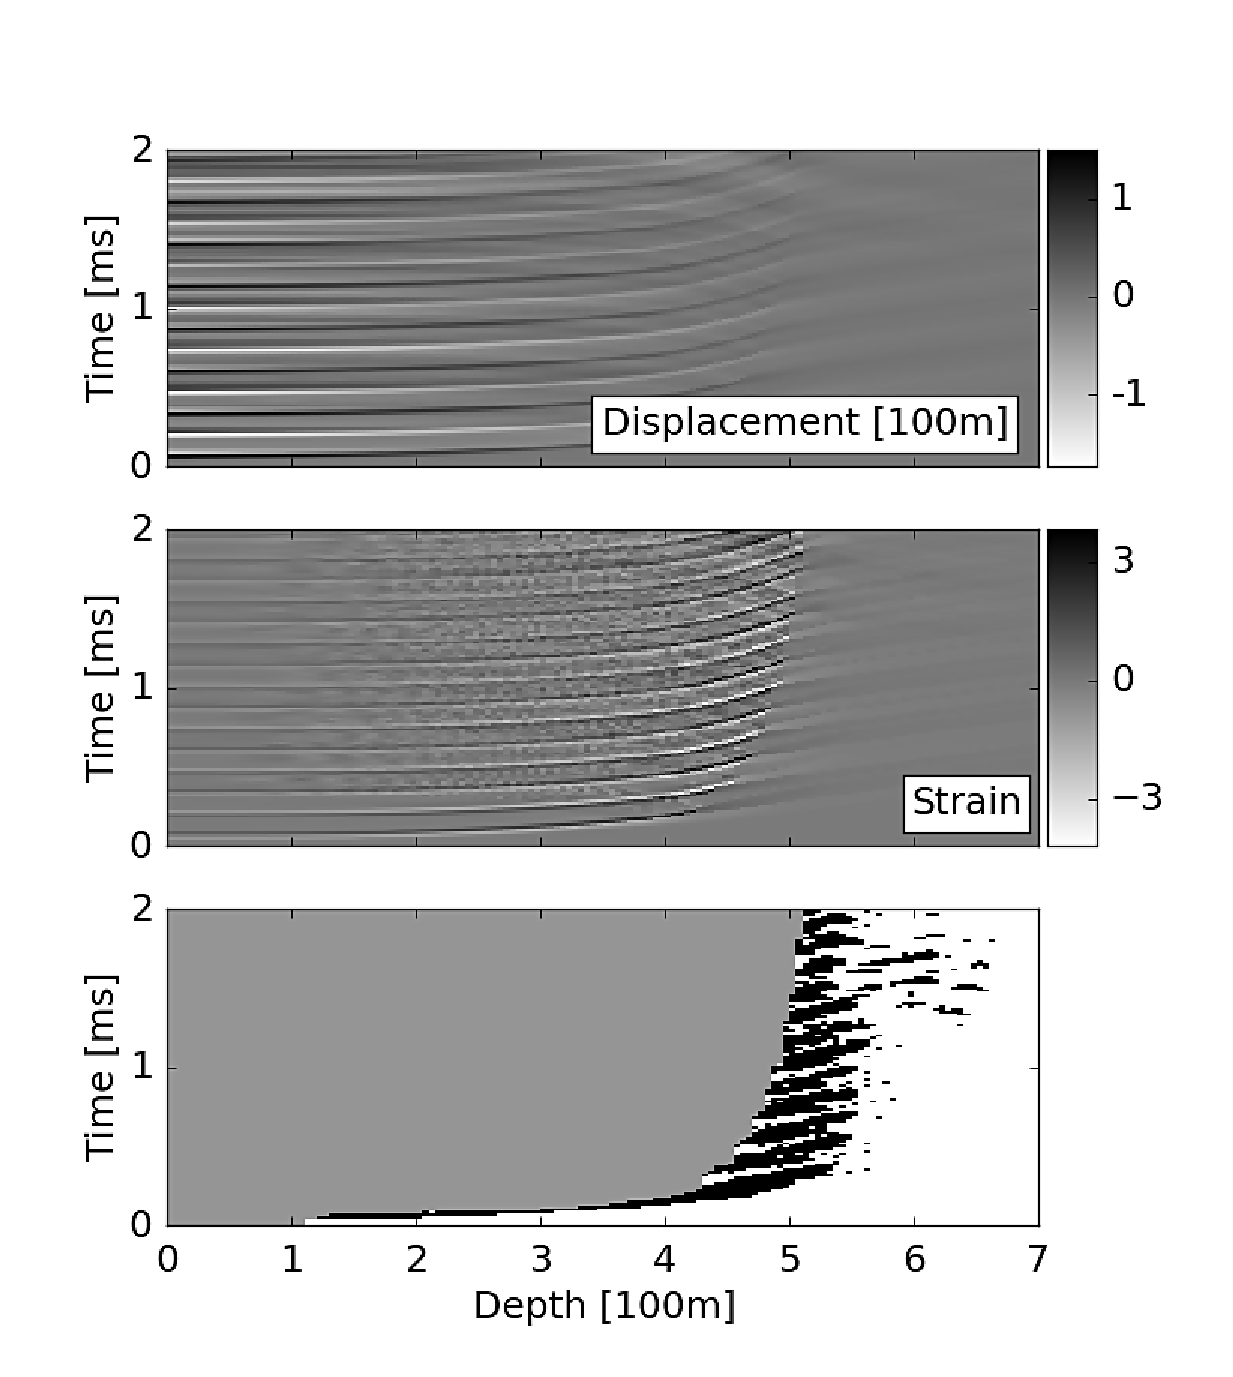
\includegraphics[width=0.6\textwidth]{pics/chap3/fig5.eps} 
\caption[Shear wave propagation in the magnetar crust viewed on the spacetime 
diagram]{Shear wave propagation in the magnetar crust viewed on the spacetime diagram: Upper panel: horizontal displacement of the wave, $\xi$. 
Middle panel: strain $s=\partial\xi/\partial z$.
Lower panel shows where the crust is deformed elastically (white), flowing plastically (black), and melted (gray).}
\label{fig5}
\end{figure}
%%%%%%%%%%%%%%%%%%

Figure~\ref{fig6} shows the history of the wave energy transmission from the magnetosphere to the crust and the plastic damping effect. 
One can see that most of the transmitted wave energy is promptly converted to heat. We have verified that our numerical simulation satisfies the conservation law (\Eq~(\ref{eq:energy})) with accuracy better than 1\%. 
Each time the wave hits the surface, the transmission coefficient is approximately 12\%, and almost all the wave energy $E_0$ is damped after $\sim 10$~ms, so most of $E_0$ becomes stored as crustal heat. 
This heating results in deep melting of the crust, down to 500~m.
%%%%%%%%%%%%%%%%%%
\begin{figure}[h]
\centering
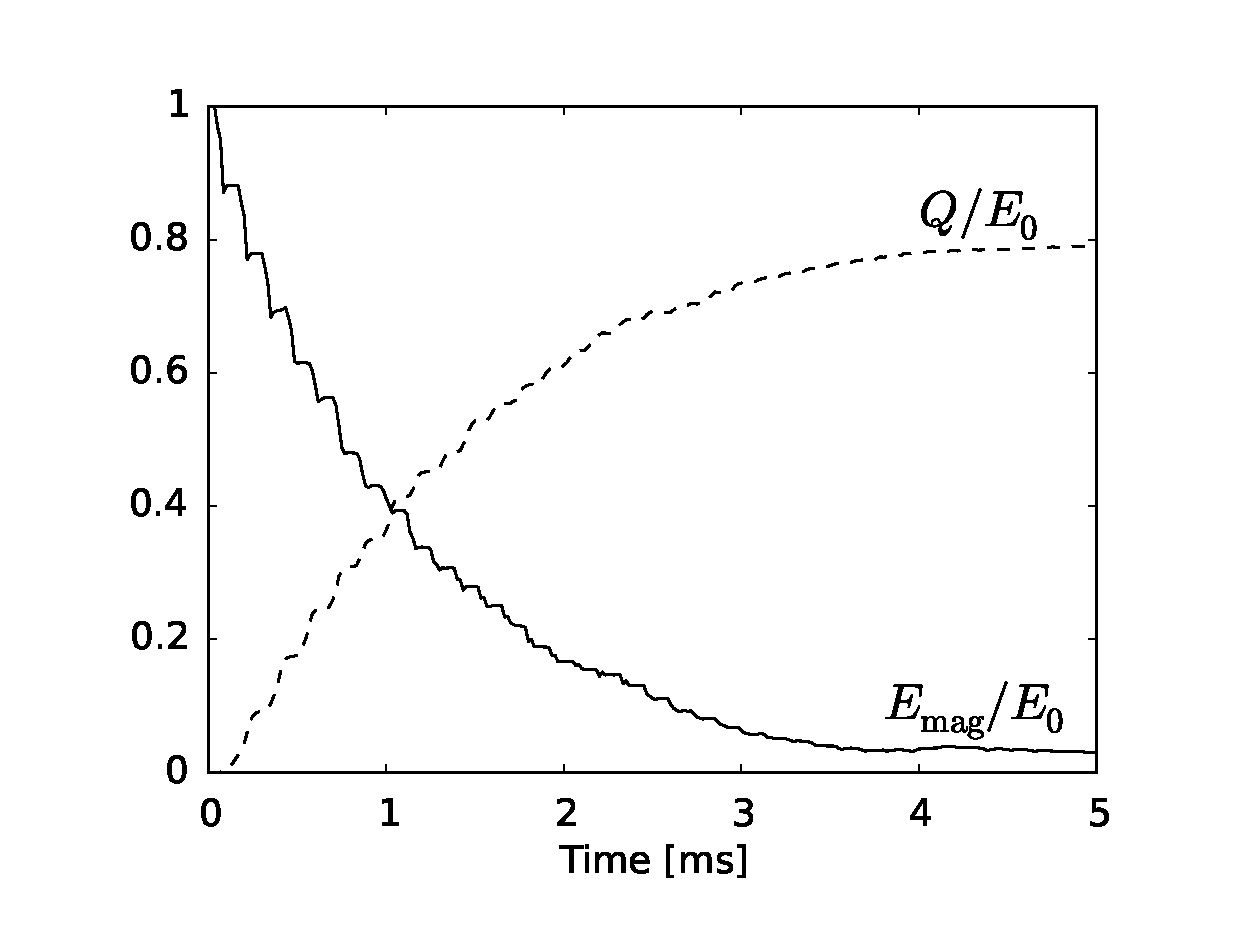
\includegraphics[width=0.6\textwidth]{pics/chap3/fig6.eps} 
\caption[Energy evolution during the reflection of \alfven waves off the crust]{Solid curve shows the evolution of the energy fraction left in the magnetosphere and dashed curve shows the energy fraction converted to heat. 
Each step in the solid curve corresponds to the simultaneous reflection of the two 
symmetric waves bouncing in the magnetosphere in the opposite directions. 
The reflection coefficient ${\cal R}\approx 0.88$, and the magnetosphere loses 
energy as ${\cal R}^{N}$ where $N$ is the number of reflection events.
Each step takes $\LL/c=(4/30)$~ms, so $\Emag/E_0\approx 0.88^{t/0.133\rm ms}$.}
\label{fig6}
\end{figure}
%%%%%%%%%%%%%%%%%%

Since plastic dissipation switches off at the melting point, the crust naturally acquires the ``ceiling'' temperature $T\approx T_m$ in an extended region below the surface.
The resulting temperature profile immediately after the flare is shown in Figure~\ref{fig7}.
To investigate how the results depend on $B_z$ and $s_0$, we have calculated the models with $B_z/10^{14}{\rm ~G}=0.3,1,3,10$ and $s_0=0.13,0.25,0.43$. 
Stronger waves in stronger magnetic fields melt deeper layers of the crust, up to 600~m in the calculated models.
%%%%%%%%%%%%%%%%%%%%%%%%
\begin{figure} [h]
\centering
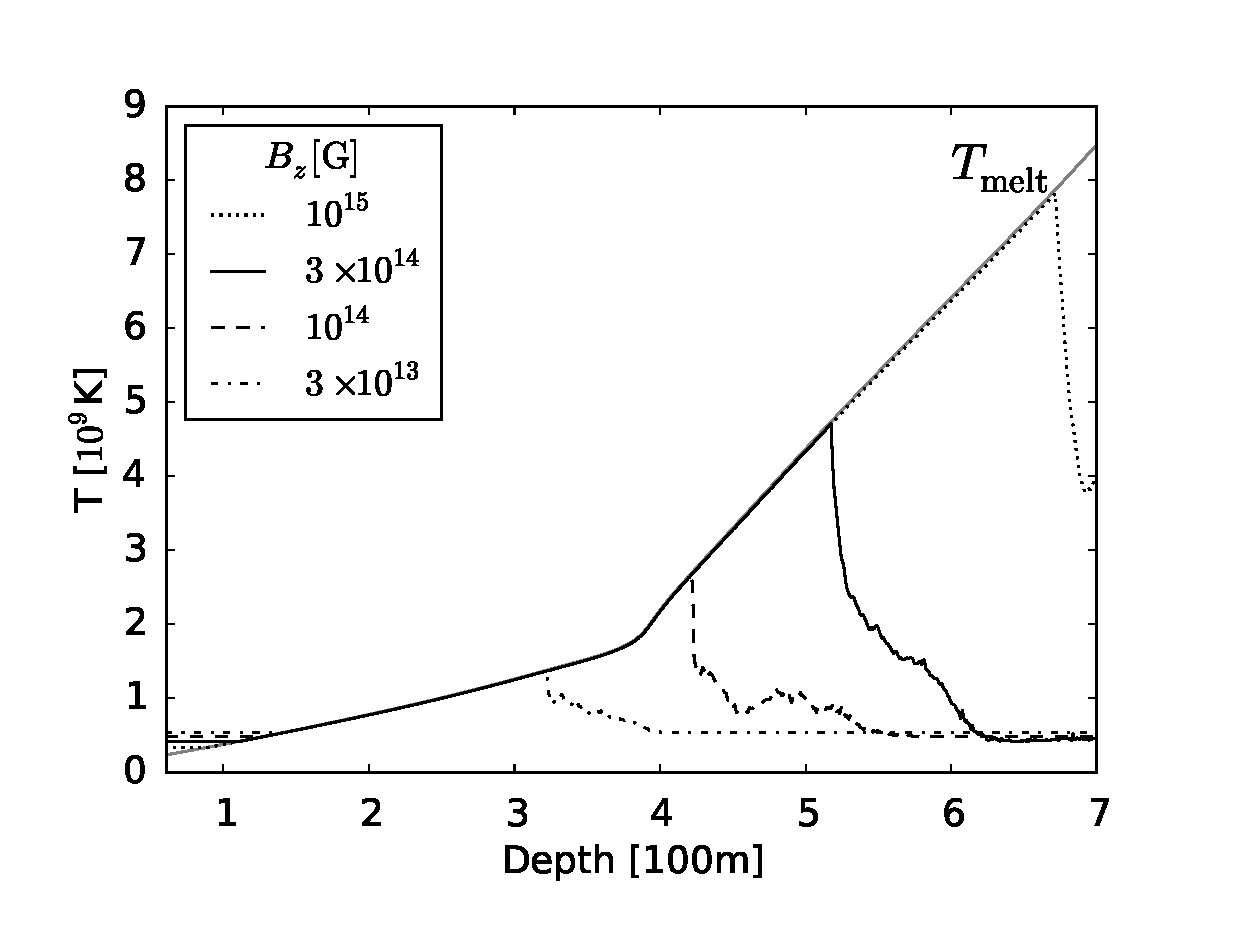
\includegraphics[width=0.48\textwidth]{pics/chap3/fig7_1.eps}
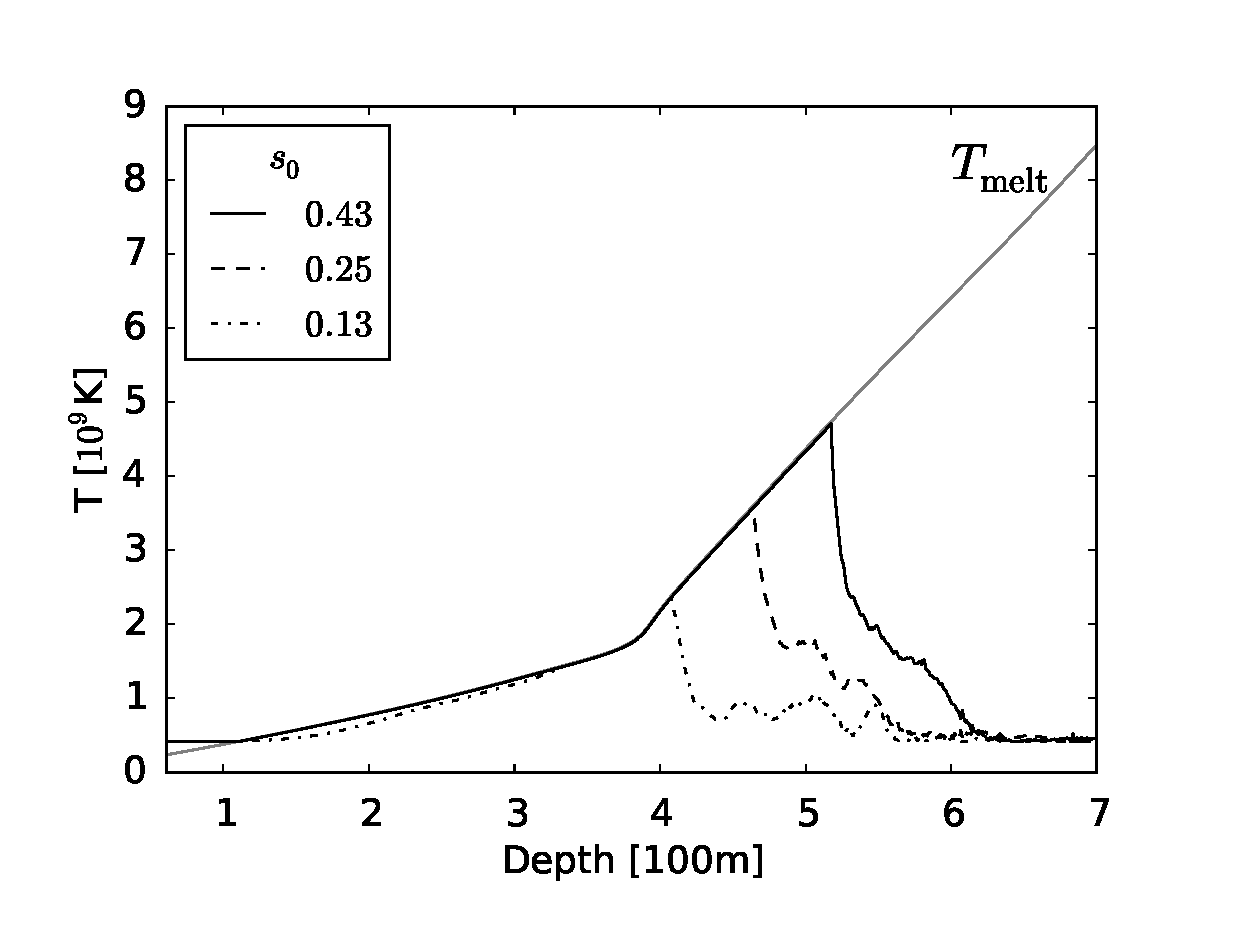
\includegraphics[width=0.48\textwidth]{pics/chap3/fig7_2.eps} 
\caption[Temperature profile after the magnetospheric \alfven waves have been 
absorbed by the crust]{Temperature profile after the magnetospheric \alfven waves have been absorbed by the crust; upper panel for fixed $s_0=0.43$ and different $B_z$, and lower panel for fixed  $B_z=3\times 10^{14}$~G and different $s_0$. 
The left boundary in the figure is chosen at depth $z\approx 60$~m where $\rho = 10^9$~g~cm$^{-3}$; at $z\lesssim 100$~m the crust is melted before the flare, and hence no plastic heating can take place.}
\label{fig7}
\end{figure}
%%%%%%%%%%%%%%%%%%%%%%%%

\section{Cooling}

After the flare, the hot crust will cool on a much longer timescale. 
Two main processes cool the crust: neutrino emission and heat conduction.
The temperature evolution with time is described by the following equation,
\begin{equation}
\label{eq:cool}
C_V \frac{\partial T}{\partial t} = 
  \frac{\partial}{\partial z}\left(\kappa
  \frac{\partial T}{\partial z}\right)-
  \dot{q}_\nu,
\end{equation}
where $\kappa$ is the thermal conductivity and $C_V$ is the heat capacity of the crust; both are functions of local $\rho(z)$, $T(z,t)$, and ${\mathbf B}$. 
The sample numerical models presented below assume a uniform vertical magnetic field $B=B_z=const$. 
We use $\kappa(\rho,T,B)$ and $C_V(\rho,T,B)$ calculated by the code of \citet{1999A&A...351..787P}. 
The term $\dot{q}_\nu(\rho,T,B)$ is the rate of local cooling by neutrino emission. This rate is described in detail by \citet{2001A&A...374..213P}. 
They provide useful analytical approximations for four relevant channels of neutrino emission: plasmon decay, bremsstrahlung, synchrotron, and electron-positron annihilation. 
We use their formulas in our calculations.

Similar to previous simulations of time-dependent heat diffusion in magnetars \citep{2006MNRAS.371..477K,2009ApJ...698.1020B,2009A&A...496..207P}, we separate the crust into two regions: a blanketing envelope and an interior region. 
Here we choose the envelope boundary at $z_b\approx 60$~m where $\rho=\rho_b=10^{9}\rm ~g/cm^3$.
The typical timescale of heat diffusion from this depth is $t_b \ll 10^6 s$.
It is sufficiently short to give a quasi-steady state in the envelope, and so the steady-state solution may be used to determine the relation between $T_b=T(z_b)$ and the effective surface temperature $T_s$.
Note that $T_s$ defines the energy flux $F=\sigma T_s^4$ through the envelope $z<z_b$, and thus in essence the $T_b$-$T_s$ relation is a relation between $T_b$ and the heat flux $F=\kappa\, \partial T/\partial z$ at $z_b$. 
It serves as a boundary condition for our time-dependent heat diffusion problem at $z>z_b$. 
Since this boundary condition relies on the steady-state solution at $z<z_b$ it can only be accurate when $T(t,z>z_b)$ evolves on timescales longer than $t_b$.

We calculated the $T_b$-$T_s$ relation at $\rho_b=10^9$~g~cm$^{-3}$ using the steady-state solutions obtained in Section~\ref{sec:steady-temp}. 
This gave a tabulated boundary condition $F(T_b)$ at the upper boundary of our computational box $z_b\approx 60$~m. 
The lower boundary is chosen at $z\approx 1$~km, near the bottom of the crust where $\rho\sim 10^{14}$~g~cm$^{-3}$. 
The exact position of the lower boundary is not important as long as it is deep enough. 
The deep crust has a high thermal conductivity and the heat is absorbed by the (approximately isothermal) core of a huge heat capacity. 
We use the absorbing boundary condition at constant temperature $T\sim 3\times 10^8$~K, neglecting the increase of the core temperature due to the absorbed heat.

The initial condition $T(z,0)$ for \Eq~(\ref{eq:cool}) is provided by the plastic heating model (Figure~\ref{fig7}). 
The initial temperature increases along the melting curve $T_m(z)$, reaches maximum, and drops at larger depths. 
We evolve this initial temperature profile on a uniform grid of 1000 points and a time step of 10~s for $10^7$ steps. 
To speed up the simulation, the values of $\kappa$, $C_V$, and $\dot{q}_\nu$ on the grid are updated every 500 time steps.
Convergence tests verified that this resolution is sufficient to obtain accurate results.
We also verified that our simulation conserves energy with better than 1\% accuracy.
The thermal energy lost by the crust is partially carried away by neutrinos and partially conducted through the boundaries.  

Figure~\ref{fig8} shows the gradual evolution of the temperature profile $T(z)$ after the flare with the fiducial parameters (see Section~2.2 and Figures~5, 6). 
During the first month, the initial peak of temperature at $z\sim 500$~m is reduced from $\sim 5\times 10^9$~K mainly due to neutrino losses. 
Then the peak continues to flatten and spread due to thermal conduction, forming a rather flat profile of $T\lesssim 10^9$~K in a few years.

%%%%%%%%%%%%%%%%%%%%%%%%
\begin{figure}[htbp]
\centering
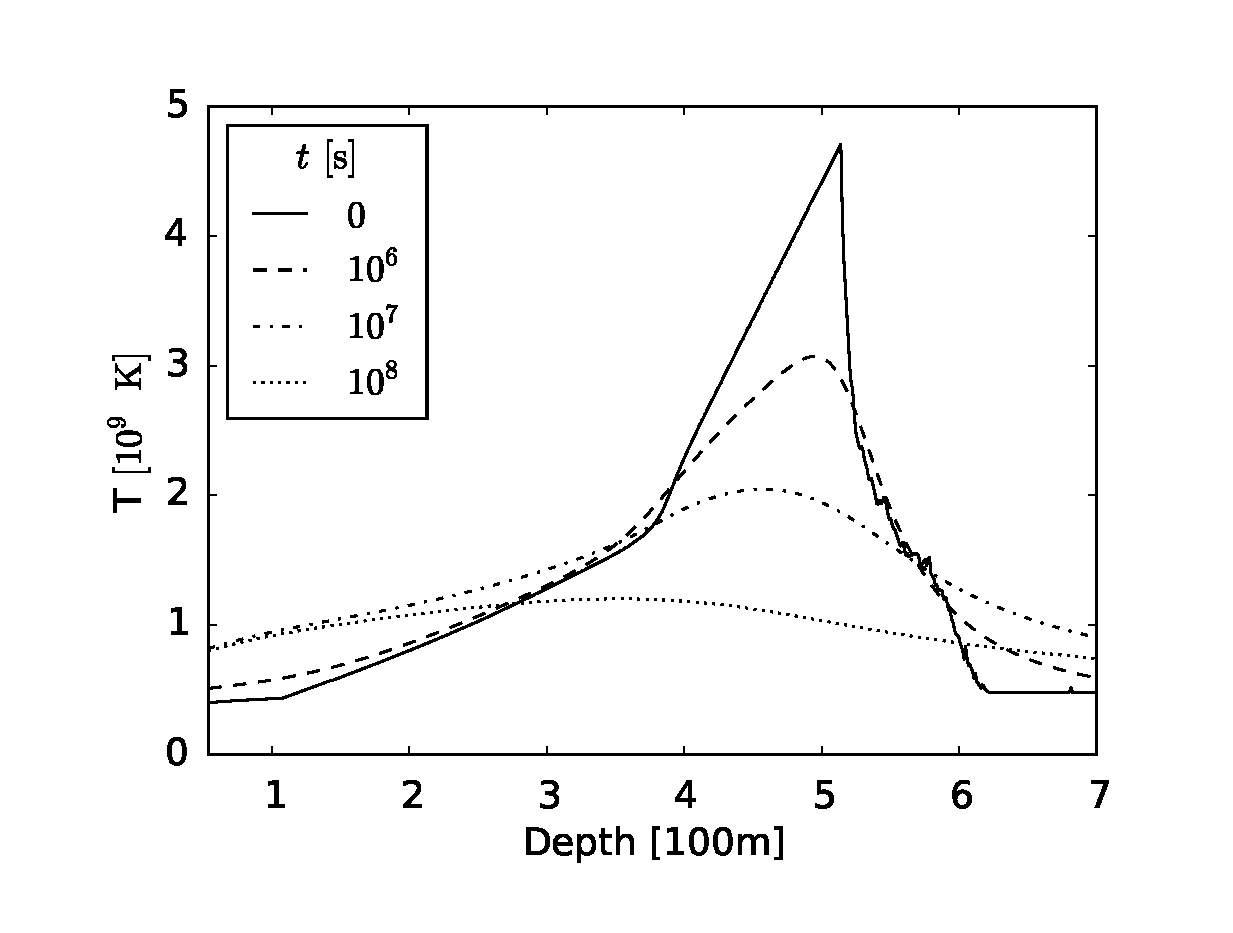
\includegraphics[width=0.6\textwidth]{pics/chap3/fig8.eps} 
\caption[Evolution of the crustal temperature profiles]{Evolution of the crustal temperature profiles in our fiducial flare model with $B=B_z=3\times 10^{14}$~G and $s_0=0.43$.}
\label{fig8}
\end{figure}
%%%%%%%%%%%%%%%%%%%%%%%%

We find that plasmon decay and bremsstrahlung make the dominant contributions to neutrino cooling, and synchrotron neutrino emission becomes significant in stronger magnetic fields $B_z\sim 10^{15}$~G. 
Electron-positron annihilation dominates neutrino cooling only in the shallow, low-density region of the crust, and its net contribution to the energy loss is negligible.

%%%%%%%%%%%%%%%%%%%%%%%%
\begin{figure}[htbp]
\centering
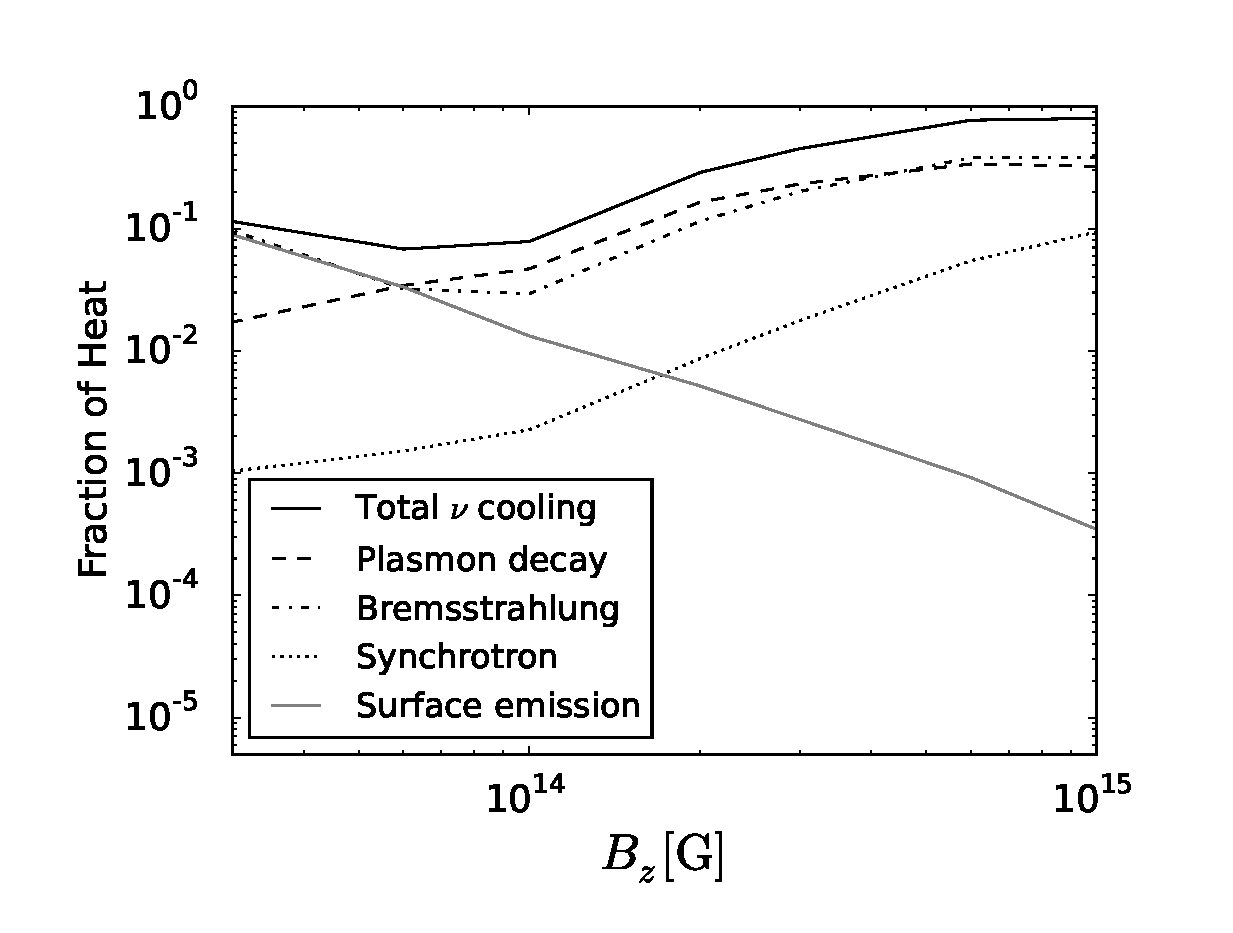
\includegraphics[width=0.6\textwidth]{pics/chap3/fig9.eps} 
\caption[Fraction of the post-flare crustal heat lost through surface emission and various channels of neutrino emission]{Fraction of the post-flare crustal heat lost through surface emission and various channels of neutrino emission, as a function of $B=B_z$. The flare is assumed to excite a pair of \alfven waves with $s_0=0.43$ which are plastically damped in the crust.}
\label{fig9}
\end{figure}
%%%%%%%%%%%%%%%%%%%%%%%%

%%%%%%%%%%%%%%%%%%%%%%%%
\begin{figure}[htbp]
\centering
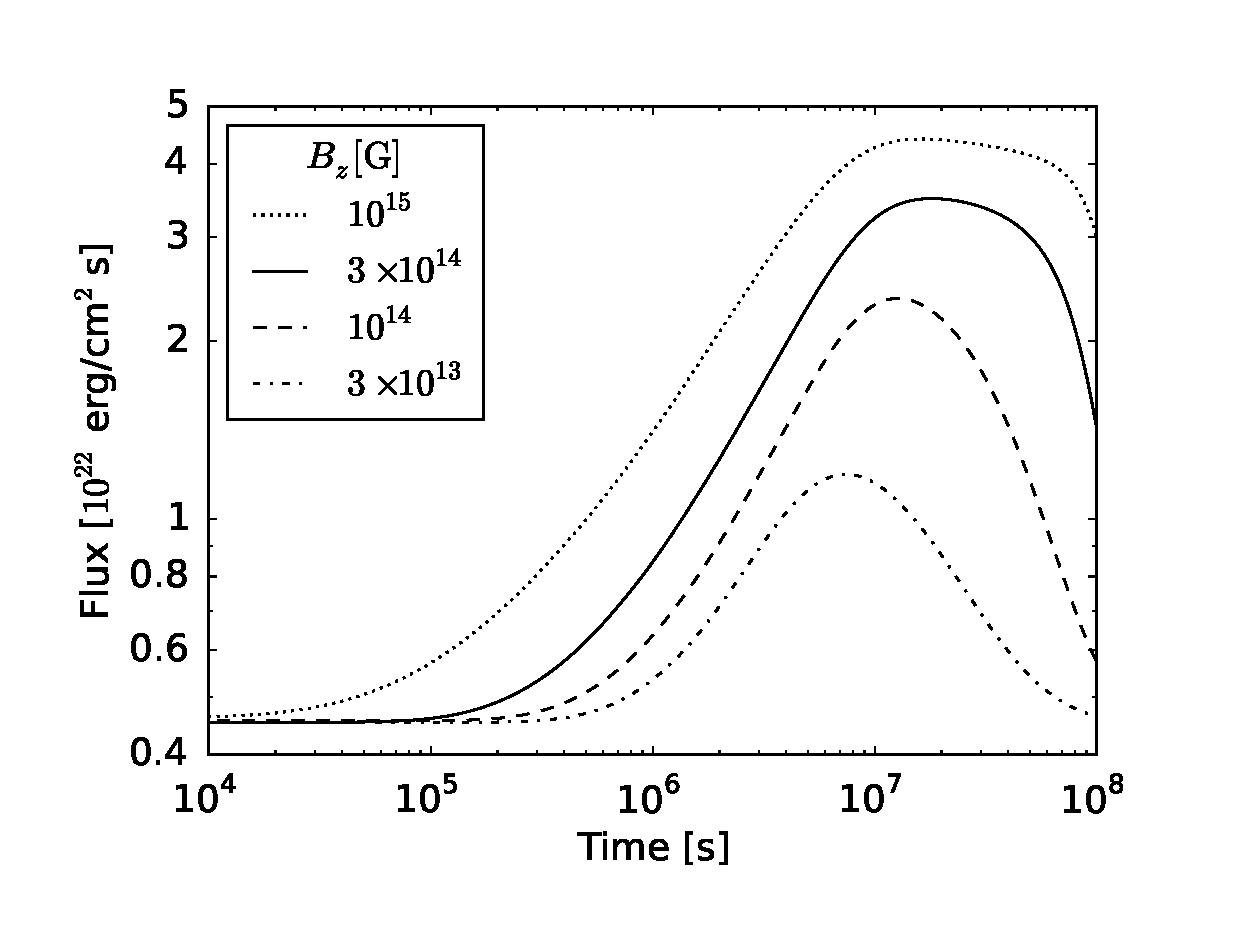
\includegraphics[width=0.48\textwidth]{pics/chap3/fig10_1.eps}
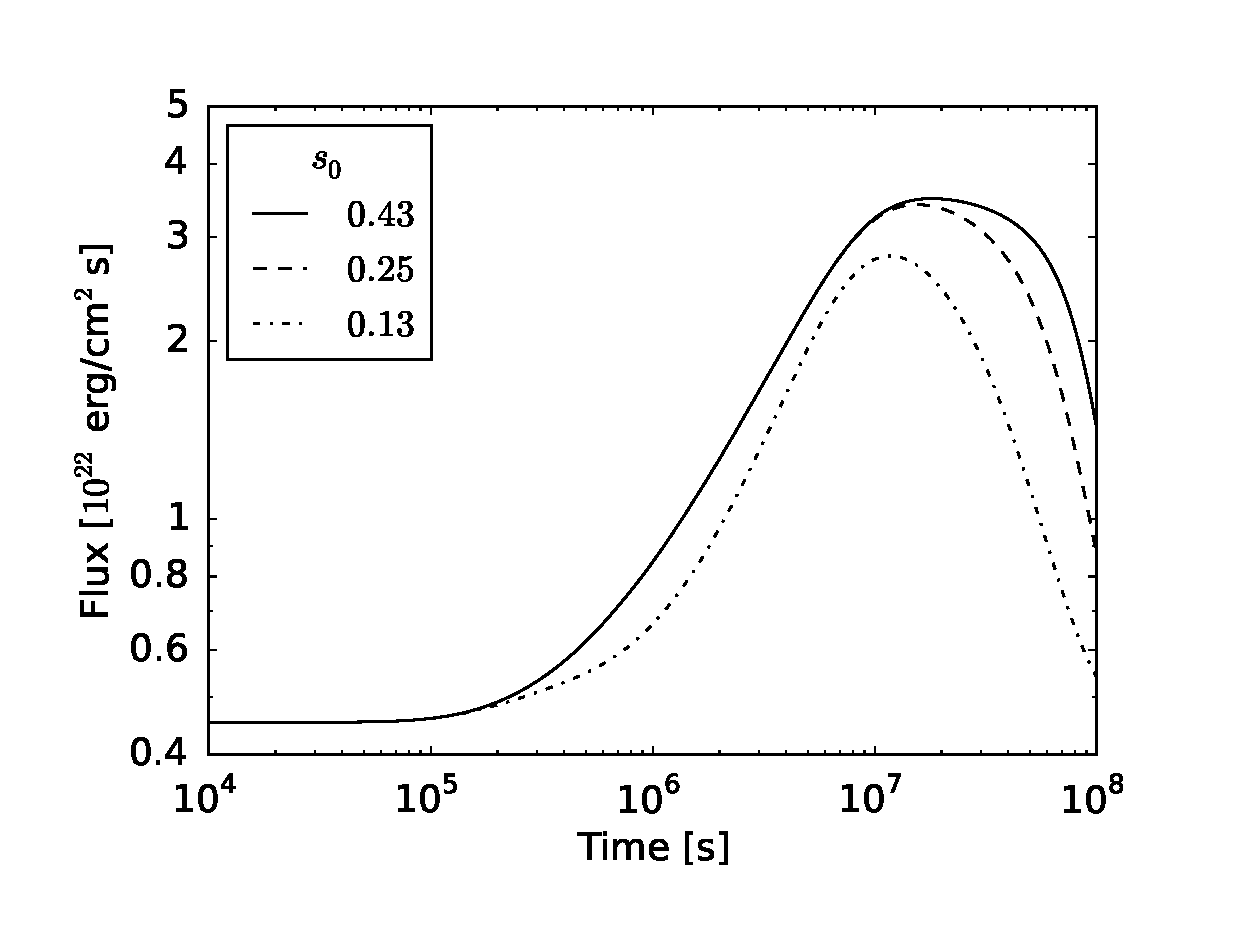
\includegraphics[width=0.48\textwidth]{pics/chap3/fig10_2.eps} 
\caption[Surface thermal flux caused by the plastic heating in the giant flare]{Surface thermal flux caused by the plastic heating in the giant flare. 
Upper panel: fixed $s_0=0.43$ and varying $B=B_z$.
Lower panel: fixed $B_z=3\times 10^{14}$~G and varying $s_0$.}
\label{fig10}
\end{figure}
%%%%%%%%%%%%%%%%%%%%%%%%

With increasing $B_z$ (and at fixed amplitude $s_0$ of the waves excited in the flare) the deposited plastic heat increases, which increases the role of neutrino cooling.
As a result, the relative contributions of plasmon decay, bremsstrahlung, and synchrotron neutrino emission depend on $B_z$. 
This dependence is shown in Figure~\ref{fig9}, where we also show the energy fraction that is conducted to the stellar surface and radiated away. 
The remaining energy fraction (not shown in Figure~9) is conducted into the core of the neutron star.

One can see from Figure~\ref{fig9} that only a small fraction of the stored crustal heat is conducted to and radiated from the stellar surface.
For example, at $B_z=3\times 10^{14}\,\rm G$ less than $1\%$ is conducted to the surface; roughly half of heat is lost neutrino emission and half is conducted to the core.

The heat radiated from the surface produces a delayed afterglow emission of the flare.
The solution of \Eq~(\ref{eq:cool}) gives the surface radiation flux $F$ as a function of time. 
This flux is shown in Figure~\ref{fig10}. 
One can see that the surface flux peaks with a significant delay after the flare --- it takes the thermal conduction timescale (of months to years) to transport the crustal heat to the surface.

The core remains much colder than the plastically heated crust. The heat conducted to the core cannot significantly boost its temperature because (1) the core has a large heat capacity, in particular if there are non-superfluid baryons \citep{2004ARA&A..42..169Y}, and (2) the core is cooled by neutrino emission, and the cooling rate quickly grows at high temperatures.

\section{Discussion}


\subsection{Plastic damping and cooling}

We described the phenomenon of plastic damping of \alfven waves 
generated in magnetar flares. Our results may be summarized as follows.

(1) {\it Transmission.}
The flare generates magnetospheric \alfven waves with energy density 
\beq
  U_0\sim \frac{\mu_B s_0^2}{2},
\eeq
where $\mu_B=B_z^2/4\pi$ is the tension of magnetic field lines, and $s_0\gtrsim 0.1$ is the shear strain of the field lines. The waves are quickly transmitted into the crust of the neutron star. 
The transmission coefficient is $\T\sim 0.1$ (Figure~\ref{fig3}), and most of the wave energy is transmitted after $N\sim \T^{-1} \sim 10$ reflection events (Figure~\ref{fig6}).
The transmitted waves form a train of $N$ oscillations propagating with velocity $v\lesssim 10^{-2}c$ and compressed by the factor of $c/v$ (Figure~\ref{fig4}).

(2) {\it Compression.}
The wave energy, which is initially spread in the magnetosphere, upon transmission becomes compressed. The energy density of the transmitted wave is
\beq 
   U_w\approx \T\, \frac{c}{v} \, U_0, 
\eeq
where $v$ decreases to $10^8$~cm~s$^{-1}$ as the wave train propagates toward the bottom of the crust. The transmission occurs at depths $z$ of a few hundred meters where the crustal density $\rho\sim 10^{10}-10^{11}$~g~cm$^{-3}$. 
In this region, $U_w$ exceeds the maximum energy that could be stored in the elastic deformation of the crust, $U_{\rm el}=\mu \scr^2/2$, and the wave propagation is still sustained by the tension of magnetic field lines, $\mu_B$. 
Therefore, the transmission also leads to the strain amplification: $s^2/s_0^2\approx U_w/U_0\sim 10$.

(3) {\it Plastic flow.}
The shear strain of the transmitted wave, $s\sim (\T c/v)^{1/2} s_0$, exceeds the maximum possible strain of elastic deformation $\scr\sim 0.1$. 
Therefore, the wave induces a strong plastic flow of the crust, which dissipates the wave energy. 
The plastic stress $\sigma$ is comparable to $\mu\scr$, which gives the dissipated energy $dq\sim \mu\scr |ds|$.
As the wave propagates into denser layers $\rho\sim 10^{12}$~g~cm$^{-3}$, the shear modulus of the lattice increases to $\mu\approx 10^{28}\rho_{12}$~erg~cm$^{-3}$ (Figure~\ref{fig1}).
The plastic heat density deposited by the wave train is given by
\beq
   \Uth \sim \sigma s N \sim \mu \scr s N.
\eeq  
The high $\Uth$ given by this estimate implies that the wave energy density $U_w$ converts to $\Uth$, i.e. efficient damping occurs.

(4) {\it Melting.}
Damping of the wave is buffered by melting --- plastic damping is inefficient where the heated crust becomes nearly liquid, and the wave continues to propagate to denser layers that have a higher $\Tm(\rho)$. 
As a result, a simple temperature profile $T\approx \Tm(\rho)$ is created by the plastic flow in an extended region of the crust (Figure~\ref{fig7}). 

Most of the wave damping occurs at depth $\zd$ where $\Tm$ is so high that the wave dissipation becomes marginally capable of melting the crust. 
Thus $\zd$ is also the depth of the melted region. At this depth the following condition is satisfied,
\beq
   C_V\Tm\sim U_w.
\eeq
We found $\zd\sim 500$~m for a typical wave energy in magnetar giant flares and $B_z\sim 3\times 10^{14}$~G (Figure~7). Deeper melting $\zd\sim 700$~m is possible if the giant flare occurs in a flux rope of a particularly strong field $B_z\gtrsim 10^{15}$~G.

(5) {\it Cooling.}
On a timescale of months to years, the deposited heat is mostly lost to neutrino emission and conducted into the core of the star (Figures~\ref{fig8} and \ref{fig9}). 
A modest energy $\Eaft$ is conducted to the stellar surface and emitted in a delayed afterglow radiation. 
A typical energy radiated per unit area is $\Eaft/S\sim 10^{30}$~erg~cm$^{-2}$.
The timescale for the rise of afterglow luminosity is the thermal conduction time $\tc\sim 10^7$~s. 
In a broad range of the flare parameters, the peak flux of surface afterglow is $F_{\max}\sim (2-4)\times 10^{22}$~erg~cm$^{-2}$~s$^{-1}$ (Figure~\ref{fig10}).

There are ways to refine our model of surface afterglow from plastic damping of magnetospheric waves. 
All sample models shown in this chapter assumed approximately vertical (radial) magnetic field in the upper crust. 
A strongly inclined field would significantly reduce thermal conductivity in the radial direction and delay the crustal cooling. 
It could also bolster a high crustal temperature before the flare, which would give a deeper melted zone where plastic damping would be impossible. 
In this case, the flare could only cause heating of the deep crust where practically all heat is wasted to neutrino emission and inward conduction. 
Thus, a strong non-radial field component tends to reduce the expected afterglow emission.

Our presented models assumed iron composition of the blanketing envelope. Light element composition of the envelope would increase its thermal conductivity \citep{2003ApJ...594..404P}, decreasing the internal temperature and reducing the depth of the melted layer in the pre-flare crust. 
Therefore, if magnetars have a light element envelope, their post-flare cooling occurs faster. 
This effect somewhat increases the afterglow flux, especially at early times, and may offset the opposite effect of the non-radial magnetic field.


\subsection{Other mechanisms of \alfven wave damping}

Nonlinear interactions of \alfven waves in the magnetosphere provide an additional damping mechanism. The existing estimates \citep{1998PhRvD..57.3219T} suggest that this mechanism will be dominant at very high amplitudes of the waves, $s_0\lesssim 1$.
The nonlinear interactions occur as the \alfven waves bounce from the stellar surface and collide in the magnetosphere. The nonlinear terms in the electrodynamic equations show two types of wave interactions: 

\noindent
(1) $A+A\rightarrow F$: two \alfven waves $A$ convert into a fast magnetosonic 
wave $F$ (which may escape the magnetosphere). 
The damping of \alfven waves by this ``3-wave'' interaction occurs on the timescale,
\beq
\label{eq:3wave}
  t_{\rm damp}\sim \frac{\lambda/c}{(k_{\bot}\xi)^2}\sim 
   \left(\frac{k_\parallel}{k_\perp}\right)^2\,\frac{\lambda/c}{s^2},
\eeq
where $\lambda=2\pi/k_\parallel$ is the wavelength along ${\mathbf B}$ (comparable to the length of the magnetospheric field line $L$), $\xi$ is the characteristic displacement in the waves, and $k_\perp$ is the wavevector component perpendicular to the magnetic field. 
The \alfven waves ducted along the curved magnetic field lines may be 
expected to have $k_\perp\sim k_\parallel$.
  
 \noindent
(2)  $A+A\rightarrow A+A$:  two \alfven waves generate two new \alfven waves. 
This ``4-wave'' interaction initiates a cascade to high $k_\perp$, which may lead to the wave dissipation on small scales \citep{1998PhRvD..57.3219T}.
The damping time due to this higher-order process is 
\beq
 \label{eq:4wave}
  t_{\rm damp}\sim \frac{\lambda/c}{(k_{\bot}\xi)^4}
     \sim  \left(\frac{k_\parallel}{k_\perp}\right)^4 \frac{\lambda/c}{s^4}.
\eeq
The time $t_{\rm damp}$ given by \Eqs~(\ref{eq:3wave}) and (\ref{eq:4wave}) should be compared with $\T^{-1}\LL/c\sim 10 \LL/c$, the lifetime of the \alfven waves to transmission and plastic damping in the crust. 
The numerical coefficients in \Eqs~(\ref{eq:3wave}) and (\ref{eq:4wave}) have not been calculated, however the estimates suggest that if the flare generates $s_0\gtrsim 1$, the nonlinear wave interactions can reduce $s_0$ to a value $\lesssim 1$ before the waves are damped plastically in the crust.
 
The wave cannot be completely damped by the plastic mechanism. 
In particular, at strains $|s|<\scr$ it propagates with no significant damping. 
The residual wave train will reach the bottom of the crust and enter the liquid core. 
It will travel through the core along the magnetic field lines and after time $\sim 2r/v$ (typically shorter than 1~s) the train will again emerge somewhere at the bottom of the crust and continue to propagate upward.

The low-amplitude waves will continue to travel through the magnetosphere and the star for a while. Their lifetime at any given amplitude $s$ is limited by the nonlinear interactions in the magnetosphere $t_{\rm damp}\propto s^{-2}$. 
The \alfven waves are also subject to gradual ohmic dissipation, as their propagation involves excitation of electric currents demanded by $\nabla\times{\mathbf B}\neq 0$.
After the flare, the effective resistivity of the magnetosphere is controlled by the threshold voltage of electron-positron discharge that is self-organized to conduct the electric currents \citep{2007ApJ...657..967B}.

\subsection{Observed afterglow}

Sudden crustal heating followed by gradual crustal cooling was proposed to power the afterglow of the giant flare in SGR~1900+14 \citep{2002ApJ...580L..69L}.
The afterglow was extremely bright in the first hours after the flare, $\Lum\sim 10^{37}-10^{38}$~erg~s$^{-1}$, and during the next month it showed a power law decay $\Lum\propto t^{-0.7}$ \citep{2001ApJ...552..748W}.
\citet{2002ApJ...580L..69L} explored how heat should be deposited to give the observed afterglow light curve and found that heating should be approximately uniform throughout the 500-m-deep layer below the surface. 
This implies, in particular, enormous heating in the shallow layers $z\ll 100$~m. 
The heating mechanism in the low density layers is unclear and certainly cannot be provided by plastic dissipation. 
Therefore we do not attempt to explain the early afterglow of SGR~1900+14 by crustal heating.
We also note that the afterglow spectrum was nonthermal \citep{2001ApJ...552..748W}, which suggests a magnetospheric source. 

Plastic damping of magnetospheric \alfven waves produces a well defined temperature profile  of the crust: $T\approx \Tm(z)$ down to $\zd$. This leads to specific predictions for the afterglow light curves (Figure~10), with the surface flux $F\sim (2-4)\times 10^{22}$~erg~cm~$^{-2}$~s$^{-1}$ on a timescale $\gtrsim 100$~d. 
This flux and timescale appear to be consistent with observations of some less energetic ``transient'' magnetars after their bursting activity.

In particular, the luminosity of SGR~1627-41 after its outbursts in 1998 and 2008 showed a decay on a year timescale \citep{2006A&A...450..759M,2008MNRAS.390L..34E,2012ApJ...757...68A}. 
The luminosity at $t\sim 100$~d was $\Lum\sim 7\times 10^{34}(d/11{\rm ~kpc})^2$~erg~s$^{-1}$ after the 1998 outburst and $\Lum\sim 2\times 10^{34}(d/11{\rm ~kpc})^2$~erg~s$^{-1}$ after the 2008 outburst, where the distance $d\approx 11$~kpc was inferred from the apparent location of SGR~1627-41 in a star-forming region (Hurley et al. 1999). 
The decay on a year timescale is consistent with the crust melting down to $\zd\sim 300$~m, and the observed luminosity $\Lum$ is consistent with the melted crust area occupying $\sim 10$\% of the stellar surface.

Swift~J1822.3-1606 provides another example. It produced afterglow emission following the outburst in 2011 \citep{2012ApJ...754...27R,2012ApJ...761...66S,2014ApJ...786...62S}.
Similar to the afterglow of SGR~1627-41, its light curve may be described as a double exponential, with the second (longer) exponential component visible after $\sim 100$~d. 
\citet{2014ApJ...786...62S} used a crustal cooling model to describe both the early and late afterglow components in Swift~J1822.3-1606. In their model, heat deposition is a phenomenological parameter adjusted to reproduced observations. 
We find that plastic damping of magnetospheric waves is only capable of explaining the late afterglow component, and the early component must invoke a different heat source.
The late component has the luminosity and decay timescale similar to those observed in SGR~1627-41, consistent with the crust melting down to $\zd\sim 300$~m.

A reliable identification of the crustal afterglow is complicated by the presence of another, {\it nonthermal}, emission component. The nonthermal source is likely present during the afterglow of SGR~1627-41 \citep{2012ApJ...757...68A}, and nonthermal hard X-rays are unambiguously detected in the transient magnetar 1E~1547.0-5408 during its afterglow following the 2009 outburst \citep{2012MNRAS.427.2824E,2012ApJ...748..133K}.
The nonthermal activity is usually associated with the twisted equilibrium magnetosphere, which carries persistent electric currents \citep{2002ApJ...574..332T,2013ApJ...762...13B}. 
The twist is ohmically dissipated over a year timescale, which happens to be comparable to the timescale of crustal cooling.

Another complication is the expected {\it external} heating of the stellar surface bombarded by magnetospheric particles. This heating occurs at the footprint of the current-carrying magnetic field lines (``j-bundle''). 
As the magnetosphere slowly untwists, the j-bundleshrinks and so does its hot footprint \citep{2009ApJ...703.1044B}. 
Such shrinking hot spots have been observed in several transient magnetars, including the canonical transient magnetar XTE~J1810-197. 
Following an outburst in 2003 it showed an X-ray afterglow decaying on a year timescale, with luminosity $\Lum\sim 2\times 10^{34}$~erg~s$^{-1}$ at $t\sim 1$~yr \citep{2007Ap&SS.308...79G}. 
The observed area $A(t)$ and luminosity $\Lum(t)$ of the hot spot evolved in agreement with the predictions of the untwisting magnetosphere model. 
Similar shrinking hot spots were observed in 1E~1547.0-5408, CXOU~J164710.2-455216, SGR~0501+4516, SGR~0418+5729 (see the data collection in \citet{2011heep.conf..299B} and references therein) and more recently in Swift~J1822.3-1606 \citep{2014ApJ...786...62S} and the Galactic Center magnetar SGR~J1745-2900 \citep{2015MNRAS.449.2685C}.

Strong \alfven waves and deep plastic heating are certainly expected in energetic events, in particular in giant flares. All three giant flares observed to date were emitted by persistently active magnetars, which maintain a high level of both magnetospheric activity and surface luminosity. It is possible that plastic damping of \alfven waves is the main mechanism that keeps the crust hot in these objects.

% Local Variables:
% TeX-master: "../thesis"
% zotero-collection: #("16" 0 2 (name "Thesis"))
% End:

\zotelo{../thesis.bib}

\chapter[Dissipation of Alfv\'{e}n Waves in Magnetar Magnetospheres]{Dissipation of Alfv\'{e}n Waves in Magnetar Magnetospheres}
\label{chap:magnetosphere-dissipation}

Giant flares of magnetars are likely powered by a sudden magnetospheric rearrangement that dissipates magnetic energy \citep{1995MNRAS.275..255T,1996ApJ...473..322T,2001ApJ...561..980T}.
A slower mode of dissipation is invoked to explain persistent hard X-ray emission \citep{2013ApJ...762...13B}.
Magnetic energy dissipation in the magnetosphere generally plays a key role in magnetar activity.

One proposed dissipation mechanism is the turbulent cascade of magnetospheric \alfven waves excited by a starquake \citep{1996ApJ...473..322T}. \alfven waves are also excited when the magnetosphere is slowly ``overtwisted'' and loses equilibrium, as observed in simulations by \citep{2013ApJ...774...92P}. The excited waves can have large amplitudes and carry a significant fraction of the magnetospheric energy. 

\citet{1996ApJ...473..322T,2001ApJ...561..980T} proposed that the waves will cascade to small dissipative scales and convert to heat, creating an energetic ``fireball'' of thermalized $e^\pm$ plasma. However, there are two competing processes that can remove the wave energy. First, \alfven waves can convert to so-called ``fast modes'' capable of escaping the magnetosphere. Unlike \alfven waves, which are ducted along the magnetic field lines and trapped in the closed magnetosphere, fast modes can propagate across the field lines.
Secondly, \citet{2015ApJ...815...25L} showed that \alfven waves bouncing in the magnetosphere are gradually drained into the stellar crust, where they initiate plastic flows and dissipate. About 10 bouncing cycles are typically sufficient to damp the waves by this mechanism, and \citet{2015ApJ...815...25L} suggested that this may occur faster than dissipation of waves through a turbulent cascade in the magnetosphere. Evaluating the efficiency of the latter process requires a detailed calculation of nonlinear processes, which can be done numerically. We attempt this calculation in the present chapter.

The theory of turbulent cascades has a long history. The MHD cascade is different from the hydrodynamic cascade where energy transfer is mediated by interacting vortices. The difference is seen already in the simplest, incompressible, non-relativistic MHD, where only \alfven waves are present. In the case of weak turbulence (meaning that the time for energy transfer across spatial scales is longer than the wave period),
the three-wave interaction is prohibited by kinetic constraints \citep{1994ApJ...432..612S}. 
Then nonlinear interactions are dominated by the four-wave interactions among \alfven waves and give rise to the anisotropic energy cascade in the direction perpendicular to the background field. For strong turbulence, a $k_\perp^{-5/3}$ spectrum was predicted from detailed balance \citep{1995ApJ...438..763G}.

More work was done later to include compressive modes -- the fast and slow magnetosonic waves.
Using the random phase approximation \citet{2001JETP...93.1052K} found a weak-turbulence spectrum $k_{\perp}^{-2}$.
Relativistic nonlinear Alfv\'enic turbulence was studied using numerical simulations \citep{2005ApJ...621..324C,2012ApJ...744...32Z,2016ApJ...817...89Z,2016ApJ...831L..11T,2017MNRAS.472.4542T}, but far less than in the non-relativistic setting. 
Simulations by \citet{2016ApJ...831L..11T,2017MNRAS.472.4542T} suggested that compressible modes are strongly coupled with \alfven waves and participate in the energy cascade.

Similar to the previous works, we are interested in low-frequency waves, which are described by relativistic magneto-hydrodynamics (RMHD). In the magnetically-dominated limit (negligible plasma inertia), a simpler approximation of ``force-free electrodynamics'' (FFE) becomes useful. In this approximation, the plasma energy and momentum are neglected and the stress-energy tensor of the electromagnetic field $T^{\mu\nu}$ satisfies $\nabla_\mu T^{\mu\nu}=0$.
Both RMHD and FFE support \alfven waves, which transport energy along the direction of the background field, and also support the fast modes.\footnote{In FFE, name ``fast'' is somewhat misleading, because all waves propagate with the speed of light.}

An analytical study of wave interaction in FFE by \citet{1998PhRvD..57.3219T} found that an \alfven wave pair can convert to a fast wave via three-wave interactions. 
In contrast to \alfven waves, the group velocity of the fast modes can be in any direction and they can possibly escape the magnetosphere, carrying energy away.

In this chapter we use FFE and RMHD simulations to investigate the efficiency of nonlinear processes in removing wave energy through dissipation and escape.
Our goals are to determine the fate of wave energy in the context of giant magnetar flares, and to study the nonlinear dynamics of interacting \alfven waves from a physics perspective.
We present numerical simulations of relativistic \alfven wave turbulence operating in a toy magnetosphere replaced by a rectangular box.
We utilize a high-order conservative finite differencing scheme to evolve the FFE equations, and devote particular attention to the code's modeling of energy dissipation. We discuss the various modes by which energy is removed numerically, and point out (via direct comparison with a relativistic MHD code) circumstances when FFE wrongly models the energy dissipation rate.

We will outline our numerical scheme and discuss energy dissipation channels it admits and present 2D and 3D numerical results for \alfven wave turbulence driven by colliding wave packets. 
We will show that FFE simulations can badly over-predict the energy dissipation rate, as the result of a commonly employed technique for maintaining magnetic dominance ($E < B$) and discuss our results in the context of the fireball model for magnetar giant flares. 
Throughout this chapter we utilize units in which speeds are measured in units of the speed of light $c$, and electric ($\boldsymbol{E}$) and magnetic ($\boldsymbol{B}$) field values are normalized by $\sqrt{4 \pi}$.

\section{Numerical setup}
\subsection{Computational setting}
%
We perform numerical simulations in a fully periodic domain with uniform guide magnetic field aligned with the $z$-axis, $B_z=1$.
The box extends from -0.5 to 0.5 along each axis, and the wave crossing time is also unity.
We utilize initial conditions comprising a pair of counter-propagating \alfven wave packets.
Due to the use of periodic boundary conditions, the wave packets collide repeatedly, twice each time they traverse the computational domain; the time interval between successive collisions is $\tau = 0.5$.
This setting simulates \alfven wave packets propagating on closed field lines anchored on the magnetar surface, neglecting geometric effects due to the field-line curvature. The periodic boundary condition corresponds to an idealized situation where \alfven waves are perfectly reflected when hitting the magnetar surface.

\subsection{Solution scheme}
\label{scheme}
%
We numerically evolve the FFE equations (Equations~\ref{eq:Maxwell} and \ref{current}) using a third-order in time, fifth-order in space, flux-conservative scheme based on the WENO method \citep{doi:10.1137/070679065} adapted to FFE \citep{2011MNRAS.411.2461Y}.
We define a vector of primitive variables,
%
\begin{equation}
	\bp= \left(B_x,B_y,B_z, E_x,E_y,E_z\right)^\top \, ,
\end{equation}
%
and rewrite the Maxwell equations in the flux-conservative form
%
\begin{equation} \label{maxwell-fv}
	\partial_t \bp + \partial_x\bF^x + \partial_y\bF^y + \partial_z\bF^z = \boldsymbol{T} \, ,
\end{equation}
%
where the source term $\boldsymbol{T}$, and the flux functions are given by
%
\begin{eqnarray}
	\boldsymbol{T} &=& \left(0,0,0, -J_x, -J_y, -J_z\right)^\top \nonumber\\
	\bF^x &=& \left(0,-E_z,E_y,0,B_z,-B_y\right)^\top \nonumber\\
	\bF^y &=& \left(E_z,0,-E_x,-B_z,0,B_x\right)^\top \nonumber\\
	\bF^z &=& \left(-E_y,E_x,0, B_y,-B_x,0 \right)^\top \, .
\end{eqnarray}
The components of electric current appearing in $\boldsymbol{T}$ are computed using standard forth order finite differencing on the volume-centered values of $\be$ and $\bb$, according to Equation \ref{current}.

Time stepping is accomplished using the third-order TVD Runge-Kutta (RK) method \citep{Gottlieb:1998:TVD:279724.279737}.
Each RK sub-step updates the primitive variables by adding the source term and face-centered fluxes in a finite-volume form of Equation \ref{maxwell-fv}
%
\begin{equation}
    \bp^{n + 1} = \bp^n + \boldsymbol{T}^n \Delta t - \frac{\Delta t}{\Delta V} \sum_{\rm{faces}} \Delta S_i \hat{\boldsymbol{F}}^i\, .
\end{equation}
%
Here $\hat{\boldsymbol{F}}^i$ are the face-centered fluxes, evaluated from $\bp^{n}$, and Roe's Riemann solver,
%
\begin{eqnarray}
	\hat{\bF}^i_{j+1/2} &=& \frac{1}{2}\Big[\bF^i(\bp^+_{j+1/2}) + \bF^i(\bp^-_{j+1/2}) \nonumber\\
    && -\sum\limits_{m=1}^6  \left|\lambda^i_{m, j+1/2}\right| \alpha^i_{m, j+1/2}\boldsymbol{v}^i_{m, j+1/2} \Big]
\end{eqnarray}
%
where  $\lambda^i_{m, j+1/2}$ and $\boldsymbol{v}^i_{m, j+1/2}$ are eigenvalues and eigenvectors of the Jacobian matrix $\partial \bF^i / \partial \bp$,
%
and
%
\begin{equation}
	\alpha^i_{m, j+1/2,j,k} = \left(\bp^+_{j+1/2}-\bp^-_{j+1/2}\right) \cdot \boldsymbol{v}^i_{m, j+1/2}
\end{equation}
%
is the projection of the difference between left and right states to the eigenvectors.
The left and right states $\bp^{\pm}$ are reconstructed from $\boldsymbol{P}^n$ using the fifth order WENO method. 

\subsection{Constraint preservation}
\label{constraint}
%
In order to keep the magnetic field divergence-free, we utilize the hyperbolic divergence cleaning approach outlined in \citet{2002JCoPh.175..645D}. In practice, we find this approach maintains $\nabla \cdot \bb = 0$ to high precision. Note that violations in $\nabla \cdot \bb = 0$ only arise from the truncation error of the numerical scheme, and so the modifications to the solution introduced by the hyperbolic cleaning step converge away with increasing numerical resolution. Hyperbolic divergence cleaning involves the addition of an auxiliary scalar field $\Psi$ and a corresponding evolution equation. For brevity, we have excluded this equation from the description of our numerical scheme in Section \ref{scheme}. For details we refer the reader to \cite{2002JCoPh.175..645D}.

Small violations in the $\be \cdot\bb = 0$ constraint also arise at the level of truncation error. Instead of removing the parallel component of $\be$ at each time step, we introduce a correction term to the force-free Ohm's law that allows for time-resolved damping of $\be_\parallel$ \citep{2017MNRAS.469.3656P},
%
\begin{eqnarray} \label{modified-ffe-ohm}
		\bj_m &=& \rho_e \frac{\be\times\bb}{B^2 +\tilde{E}^2} \nonumber\\
		 && + \frac{\bb\cdot\nabla\times \bb - \be\cdot\nabla\times\be + \gamma \be\cdot\bb}{B^2}\bb \, .
\end{eqnarray}
%
Here, $1 / \gamma$ is a time scale for the damping of $\be_\parallel$ (typically chosen to be several times $\Delta t$), and the modified electric field magnitude $\tilde E^2$ appearing in the denominator of the first term in Equation \ref{modified-ffe-ohm} is defined as \citep{2012ApJ...746...60L}
%
\begin{equation}
	\tilde{E}^2 = \frac{1}{2} \left(\sqrt{\chi^4 + 4 \be \cdot \bb} + \chi^2\right) - \chi^2 \, ,
\end{equation}
%
where $\chi^2 \equiv B^2 - E^2$.
When $\be \cdot \bb = 0$, the modified current density Equation \ref{modified-ffe-ohm} reduces to Equation \ref{current}.


\subsection{Maintaining magnetic dominance}
\label{magnetic-dominance}
%
Self-consistent evolution of the FFE equations requires magnetic dominance ($E < B$) to be maintained. However, non-linear FFE solutions in which $E$ remains everywhere smaller than $B$ generally exist only for finite time. This reflects that realistic plasma systems, having small but finite rest-mass energy, inevitably develop regions where the thermal pressure gradient or the MHD inertial term becomes important.
Such conditions arise either where $B^2 / 2$ drops below $\rho$ (e.g. near magnetic null points), or where plasma is accelerated to high Lorentz factor. In such regions the electric current deviates significantly from $\bj_{\rm FFE}$, enabling momentum transfer between the plasma and the electromagnetic field. 

A standard procedure to continue numerical evolution of the FFE equations is to artificially reduce the magnitude of $E$ wherever $E > B$,
%
\begin{equation}\label{shrinkE}
	\be\rightarrow\sqrt{\frac{B^2}{E^2}} \be \, .
\end{equation}
%
This procedure is commonly interpreted as modeling a dissipative process \citep{2006MNRAS.367.1797M, 2006ApJ...648L..51S}, such as the rapid acceleration of charged particles enabled by $E > B$. However, violation of the force-free condition in real plasma systems does not necessarily lead to energy dissipation. We will demonstrate this explicitly in Section \ref{sec:breakffe} by comparing our FFE solutions with those of strongly magnetized relativistic MHD. The MHD solutions reveal that breaking of the force-free condition leads to time-reversible momentum exchange between the field and the plasma. We will thus conclude that electromagnetic dissipation is not properly modeled by FFE when significant energy is lost as a consequence of the procedure in Equation \ref{shrinkE}.

\subsection{Dissipation channels in FFE simulations}
\label{dissipation-channels}
%
Although FFE formally conserves energy, numerical evolution schemes require some dissipation in order to maintain stability, satisfy constraints, and keep the solution magnetically dominated. There are four channels for energy dissipation in our numerical simulations:
%
\begin{enumerate}[(i)]
\item The hyperbolic divergence cleaning step, which leads to 
\begin{equation}
		\partial_t U = -\bb \cdot \nabla \Psi \, ,
	\end{equation}
    %
	where $\Psi$ is the auxiliary scalar function discussed in Section \ref{constraint}.
    %
	\item Dissipation introduced by the modified force-free current $\bj_m$ in Equation \ref{modified-ffe-ohm}.
    %
	\begin{eqnarray}
	 \partial_t U &=& - \bj_m \cdot\be \nonumber \\ 
	                   &=& -(\be\cdot\bb)\frac{\bb\cdot\nabla\times \bb-\be\cdot\nabla\times\be}{B^2} \nonumber \\
	                   &&-\frac{\gamma (\be\cdot\bb)^2}{B^2}.
	\end{eqnarray}
	\item Reduction of electrical field when $E>B$ (Equation \ref{shrinkE}).
	\item Subtraction of short-wavelength field oscillations at the grid scale, referred to as ``grid heating.''
\end{enumerate}
%

Channels (i) and (ii) become less significant with increasing grid resolution, because the numerical values of $\Psi$ and $\be\cdot\bb$ are proportional to the truncation error of the numerical scheme. In the results presented in Sections \ref{sec:spec} and \ref{sec:fate}, these channels do not contribute significantly to the measured energy dissipation rate.

Channel (iii) does not in general become small as the grid resolution increases. 
As mentioned in Section~\ref{magnetic-dominance}, this dissipation may be artificially strong.
Therefore, we consider our measurements of the energy dissipation rate to be reliable only when dissipation is not dominated by this effect.

Channel (iv), energy removal by grid heating, may or may not ``converge away'' with increasing resolution. For example, the FFE wave solutions discussed in Section \ref{waves} evolve without any significant grid heating, provided their wavelength is well resolved. Generally, the rate of grid heating of isolated waves will depend on the numerical resolution. In contrast, non-linear numerical solutions can exhibit significant energy loss over time, at a rate that becomes independent of grid resolution. Such behavior usually reflects the presence of a forward energy cascade, in which the rate of high frequency wave damping is determined by the rate of energy transfer into high frequency modes by numerically resolved non-linear interactions. In such cases, grid heating is expected to capture the true dissipation rate.

\subsection{Numerical diagnostics}
%
A useful diagnostic in our analysis will be the free energy $U$, which we define to be the total electromagnetic energy of the system, but with the contribution from the background magnetic field $B_z$ removed,
%
\begin{equation}
	U \equiv U_{\rm tot} - \frac{1}{2} \int \md V\; B_z^2 \, .
\end{equation}
%

We will also utilize the power spectra $P(k_\parallel)$ and $P(k_\perp)$, representing the distribution of electromagnetic energy in wavenumber parallel and perpendicular to the background field. The power spectra are obtained by binning the square of the discrete Fourier modes $\tilde{\bb}(\boldsymbol{k})$ and $\tilde{\be}(\boldsymbol{k})$ by the wavenumber components $k_\parallel$ and $k_\perp$,
%
\begin{equation} \label{eqn:power-spectrum}
	P(k_{\parallel,\perp}) \Delta k_{\parallel,\perp}\equiv \frac{1}{2 U_0} \sum\limits_{\boldsymbol k \in \Delta k_{\parallel, \perp}} |\tilde{\bb}(\boldsymbol{k})|^2 + |\tilde{\be}(\boldsymbol{k})|^2 \, .
\end{equation}
%
Note that the spectra are normalized to the free energy $U_0$ in the system at $t=0$, such that
%
\begin{equation}
	U = U_0 \sum 
	P(k_\parallel)\Delta k_\parallel =
    U_0 \sum 
      P(k_\perp) \Delta k_\perp \, .
\end{equation}
In 2D and 3D runs, the spectral bins $\Delta k_\parallel$ are planar slabs orthogonal to the background field. The spectral bins $\Delta k_\perp$ are planar slabs in 2D and cylindrical annuli in 3D.
%

\section{Spectral evolution of wave turbulence}\label{sec:spec}
\subsection{3D simulations}\label{sec:3d}
%
Turbulent cascade in our simulations is generated by collisions of two counter-propagating \alfven wave packets in a uniform background magnetic field $\boldsymbol{B}_0=B_0\hat{\boldsymbol{z}}$. 
The initial packets occupy two spherical volumes centered at $\boldsymbol{r}_1 = (0,0,-0.25)$ and $\boldsymbol{r}_2 = (0,0,0.25)$, and have the same shapes. The initial magnetic field in the box is described by
%
\begin{equation}
  \bb = B_0\hat{\boldsymbol{z}}+ B_0\nabla \times(f\hat{\boldsymbol{z}}),
\end{equation}
\begin{equation}\label{3dpacket}
	f(\boldsymbol{r}) = \xi\ell\sum\limits_{i=1,2} \exp\left(- \frac{|\boldsymbol{r}-\boldsymbol{r}_i|^2}{\ell^2} \right),  
\end{equation}
%
where  $\ell$ is the packet width; we choose $\ell=0.1$ in all simulations.
The amplitude $\xi$ characterizes the size of perturbation imposed on the background field,
%
\begin{eqnarray}
\xi \simeq \max \left|\frac{\bb -   \bb_0}{B_0}\right|.
\end{eqnarray}
%
The field perturbation is purely azimuthal with respect to the $z$ -axis, $B_\phi=-(2\varpi/\ell^2)f B_0$, where $\varpi=(x^2+y^2)^{1/2}$ is the distance from the $z$-axis.
The shape of magnetic field lines in one packet is shown in Figure~\ref{field_line}. Note that there is a net angular displacement of the field lines around the $z$ axis.
The displacement across one packet is 
%
\begin{equation}
\Delta\phi(\varpi)=\int \frac{B_\phi dz}{B_0\varpi}=-2\sqrt{\pi}\,\xi\exp\left(-\frac{\varpi^2}{\ell^2}\right),
\end{equation}
%
\begin{figure}[h]
\centering
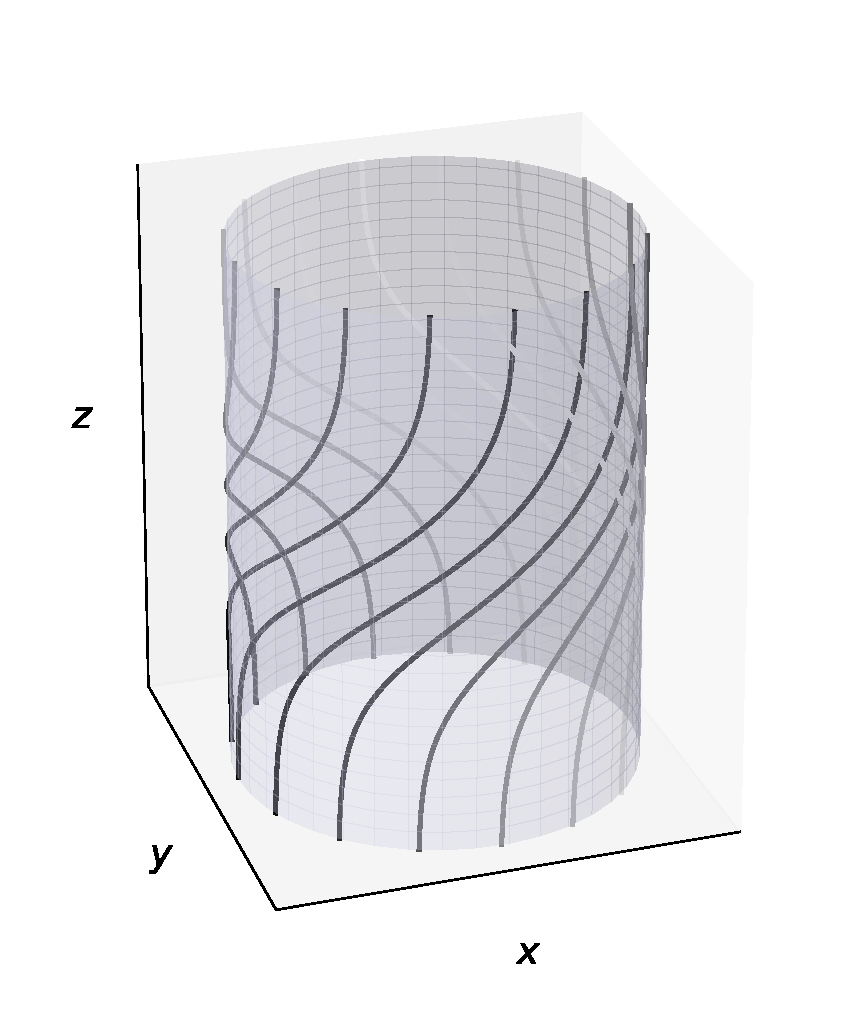
\includegraphics[width=0.5\textwidth]{pics/chap4/field_lines.pdf}
\caption[Magnetic field lines passing through one of the \alfven wave packets]{Magnetic field lines passing through one of the \alfven wave packets (given in Equation~\ref{3dpacket}) used as initial conditions in our 3D simulations.}
\label{field_line}
\end{figure}
%###############################

The packet velocity $\be\times\boldsymbol{B}/B^2$ is set by the initial electric field,
%
\begin{equation}
  \be = \pm \hat{\boldsymbol{z}} \times \bb.
\end{equation}
%
It has opposite signs for the two wave packets.

%###############################
\begin{figure}[h]
\centering
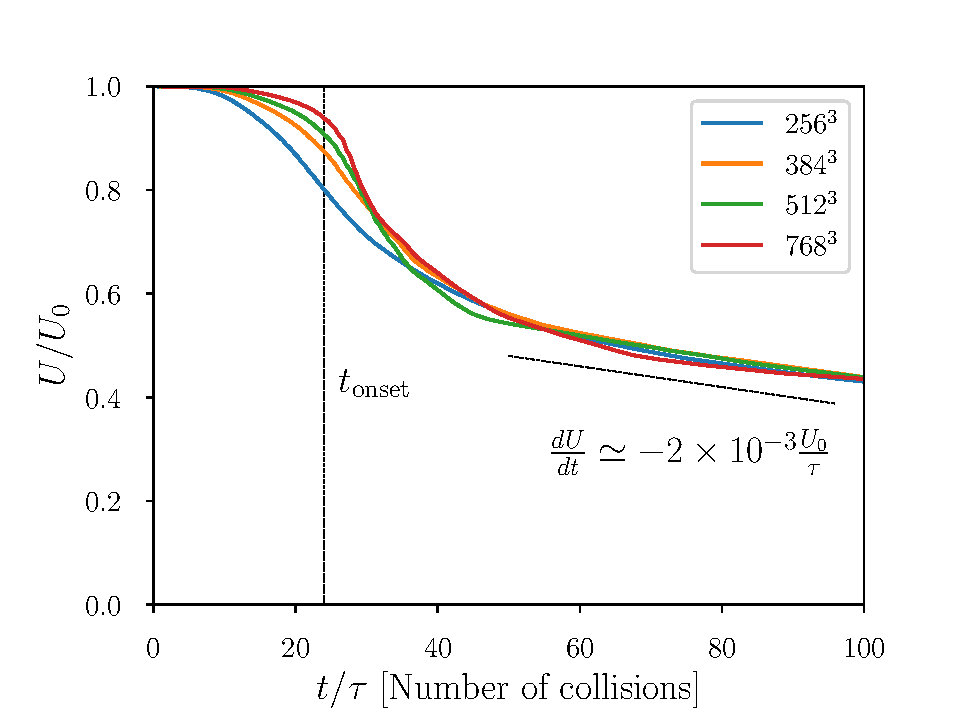
\includegraphics[width=0.6\textwidth]{pics/chap4/convergence3D}
\caption[Free energy evolution for different resolutions in 3D simulations]{Free energy evolution for different resolutions in 3D simulations of colliding \alfven wave packets with amplitude $\xi=0.5$.}
\label{energy3D}
\end{figure}
%###############################

We observe that over time the collisions of the counter-propagating \alfven wave packets lead to the development of a turbulent cascade to small scales. The cascade energy is dissipated primarily by grid-heating (Channel (iv) in Section \ref{dissipation-channels}). 
This interpretation is supported by (1) consistency of the overall energy dissipation rate with increasing grid resolution, (2) observation of a definite time $t_{\rm onset}$ at which energy dissipation commences, and (3) formation of a Kolmogorov-type energy spectrum.

Figure \ref{energy3D} shows the time series of electromagnetic free energy $U(t)$ for the same model, $\xi = 0.5$, at different grid resolutions. 
All of the simulations exhibit an initial phase with slow dissipation lasting $t_{\rm onset}\sim 24 \tau$, a fast dissipation phase between $\sim 24\tau$ and $\sim 40\tau$, and a subsequent gradual relaxation phase. 
The difference between the initial slow and fast dissipation phases becomes more pronounced as the grid resolution increases; the rate of energy dissipation prior to $t_{\rm onset}$ diminishes with increasing numerical resolution. 
Meanwhile, the energy lost by the system at late times $>40\tau$ is independent of the grid resolution to within roughly $5\%$.

\begin{figure}[h]
\centering
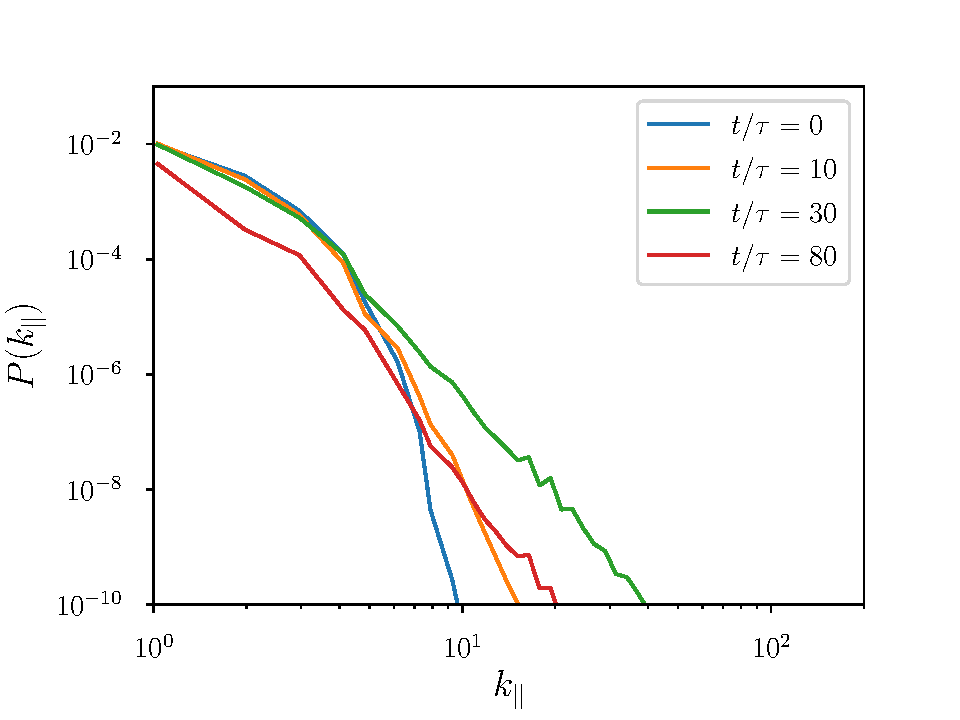
\includegraphics[width=0.48\textwidth]{pics/chap4/spec3Dev_parallel}
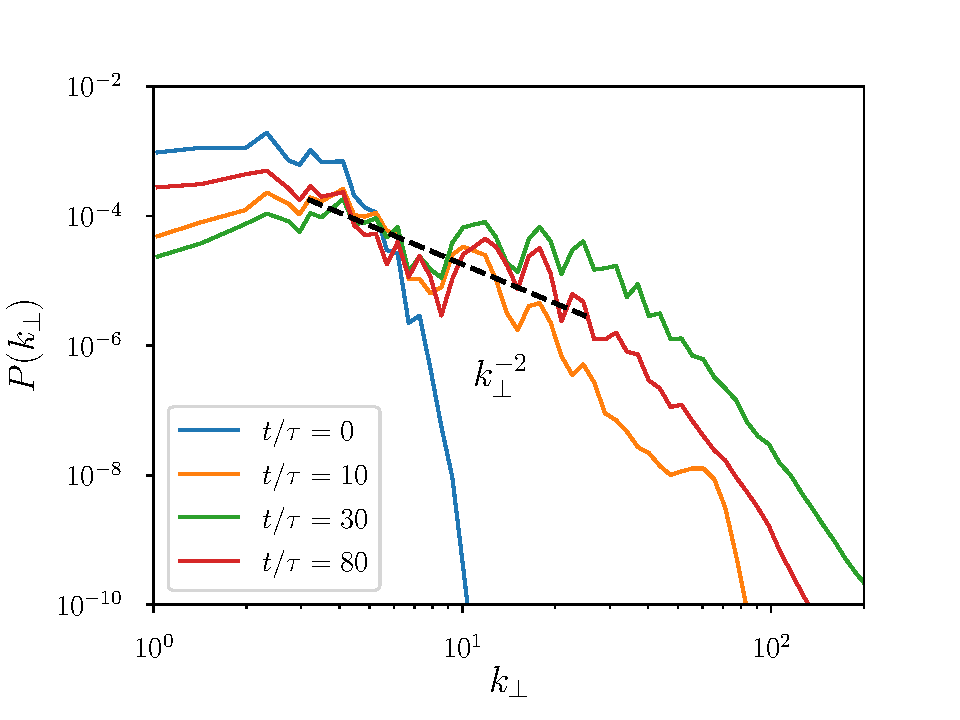
\includegraphics[width=0.48\textwidth]{pics/chap4/spec3Dev}
\caption[Development of turbulent spectrum in 3D simulations]{Development of turbulent spectrum (snapshots at $t/\tau=0$, 10, 30, 80) in the simulation with the initial packet amplitude $\xi=0.5$ and grid resolution $512^3$. Upper panel: spectrum in $k_\parallel$ (parallel to the background field). Lower panel: spectrum in $k_\perp$(perpendicular to the background field).
The dashed line indicates the slope $P(k_\perp)\propto k_\perp^{-2}$.
}
\label{spec3Dev}
\end{figure}
%
Figure \ref{spec3Dev} shows the power spectrum evolution for a simulation with resolution $512^3$. Over time, the system develops waves at progressively increasing wavenumber, indicating a forward energy cascade. The spectrum extends to a maximum wavenumber $k_{\rm max}(t)$, which 
is seen to increase between $t=0$ and $t_{\rm onset}$.
At $t_{\rm onset}$, $k_{\rm max}$ reaches the nominal dissipation wavenumber $k_{\rm diss} \sim N / 10$, where $N$ is the number of grid points in each $(x,y,z)$ direction.
Figure \ref{spec3Dev} also reveals that the spectrum is significantly anisotropic, with $P(k_\perp) > P(k_\parallel)$ at all but the largest scales, indicating that energy cascades primarily in the direction perpendicular to the background field.
Energy cascade in the parallel direction due to the excitation of fast waves is weak compared to that in the perpendicular direction.
As energy moves from large to small (perpendicular) scales, the energy around large $k_\perp$ increases monotonically up until $t_{\rm onset}$, at which time modes around $k_{\rm diss}$ become significantly populated. Subsequently, some energy is reflected back toward low wave numbers, causing the power at large scales to grow between $t_{\rm onset}$ and $80\tau$.
The perpendicular spectrum eventually relaxes to a power-law consistent with $k_\perp^{-2}$ at $\sim 80\tau$. Such spectral slope is consistent with the so-called weak MHD wave turbulence spectrum, as reported by \cite{2001JETP...93.1052K}.

\begin{figure} [h]
\centering
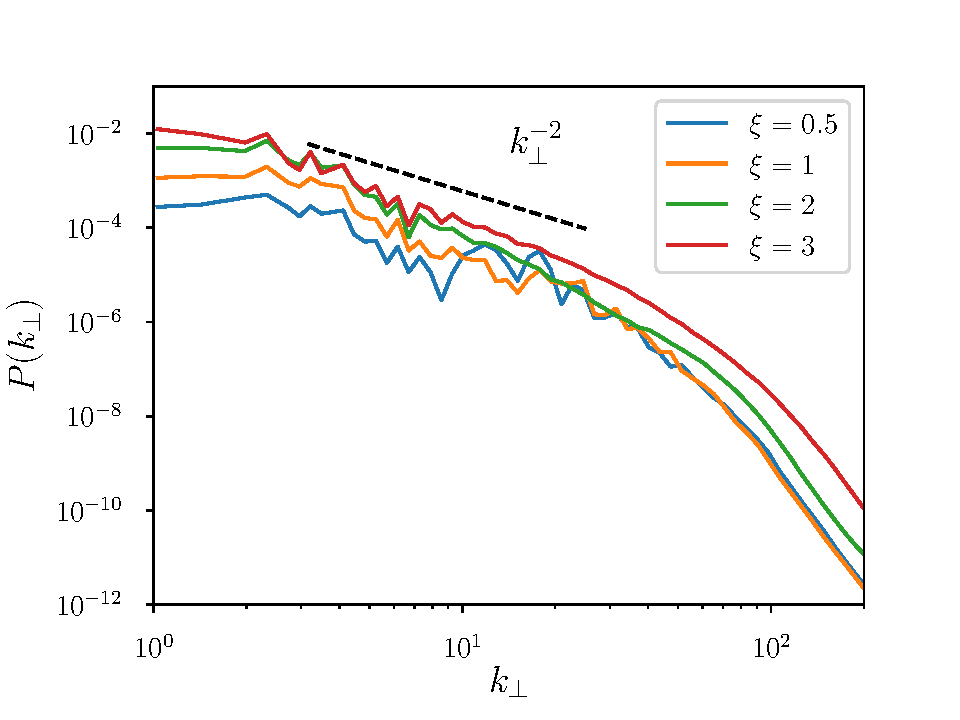
\includegraphics[width=0.6\textwidth]{pics/chap4/spec3Dst}
\caption[Turbulence spectrum in $k_\perp$ in four 3D simulations]{
Turbulence spectrum in $k_\perp$ at $t=80\tau$ in four simulations with different initial packet amplitudes $\xi$.
}
\label{spec3Dst}
\end{figure}

The perpendicular power spectrum exhibits oscillations in $k_\perp$ at times earlier than $80\tau$.
This is due to a known feature of wave turbulence \citep{2011LNP...825.....N}, that energy is transferred mainly through resonant interactions; only a discrete set of secondary modes are excited by the primary modes. The resonant secondary modes then couple with the primaries and further drive the same secondaries. This leads to disproportionate energy transfer between particular sectors of the $k$-space, enhancing the energy concentration around preferred wavenumbers.
Figure \ref{spec3Dst} shows the perpendicular power spectrum after 80 collisions for various amplitudes $\xi$ of the initial wave packets in the range $0.5 - 3$.
The slopes of the perpendicular spectra are all close to $k_\perp^{-2}$.
We observe that the spectral oscillations are weaker for larger values of $\xi$.
This is because the strength of nonlinear interactions increases with $\xi$ and energy is distributed across a larger number of modes within a given time.

The existence of a universal time $t_{\rm onset}$ at which dissipation commences is consistent with a forward energy cascade, and a spectral energy distribution having finite \textit{energy capacity}, meaning that
%
\begin{equation}
	\lim \limits_{k_{\rm max} \rightarrow \infty} \int \limits_{k_0}^{k_{\rm max}} P(k) dk < \infty \, .
\end{equation}
%
This is the case for any power-law spectra $P(k)$ steeper than $k^{-1}$.
Such spectra have the property that the energy stored at wavenumbers higher than $k$ asymptotes toward zero with increasing $k$.
As energy cascades toward smaller scales, $k_{\rm max}$ must either increase without bound (thus exciting modes at the dissipation scale, however small), or some of the energy must be reflected toward larger scales.
We do see evidence in Figure \ref{spec3Dev} for such energy reflection, as the power around $k_\perp \sim 4$ first drops, but then rises again at $t \sim t_{\rm onset}$.
However, the energy distribution subsequently equilibrates to a Kolomogorov spectrum, with energy transferring continuously into the dissipation range, and leading to the divergence of $k_{\rm max}$.
The rapid increase of $k_{\rm max}$ implies that $t_{\rm onset}$ becomes insensitive to $k_{\rm diss}$, and thus to the grid resolution.
Therefore the energy spectrum $P(k_\perp) \propto k_\perp^{-2}$ seen in 3D simulations is compatible with the time series in Figure \ref{energy3D} which suggests a universal value of $t_{\rm onset}$.
In the next section we will show that 2D settings exemplify the opposite behavior, where the spectrum is very shallow, having infinite energy capacity.
Those 2D systems will not display numerical consistency of the dissipation onset time.


\subsection{2D simulations}
%
In our 2D simulations, the field is independent of the $y$ coordinate.
We utilize initial conditions
%
$\bb = B_0\hat{\boldsymbol{z}}+ B_y\hat{\boldsymbol{y}}$ in the $x-z$ plane, where two \alfven wave packets have Gaussian profiles,
%
\begin{equation}
\label{eqn:2d-wave-packets}
	B_y =B_0 \xi \sum\limits_{i=1,2} \exp\left(- \frac{|\boldsymbol{r}-\boldsymbol{r}_i|^2}{\ell^2} \right) \, .
\end{equation}
%
Here, $\boldsymbol{r}_1 = (0,-0.25)$ and $\boldsymbol{r}_2 = (0,0.25)$ are the center positions of the two wave packets in the $x-z$ plane.
The width of the wave packet is the same ($\ell=0.1$) as in our 3D simulations.
The electric field is again $\be = \pm \hat{\boldsymbol{z}}\times \bb$, with opposite sign for each wave packet. The wave packets travel toward one another along the guide field (in the $\pm \hat{\boldsymbol{z}}$ directions), and have a cylindrical envelope in which the magnetic field is perturbed along the cylinder axis $\hat {\boldsymbol{y}}$. 
%
\begin{figure}[h]
\centering
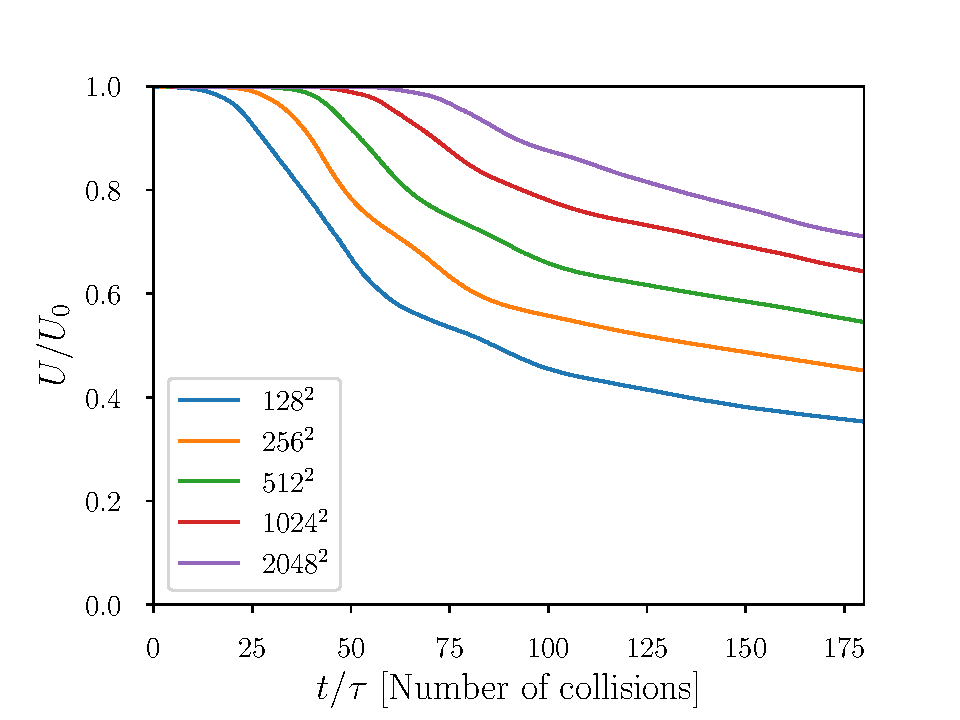
\includegraphics[width=0.6\textwidth]{pics/chap4/convergence2D}
\caption[Free energy evolution for different resolutions in the 2D model]{ Free energy evolution for different resolutions in the 2D model with packet amplitude $\xi=0.4$.}
\label{energy2D}
\end{figure}
%


In 2D simulations, we observe that collisions between counter-propagating wave packets also result in a forward energy cascade.
However, unlike in the 3D case, 2D systems do not exhibit consistency of the overall dissipation rate for different grid resolutions. 
Figure \ref{energy2D} shows the time series of electromagnetic free energy for amplitude $\xi = 0.4$, with different numerical resolution.
The amount of energy $\Delta U$ dissipated before a given time $t_0$ is a decreasing function of the grid resolution, showing no trend toward a universal value.
Moreover, the onset of dissipation occurs at later times; there is no asymptotic $t_{\rm onset}$ that was observed in Section \ref{sec:3d} for the 3D case.
%
\begin{figure}[h]
\centering
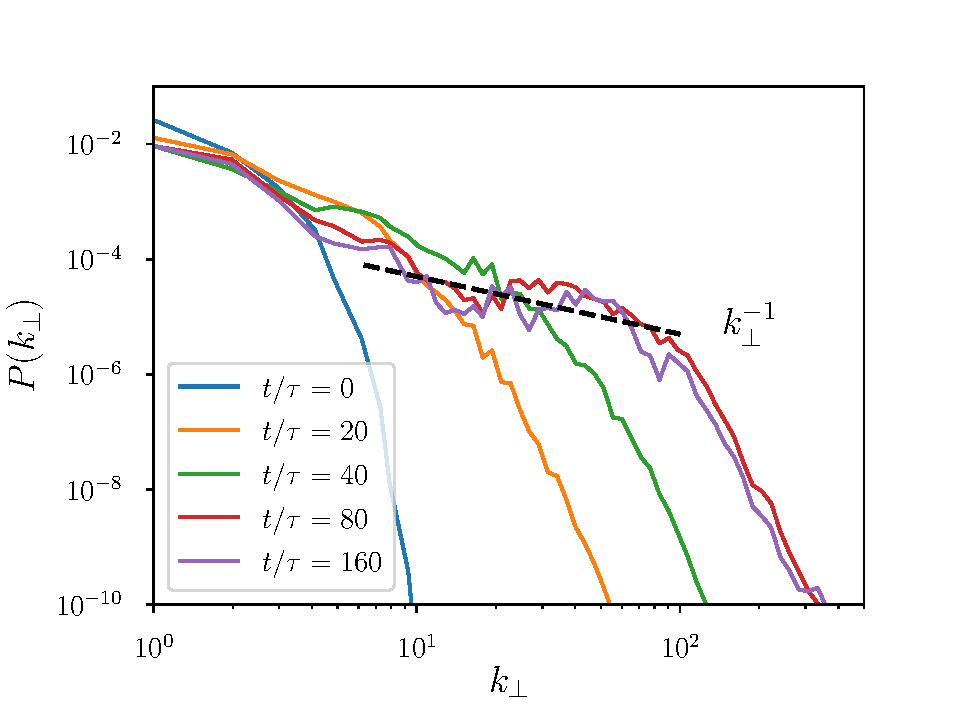
\includegraphics[width=0.6\textwidth]{pics/chap4/spec2Dev}
\caption[Spectrum evolution for the 2D simulation]{Spectrum evolution for the 2D simulation with $2048^2$ resolution and amplitude $\xi =0.4$. The dashed line indicates the slope $P(k_\perp)\propto k_\perp^{-1}$.}
\label{spec2Dev}
\end{figure}
%

The energy spectrum in 2D simulations is also different from the 3D case. Figure \ref{spec2Dev} shows the spectral evolution for a model with $\xi = 0.4$ and grid resolution of $2048^2$. Over the course of tens of collisions, energy is gradually redistributed toward smaller scales, with a perpendicular spectrum $P(k_\perp) \propto k_\perp^{-1}$, significantly shallower than the 3D case.

The different energy dissipation rates seen in 2D versus 3D settings can be explained by the difference in their spectral slopes.
In particular, the energy spectrum in 2D has an unbounded energy capacity, because
%
\begin{equation}\label{eqn:energy-cap}
	U_0 = \alpha \int\limits_{k_{0}} ^{k_{\rm max}} \md k_{\perp} \; k_\perp^{-1} = \alpha 
    \,\ln
    \frac{k_{\rm max}}{k_0}
\end{equation}
%
would diverge if $k_{\rm max}\rightarrow \infty$. Here $\alpha$ is a normalization factor which may evolve with time. As energy cascades toward smaller scales, $k_{\rm max}$ increases, but remains finite. This fact is consistent with the increasing delay of the dissipation onset with increasing resolution, as it takes longer for $k_{\max}$ to reach $k_{\rm diss}$.

The evolution of the $k_\perp^{-1}$ turbulence spectrum is determined by the evolution of its normalization $\alpha(t)$.
Suppose that $k_{\rm max}$ increases as a power law with time, 
%
\begin{equation}
  k_{\rm max} \propto t^q, \qquad q>0.
\end{equation}
%
The normalization $\alpha$ must decrease as $k_{\rm max}$ increases,
%
\begin{equation}\label{eqn:alpha-of-t}
	\alpha(t) = \frac{U_0}{\ln(k_{\rm max}/k_0)} = \frac{U_0}{q\ln t+\beta},
\end{equation}
%
where $\beta$ is a constant. When $k_{\rm max}$ reaches $k_{\rm diss}$, grid heating begins to remove energy on scales smaller than $k_{\rm diss}^{-1}$, and the turbulence energy $U$ decreases below $U_0$,
%
\begin{equation}\label{eqn:U-of-t}
	U(t) = \alpha(t) \int\limits_{k_{0}} ^{k_{\rm diss}} \md k_{\perp}\; k_\perp^{-1} = \alpha(t) \ln \frac{k_{\rm diss}}{k_0}\, .
\end{equation} 
%
Equations \ref{eqn:alpha-of-t} and \ref{eqn:U-of-t} together yield the relation
\begin{equation}\label{eqn:U-model}
	\frac{U_0}{U(t)} = \frac{q\ln t + \beta}{\ln(k_{\rm diss} / k_0)}.
\end{equation}
%
This description assumes that $\alpha(t)$ (or the value of $q$) is independent of grid dissipation at high $k_\perp$. The value of $k_{\rm diss}$ is proportional to the grid resolution $N$ and the evolution of $U$ depends on $N$.

The predicted relation~(\ref{eqn:U-model}) can be tested by measuring $U(t)$ in the simulations with different resolutions and checking (1) whether $U_0/U(t)$ is indeed a linear function of $\ln t$, and (2) whether $q$ indeed has a universal value. This test is shown in Figure~6 for five different resolutions $N$ that span a factor of $16$. In each case, after $k_{\max}$ reaches $k_{\rm diss}$ we observe a linear growth of $U_0/U(t)$ with $\ln t$. We have measured its slope $s$ as a function of $\ln k_{\rm diss}$ and then calculated $q$ from the linear realtion inferred from Equation~(\ref{eqn:U-model}),
%
\begin{equation}
   \frac{1}{s}=\frac{1}{q}\ln\frac{k_{\rm diss}}{k_0}.
\end{equation}
%
For all five resolutions, the values of $(\ln k_{\rm diss},\,1/s)$ are found to follow the same line with $q\approx 1.75$, confirming the above analytical picture of the turbulence spectrum evolution. In contrast to the 3D simulations, dissipation slows down with increasing $N$.

\begin{figure}[h]
\centering
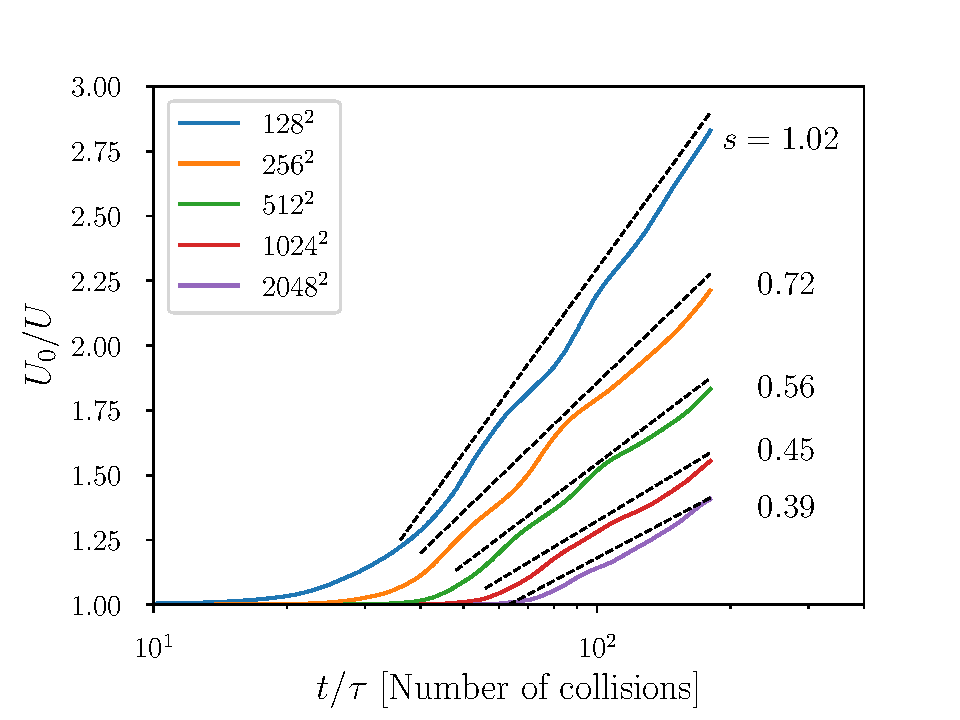
\includegraphics[width=0.6\textwidth]{pics/chap4/model2D}
\caption[The evolution of $U_0/U(t)$ in 2D simulations]{ 
The evolution of $U_0/U(t)$ in 2D simulations. Dashed lines show the best-fit slopes of the linear relation between $U_0/U$ and $\ln t$. The slope value $s$ is indicated next to each curve.}
\label{fit}
\end{figure}

\section{Local dissipation and escape of waves}
\label{sec:fate}

As discussed in Section \ref{sec:ffe}, nonlinear interactions between \alfven waves can excite fast modes. These modes are not ducted along the magnetic field lines; they have group velocity in any direction and may escape the magnetosphere. 
In this section we examine the competition between the two energy sinks: local dissipation of the turbulent cascade and the escape of generated fast waves. 
We use the 3D setup of colliding \alfven wave packets as described in Section~3, and compare two sets of simulations, with and without wave escape, as explained below.
%
\subsection{Turbulent dissipation rate without wave escape}
%
\begin{figure*}
\centering
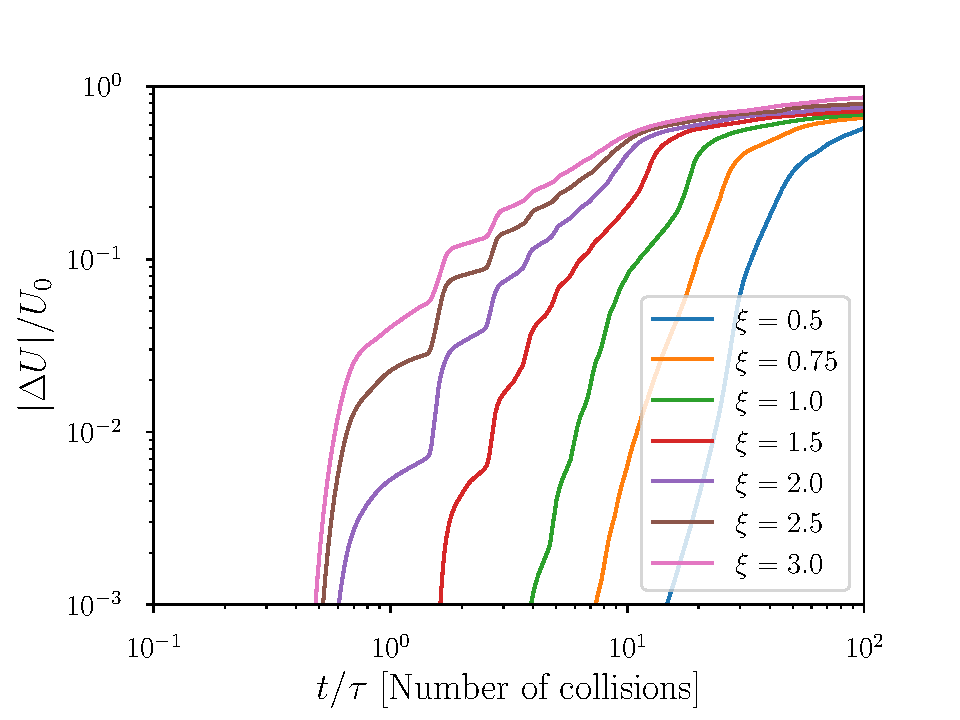
\includegraphics[width=0.48\textwidth]{pics/chap4/casrate3D}
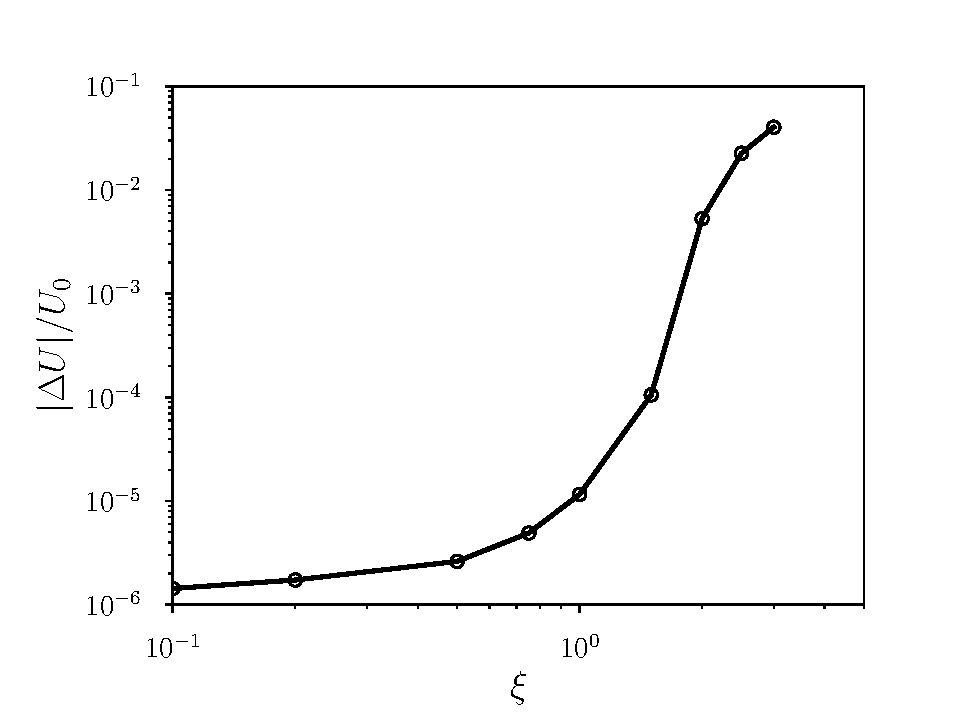
\includegraphics[width=0.48\textwidth]{pics/chap4/dis_col}
\caption[Dissipation of \alfven wave packet energy $U_0$ in 3D simulations]{Dissipation of \alfven wave packet energy $U_0$ in 3D simulations.
\textit{Left} -- Time series for the dissipated $f(t)=|\Delta U|/U_0$. Different curves show models with different packet amplitudes $\xi$.
\textit{Right} -- Dissipated energy fraction $|\Delta U|/U_0$ after the first collision as a function of packet amplitude $\xi$.
}
\label{casraterate3D}
\end{figure*}
%
The periodic boundary conditions for all ($x,y,z$) directions imply that waves cannot escape the computational box; they can only dissipate. The dissipation efficiency depends on the amplitude of the colliding \alfven packets $\xi$. We have studied this dependence by calculating models with seven different values of $\xi$ between 0.5 and $3$, at fixed resolution of $512^3$. The results are presented in Figure~ 7, which shows evolution of the dissipated energy fraction,
\begin{equation}
  f(t)=\frac{U_0-U(t)}{U_0}.
\end{equation}
One can see that $f(t)$ is small in the first collisions, and its time dependence is step-like, because dissipation occurs only during the collisions,
when the two packets overlap. (The  duration of overlap is significantly shorter than the time between the collisions, because the packet width $\ell$ is smaller than the computational box size.) At later times, the field line bundle carrying the two packets becomes increasingly filled with strong \alfven turbulence, capable of dissipating energy outside the packets; then the dissipation curve $f(t)$ becomes smoother.

As expected, $f(t)$ is higher for the simulations with larger packet amplitudes $\xi$, because of the higher effectiveness of the nonlinear interaction.
The dissipated fraction after the first collision, $f_1=f(\tau)$, is plotted in the right panel of Figure \ref{casraterate3D} for different values of $\xi$. 
We find that $f_1$ is a very sensitive function of $\xi$, rising sharply from $10^{-5}$ at $\xi = 1$ to $10^{-2}$ at $\xi = 2$. 

%
\subsection{Turbulent cascade with escaping fast modes}
%
To evaluate the energy radiated away by fast modes, we have introduced a ``sponge'' layer along the transverse domain boundaries, intended to absorb fast waves reaching the boundaries.
The elimination of energy transported by fast waves into the sponge layer simulates their escape.

The sponge layer is implemented by adding an Ohmic-like dissipation term $-\sigma_s \be$ to the force-free current in Equation \ref{current}. This term leads to exponential damping of the electric field on the timescale $\sigma_s^{-1}$. 
We adopt a spatial profile of $\sigma_s(x,y)$ that leads to faster damping of the electric field near the boundary of the computational domain in $x$-$y$ plane ($0<x<1$; $0<y<1$),
%
\begin{equation}
	\sigma_s = \frac{1}{2 \tau} \left( 1 - e^{-8 \delta^4} \right), \qquad  \delta = \max \left(\frac{\varpi - r_0}{d - r_0}, 0 \right),
\end{equation}
%
where $\varpi = \sqrt{x^2+y^2}$, $d = 0.5$ is half of the transverse domain scale, and $r_0 = 0.3$ is the distance from the $z$-axis within which absorption is switched off completely, $\sigma_s=0$.
Near the boundary, the damping time scale $\sigma_s^{-1}$ drops to $2 \tau$ (equal to the light crossing time of the computational box).
The energy dissipated in the sponge layer is a proxy for energy escaping the system in the form of fast waves.

The loss of fast modes at the boundaries leads to a faster decline of the free energy in the box $U(t)$ compared with the simulations without wave escape.
The magnitude of this effect is a measure of the effectiveness of the energy loss through the boundaries compared with local dissipation through the turbulent cascade.
Figure \ref{3Dfastwave} shows the comparison of four pairs of simulations with and without the sponge layer (identical otherwise). All eight simulations have resolution $512^3$. The four different amplitudes $\xi=0.5, 1, 2, 3$ are chosen to investigate how the competition between wave escape and turbulent damping depends on the initial amplitudes of the packets.

For instance, in the simulation with $\xi = 0.5$, during the first $10$ collisions (prior to $t_{\rm onset}$), fast waves carry away $\sim 2\%$ of the initially available free energy $U_0$, compared to $\sim 1\%$ taken by turbulent dissipation.
Radiation of fast waves is thus the primary energy loss channel prior to the onset of developed turbulence. After turbulence is fully developed, at times $\gtrsim t/\tau=100$, 
the energy radiated by fast waves accounts for only $6\%$ of $U_0$ while turbulent dissipation accounts for nearly $60\%$.

A smaller energy fraction is carried away by fast waves in the simulations with larger $\xi$.
In the run with $\xi=3$, the sponge layer accounts for only $3\%$ of $U_0$.
This trend is the result of a stronger coupling of fast waves in nonlinear interactions.
As the fast waves participate in the turbulence to a greater degree, they are scattered and damped more efficiently, dissipating more energy locally in the magnetosphere.
%
\begin{figure}[h]
\centering
\includegraphics[width=0.6\textwidth]{pics/chap4/casrate3Dohm}
\caption[Comparison between free energy evolution $U(t)$ in the simulations with and without damping of fast modes]{Comparison between free energy evolution $U(t)$ in the simulations with (dashed curves) and without (solid curves) damping of fast modes at the boundary. 
The difference between solid and dashed curves shows the effect of fast mode escape compared with local dissipation through the turbulent cascade.
}
\label{3Dfastwave}
\end{figure}
%

\section{Enhanced immediate dissipation and FFE failure}
\label{sec:breakffe}
%

The results of the preceding sections show that wave damping takes many crossing times $\tau$, even at very high amplitudes $\xi>1$. Since this conclusion is based on numerical simulations with a concrete setup, one would like to know whether the conclusion is robust. To address this question we have tried to vary the initial setup of the \alfven wave packets in search for more efficient damping, and found that in some cases (both 2D and 3D) our FFE simulations predict much quicker dissipation, which occurs immediately in the first collisions of the wave packets, even before the development of turbulence.

\subsection{Immediate dissipation observed in FFE simulations}
The immediate dissipation effect is sensitive to the initial polarization of the wave packets. It is maximized (and most convenient to study) in the simplest 1D ``slab'' setup. Then the initial perturbations of the magnetic field in the two colliding packets, $\bb_1$ and $\bb_2$, can point in any two chosen directions in the $x$-$y$ plane perpendicular to the guide field $\bb_0$. The angle between $\bb_1$ and $\bb_2$ will be denoted by $\theta$. The relative polarization $\theta$ is an important parameter of the packet collision problem, in addition to the packet amplitude $\xi$.

The simple 1D setup is better suited for the study of polarization effects than the 3D and 2D setups of the preceding sections. Recall that in the 3D setting the spherical packets could not have a single direction for $\bb_1$ or $\bb_2$, and thus the polarization angle was not well defined. In the 2D setting explored in Section~4.2, we chose $\bb_1$ and $\bb_2$ along the $y$-axis perpendicular to the simulation plane $x$-$z$, which allowed us to confine the packets in a circular region in the $x$-$z$ plane. However, the requirement of $\bb_{1,2}$ being parallel (or anti-parallel) to the $y$-axis leaves only two possibilities for the relative polarization, $\theta=0$ or $180^\circ$, and in Section~4.2, we stuck to the case of $\theta = 0^\circ$.
Therefore, in both 3D and 2D simulations presented in Section~4 we observed dissipation only through turbulence cascade to the grid scale, which takes a significant time.

The reason for immediate damping discussed in the present section is the activation of the dissipation channel (iii) listed in Section~3.5. Our FFE simulations show, for some values of $\theta$ and $\xi$, field evolution that violates the condition $E<B$, and then the procedure of enforcing this condition (Section~3.4) creates strong dissipation.

One can see the role of relative polarization $\theta$ for this effect from a simplified consideration that neglects the nonlinear character of  packet collisions and merely looks at the linear superposition of the colliding packets. When $\bb_1$ and $\bb_2$ are parallel ($\theta=0$), the magnetic fields of the packets add constructively while their electric fields add destructively --- the opposite Poynting fluxes of the two packets $\be_1\times \bb_1$ and $\be_2\times\bb_2$ require them to have antiparallel electric fields $\be_1$ and $\be_2$. 
By contrast, when the packets have nearly anti-aligned $\bb_1$ and $\bb_2$, the electric fields $\be_1$ and $\be_2$ become parallel and add constructively making it possible for $E$ to exceed $B$ for sufficiently large amplitudes $\xi$.

A simple estimate gives the range of $\theta$ and $\xi$ where this effect may be expected.  Let us consider two counter-propagating packets of amplitude $\xi$ centered at $z_1(t)$ and $z_2(t)$. The packets can have, for example, a Gaussian shape, $B_{1,2}=\xi B_0\exp[-(z-z_{1,2})^2/\ell^2]$. Let us choose the $y$-axis along $\bb_1$; then
%
\begin{eqnarray}
   \bb_1&=&\xi \exp\left[-\frac{(z-z_1)^2}{\ell^2}\right]\,\boldsymbol{b}_1, \quad 
       \boldsymbol{b}_1=(0,1,0) \\
   \bb_2&=&\xi \exp\left[-\frac{(z-z_2)^2}{\ell^2}\right]\,\boldsymbol{b}_2, \quad 
       \boldsymbol{b}_2=(\sin\theta,\cos\theta,0).
\end{eqnarray}
%
where we use the units $B_0=1$, . The corresponding electric fields are $\be_{1,2}=\mp \hat{\boldsymbol{z}} \times \bb$,
so the angle between the electric fields is $180^\circ - \theta$.
%
If the non-linear interaction of the packets is neglected, then at the point of maximum overlap (at $z=z_1=z_2$) the superposed field magnitudes would be
%
\begin{eqnarray}
	(\bb_1+\bb_2)^2 &=& 2\xi^2(1+\cos\theta) + 1 \\ \nonumber
	(\be_1+\be_2)^2 &=& 2\xi^2(1-\cos\theta) \, .
\end{eqnarray}
%
Magnetic dominance would thus be lost when
%
\begin{equation}\label{cr1}
	-4\xi^2\cos\theta >1 \, .
\end{equation}
%
% which 
This condition can be satisfied if $\theta>90^\circ$, and is easiest to satisfy if $\theta=180^{\circ}$. In the latter case, a moderately strong amplitude $\xi>0.5$ is required.
%
\begin{figure}[h]
\centering
\includegraphics[width=0.6\textwidth]{pics/chap4/dis1D}
\caption[Dissipated energy fraction in the 1D wave packet collision as a function of the relative polarization angle $\theta$]{Dissipated energy fraction in the 1D wave packet collision as a function of the relative polarization angle $\theta$, for various amplitudes $\xi$ of the colliding packets.}
\label{dis1d}
\end{figure}
%
%%%%%%%%%%%%%%%%%%%
\begin{figure}[h]
\centering
\includegraphics[width=0.6\textwidth]{pics/chap4/alfven180_deltaB08_single_collision.pdf}
\caption[Comparison of the FFE simulation with the full MHD simulation]{
Comparison of the FFE simulation (dashed curve) with the full MHD simulation that tracks both plasma energy and electromagnetic energy (solid curves). The colliding \alfven wave packets have amplitude $\xi=0.8$ and relative polarization angle $\theta = 180^\circ$. Numerical convergence of the MHD simulation is shown by plotting the results obtained with resolutions $N=256,512,1024,2048$ (the increasing line thickness corresponds to the increasing resolution).
}
\label{rmhd}
\end{figure}
%%%%%%%%%%%%%%%%%%%

In general, such large amplitude waves interact non-linearly and their magnitude cannot be determined by linear superposition. Remarkably however, we observe from Equation \ref{current} that in FFE the non-linear terms vanish for 1D anti-polarized plane waves counter-propagating along $\bb$. 
Thus, when $\theta = 180^\circ$, the wave packets pass through one another unchanged, as long as $E<B$, and the linear superposition estimate for the loss of $E<B$ condition should be accurate.

%%%%%%%%%%%%%%%%%%%
\begin{figure*}[h]
\centering
\includegraphics[width=\textwidth]{pics/chap4/snapshots}
\caption[Snapshots of the FFE and MHD simulations]{
Snapshots of the FFE (orange) and MHD (blue) simulations shown in Figure~\ref{dis1D}. 
The snapshots are taken at four times, from $t=0$ (left) to $t=0.5$ (right) in units of the light crossing time of the computational box. 
}
\label{snapshots}
\end{figure*}
%%%%%%%%%%%%%%%%%%%

These expectations are tested in Figure~9, which presents the simulation results for the 1D setup described above. It shows the fraction of energy dissipated after a single collision of the two packets, $f_1=|\Delta U|/U_0$, for different values of the relative polarization angle $\theta$ and packet amplitude $\xi$. We find that strong dissipation, caused by the imposed shortening of the electric field to sustain $E<B$, becomes active for nearly anti-polarized packets if $\xi \gtrsim 0.5$. For example, we see 20\% energy loss after a single collision when $\xi = 0.6$ and $\theta = 180^\circ$. As $\xi$ increases to 1.4, we observe $f_1$ growing to $\sim 90$\% for $\theta$ approaching $180^\circ$, and exceeding 10\% for $\theta>135^\circ$.
 
Figure \ref{dis1d} also reveals a second peak in $f_1(\theta)$ near $\theta=90^\circ$. This peak is not predicted by the above linear superposition estimate, and thus has a nonlinear origin. However, it is also caused by the violation of $E<B$ condition.
It can be understood by looking at the evolution of $\be\cdot \bb$ in the linear superposition approximation, $\be\cdot \bb = 2\xi^2\sin\theta$. 
The linearly superposed fields would violate the FFE condition $\be\cdot \bb=0$, and nonlinear effects are responsible for sustaining this condition: the system is forced to generate a longitudinal electric field $E_z \propto \xi^2$, and for large enough $\xi$ this electric field component leads to the loss of magnetic dominance. 
This effect is proportional to $\sin\theta$ and thus strongest at $\theta\approx 90^\circ$.

\subsection{MHD simulations and the spurious character of immediate dissipation in FFE}
%
One may conclude from the FFE simulations that the collisions of large-amplitude \alfven waves with favorable polarization 
gives strong immediate dissipation. The dissipation mechanism in this case is the result of the customary procedure of shortening $E$ to sustain $E<B$. 
However, we point out that there is no guarantee that this procedure correctly captures the true field evolution. 
The true behavior of the system when $E$ reaches $B$ is outside the realm of FFE and can be understood only with a more complete physical model. The model must explicitly include a component of the system that takes the energy (and momentum) lost by the field.

Therefore, we have performed similar simulations of the 1D packet collisions in the full relativistic MHD, which does not neglect the plasma stress-energy tensor, and conserves the total energy and momentum of field and plasma. Plasma moves with a subliminal velocity $\boldsymbol{v}$, and MHD simulations never break the condition $E<B$, since the electric field $\be = -\bV \times \bb$ is obtained from the primitive variables, rather than evolved independently as it is in FFE. We use the relativistic MHD code \texttt{Mara} \citep{2012ApJ...744...32Z}.

MHD is expected to approach the FFE regime in the limit of high magnetization $\sigma\gg 1$. Therefore, in our simulations we choose a high $\sigma=25$, where $\sigma=B_0^2/\rho_0$ is defined for the background magnetic field $B_0$ and $\rho_0$ is the initial (uniform) plasma density in the computational box. 
Otherwise, the simulation setup is the same as described in Section~6.1 for the 1D FFE simulations.

Figure \ref{rmhd} compares the MHD and FFE results. For this test we chose the case where the colliding packets have amplitude $\xi=0.8$ and are anti-polarized ($\theta=180^\circ$).
We see that MHD and FFE predict similar evolution of the free electromagnetic energy $U(t)$ up through the peak of the collision. 
Then the MHD evolution strongly deviates from the prediction of the FFE simulation.
Importantly, the electromagnetic energy lost in the MHD simulation is compensated by a gain in the plasma kinetic energy, while the FFE code removes that same energy $\Delta U$ from the simulation irreversibly by the $E < B$ fix. 

Note that the electromagnetic fields of the two packets initially carry a significant $y$-momentum of the same sign. The MHD simulation shows that during the collision a large fraction of this momentum is taken by the plasma. The plasma momentum density is enhanced at the interface between the colliding packets by a factor $\sim 20$, comparable to $\sigma$. This enhancement is caused by two factors: the plasma is compressed by a factor of $\sim 6$ and the Lorentz factor of its transverse drift ($\boldsymbol{v}_\perp=\be\times\bb_0\parallel -\hat{\boldsymbol{y}}$) exceeds 3.
As a result, a large fraction of the packet electromagnetic energy temporarily converts into bulk kinetic energy of the plasma accelerated along the $y$-axis.
Once the collision is over, the accelerated plasma is stopped by magnetic stresses, restoring the electromagnetic field energy nearly to its initial value. 

Figure~\ref{snapshots} shows in more detail the evolution of the field and plasma in the FFE and MHD simulations.
Unlike the FFE, the MHD system does not reach the ``floor'' $B^2-E^2=0$, because it would correspond to the drift speed equal to the speed of light and hence infinite kinetic energy of the plasma. The plasma is strongly accelerated when $B^2-E^2$ is reduced, and the subsequent dynamics are completely different in the two simulations.
We conclude that the strong dissipation effect observed in FFE simulations is spurious. It is caused by the failure of FFE simulations to keep track of energy that is temporarily removed from the electromagnetic field when $E$ approaches $B$.

\section{Discussion}\label{sec:discussion}
%

The fate of \alfven waves excited in a magnetar magnetosphere is interesting from observational point of view if the wave energy eventually converts to radiation.  In particular, the hot plasma fireball formed in giant flares could be powered by dissipation of waves \citep{1995MNRAS.275..255T}, or the waves may be absorbed by the neutron star and feed surface afterglow emission \citep{2015ApJ...815...25L}. In the relativistic magnetospheres, where the magnetic field dominates over the plasma rest mass and all waves propagate with the speed of light, the nonlinear behavior of wave turbulence is poorly known. In this paper we employed numerical simulations to systematically study turbulence excited by colliding packets of \alfven waves and the resulting dissipation. The packets are assumed to be launched by an unspecified triggering event (e.g. a fast displacement of the crust or a global magnetospheric instability), which determines the initial packet amplitude $\xi = \delta B / B_0$ and size $\ell$.


\subsection{Summary of results}


Most of our results are obtained from high-resolution FFE simulations in a Cartesian box, using the 5th order conservative finite differencing scheme described in \cite{2011MNRAS.411.2461Y}. 
We have also explored situations where the FFE approximation becomes insufficient; then we employed relativistic MHD simulations. Our results are as follows.

(1) Our 3D simulations of packet collisions show that significant dissipation begins when a turbulence cascade develops down to the grid scale. 
The cascade is dominated by modes with wavevectors orthogonal to the background magnetic field, $k_\perp\gg k_\parallel$, and its
spectrum is steep, with a slope close to $-2$. We observed consistency of the cascade and the resulting dissipation rate with increasing grid resolution, and concluded that dissipation of the 3D turbulence is well modeled by ``grid heating'' (the removal of high-$k$ modes on the grid scale). 
The simulations reveal that even for wave packets of enormous amplitudes $\xi=1-3$ dissipation develops slowly, over many ($10-100$) collisions of the packets bouncing in the magnetosphere. The main reason for the dissipation delay is the relatively slow development of the broad spectrum of high-frequency modes and the onset of a persistent energy flow in the cascade down to the dissipation scale. Note that the simulation results presented are based on the initial condition given in Equation~\ref{3dpacket}, which is symmetric around the $z$ axis. However, we have also performed simulations in which the wave packets were stretched in one of the transverse directions $x$ or $y$. The dissipation rates for collisions between these non-axisymmetric wave packets were not appreciably different.

(2) We have found that it is essential to calculate the wave turbulence in three dimensions. Similar simulations restricted to two dimensions (where the fields are assumed to be independent of one  coordinate running transverse to the guide field $\bb_0$) are deficient. They produce qualitatively different results and show no convergence with increasing resolution, because the 2D cascade has a flat spectrum with an infinite energy capacity.

(3) \alfven waves are trapped, because they are ducted along the magnetic field lines, however their collisions generate fast modes that can carry energy away across the field lines. We have measured energy loss due to fast mode escape and found this effect to be weaker than energy dissipation on the field lines carrying the \alfven waves.

(4) When two strong \alfven waves collide, the electromagnetic field can experience immediate significant energy loss. This effect is qualitatively different from the cascade dissipation on the grid scale. It occurs when the Lorentz invariant $B^2-E^2$ is pushed to zero during the field evolution in some parts of the colliding packets, threatening to violate the condition $E<B$. This effect is possible only for certain relative polarizations of the colliding waves and is maximum when the waves have anti-aligned magnetic fields, as demonstrated by a simple 1D model. Our simulations revealed that $B^2-E^2$ can be pushed to zero also in a collision of waves with orthogonal polarizations; this occurs due to a non-linear effect responsible for sustaining $\be\cdot\bb=0$.

(5) We have shown that the permanent energy loss in FFE simulations caused by $B^2-E^2\rightarrow 0$ is spurious.
FFE has no component of the system other than the electromagnetic field and thus has no choice but to permanently remove the energy lost by the field. Our relativistic MHD simulations revealed that in fact this energy is temporarily stored in the
plasma that is compressed and
accelerated to a high Lorentz factor perpendicular to the background magnetic field $\bb_0$.
As the two colliding wave packets finish their interaction, the relativistic plasma motion is eventually decelerated and most of its energy is returned to the electromagnetic field. 

Our results indicate that damping of \alfven waves in the magnetosphere is surprisingly slow even at extremely high amplitudes, and so the waves can bounce in the magnetosphere for many crossing times. We have discussed the physical reasons for this behavior, and conclude that the slow damping is likely a true feature, not an artifact of our approximations. However, one should bear in mind the following simplifications adopted in our simulations.  
\\
(1) Our computational box was rectangular and filled with a uniform background magnetic field $\bb_0$. Magnetic field lines in a real magnetosphere are curved and can extend far from the star, where the field is much weaker. \alfven waves bouncing on such extended field lines will significantly increase their amplitudes as they propagate in the outer weak-field region.
The dissipation rate might also be different if the background magnetic field were strongly twisted. Such conditions would be relevant if, for example, the cascade were triggered by an instability in a strongly twisted magnetosphere \citep{2013ApJ...774...92P}. Investigation of wave turbulence in inhomogeneous (including current-carrying) background fields will be addressed in a future study.
\\
(2) We focused on magnetospheres with energy density $B^2/8\pi$ much greater than the plasma rest mass. This regime almost always holds for the magnetosphere of 
a neutron star. However, during a giant flare, a significant fraction of the magnetic energy may be dissipated and stored in the electron-positron fireball trapped in the magnetosphere. Then the plasma inertia can become a significant factor in the evolution of \alfven wave turbulence.
\\
(3) Our simulations assumed perfect reflection at the boundaries that represent the stellar surface in the computational box. Since the two colliding packets are symmetric in our simulation setup, their perfect reflection at the surface is equivalent to periodic boundary conditions. In reality, the reflection coefficient is slightly below unity, and $\sim 10$\% of the packet energy is transmitted into the star \citep{2015ApJ...815...25L}. 
The transmitted \alfven waves might trigger a global yielding in the magnetar crust \citep{2017ApJ...841...54T}, and brittle yielding could excite high-frequency oscillations of the magnetospheric field lines, enhancing the cascade rate.
\\
(4) We described the spurious immediate dissipation in packet collisions using only 1D (FFE and MHD) simulations. As one can see from Figure~\ref{snapshots}, a short-lived current sheet forms at the packet collision interface, in the $x$-$y$ plane perpendicular to $\bb_0$. 
Our MHD simulations show that FFE does not correctly capture dissipation, however MHD simulations may still be insufficient, because the ideal MHD condition $E<B$ is broken in the current sheet, causing some dissipation. Further study requires kinetic plasma simulations. It is also possible that the current sheet becomes tearing unstable, and magnetic reconnection occurs.
As a first step, we have run several test (1D and 2D) simulations using kinetic code TRISTAN-MP. 
We found that a short-lived current sheet with $E>B$ does form and can dissipate $\sim 20\%$ of magnetic energy. However, this effect is only important for amplitudes $\xi>1$. We also found that magnetic reconnection becomes important when $\xi\gg 1$. The detailed kinetic simulations of dissipation in packet collisions are left to a future paper.

\subsection{Fate of wave energy in magnetar flares}

One implication of our results is that dissipation of \alfven waves in the magnetosphere is less efficient than their absorption by the neutron star. \citet{2015ApJ...815...25L} showed that $\sim 10$ interactions of the wave packet with the stellar crust is sufficient to absorb a large fraction of its energy. That work simulated \alfven wave packets hitting the neutron star crust with realistic density profile $\rho(z)$ and obtained the reflection and transmission coefficients for this interaction, $\mathcal{R}$ and $\mathcal{T}$. The numerical results were also found consistent with an analytical estimate for wave tunneling into the crust using WKB approximation. For typical magnetar fields $B_0>10^{14}$~G  and sizes of the wave packet $\ell\sim 10$~km (comparable to the star radius), the transmission coefficient is $\mathcal{T}=10-20\%$. It increases for stronger $B_0$, because it implies a higher \alfven speed inside the magnetar crust.

The shear wave transmitted into the heavy crust is much slower than the magnetospheric \alfven wave. It continues to propagate into the deeper and denser crustal layers with a decreasing speed and a diminishing amplitude. 
However the strain in the wave {\it grows} as $\propto \rho^{1/4}$ and eventually induces a plastic flow. As a result, the wave energy converts to heat, melting the solid material at the bottom of the liquid ocean, which is $\sim 100$~m deep in magnetars. Thus, most of the magnetospheric wave energy is expected to convert to heat at $\sim 100$~m below the stellar surface. \citet{2015ApJ...815...25L} also calculated how the heat diffuses from this depth and is mostly lost to neutrino emission; a fraction $\sim 0.1$ of the heat will reach the surface and feed the surface afterglow weeks to months after the event that triggered the magnetospheric waves.

Only a fraction $\fdiss$ of  the magnetospheric wave energy will be dissipated locally in the magnetosphere (and an even smaller fraction $\fesc$ will convert to fast modes that escape the field lines carrying the \alfven waves). In particular, in our simulations, the wave energy fraction dissipated per collision of packets is $ \lesssim 1\%$, which is $\gtrsim 10$ times lower than $\mathcal{T}$. Therefore, we roughly estimate $\fdiss\lesssim 0.1$. It may still be interesting for powering fireball radiation. However, a more promising source for fireball energy appears to be magnetic reconnection in a global instability of the over-twisted magnetosphere, as observed in the simulations of Parfrey et al. (2013). The reconnection event immediately dissipates significant energy. It also launches strong waves, which dissipate with efficiency $\fdiss$ in the magnetosphere, but mostly disappear into the star and feed its invisible neutrino emission and a delayed afterglow from the stellar surface.

% Local Variables:
% TeX-master: "../thesis"
% zotero-collection: #("16" 0 2 (name "Thesis"))
% End:
\zotelo{../thesis.bib}

\chapter{Conclusions}
\label{chap:conclusions}

In this dissertation, we explore several topics regarding the magnetodynamics inside and outside magnetars. 
We focus on the dynamics of magnetic fields coupled with the mechanical response of the magnetar, especially the plastic deformation of the crustal materials. 
In the magnetar crust, we have shown that the Hall evolution of strong magnetic fields can accumulate magnetic stress which will trigger plastic failures.
Motion of magnetic footpoints on the magnetar surface is induced as a result of plastic crustal deformations which twists the magnetosphere.
Subsequent X-ray emission from the untwisting of the twisted magnetosphere are demonstrated to be consistent with observations of magnetar outbursts in our 1D simulations.
The reverse process of magnetic energy released in the magnetosphere to be transported into the crust can also occur, especially when the energy is carried by \alfven waves during giant flares.
We have calculated the transmission coefficient of \alfven waves into the crust is of order $\sim 10\%$.
The transmitted waves are compressed in the crust with their strain increased.
Eventually, plastic failures are triggered by the waves and dissipate the magnetic energy to heat in the crust.
The heated crust loses the major fraction of heat through neutrino emission while a small fraction is conducted to the surface and powers a thermal afterglow.
The process of crustal dissipation of \alfven waves competes with the magnetospheric dissipation through the turbulent cascade.
We have performed numerical simulations in the setting of force-free electrodynamics to study the turbulent dissipation process.
Our results suggest that the turbulent dissipation is slow compared to the crustal dissipation unless the waves have amplitude much larger than the background field.
Conversion of \alfven pairs to fast waves which can escape the magnetosphere provides another channel of wave energy loss.
This process is also present in our simulations and is also found to be slow.
The breakdown of force-free conditions $E<B$ and $\be\cdot\bb=0$ is thought to be an efficient dissipation channel of magnetic energy.
In our simulations, this process is observed for \alfven waves with anti-aligned magnetic field.
However, through comparison with relativisitic MHD simulations, we found that energy dissipation is overestimated in FFE simulations and requires further study using kinetic simulations.

The dynamics of strong magnetic fields have profound implications for the high energy radiation from the magnetars.
In this thesis, the interaction of magnetic fields and the magnetar crust is proposed to produce magnetar outbursts as well as delayed afterglow of giant flares.
But this thesis is far from a complete study of the effects of strong magnetic fields in the crust or in the magnetosphere.
The outburst model from crustal failures occurs on the timescale much longer than a millisecond.
How magnetic energy can be quickly released into the magnetosphere on the millisecond scale necessary to explain the short rise time of magnetar bursts and giant flares is still not clear.
Magnetic reconnection as a fast dissipation mechanism of magnetic energy is not studied in this dissertation.
Whether magnetic reconnection can be triggered in 3D simulations and explain magnetar bursts and giant flares remains to be explored.
The high surface temperature of magnetars poses another unanswered theoretical question for the heating and cooling of magnetars.
In addition, the heating of magnetar crust from plastic deformations can thermally unpin the superfluid vortices and the redistribution of vortices can lead to interesting timing anomalies \citep{1996ApJ...457..844L}.

New high energy astrophysical phenomena and future observational missions also require better knowledge of the dynamics of strong magnetic fields.
Magnetic instabilities and dynamos are observed in simulations of binary neutron star mergers to amplify the magnetic fields to $10^{16-17}$~G \citep{2014PhRvD..90d1502K,2015ApJ...809...39G}.
High energy radiation from the strong magnetic fields might serve as another electromagnetic counterpart of binary neutron star merger events.
Fast radio bursts (FRB) are another contemporary mystery of theoretical high energy astrophysics, and magnetars are the central source in many theoretical proposals \citep{2017MNRAS.468.2726K,2018ApJ...868L...4M,2019MNRAS.485.4091M}.
The physics of the strong magnetic fields is essential to connect existing FRB models with observations in order to prove or falsify them.
Future X-ray observations, especially IXPE \citep{WEISSKOPF20161179} and eXTP \citep{2016SPIE.9905E..1QZ}, are proposed to measure the polarization of X-ray emissions which can probe the magnetic field structure of magnetars and possibly QED effects in the ultra-strong magnetic fields.
The study of the magnetodynamics inside and outside magnetars remains interesting and exciting in the future.





% Local Variables:
% TeX-master: "../thesis"
% zotero-collection: #("16" 0 2 (name "Thesis"))
% End:


%%%%%%%%%%%%%%%%%%%%%%%%%%%% Reference %%%%%%%%%%%%%%%%%%%%%%%%%%%%%%
\bibliographystyle{apj}
\pagestyle{myheadings}
\markright{}
\bibliography{thesis}

%%%%%%%%%%%%%%%%%%%%%%%%%%%% Appendix %%%%%%%%%%%%%%%%%%%%%%%%%%%%%%
\begin{appendices}
  \zotelo{../thesis.bib}
\newcommand{\abs}[1]{\left|{ #1}\right |}

\chapter{Wave Turbulence}
\label{app:wave-turbulence}
In the problem of wave turbulence, we are interested in the statistical properties of an ensemble of waves which interact nonlinearly.
For a real wave $\psi(x,t)$ in a $d$-dimensional box of length $L$ with periodic boundary condition, its Fourier coefficient of $\psi$ is
\begin{equation}
	\hat{\psi}(k,t) = \frac{1}{L^d}\int \md x\; \psi(x,t)e^{-i k x}.
\end{equation}
In a finite box, the wavenumbers $k_m=2\pi m/L$ with only integer $m$ allowed are discrete. 
The fact $\psi(x,t)$ is real gives $\hat{\psi}(k,t) = \hat{\psi}^*(-k,t)$.
The wavefunction can be written in terms of amplitude $J_m$ and phases $\phi_m \equiv \exp(i\varphi_m)$ with phase angle $\varphi_m$
%
\begin{equation}
	\hat{\psi}_m = \hat{\psi}(k_m,t) = \sqrt{J_m} {\phi_m}.
\end{equation}
%
We adopt the random phase approximation where all phases $\phi_m$ and amplitudes $J_m$ are independent random variables, and the phases are uniformly distributed in the unit circle $S^1$ on the complex plane.

The wave spectrum $n_m$ is defined as 
\begin{equation}
	n_m = \left(\frac{L}{2\pi}\right)^d\bracket{J_m},
\end{equation}
which is related to the two-point function of $\hat{\psi}$
\begin{equation}
	\bracket{\psi_k,\psi^*_{k'}} = n_k\delta(k-k')
\end{equation}
and the ensemble is average is take with respect to the joint probability density function of the phase and angle $P(J,\phi)$.
The four point function is
\begin{equation}
	\bracket{\hat{\psi}_1\hat{\psi}_2\hat{\psi}^*_3\hat{\psi}^*_4} = \bracket{\sqrt{J_1 J_2 J_3 J_4}}_J\bracket{\phi_1\phi_2\phi^*_3\phi^*_4}_\phi.
\end{equation}
Since $\phi_m$ is uniformly distributed on $S^1$, so $\bracket{\phi_m}=\bracket{\phi^n_m}=0$. 
In addition, each $\phi_m$ is independent, so the above average is non-zero, if all $\phi$'s can be paired with a $\phi^*$ with same $k$. 
Therefore we have
\begin{eqnarray}
	\bracket{\hat{\psi}_1\hat{\psi}_2\hat{\psi}^*_3\hat{\psi}^*_4} &=& \bracket{J_1 J_2}(\delta_3^1\delta_4^2+\delta_4^1\delta_3^2-\delta_2^1\delta_3^1\delta_4^1)\nonumber\\
	&=&	\bracket{J_1}\bracket{J_2}(\delta_3^1\delta_4^2-\delta_4^1\delta_3^2)-(\bracket{J_1^2}-2\bracket{J_1}^2)\delta_2^1\delta_3^1\delta_4^1.
\end{eqnarray}
where we ues the Kronecker delta
\begin{equation}
	\delta_2^1 = 1\; \mathrm{if}\; k_1=k_2,\; \delta_2^1 = 0\;\mathrm{otherwise}.
\end{equation}

In this chapter, we consider a simple nonlinear equation with three-wave interaction
\begin{equation}\label{wave-equation}
	\partial_t\hat{\psi_k}+i\omega_k\hat{\psi_k} = \sum_{1,2}V_{12k}\hat{\psi}_1\hat{\psi}_2 \delta_{12}^k,
\end{equation}
where $\delta_{12}^{k}$ is the Kronecker delta for $k_1+k_2$ and $k$.
\begin{equation}
	V_{12k}\equiv V(k_1+k_2-k)
\end{equation}
is the Fourier coefficient of a real function $V(x)$ at mode $k_1+k_2-k$ that characterizes the nonlinear interaction between two waves. 
Using the interaction representation variable $b_k = \hat{\psi}_k e^{i\omega_k t}/\epsilon $, Equation~\ref{wave-equation} becomes
\begin{equation}\label{wave-equation2}
	\partial_t b_k = \epsilon \sum\limits_{1,2} V_{12k} b_1 b_2 \delta_{12}^k e^{i\omega_{12}^k t},
\end{equation}
where $\omega_{12}^k = \omega_k-\omega_1-\omega_2$.

\section{Weak nonlinearity expansion}
We will seek the solution to Equation~\ref{wave-equation2} in the form of a perturbative expansion with respect to some small parameter $\epsilon$,
\begin{equation}
	b_k = b_k^{(0)}+\epsilon b_k^{(1)} +\epsilon^2 b_k^{(2)}+\cdots.
\end{equation}
Initially, only waves of the lowest order are present $b_k^{(n)}=0$ for $n>0$.

The linear time which is period of linear waves $\tau_L = 2\pi/\omega_k$ and the nonlinear timescale (which will be discussed later) is given by $\tau_{NL} = 2\pi/\epsilon^2\omega_k$.
When the nonlinearity is week, energy is transferred to higher-order modes on timescale much longer than wave periods $\tau_{NL}\gg\tau_L$.
In the regime of weak nonlinearity, we seek solutions on timescale $T$ lying in between $\tau_{L}\ll T\ll \tau_{NL}$. 
For simplicity, we can take	$T\sim 2\pi/\epsilon \omega_k$.

Expanding the Equation~\ref{wave-equation2} based on the order of $\epsilon$, we have, to the zeroth order 
\begin{equation}
	\dot{b}_k^{(0)} = 0.
\end{equation}
$b_k^{(0)} = b_k(0)$ is just the linear wave solution.

Fir the first order equation, we have
\begin{equation}
	\dot{b}_k^{(1)} = \sum\limits_{1,2}V_{12k} b_{0}^{(0)}b_2^{(0)}\delta_{12}^k e^{i\omega_{12}^k t}.
\end{equation}
The solution is given by
\begin{equation}\label{sol-1}
	b_k^{(1)} = \sum\limits_{1,2}V_{12k} b_{1}^{(0)}b_2^{(0)}\delta_{12}^k \Delta_T(\omega_{12}^{k}),
\end{equation}
with
\begin{equation}
	\Delta_T(\omega_{12}^{k}) = \int\limits_0^T e^{i\omega_{12}^k t}=\frac{e^{i\omega_{12}^k T}-1}{i\omega_{12}^k}.
\end{equation}
And the second order equation gives
\begin{equation}
	\dot{b}_k^{(2)} = 2\sum\limits_{1,2}V_{12k} b_{1}^{(1)}b_2^{(0)}\delta_{12}^k e^{i\omega_{12}^k t}.
\end{equation}
The factor $2$ to the front of right hand side comes from the symmetry of changing lower index $1\rightarrow 2$.
Substituting Equation~\ref{sol-1} for $b_1^{(1)}$, we have
\begin{equation}
	\dot{b}_k^{(2)} = 2\sum\limits_{1,2}V_{12k} b_{2}^{(0)}b_3^{(0)}b_4^{(0)}\delta_{12}^k\delta_{34}^1 \Delta_t(\omega_{34}^{1})e^{i\omega_{12}^k t}.
\end{equation}
And the solution for $b_k^{(2)}$ is
\begin{equation}\label{sol-2}
	b_k^{(2)} = 2\sum\limits_{1,2}V_{12k}V_{341} b_{2}^{(0)}b_3^{(0)}b_4^{(0)}\delta_{12}^k\delta_{34}^1 E(\omega_{34}^{1},\omega_{12}^k),
\end{equation}
with 
\begin{equation}
	E(\omega_{34}^{1},\omega_{12}^k) = \int\limits_0^T \Delta_t(\omega_{34}^{1})e^{i\omega_{12}^k t}.
\end{equation}

\section{Generating function}
%
The N-mode generating function is defined as
\begin{equation}
	\mathcal{G}(\lambda,\mu)=\bracket{\prod \exp\left[\left(\frac{L}{2\pi}\right)^d J_m\lambda_m \right] \phi_m^{\mu_m}  } = \bracket{\prod \exp\left[\left(\frac{L}{2\pi}\right)^d J_m\lambda_m \right] e^{i\mu_m\varphi_m}  }
\end{equation}
which is the Laplace transformation of $P$ in $J$ and the Fourier transformation of $P$ in $\varphi$.

The single mode generating function of the amplitude is defined as
\begin{equation}
	G_k(\Lambda_k,T)\equiv \mathcal{G}(\lambda,\mu=0)= \bracket{\exp\left[\Lambda_k |b_k(T)|^2 \right]}
\end{equation}
where $\Lambda_k \equiv\lambda_k (L/2\pi)^d$.
Expanding the generating function to order $\mathcal{O}(\epsilon^2)$, we have
\begin{eqnarray}\label{gf}
	&& G_k(\Lambda_k,T)-G_{k}(\Lambda_k,0) \nonumber\\
	&=&\epsilon \bracket{ e^{\Lambda_k J_k^{(0)}} \Lambda_k \left(b_k^{(0)}b_k^{*(1)}+b_k^{(1)}b_k^{*(0)} \right)}\nonumber\\
	&&+\epsilon^2\bracket{ e^{\Lambda_k J_k^{(0)}} \Lambda_k \left(|{b_k^{(1)}}|^2+b_k^{(0)}b_k^{*(2)}+b_k^{(2)}b_k^{*(0)}\right)}\nonumber\\
	&&+\epsilon^2\bracket{ e^{\Lambda_k J_k^{(0)}} \frac{ \Lambda_k^2}{2} \left(b_k^{(0)}b_k^{*(1)}+b_k^{(1)}b_k^{*(0)} \right)^2}.
\end{eqnarray}
The average is taken over both amplitude $J$ and phase $\phi$.
Since the amplitude and the phase are independent, we can first calculate the average over phase for all terms in the bracket after the exponential.

For the order $\epsilon$ term $\bracket{b_k^{(0)}b_k^{*(1)}+b_k^{(1)}b_k^{*(0)}}_\phi$, we have
\begin{eqnarray}
	&&\bracket{b_k^{(0)}b_k^{*(1)}+b_k^{(1)}b_k^{*(0)}}_\phi \nonumber \\
	&=&2\Re\sum\limits_{1,2}V_{12k}V^*_{34k}\bracket{b_k^{(0)}b_1^{*(0)}b_2^{*(0)}}_\phi \delta_{12}^k \Delta_T(\omega_{12}^{k})\nonumber\\
	&=&0.
\end{eqnarray}
This term vanishes because there are odd numbers of waves in the bracket to be averaged over the phase.
Hence, the difference of generating function is of the order $\mathcal{O}(\epsilon^2)$.

The first term of second order in the third line of Equation~\ref{gf} gives
\begin{eqnarray}
		\bracket{|b_k^{(1)}|^2}_\phi &=& \sum\limits_{1,2,3,4}V_{12k}V^*_{34k}\bracket{b_1^{(0)}b_2^{(0)}b_3^{*(0)}b_4^{*(0)}}_\phi \delta_{12}^k\delta_{34}^k\Delta_T(\omega_{12}^{k})\Delta^*_T(\omega_{34}^{k})\nonumber\\
		&=& 2\sum\limits_{1,2}|V_{12k}|^2 J_{1}^{(0)}J_{2}^{(0)}\delta_{12}^k|\Delta_T(\omega_{12}^{k})|^2.
\end{eqnarray}

The rest terms of second order in the third line of Equation~\ref{gf} give
\begin{eqnarray}
		&&\bracket{b_k^{(0)}b_k^{*(2)}+b_k^{(2)}b_k^{*(0)}}_\phi \\
		&=& 2 \Re \bracket{b_k^{*(0)}b_k^{(2)}}_\phi\nonumber \\
		&=&4\Re \sum\limits_{1,2,3,4}V_{12k}V_{341}\bracket{b_k^{*(0)}b_2^{(0)}b_3^{(0)}b_4^{(0)}}_\phi \delta_{12}^k\delta_{34}^1 E(\omega_{34}^{1},\omega_{12}^k)\nonumber\\
		&=&8\Re \sum\limits_{1,2}V_{12k}V_{k-21}J_k^{(0)}J_2^{(0)}\delta_{12}^k E(\omega_{k}^{12},\omega_{12}^k).
\end{eqnarray}
Using the fact that $V(x)$ is real $V_{k-21}= V^*_{12k}$ and $ \omega_{k}^{12}= -\omega_{12}^{k}$
\begin{eqnarray}
	\bracket{b_k^{(0)}b_k^{*(2)}+b_k^{(2)}b_k^{*(0)}}_\phi =8\sum\limits_{1,2}|V_{12k}|^2 J_k^{(0)}J_2^{(0)}\delta_{12}^k \Re\left[E(-\omega_{12}^k,\omega_{12}^k)\right].
\end{eqnarray}

Terms of second order in the last line of Equation~\ref{gf} give
\begin{eqnarray}
		\bracket{\left(b_k^{(0)}b_k^{*(1)}+b_k^{(1)}b_k^{*(0)}\right)^2}_\phi = 2 \Re \bracket{\left(b_k^{*(0)}b_k^{(1)}\right)^2}_\phi +2 J_k^{(0)}\bracket{|b_k^{(1)}|^2}_\phi.
\end{eqnarray}
The first part will vanish, because after inserting the solution for $b_k^{(1)}$, the average in the sum is
$\bracket{\left(b_k^{(0)}b_1^{*(0)}b_2^{*(0)}\right)^2}_\phi$. There will always be a $b_m^{(0)}$ or $b_m^{*(0)}$ pairs with itself and gives zero.

Therefore, we have the change of generating function
\begin{eqnarray}
	&& G_k(\Lambda_k,T)-G_k(\Lambda_k,0) \nonumber\\
	&=&\epsilon^2\bracket{ e^{\Lambda_k J_k^{(0)}} \left(\Lambda_k +\Lambda_k J_k^{(0)}\right)\bracket{|b_k^{(1)}|^2}_\phi}_J +\epsilon^2\bracket{ e^{\Lambda_k J_k^{(0)}} \Lambda_k \bracket{b_k^{(0)}b_k^{*(2)}+b_k^{(2)}b_k^{*(0)}}_\phi}_J\nonumber \\
	&=&2\epsilon^2 \sum\limits_{1,2}|V_{12k}|^2 \delta_{12}^k|\Delta_T(\omega_{12}^{k})|^2 \bracket{\left( \Lambda_k+\Lambda_k J_k\right)e^{\Lambda_k J_k^{(0)}}J_1 J_2}_J\nonumber\\
	&&+8\epsilon^2 \sum\limits_{1,2}|V_{12k}|^2 \delta_{12}^k \Re\left[E(-\omega_{12}^k,\omega_{12}^k)\right]\bracket{\Lambda_k e^{\Lambda_k J_k^{(0)}}J_k J_2}_J.
\end{eqnarray}

To take the average over amplitude, we assume that $k_1\neq k_2\neq k$.
Therefore the the average in the above expression can be factored as products of $\bracket{J_i}$ and $\bracket{J_k e^{\Lambda_k J_k}}$.
Using the facts that
\begin{eqnarray}
	J_k &=& \left(\frac{2\pi}{L}\right)^d n_k,\nonumber\\
	\bracket{e^{\Lambda_k J_k}} &=& G_k,\nonumber\\
	\bracket{J_k e^{\Lambda_k J_k}} &=& \frac{\partial}{\partial \Lambda_k} G_k,
\end{eqnarray}
we have
\begin{eqnarray}
	&& G_k(\Lambda_k,T)-G_k(\Lambda_k,0) \nonumber\\
	&=&\left(\frac{2\pi}{L}\right)^d 2\epsilon^2 \sum\limits_{1,2}|V_{12k}|^2 \delta_{12}^k|\Delta_T(\omega_{12}^{k})|^2 \left( \lambda_k G_k+\lambda_k \frac{\partial}{\partial \lambda_k}G_k\right) n_1 n_2\nonumber\\
	&&+\left(\frac{2\pi}{L}\right)^d 8\sum\limits_{1,2}|V_{12k}|^2 \delta_{12}^k \Re\left[E(-\omega_{12}^k,\omega_{12}^k)\right] n_2\frac{\partial}{\partial \lambda_k}G_k.
\end{eqnarray}

In the following, we are going to take two limits: 

1) the box size goes to infinity, and the discrete spectrum become continuous.
This is easily done by replacing the sum with integral and Kronecker delta with the Dirac delta.
\begin{eqnarray}
	\sum\limits_{1,2}&\rightarrow & \left(\frac{L}{2\pi}\right) ^{2d}\int\md k_1\md k_2, \nonumber\\
	\delta_{12}^k &= & \left(\frac{2\pi}{L}\right) ^{d}\delta(k_1+k_2-k).
\end{eqnarray}

2) the nonlinear parameter $\epsilon$ goes to zero.
As $\epsilon\rightarrow 0$, $T\sim 2\pi/\epsilon\omega_k\rightarrow\infty$. 
\begin{eqnarray}
	|\Delta_T(x)|^2 &=& \frac{|e^{ixT/2}-e^{-ixT/2}|^2}{x^2} = \frac{2\sin^2(xT/2)}{x^2}\rightarrow 2\pi T\delta(x),\\
	E(-x,x) &=& \int\limits_0^T \md t\;\frac{1-e^{ixt}}{-ix} = \frac{iT}{x}+\frac{1-e^{ixT}}{x^2},\\
	\Re E(-x,x) &=&\frac{2\sin^2(xT/2)}{x^2}\rightarrow \pi T \delta(x).
\end{eqnarray}

Therefore, we have
\begin{eqnarray}
	&& \frac{G_k(\Lambda_k,T)-G_k(\Lambda_k,0)}{T} \nonumber\\
	&=& 4\pi\epsilon^2  \int\md k_1\md k_2\;\abs{V_{12k}}^2 \delta_{12}^k\delta(\omega_{12}^{k}) \left( \lambda_k G_k+\lambda_k \frac{\partial}{\partial \lambda_k}G_k\right) n_1 n_2\nonumber\\
	&&+ 8\pi\epsilon^2\int\md k_1\md k_2\;\abs{V_{12k}}^2 \delta_{12}^k \delta(\omega_{12}^{k}) n_2\frac{\partial}{\partial \lambda_k}G_k.
\end{eqnarray}
We can replace the first line with the time derivative $\dot{G_k}$ to get time evolution of $G_k$.
\begin{equation}
	\dot{G}_k = \lambda_k \eta_k G_k+(\lambda_k^2 \eta_k + \lambda_k\gamma_k)\frac{\partial}{\partial \lambda_k}G_k,
\end{equation}
with
\begin{equation}
	\eta_k = 4\pi\epsilon^2  \int\md k_1\md k_2\;\abs{V_{12k}}^2 \delta_{12}^k\delta(\omega_{12}^{k}) n_1 n_2
\end{equation}
and 
\begin{equation}
	\gamma_k = 8\pi\epsilon^2\int\md k_1\md k_2\;\abs{V_{12k}}^2 \delta_{12}^k \delta(\omega_{12}^{k})n_2.
\end{equation}

\section{Kinetic equation}

The inverse Laplace transform of $G_k$ gives the probability distribution function $P(J)$
\begin{equation}
	P(J_k) = \int\limits_{\zeta-i\infty}^{\zeta+i\infty}\md \lambda G(\lambda)e^{-\lambda_k J_k}.
\end{equation}
Therefore,
\begin{equation}
	\dot{P}(J_k) =\frac{\partial}{\partial J_k}\left( J_k \eta_k\frac{\partial}{\partial J_k}P + \gamma_k J_k P \right).
\end{equation}
From the definition, wave spectrum is the first moment of the probability distribution function $P(J)$
\begin{equation}
	n_k = \left(\frac{L}{2\pi} \right)^d\int \md J_k \; J_k P(J_k).
\end{equation}
The time evolution of wave spectrum is
\begin{eqnarray}\label{kinetic}
	\dot{n}_k & = & \left(\frac{L}{2\pi}\right)^d\int \md J_k \; J_k \frac{\partial}{\partial J_k} \left( J_k \eta_k\frac{\partial}{\partial J_k}P + \gamma_k J_k P \right)\nonumber\\
	&=& - \left(\frac{L}{2\pi} \right)^d\int \md J_k\; \left( J_k \eta_k\frac{\partial}{\partial J_k}P + \gamma_k J_k P \right)\nonumber\\
	&=&\eta_k-\gamma_k n_k.
\end{eqnarray}

Equation~\ref{kinetic} is called the kinetic equation, it describes the evolution of wave spectrum due to nonlinear interactions.
We can also now check the nonlinear time scale $\tau_{NL}$. 
The time evolution for $\dot{n}_k$ starts from order $\epsilon^2$. 
The nonlinearity induces significant changes to the wave spectrum on the time scale $1/\epsilon^2$, which justifies our use of nonlinear time scale.
In the weak nonlinearity limit, the change of wave spectrum is completely due to the resonant three-wave interactions where $\omega_{12}^k= \omega_k-\omega_1-\omega_2=0$. 
In most cases, energy spectrum is proportional to the wave spectrum, so energy also transfers only through resonant interactions.
Non-resonant interaction leads to fast oscillation on the short time scale. 
Actually, the non-resonant interaction dominates the wave evolution on the short time scale. 
However, this fast oscillation does not accumulate, and the net effect will be averaged to zero after long time. 
We neglect the oscillation on the short scale, but focus on the long time evolution of the system that we compare the difference of $G_k$ on the long time scale $T\ll\tau_L$.
Resonant interactions, on the other hand, accumulates. 
Changes of wave spectrum on the time scale much longer than the wave period are purely due to resonant interactions.

The integration of resonant interactions involves a delta function $\delta(\omega_{12}^k)$. However, nonlinearity can broaden the resonance line in the $k$ space. The reason is that true dispersion relation $\omega(k) = \omega_L(k) + \Delta \omega$, is different from the linear one. 
The modification term can depend on other factors, e.g. the amplitude of interacting waves. Resonant interactions can be satisfied when $\abs{\omega_{12}^k}\leq \Gamma$, corresponding to a finite width $\Gamma\sim \gamma_k$ in the frequency space.




% Local Variables:
% TeX-master: "../thesis"
% zotero-collection: #("16" 0 2 (name "Thesis"))
% End:

  \zotelo{../thesis.bib}

\chapter{Resonant Three Wave Interactions in FFE}
\label{app:wave-interaction}

The second order nonlinear current $\bj^{(2)}_{\rm nl}$ in Equation \ref{Maxwell2} reads
\begin{eqnarray}\label{J2}
	\bj^{(2)}_{\rm nl} &=& \nabla\cdot\be^{(1)}\frac{\be^{(1)}\times\hat{\bz}}{B_0} + \frac{\hat{\bz}\cdot\nabla\times\bb^{(1)}}{B_0}\bb^{(1)} \nonumber\\
	&&+\frac{\bb^{(1)}\cdot\nabla\times\bb^{(1)} - \be^{(1)}\cdot\nabla\times\be^{(1)}}{B_0}\hat{\bz}-2\hat{\bz}\cdot(\nabla\times\bb^{(1)})\frac{\hat{\bz}\cdot\bb^{(1)}}{B_0}\hat{\bz} \, .
\end{eqnarray}
Note that the terms in the second line of the above equation (those proportional to $\hat{\bz}$) only source $A_z$,and thus do not excite any propagating waves. 

Let us consider the interaction of a pair of linear waves 
$\bA^{(1)}_{1}$ and $\bA^{(1)}_{2}$. 
Then we substitute into Equation~(\ref{J2}) $\be^{(1)}$ and $\bb^{(1)}$ obtained from $\bA^{(1)}=\bA^{(1)}_{1}+\bA^{(1)}_{2}$. This yields the second order current,
\begin{equation}\label{J2b}
	\bj^{(2)}_{\rm nl} = \nabla\cdot\be_1^{(1)}\frac{\be_2^{(1)}\times\hat{\bz}}{B_0} + \frac{\hat{\bz}\cdot\nabla\times\bb_1^{(1)}}{B_0}\bb_2^{(1)} + (1\leftrightarrow 2) + (\mathrm{terms \ proportional \ to \ } \hat{\bz}) \, ,
\end{equation}
where $(1\leftrightarrow 2)$ means the repetition of previous terms but with subscript $1$ and $2$ exchanged.
We seek a solution $\bA^{(2)}$ of Equation~(\ref{Maxwell2}) which is sourced by $\bj_{\rm nl}^{(2)}$, is itself an eigenmode, and whose amplitude grows in time. Our ansatz is thus $\bA^{(2)}(\boldsymbol{r}, t) = \Lambda_m(t)\boldsymbol{e}_m\exp[i(\boldsymbol{k}^{(2)}\cdot\boldsymbol{r}-\omega^{(2)}t)]$ where $\omega^{(2)}$ and $\boldsymbol{k}^{(2)}$ satisfy either the fast or \alfven wave dispersion relations.
Inserting $\bA^{(2)}(\boldsymbol{r}, t)$ into Equation~(\ref{Maxwell2}), we obtain the evolution equation for the wave amplitude $\Lambda_m(t)$,
%
\begin{equation}\label{ampevol}
	\partial^2_t \Lambda_m(t) - 2i\omega^{(2)} \partial_t \Lambda_m(t) =\omega^{(2)} \bj^{(2)}_{\rm nl}\cdot\boldsymbol{e}_m e^{i(\omega^{(2)}t-\boldsymbol{k}^{(2)}\cdot\boldsymbol{r})} \, .
\end{equation}
Inspection of Equation~(\ref{J2b}) reveals that $\bj^{(2)}_{\rm nl}$ is proportional to $\exp[i(\boldsymbol{k}_{12} \cdot\boldsymbol{r}-\omega_{12} t)]$ where $\boldsymbol{k}_{12}=\boldsymbol{k}_1^{(1)}+\boldsymbol{k}_2^{(1)}$ and $\omega_{12}=\omega_1^{(1)}+\omega_2^{(1)}$. The right hand side of Equation~(\ref{ampevol}) may thus be written as
\begin{equation}\label{eqn:lambda-ode1}
	\partial^2_t \Lambda_m(t) - 2i\omega^{(2)} \partial_t \Lambda_m(t) =C_{12m} e^{i (\boldsymbol{k}_{12}-\boldsymbol{k}^{(2)})\cdot\boldsymbol{r}} e^{-i (\omega_{12}-\omega^{(2)})t}\, ,
\end{equation}
where $C_{12m}$ has no space or time dependence (these coefficients describe the strength of wave-wave interactions and are evaluated below for each of the allowed channels).
The absence of spatial dependence on the left hand side of 
Equation~(\ref{eqn:lambda-ode1}) implies that its right hand side is independent of $\boldsymbol{r}$, which requires $\boldsymbol{k}^{(2)}=\boldsymbol{k}_{12}$.
The temporal evolution of $\Lambda_m(t)$ satisfies the equation,
\begin{equation}\label{eqn:lambda-ode2}
	\partial^2_t \Lambda_m(t) - 2i\omega^{(2)} \partial_t \Lambda_m(t) = C_{12m} e^{-i (\omega_{12}-\omega^{(2)})t} \, .
\end{equation}
The general solution of Equation~(\ref{eqn:lambda-ode2}) subject to the initial condition $\Lambda_m(0)=0$ (and neglecting the constant of integration) is given by
%
\begin{equation}
	\Lambda_m(t) = C_{12m} \frac{1 - e^{-i(\omega_{12} - \omega^{(2)})t}}{\omega_{12}^2 - (\omega^{(2)})^2} \, .
\end{equation}
%
For arbitrary values of $\omega^{(2)}$, the amplitude
oscillates in time. However, as $\omega^{(2)} \rightarrow \omega_{12}$, the oscillation period grows longer, and when the resonance condition is met precisely, $\Lambda_m(t) \rightarrow i C_{12m} t / 2 \omega_{12}$. Energy transfer from the primary waves is only possible for such resonant interactions.

Below we list the expressions for $C_{12m}$ for each allowed resonant channel.
\begin{enumerate}
	\item $\mathcal{A}+\mathcal{A}\rightarrow\mathcal{F}'$
	\begin{equation}
C_{\mathcal{A}\mathcal{A}\mathcal{F}'}=\frac{-i \omega}{B_0\sqrt{\omega \omega_1\omega_2}} \frac{\Lambda_1\Lambda_2}{k_{\perp}k_{1\perp}k_{2\perp}}\left[\left( \omega_1\omega_2 - k_{1z}k_{2z} \right) \left(2k_{1\perp}^2k_{2\perp}^2 + (k_{1\perp}^2+k_{2\perp}^2)\boldsymbol{k}_{1\perp}\cdot \boldsymbol{
	k}_{2\perp} \right)\right]\, .
	\end{equation}
Here two interacting \alfven waves with frequencies $\omega_1(\boldsymbol{k}_1)$ and $\omega_2(\boldsymbol{k}_2)$, and amplitudes $\Lambda_1$ and $\Lambda_2$, generate a fast mode $\omega(k)$ that satisfies the resonance conditions $\boldsymbol{k}=\boldsymbol{k}_1+\boldsymbol{k}_2$ and $\omega=\omega_1+\omega_2$.

	\item $\mathcal{A}+\mathcal{F}\rightarrow\mathcal{F}'$
	\begin{equation}
    C_{\mathcal{A}\mathcal{F}\mathcal{F}'}=\frac{ i \omega}{B_0\sqrt{\omega \omega_\mathcal{F}\omega_\mathcal{A}}} \frac{\Lambda_{\mathcal{A}}\Lambda_{\mathcal{F}}}{k_{\perp}k_{\mathcal{A}\perp}k_{\mathcal{F}\perp}}\left[\left( \omega_\mathcal{A}\omega_\mathcal{F} - k_{\mathcal{A}z}k_{\mathcal{F}z} \right) k_{\mathcal{A}\perp}^2\left( \boldsymbol{k}_{\mathcal{F}\perp}\times \boldsymbol{k}_{\mathcal{A}\perp} \right)\cdot\hat{\bz} \right]\, .
	\end{equation}
Here an \alfven wave with frequency $\omega_{\mathcal{A}}(\boldsymbol{k}_{\mathcal{A}})$ and amplitude $\Lambda_{\mathcal{A}}$ interacts with a fast mode with frequency $\omega_{\mathcal{F}}(\boldsymbol{k}_{\mathcal{F}})$ and amplitude $\Lambda_{\mathcal{F}}$. The interaction generates a new fast mode $\omega(\boldsymbol{k})$ that satisfies $\omega=\omega_{\mathcal{A}}+\omega_{\mathcal{F}}$ and $\boldsymbol{k}=\boldsymbol{k}_{\mathcal{A}}+\boldsymbol{k}_{\mathcal{F}}$.
	 
    \item $\mathcal{A}+\mathcal{F}\rightarrow\mathcal{A}'$
	\begin{equation}
    C_{\mathcal{A}\mathcal{F}\mathcal{A}'}=\frac{ i \omega}{B_0\sqrt{\omega \omega_\mathcal{F}\omega_\mathcal{A}}} \frac{\Lambda_{\mathcal{A}}\Lambda_{\mathcal{F}}}{k_{\perp}k_{\mathcal{A}\perp}k_{\mathcal{F}\perp}}\left[\left( \omega_\mathcal{A}\omega_\mathcal{F} - k_{\mathcal{A}z}k_{\mathcal{F}z} \right) k_{\mathcal{A}\perp}^2\left( \boldsymbol{k}_{\mathcal{F}\perp}\cdot \boldsymbol{k}_{\mathcal{A}\perp} + k^2_{\mathcal{F}\perp} \right) \right]\, .
	\end{equation}
Here the interaction is similar to the previous one, except that the third (generated) wave $\omega(\boldsymbol{k})$ is an \alfven wave rather than a fast mode.
\end{enumerate}

% Local Variables:
% TeX-master: "../thesis"
% zotero-collection: #("16" 0 2 (name "Thesis"))
% End:

\end{appendices}


\end{document}


%%% Local Variables:
%%% zotero-collection: #("16" 0 2 (name "Thesis"))
%%% mode: latex
%%% TeX-engine: luatex
%%% End:
